%%%%%%%%%%%%%%%%%%%%%%%%%%%%%%%%%%%%%%%%%
% OIST Doctoral Thesis - Final bound version
% LaTeX Template
% Version 0.2 (2016/04/06)
%
% This version is the final binding version which will be published.
%
% Original author:
% Jeremie Gillet
%
%%%%%%%%%%%%%%%%%%%%%%%%%%%%%%%%%%%%%%%%%

%----------------------------------------------------------------------------------------
%	PACKAGES AND OTHER DOCUMENT CONFIGURATIONS
%----------------------------------------------------------------------------------------

\documentclass[11pt, twoside]{book} % 12 pt font, two-sided book style
\usepackage[a4paper, includehead, headheight=0.6cm, inner=3cm ,outer=2.5cm, top=2.5 cm, bottom=2.5cm]{geometry}  % Changing size of document
\usepackage[english]{babel} % The document is in English
\usepackage[utf8]{inputenc} % UTF8 encoding
\usepackage[T1]{fontenc} % Font encoding

\usepackage{graphicx} % For including images
\graphicspath{{./Images/}} % Specifies the directory where pictures are stored

\usepackage{longtable} % tables that can span several pages
\usepackage[bf]{caption} % caption: FIG in bold
\usepackage{fancyhdr} % For the headers

\newcommand{\numberedchapter}{ % Preparation for numbered chapters
	\cleardoublepage % To make sure the previous headers are passed
	\fancyhead[RE]{{\bfseries \leftmark}}% Headers for left pages
	\fancyhead[LO]{{\bfseries \rightmark}}}% Headers for right pages
\newcommand{\unnumberedchapter}[1]{ % Preparation for unnumbered chapters
	\cleardoublepage % To make sure the previous headers are passed
	\addcontentsline{toc}{chapter}{#1} % Also adds the chapter name to the Contents
	\fancyhead[RE]{{\bfseries #1}} % Headers for left pages
	\fancyhead[LO]{}}%Headers for right pages

\usepackage{emptypage} % No headers on an empty page

\usepackage{eso-pic} % For the background picture on the title page
\newcommand\BackgroundPic{%
\put(-250,-140){%
\parbox[b][\paperheight]{\paperwidth}{%
\vfill
\centering

\includegraphics[width=\paperwidth]{symbol.jpg}%
\vfill
}}}

%\usepackage{hyperref} % Adds clickable links at references

%----------------------------------------------------------------------------------------
%	ADD YOUR CUSTOM VALUES, COMMANDS AND PACKAGES
%----------------------------------------------------------------------------------------

% Open Preamble/mydefinitions.tex and enter some values (name, thesis title...)
% and include your own custom LaTeX functions and packages

%----------------------------------------------------------------------------------------
%	VALUES FOR THE THESIS
%----------------------------------------------------------------------------------------

\newcommand{\name}{Lee James O'Riordan} % Author name
%\newcommand{\thesistitle}{The life and death of vortex 161} % Title of the thesis
\newcommand{\thesistitle}{Non-equilibrium vortex dynamics in rapidly rotating Bose--Einstein condensates} % Title of the thesis
\newcommand{\submissiondate}{October, 2016} % Submission date "Month, year"
\newcommand{\supervisor}{Prof. Thomas Busch} % Supervisor name
%\newcommand{\cosupervisor}{C.~O'Supervisor} % Co-Supervisor name, comment this line if there is none


%----------------------------------------------------------------------------------------
%	BIBLIOGRAPHY STYLE (pick the style you want)
%----------------------------------------------------------------------------------------

\usepackage[square, numbers, sort&compress]{natbib} % for bibliography - Square brackets, citing references with numbers, citations sorted by appearance in the text and compressed (as in [4-7])
%\usepackage[longnamesfirst,round]{natbib} % Natural Sciences bibliography

\bibliographystyle{Preamble/url} % You may use a different style adapted to your field
%\bibliographystyle{unsrtnat} % You may use a different style adapted to your field
%\bibliographystyle{Preamble/mlxd} % You may use a different style adapted to your field


%----------------------------------------------------------------------------------------
%	YOUR PACKAGES (be careful of package interaction)
%----------------------------------------------------------------------------------------


\usepackage{amsthm,amsmath,amssymb,amsfonts,bbm}% Math symbols
\usepackage{flexisym,mathrsfs,cancel}
\usepackage[parfill]{parskip}
%\usepackage{tocbibind}
\PassOptionsToPackage{hyphens}{url}\usepackage{hyperref}
%\usepackage[hyphens]{url}

\usepackage{chapterbib}
\usepackage{float}


%\iffalse
%%%%%%% For stopping figures taking their own pages
\setcounter{topnumber}{2}
\setcounter{bottomnumber}{2}
\setcounter{totalnumber}{4}
\renewcommand{\topfraction}{0.85}
\renewcommand{\bottomfraction}{0.85}
\renewcommand{\textfraction}{0.15}
\renewcommand{\floatpagefraction}{0.8}
\renewcommand{\textfraction}{0.1}
\setlength{\floatsep}{10pt plus 3pt minus 3pt}
\setlength{\textfloatsep}{3ex plus 1pt minus 1pt}
\setlength{\intextsep}{10pt plus 3pt minus 3pt}

\setlength{\belowcaptionskip}{3ex plus 1pt minus 1pt}
%%%%%%%
%\fi

%DOOM

\newfontfamily\doomfontL[Path=./fonts/]{AmazDooMLeft.ttf}
\newfontfamily\doomfontR[Path=./fonts/]{AmazDooMRight.ttf}
\newfontfamily\doomfontLO[Path=./fonts/]{AmazDooMLeftOutline.ttf}

%%%

\DeclareMathOperator*{\atantwo}{atan2}
\DeclareMathOperator*{\argmin}{arg\,min}

%\DeclareMathOperator*{\textprime}{'}

\newcommand{\lee}{\textcolor{red}}
\usepackage{todonotes}
\usepackage{subcaption}
\usepackage{braket} %useful to type directly diacritic characters
\usepackage{algpseudocode}
%\usepackage{xeCJK}
%\setCJKmainfont{MS Mincho} % for \rmfamily
%\setCJKsansfont{MS Gothic} % for \sffamily
%\usepackage{unicode-math}
%\setmathfont{xits-math.otf}


%\usepackage[utf8]{inputenc}
%----------------------------------------------------------------------------------------
%	YOUR DEFINITIONS AND COMMANDS
%----------------------------------------------------------------------------------------

% New Commands
    \renewcommand{\baselinestretch}{1.2}


\newcommand{\bea}{\begin{eqnarray}} % Shortcut for equation arrays
\newcommand{\eea}{\end{eqnarray}}
\newcommand{\e}[1]{\times 10^{#1}}  % Powers of 10 notation

% Defining a theorem box for Criteria
\newtheorem{critere}{Criterion}
\newcommand{\crit}[2]{
\begin{center}
\fbox{ \begin{minipage}[c]{0.9 \textwidth}
\begin{critere}
\textbf{\textup{ #1}} --- #2
\end{critere}
\end{minipage}  } \end{center}
}


\begin{document}

%----------------------------------------------------------------------------------------
%	TITLE PAGE
%----------------------------------------------------------------------------------------

\pagestyle{empty} % No page numbers
\frontmatter % Use roman page numbering style (i, ii, iii, iv...) for the preamble pages

\begin{titlepage}
\AddToShipoutPicture*{\BackgroundPic}
\begin{center}
\vfill
{\large \scshape Okinawa Institute of Science and Technology\\Graduate University}\\[0.7cm]
{\large Thesis submitted for the degree }\\[0.7cm]
{\Large Doctor of Philosophy}\\[0.5cm]
\rule{\textwidth}{1.5pt}\\[0.5cm]
{\huge \bfseries \thesistitle}\\[0.5cm]
\rule{\textwidth}{1.5pt}\\[2.5cm]
\hfill  by\\[1cm]
\hfill  {\large \bfseries\name}\\
\vfill
{\hfill \large Supervisor: \textbf{\supervisor}} \\
\ifx\cosupervisor\undefined\else{\hfill \large Co-Supervisor: \textbf{\cosupervisor}} \\ \fi
\vspace{1cm}
\hfill  \submissiondate
\end{center}
\end{titlepage}

%----------------------------------------------------------------------------------------
%	PREAMBLE PAGES (comment out unnecessary pages)
%----------------------------------------------------------------------------------------

\pagestyle{fancy} % Changes the headers
\renewcommand{\chaptermark}[1]{ \markboth{#1}{}} % Getting the chapter name right
\renewcommand{\sectionmark}[1]{\markright{\thesection\; #1}} % Getting the section name right
\fancyhf{}% Clears header and footer
\fancyhead[RO,LE]{\thepage} % page number on the outside of headers

\unnumberedchapter{Declaration of Original and Sole Authorship} 
\chapter*{Declaration of Original and Sole Authorship} 

I, \name, declare that this thesis entitled \emph{\thesistitle} and the data presented in it are original and my own work. 


I confirm that:
\begin{itemize}
\item This work was done solely while a candidate for the research degree at the Okinawa Institute of Science and Technology Graduate University, Japan.
\item No part of this work has previously been submitted for a degree at this or any other university.
\item References to the work of others have been clearly attributed. Quotations from the work of others have been clearly indicated, and attributed to them.
\item In cases where others have contributed to part of this work, such contribution has been clearly acknowledged and distinguished from my own work.
\item None of this work has been previously published elsewhere, with the exception of the following: (provide list of publications or presentations, or delete this part). 
(If the work of any co-authors appears in this thesis, authorization such as a release or signed waiver from all affected co-authors must be obtained prior to publishing the thesis.  If so, attach copies of this authorization to your initial and final submitted versions, as a separate document for retention by the Graduate School, and indicate on this page that such authorization has been obtained).  
\end{itemize}

Date:  \submissiondate

Signature: 

\unnumberedchapter{Abstract}
\chapter*{Abstract}
\subsection*{\thesistitle}

This body of work examines the non-equilibrium dynamics of vortex lattice carrying Bose--Einstein condensates. We solve the mean-field Gross--Pitaevskii equation for a two-dimensional pancake geometry, in the co-rotating frame within the limit of high rotation frequencies. The condensate responds to this by creating a large periodic lattice of vortices with 6-fold triangular symmetry. By applying two distinct perturbations to this lattice, we examine the resulting effects on the vortices during time evolution. The first perturbation involves applying an optical potential with matching geometry to the vortex lattice. We observe the appearance of interference fringes, and we show that these can be described by moir\'e interference theory. This is backed up by a decomposition of the kinetic energy spectra of the condensate. The applied perturbation only modifies the condensate density, with the vortex positions largely unaffected. From this we conclude that the vortex lattice is very stable and robust against phononic disturbances.

Next, by removing vortices at predefined positions in the lattice using phase imprinting techniques, we examine the resulting order of the lattice. By performing this we generate stable topological defects in the crystal structure.  The resulting lattice remains highly ordered in the presence of low numbers of these defects, where crystal structure and order of the lattice shows to be highly robust. By varying the type of imprinted phases we can create controllable degrees of disorder in the lattice. This disorder is analysed using orientational correlations, Delaunay triangulation, and Voronoi diagrams of the vortex lattice, and demonstrates a method for examining order and generating disorder in vortex lattices in Bose--Einstein condensates.

All work described makes extensive use of GPU computing techniques, and allows for the simulation of these systems to be realised in short times. The implementation of the calculations using GPU computing are also discussed, where the software is shown to be the fastest of its kind out of the independently tested software suites. 

\unnumberedchapter{Acknowledgment}
\chapter*{Acknowledgments}

%\begin{figure}[h!]\centering
%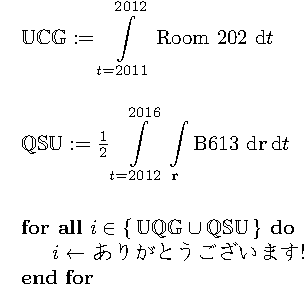
\includegraphics[width=0.4\textwidth]{Preamble/ack_stand/ack_stand}
%\vspace{1ex}
%\end{figure}
%\begin{lstlisting}[breaklines]
$/*$
Firstly, I would like to express my sincerest gratitude to my family back in the 'mel who have always been there for me, and provided amazing support from across the planet since I started my PhD (and before I started too) --- most notably, to Mum, Nan and Maria, who have done so much over the years. Next, my sincerest gratitude and thanks goes to Prof. Thomas Busch, for freeing me from the shackles of a boring job and introducing me to the (ultra)cool world of atomic physics, as well as the guidance he has offered over the years. To past and present members of both the Ultracold Quantum Gases group at University College Cork, and Quantum Systems Unit at OIST, thanks for keeping me sane and helping out through the work and writing over the years --- in no particular order: Mossy, Steve, Jeremie, Tara, Albert, Angela, Sawako, Rashi, James, Irina, the magnificent Dave Rea, and of course Tadhg. Next, I would like to thank the Graduate School for all of their help removing bureaucratic dealings from my everyday life here. A special thanks also goes to the Scientific Computing Section, for allowing me access to some very amazing toys over these past few years. A special thanks also to Annie, for supplying me with enough caffeine to get to the moon and back. Lastly, but not least-ly, to Christina for her compassion, understanding, and assistance over the past few years. $*/$
%\end{lstlisting}


\begin{algorithmic}
\ForAll{$i \in \{S | S \in \textrm{People to thank} \}$}
    \State $i\gets$ ありがとうございます!
\EndFor
\end{algorithmic}

\unnumberedchapter{Abbreviations} 
\chapter*{Abbreviations} 

All abbreviations used in the thesis should be listed here, with their definitions, in alphabetical order.  This includes trivial and commonly used abbreviations (at your own discretion), but not words that have entered into general English usage (such as laser or DNA).  In particular, non-standard abbreviations should be presented here.  This is an aid to the reader who may not read all sections of the thesis. \\ % You can delete this paragraph, only the table is needed.

\begin{longtable}{rl}
PPT & positive partial transpose\\
SRPT & Schr\"odinger-Robertson partial transpose
\end{longtable}
\unnumberedchapter{Glossary} 
\chapter*{Glossary} 

% Break up this table into several ones if it takes up more than one page
\begin{center}
\begin{longtable}{r p{0.58 \textwidth}}
Chemical potential & Energy to overcome for adding an atom to the system
\end{longtable}
\end{center}

\unnumberedchapter{Nomenclature} 
\chapter*{Nomenclature} 

% Break up this table into several ones if it takes up more than one page
\begin{longtable}{rl}
$h$ & Planck constant ($6.626\ 070\ 04\e{-34}\ \mbox{Js}$). \\
$\hbar$ & Planck constant over $2\pi$ ($1.054\ 572\ 66\e{-34}\ \mbox{Js}$). \\
$L_z$ & Angular momentum operator along the $z$-dimension; $xp_y-yp_x$. \\
$\nabla$ & Gradient operator. \\
$\Omega$ & Angular rotation frequency of condensate. \\
$\xi$ & Condensate healing length; the distance from a region of zero density at vortex core to bulk density. \\
$\mu$ & Chemical potential of the condensate; the energy change per unit change in particle number. \\
\end{longtable}
\cleardoublepage
\thispagestyle{empty} % Page style needs to be empty for this page

\vspace*{8cm} 

\hfill
\begin{parbox}{0.6\textwidth}{
\begin{flushright}

If desired, an optional and short dedication may be included here.

\end{flushright}}
\end{parbox}




%----------------------------------------------------------------------------------------
%	LIST OF CONTENTS/FIGURES/TABLES
%----------------------------------------------------------------------------------------

\unnumberedchapter{Contents}
\tableofcontents % Write out the Table of Contents
\unnumberedchapter{List of Figures}
\listoffigures % Write out the List of Figures
\unnumberedchapter{List of Tables}
\listoftables % Write out the List of Tables

%----------------------------------------------------------------------------------------
%	THESIS MAIN TEXT - CHAPTERS
%----------------------------------------------------------------------------------------

\addtocontents{toc}{\vspace{2em}} % Add a gap in the Contents, for aesthetics
\mainmatter % Begin numeric (1,2,3...) page numbering
\newif\ifintro
\introtrue
\ifintro
    \chapter{Introduction} % Title of the unnumbered chapter
        
The purpose of this work was to understand the dynamics of rapidly rotating Bose--Einstein condensates subjected to perturbations, and to develop techniques to control and engineer specific non-equilibrium states. While it is possible to derive some analytical solutions for rapidly rotating condensates (e.g. lowest Landau level approach), such solutions are rare. This thesis concentrates on the numerical solutions of the Gross--Pitaevskii equation, and the resulting dynamics within this framework. It focuses on gaining an understanding of the dynamical behaviour of quantum vortices in an Abrikosov geometry following a perturbation. %A further application of this work would be the use of such tools to model and investigate turbulent and chaotic quantum behaviour.
This body of work was carried out during my time as a Ph.D student at Okinawa Institute of Science and Technology Graduate University (OIST), and grew out of work and ideas I started to pursue at University College Cork (UCC), Ireland.

Understanding ultracold Abrikosov vortex systems can help with engineering quantum states for future technologies. Ideally, these systems can be used for long-term memory storage in quantum computing applications as individual vortices are topologically protected and, therefore, very robust. They also allow the study of quantum mechanical effects on mesoscopic scales, and the inherent periodicity makes them a promising tool for simulating condensed matter physics. Furthermore, perturbed vortex lattices can be used to investigate turbulent, and possibly chaotic, quantum behaviour. While turbulent classical systems are notoriously hard to understand and control, quantum turbulence is thought to offer a more controllable route to understanding the nature of turbulence, due to the quantisation condition of the circulation. It is therefore of large interest to develop new tools for manipulating and engineering specific states of rotating condensates. In the following work I concentrate on two types of perturbations to the equilibrium state of a rotating condensate: i) the modification of the phonon spectrum of the condensate which does not influence the angular momentum, in particular through the use of a kicked optical potential; ii) the direct control of the topological excitations, and hence the angular momentum, which is performed with direct phase engineering of the condensate wavefunction. I examine both in the above order, and investigate their usefulness in controlling and manipulating condensate dynamics.

For investigating these perturbances I assume a system of a rapidly rotating BEC having a large number of vortices, arranged in a triangular Abrikosov lattice pattern. This requires the solution of a two-dimensional partial differential equation at high grid resolution with a variety of different initial conditions and controllable perturbations. The solution of the proposed system is a non-trivial numerical problem, and requires the use of advanced numerical computing techniques to allow for results in a reasonable time. For this I make use of graphics processing unit (GPU) computing, and I will discuss the development of such tools, my numerical contributions, and compare them against conventional simulation techniques.

The thesis is organised as follows:

\section*{Background}
I will first give a brief introduction to the field of cold-atomic gases, and discuss the theoretical framework to describe Bose--Einstein condensation. Emphasis will be placed on material and works relevant to the studies I have performed in this thesis. I will present a derivation of the Gross--Pitaevskii equation, used to model Bose--Einstein condensates, as well as a discussion of the Bogoliubov-de Gennes equations. I will then discuss the hydrodynamic description of the condensate, and give the hydrodynamic form of the Gross--Pitaevskii equation. Here I introduce superfluidity, and the nature of quantised vortices in these systems. I will conclude with an outlook on the cutting edge work in the field in the context of condensate trapping and control.


\section*{Numerical methods}
In this chapter I will discuss methods for numerically solving the Gross--Pitaevskii equation for simulating the dynamics of Bose--Einstein condensates. The Fourier split-operator method will be introduced, as well as the need for imaginary time evolution, and considerations required to effectively simulate the condensate. Graphics processing unit (GPU) computing will be introduced here, with the implementation of the Gross--Pitaevskii equation discussed. To demonstrate the power of GPU computing we will present and solve a difficult numerical problem, namely the solution of an experimentally realistic situation for a single, ultracold atom on an atomchip, for which the treatment of the fully three-dimensional Schr\"odinger equation is required. The use of GPU computing makes this problem tractable in realistic times. The work focuses on the area of adiabatic control techniques, and demonstrates the use of GPU computing to describe the long-time dynamics of a system for observing matter-wave spatial adiabatic passage. This work has been published in  Phys.~Rev.~A~\textbf{88},~053618 (2013) \cite{AO:Morgan_pra_2013}.

\section*{Bose--Einstein condensate dynamics}
In this chapter I will examine the dynamics of Bose--Einstein condensates under rotation, and discuss the methods used for perturbing the condensate system. I begin by introducing the dynamical behaviour of the condensate in the presence of vortices, and introduce a model system used for further discussions. I present the velocity profiles and discuss some of the dynamics a condensate with many vortices is expected to follow. This will be followed by an introduction to the two main perturbation methods for the condensate that I will later use: optical kicking, and phase imprinting. I will also discuss the techniques that I use to analyse the vortex dynamics, concentrating primarily on the kinetic energy spectrum, Delaunay triangulation and Voronoi tessellation.

\section*{Moir\'e superlattice structures}
Here I investigate effects stemming from the optical kicking of a condensate carrying a vortex lattice. The dynamics of the condensate after a kick with an optical potential of the same geometry as the vortex lattice is demonstrated, and shows little to no deviation of ideal vortex positions. However, the resulting condensate density shows the appearance of a superlattice pattern. I analyse this system, and demonstrate that the resulting superlattice pattern stems from interference between the optical kicking potential and the present vortex lattice in reciprocal space. Moir\'e interference theory accurately predicts the observed behaviour, and is backed up by examining the kinetic energy spectrum of the condensate. To conclude, I discuss applications of this optical kicking technique and the resulting moir\'e interference. The results presented in this chapter have been published in Phys.~Rev.~A~\textbf{93}, 023609 (2016) \cite{VTX:oriordan_pra_2016}.

\section*{Defect engineering of the vortex lattice}
To investigate the robustness of a vortex lattice in a rapidly rotating BEC, I will in this chapter discuss the effect of perturbations induced by adding or removing angular momentum through phase imprinting. This technique creates lattice imperfections, with stable topological lattice defects appearing during time evolution. The behaviour of these resulting defects is investigated over long times. I show that the vortex lattice demonstrates highly robust behaviour, even in the presence of such defects. I discuss the use of this method for creating varying degrees of disorder in the lattice, and propose it as a system for investigating transitions from ordered to disordered lattice geometries. The results in this chapter have been accepted for publication in Physical Review A \cite{ME:arxiv_defect}.

\section*{Conclusions and outlook}
In this chapter I conclude the work discussed in the thesis, and discuss extensions, and future ideas for the field.
 % Introduction (unnumbered)

\fi

%%%%%%%%%%%%%%%%%%%%%%%%%%%%%%%%%%%%%%
\newif\iflitrev
\litrevtrue
\iflitrev
    \chapter{Literature review}
        %In this document I review the area of cold atomic gases, and in particular the superfluid behaviour of Bose--Einstein condensate systems. The history of this area will be discussed, highlighting both theoretical and experimental observations. With the fundamentals of Bose--Einstein condensation explained, I will then examine the dynamical behaviour of condensates from the perspective of superfluidity. Vortex behaviour will be discussed, along with recent results, concentrating on the dynamics of vortices in response to external potentials.

 Following this, quantum chaos will be introduced, along with the many of the interesting dynamics that can be observed in superfluid flow. The creation and observation of quantum chaotic dynamics in a Bose--Einstein condensate shall be proposed. The goal of the proposed project will be to generate chaotic dynamics using a vortex lattice subjected to a periodically pulsed optical lattice. Beginning with a well defined state, generation of chaotic behaviour shall be examined. The Hamiltonian required to generate a vortex lattice in a condensate shall be mapped to the delta-kicked harmonic oscillator Hamiltonian, which will provide a model system to understand the observed system dynamics. To characterise the resulting dynamics, the trajectories of the vortices shall be plotted over the course of the evolution of the system. Further information may be obtained by examining the system using phase--space methods and Floquet theory to characterise the observed behaviours. Experiments to observe chaotic behaviour in the quantum regime are rare, and the realisation of this type of system should allow for the first of its kind to observe chaos in a system of well-ordered topological excitations. Given recent experimental progress in the area of trapping, cooling, rotating and controlling Bose--Einstein condensates, the proposed system should be realisable with currently available experimental techniques.
 % Import your chapters here
        \section{Ultracold atoms}\label{sec:coldatoms}
\subsection{Cooling of atomic gases}\label{sub:cooling}
One of the major advances in experimental physics towards creating matter in extreme situations has been the laser cooling of trapped atoms to temperatures near absolute zero. This feat resulted from the pioneering work of C. Cohen-Tannoudji, S. Chu and W.
Phillips, and earned them the Nobel Prize in Physics in 1997 \cite{AO:Chu_revmod_1998,AO:Cohen_revmod_1998,AO:Phillips_revmod_1998}.
It relies on the use of counter-propagating detuned laser fields which are shown at a trapped cloud of atoms. Due to Doppler shifting of the frequencies, atoms moving towards the respective beams see resonant photons, absorb them and slow down due to the momentum absorbed, with this technique being termed ``Doppler cooling''. This is followed by a spontaneous emission in a random direction, for which the recoil kicks average out to zero; hence, the atoms become cooler. As a result, the atoms eventually reach a velocity below that which can be absorbed from the lasers due to the change in resonance frequencies, leaving a narrower velocity distribution. Although laser cooling allowed temperatures to reach micro-Kelvin regimes, additional techniques must be used to obtain atoms deep in the nano-Kelvin temperature range. A further discussion of these methods is presented in [Atomic physics, Foot; Laser cooling and trapping, Metcalf].
I will assume the effectiveness of these techniques to allow the creation of Bose--Einstein condensates in dilute atomic gases.

\subsection{Introduction to Bose--Einstein condensation}\label{sub:becintro}
Bose--Einstein condensation was predicted by N. Bose and A. Einstein \cite{BEC:Ketterle_revmod_2002}. This began as a work on the statistical behaviour of photons, eventually leading to the derivation of the ``Bose--Einstein distribution'' for an ideal bosonic gas.
In the framework of the grand canonical ensemble and following the description given by Pitaevskii and Stringari \cite[chap. 2]{BK:Pitaevskii_Stringari_2003}, the Bose--Einstein distribution is given by
\begin{equation}
\bar{n}_i = \frac{1}{e^{\beta(\epsilon_i - \mu)} -1},
\end{equation}
where $\bar{n}_i$ is the average occupation number of the $i$-th energy state, $\beta=(k_BT)^{-1}$ with $k_B$ being the Boltzmann constant and $T$ as the temperature, $\epsilon_i$ is the $i$-th energy eigenvalue, and $\mu$ is the chemical potential giving the energy required to add an atom to the system.
The total number of particles in the system, $N$, can be evaluated by summing over the individual occupation numbers, as
\begin{equation}
N=\displaystyle\sum_i \bar{n}_i.
\end{equation}
This work predicted that non-interacting, indistinguishable (bosonic) particles would, if their energy was sufficiently low, undergo a phase transition below a critical temperature into a new phase in which the particles would occupy the same lowest lying energy state of the system. The number of atoms occupying this lowest lying state, $N_0$, is given by
\begin{equation}
N_0 \equiv \bar{n}_0 = \frac{1}{e^{\beta(\epsilon_0 - \mu)} - 1},
\end{equation}
with $\epsilon_0$ representing the lowest energy eigenvalue. Since negative occupation numbers would be a nonphysical result, the chemical potential is limited to values of $\mu < \epsilon_0$. As $\mu$ tends to $\epsilon_0$ the occupation of the lowest energy state grows large. Separating the total number of atoms into the lowest lying (condensed), $N_0$, and higher lying (thermal), $N_T$, states as
\begin{equation}
N = N_0 + N_T = N_0 + \displaystyle\sum_{i\neq 0}\bar{n}_i(T,\mu),
\end{equation}
a relation for the the onset of Bose--Einstein condensation can be given. For a finite temperature system ($T>0$) this will happen when the temperature drops below a critical value, $T_c$, where $\mu$ will approach $\epsilon_0$, resulting in the macroscopic occupation of the lowest lying state, yielding a Bose--Einstein condensate (BEC).

BECs of ultracold atomic gases are a prime example of coherent matter waves, and demonstrate quantum mechanical effects on length-scales which can be considered mesoscopic. Given a cloud of identical bosons at higher temperature, the atoms exhibit billiard-ball type behaviour. As they are cooled, their thermal de Broglie wavelength increases as
\begin{equation}
\lambda_{dB} = \sqrt{\frac{\hbar^2}{2\pi mk_{B}T}},
\end{equation}
where $m$ is the atom mass, because the wave-nature of the atoms becomes more prominent, and the de Broglie waves start to overlap when $\lambda_{dB} \approx$ inter-particle separation. The quantity $n\lambda_{dB}^3$, where $n$ is the density of the gas, is known as the \emph{phase-space density}. Physically this denotes the number of particles present in a box with sides of $\lambda_{dB}$ length, and the phase transition to the condensate sets in at $\zeta\left(\frac{3}{2}\right)$, where $\zeta$ is the Riemann-Zeta function \cite{BK:Ueda_2010}. The value of $T_c$ for this to occur in a uniform gas is given by
\begin{equation}
k_BT_c = \frac{2\pi}{\zeta\left(\frac{3}{2}\right)^{2/3}}\frac{\hbar^2n^{2/3}}{m}.
\end{equation}
For a finite number of atoms in a realistic experimental scenario one can consider the case of a BEC trapped in a harmonic oscillator potential. For this finite-sized sample, and inhomogeneous density profile, the transition temperature is given by
\begin{equation}
k_BT_c = \frac{\hbar\bar{\omega}N^{1/3}}{\zeta(3)^{1/3}},
\end{equation}
where $\bar{\omega}=(\omega_x\omega_y\omega_z)^{1/3}$ is the geometric mean of the oscillator frequencies. Critical temperatures for harmonically trapped gases are on the order of nano-Kelvin assuming realisable trapping frequencies, which were experimentally inaccessible during the time of Bose and Einstein.

Fritz London, in 1938, following on from the body of work derived by Einstein and Bose drew the connection between superfluidity in liquid $^4$He and Bose--Einstein condensation \cite[Chap.~1]{BK:Pitaevskii_Stringari_2003}. However, due to the liquid nature of $^4$He at low temperatures only approximately $10\%$ of the atoms condense into a BEC \cite{BEC:Penrose_pr_1956}. In order to achieve the large occupation of the lowest energy state the system must be prepared so that the interparticle interaction strength does not destroy the coherence, as is the case for liquid $^4$He.

Due to their weak interactions, dilute atomic gases are closer to the ideal case discussed by Bose and Einstein. One negative impact, though, were the higher masses of the atoms used in such systems, which required reaching much lower transition temperatures. As such, the use of lighter elements were considered. Spin-polarised hydrogen
was one of the first systems to be investigated to create BEC \cite{BEC:Kleppner_enfe_1998,BK:Pitaevskii_Stringari_2003} in the 1970's. Using trapping and cooling techniques
present at the time, this type of system came close, but did not quite reach the required temperatures and phase-space densities for
Bose--Einstein condensation to occur until over twenty years later \cite{BEC:Fried_prl_1998}. Given the advent of laser cooling in the 1980's, the use of alkali atoms was considered partly due to the ease of accessibility of their optical transition frequencies. It was not until 1995 that the first BECs would be experimentally realised \cite{BEC:Cornell_science_1995,BEC:Ketterle_prl_1995}.

\subsection{Theoretical description of BECs: Gross--Pitaevskii equation}\label{sub:gpederiv}
I will, in the following section, outline the derivation of the mean-field Gross--Pitaevskii equation, which is widely used to study the behaviour of the condensate in many works cited in this review. Following the \textit{Les Houches 2013 Lecture Course} by J. Walraven \cite{LEC:Walraven_lh_2013} the second quantization form of the many-body Hamiltonian for interacting particles in an external potential is given by
\begin{equation}\label{eqn:ham2ndq}
\hat{\mathcal{H}} = \hat{H_1} + \hat{H_2} = \int \hat{\Psi}^{\dagger} H_0\left(\textbf{r},\textbf{p} \right)  \hat{\Psi} \; d\textbf{r}  + \frac{1}{2} \int\hat{\Psi}^{\dagger}\hat{\Psi}^{\dagger}V_{\textrm{int}}(\textbf{r}^\prime-\textbf{r})\hat{\Psi}\hat{\Psi} \; d\textbf{r}^\prime d\textbf{r},
\end{equation}
with $H_0\left(\textbf{r}, \textbf{p} \right) = -\frac{\hbar}{2m}\nabla^2 + V_{\textrm{ext}}\left(\textbf{r}\right)$. The external potential, $V_{\text{ext}}(r)$ is taken as harmonic, of the form
\begin{equation}
V_{\text{ext}}(\textbf{r}) = \frac{m}{2}\displaystyle\sum_{i}{\omega_i r_i},
\end{equation}
and with $\omega_i$ representing the trapping frequency in the $i$-th spatial dimension. The interaction potential, $V_{\text{int}}$ is assumed to be point-like as
\begin{equation}\label{eqn:v_int}
	V_{\text{int}}\left(\textbf{r}_i,\textbf{r}_j \right) = g\delta\left(\textbf{r}_i - \textbf{r}_j\right),
\end{equation} where $\delta$ is the Dirac delta function and the mean-field interaction, $g$ is given by
\begin{equation}
	g = \frac{4\pi\hbar^2 a_s}{m},
\end{equation}
with $a_s$ being the s-wave scattering length. Inserting the contact potential Eq. \eqref{eqn:v_int} into the second quantised interaction Hamiltonian $\hat{H}_2$ from Eq. \eqref{eqn:ham2ndq} above yields the following relations
\begin{subequations}
\begin{align}
\hat{H}_2 &= \frac{g}{2} \int \hat{\Psi}^{\dagger}(\textbf{r})\hat{\Psi}^{\dagger}(\textbf{r\textprime}) \delta\left(\textbf{r} - \textbf{r\textprime}\right)\hat{\Psi}(\textbf{r\textprime})\hat{\Psi}(\textbf{r})d\textbf{r}d\textbf{r\textprime} \\
 & = \frac{g}{2}\int \hat{\Psi}^{\dagger}(\textbf{r})\hat{\Psi}^{\dagger}(\textbf{r}) \hat{\Psi}(\textbf{r})\hat{\Psi}(\textbf{r})d\textbf{r}d\textbf{r} \\
 & = \frac{g}{2}\int \hat{\Psi}^{\dagger}\left(\textbf{r}\right)\hat{n}\left(\textbf{\textbf{r}}\right)\hat{\Psi}^{\dagger}d\textbf{r}.
\end{align}
\end{subequations}

In the Heisenberg picture, the evolution of the system is governed by the equation
\begin{equation}\label{eqn:heisenberg}
i\hbar \frac{\partial}{\partial t}\hat{\Psi}_H\left(\textbf{r}, t\right) = \left[\hat{\Psi}_{H}\left(\textbf{r}, t\right), \hat{\mathcal{H}}  \right],
\end{equation}
where the Heisenberg field annihilation operator, $\hat{\Psi}_H\left(\textbf{r}, t\right)$, is given by
\begin{equation}\label{eqn:psi_heisenberg}
\hat{\Psi}_H\left(\textbf{r}, {t} \right) = e^{\frac{i\hat{\mathcal{H}}t}{\hbar}}\hat{\Psi}\left(\textbf{r}\right) e^{\frac{-i\hat{\mathcal{H}}t}{\hbar}}.
\end{equation}
The operator, $\hat{\Psi}_H$ can be interpreted as the one removing an atom from a given state of the system. Therefore, if all $N$ atoms in the system are in the ground-state, $\vert 0_N\rangle$, as would be the case in an ideal condensate, the following relationship holds
\begin{subequations}
\begin{align}
\hat{\Psi}_{H}(\textbf{r},t)\vert 0_N \rangle &= e^{\frac{iE_0(N-1)t}{\hbar}}\hat{\Psi}(\textbf{r})e^{\frac{-iE_0(N)t}{\hbar}}\vert 0_N \rangle \\
&= \hat{\Psi}(\textbf{r})e^{\frac{i[E_0(N-1) - E_0(N)]t}{\hbar}} \vert 0_N \rangle \\
&= \hat{\Psi}(\textbf{r})e^{\frac{-i\mu t}{\hbar}} \vert 0_N \rangle,\label{eqn:psi_dagger_time} \label{eqn:stationary_soln}
\end{align}
\end{subequations}

where $\mu=E_0(N) - E_0(N-1)$ is the chemical potential. Using the bosonic commutation relations
\begin{eqnarray}
\left[\hat{\Psi}(\textbf{r}'), \hat{\Psi}^{\dagger}(\textbf{r})\right] &=& \delta(\textbf{r}' - \textbf{r}), \\
\left[\hat{\Psi}(\textbf{r}'), \hat{\Psi}(\textbf{r})\right] &=& \left[\hat{\Psi}^{\dagger}(\textbf{r}'), \hat{\Psi}^{\dagger}(\textbf{r})\right] = 0,
\end{eqnarray}
and noting the following relations
\begin{align}
\left[\hat{\Psi}(\textbf{r}),\hat{H}_1 \right] & = \hat{H}_0(\textbf{r},\textbf{p})\hat{\Psi}(\textbf{r}), \\
\left[\hat{\Psi}(\textbf{r}),\hat{H}_2 \right] & = g\hat{n}(\textbf{r})\hat{\Psi}(\textbf{r}), \\
\left[\hat{\Psi}(\textbf{r}),\hat{N} \right] & = \hat{\Psi}(\textbf{r}) ,
\end{align}
upon substitution of Eq.~\ref{eqn:psi_dagger_time} into Eq.~\ref{eqn:heisenberg}, it be rewritten as
\begin{equation}\label{eqn:almost_gpe}
    i \hbar \partial_t \left( \hat{\Psi}(\textbf{r}) e^{-\frac{i\mu t}{\hbar}} \right) = H \hat{\Psi}(\textbf{r}) e^{-\frac{i\mu t}{\hbar}}
\end{equation}
with
%\begin{equation}\label{eqn:h_many}
%\mathcal{H} = \displaystyle\sum\limits_{i=1}^N \left( -\frac{\hbar^2}{2m}\nabla^2  + V(\textbf{r}_i)\right) + \frac{1}{2}g\displaystyle\sum\limits_{i\neq j}\delta(\textbf{r}_i - \textbf{r}_j).
%\end{equation}
\begin{equation}\label{eqn:h_many}
H =  -\frac{\hbar^2}{2m}\nabla^2  + V(\textbf{r}) + g\hat{n}(\textbf{r}).
\end{equation}
Due to the macroscopic occupation of the lowest lying single-particle state, $\hat{\Psi}$ can be treated as the sum of a condensed term and a quantum fluctuation (uncondensed) term, as
\begin{equation}\label{eqn:gpe_fluc}
    \hat{\Psi} = \Psi + \delta\hat{\Psi}.
\end{equation}
Substituting Eq.~\ref{eqn:gpe_fluc} into \ref{eqn:ham2ndq}, taking terms in $\Psi$, and following the above procedure gives the time dependent mean-field Gross--Pitaevskii equation (GPE) as
\begin{equation}\label{eqn:gpe}
i\hbar\frac{\partial}{\partial t}\Psi(\textbf{r},t) = \left[-\frac{\hbar^2}{2m}\nabla^2 + V(\textbf{r}) + g\vert\Psi(\textbf{r},t)\vert^2 \right]\Psi(\textbf{r},t),
\end{equation}
where $\Psi(\textbf{r},t) = \Psi(\textbf{r})e^{-\frac{i\mu t}{\hbar}}$.
Assuming a zero-temperature condensate, the number of uncondensed atoms will be zero, and thus one can we can safely ignore all terms in $\delta\hat{\Psi}$, all of which are order greater than unity. The remaining condensed term is of the form of a classical field, wherein the problem moves from a quantum one to semiclassical. The time independent form can be found by evaluating the left-hand side derivative and dividing across by $e^{-\frac{i\mu t}{\hbar}}$, yielding
\begin{equation}
\mu\Psi(\textbf{r}) = \left[-\frac{\hbar^2}{2m}\nabla^2 + V(\textbf{r}) + g\vert\Psi(\textbf{r},t)\vert^2 \right]\Psi(\textbf{r}),
\end{equation}
where the wavefunction is normalised to the particle number, $N$, as follows
\begin{equation}\label{eqn:norm}
\displaystyle\int\limits_{-\infty}^{\infty}d\textbf{r} \left\vert \Psi\left(\textbf{r}\right) \right\vert^2 = N.
\end{equation}
In the case of a rotating condensate an additional term appears in the GPE, $-\Omega L$, where $\Omega$ is the angular rotation frequency, and $L$ is the angular momentum. Assuming rotation about a single axis, the longitudinal direction, $z$, $L$ can be replaced with $L_z$, giving the final form of the GPE in the co-rotating frame as
\begin{equation}\label{eqn:gpe_rotation}
i\hbar\frac{\partial}{\partial t}\Psi(\textbf{r},t) = \left[-\frac{\hbar^2}{2m}\nabla^2 + V(\textbf{r}) + g\vert\Psi(\textbf{r},t)\vert^2 - \Omega L_z  \right]\Psi(\textbf{r},t).
\end{equation}
This mean-field equation can be used to describe the behaviour of the condensate, provided the number of atoms is sufficiently large ($>10^3$ for most experimental set-ups) and the correlations are not too strong. Assuming a large number of bosons in the condensate, $N$, the interaction term dominates over the kinetic term of the Hamiltonian which can therefore be neglected. This turns finding the ground-state of the system into a solvable, algebraic problem, and is known as the Thomas-Fermi approximation \cite[~p. 84]{BK:Ueda_2010}. The Hamiltonian can thus be reduced to a combination of the trapping potential and the mean-field interaction, and the wavefunction, $\psi_{\textrm{TF}}$, can be determined from the time independent GPE as
\begin{equation}
\psi_{TF}(\textbf{r}) = \sqrt{ g^{-1}[\mu - V(\textbf{r})] \Theta(\mu - V(\textbf{r}))},
\end{equation}
where $\mu$ is the chemical potential, and $\Theta$ is the Heaviside step function, which ensures that the condensate density does not become negative. Within this regime the condensate can be described by hydrodynamical equations \cite[Pg.~180]{BK:Pitaevskii_Stringari_2003}, and from this, an approximate value for the cloud radius can be determined, called the Thomas-Fermi radius. The boundary of the cloud is determined by the surface at which the density becomes zero, and corresponds to the point where the trapping potential and chemical potential are equivalent. This gives the geometric mean spatial extent of the cloud \cite[~p. 169]{BK:Pethick_Smith_2008} as
\begin{equation}
\bar{R} = \left(\frac{15Na}{\bar{a}}\right)^{1/5}\bar{a},
\end{equation}
where the characteristic length of the harmonic oscillator is given by
$\bar{a} = \sqrt{{\hbar}/{m\bar{\omega}}}$. Thus, within the Thomas-Fermi radius, it is possible to explain the behaviour of the BEC analytically and compare with exact numerical results from integrating the full GPE.

\subsection{Bogoliubov-de Gennes equations}
\label{sec:bogo}
While the Gross--Pitaevskii equation captures the rich array of dynamics exhibited by a condensate system, it is often necessary to examine the stability of its solutions. Where earlier I neglected the small quantum fluctuations (see eq. \ref{eqn:gpe_fluc}), we can instead reformulate this term as a combination of counterpropagating waves with the stationary state solution as
\begin{equation}
    \delta\hat{\Psi} = \exp\left(\frac{-i\mu t}{\hbar}\right)[u\exp(-it\omega) + v^{*}\exp(it\omega)].
\end{equation}
Taking this expression where $\mu$ is the chemical potential of the condensate, the wavefunction can be defined as
\begin{equation}\label{eqn:bogo_psi}
\Psi(\mathbf{r},t) = \exp\left(-i\frac{\mu t}{\hbar}\right)[\Psi_0(\mathbf{r}) + u(\mathbf{r})\exp\left(-i\omega t\right) + v^{*}(\mathbf{r})\exp\left(i\omega t\right) ],
\end{equation}
where $\Psi_0(\mathbf{r})$ is the stationary state solution.

Firstly, we calculate the time-derivative of eq. \ref{eqn:bogo_psi}, which after simplification becomes
\begin{equation}\label{eqn:bogo_lhs}
    i\hbar\partial_t \Psi(\mathbf{r},t) = \exp\left(\frac{-i\mu t}{\hbar}\right)\left[\mu\Psi_0 + (\mu+\hbar\omega)u\exp\left(-it\omega\right) + (\mu+\hbar\omega)v^{*}\exp\left(it\omega\right) \right],
\end{equation}
where I have dropped the dependence on $\mathbf{r}$ for notational simplicity. Next, the nonlinear interaction term is given as
\begin{subequations}
\begin{align}\label{eqn:bogo_nonlin}
    g|\Psi|^2\Psi &= g \Psi_0^{*}\Psi_0\Psi_0 \\
                &= g\exp\left(\frac{-i\mu t}{\hbar}\right)\left(\Psi_0^{*} + u^{*}\exp(i\omega t) + v\exp(-i\omega t)\right)\left(\Psi_0 + u\exp(-i\omega t) + v^{*}\exp(i\omega t)\right)^2, \\
                & \approx g\exp\left(\frac{-i\mu t}{\hbar}\right)\left[
                |\Psi_0|^2\left(
                 \Psi_0 + 2(u\exp\left(-i\omega t\right) + v^{*}\exp\left(i\omega t\right) )\right) + \Psi_0^2\left( u^{*}\exp\left(i\omega t\right) + v\exp\left(-i\omega t\right)
                \right)
                \right].
\end{align}
\end{subequations}

Plugging these terms into the GPE, and linearising in terms of $u$ and $v$ yields the Bogoliubov-de Gennes equations,
\begin{subequations}\label{eqn:bogo_lhsrhs}
\begin{align}
    \mu \Psi_0 &= (H_0 - \Omega L + g |\Psi_0|^2)\Psi_0,\\
    (\mu +\hbar\omega)u &= (H_0 - \Omega L + 2g|\Psi_0|^2)u + g\Psi_0^2 v,\\
    (\mu +\hbar\omega)v^{*} &= (H_0 - \Omega L + 2g|\Psi_0|^2)v^{*} + g\Psi_0^2 u^{*},
\end{align}
\end{subequations}
where
\begin{equation}\label{eqn:bogo_h0}
H_0 = -\frac{\hbar^2}{2m}\nabla^2 + V(\mathbf{r})
\end{equation}
This can be written as a matrix as
\begin{equation}
    \begin{pmatrix}
        H_0 - \mu -\Omega L_z & g\Psi_0^2 \\
        -g\Psi_0^{*2} & -H_0 + \mu +\Omega L_z
    \end{pmatrix}
    \begin{pmatrix}
        u \\
        v
    \end{pmatrix}
    = \hbar\omega
    \begin{pmatrix}
        u \\
        v
    \end{pmatrix}
\end{equation}
where the eigenvalues of these modes can be used to determine the stability of the system. The norm of these values is given by $\int d\mathbf{r}(|u|^2 - |v|^2)$. If the norm is positive, with positive eigenvalues, we can say the system is stable. If the norm is negative, the system will have an energetic instability. This will cause the system to move towards the lowest energy state only in the presence of dissipation. If, however, the norm is 0 with imaginary eigenvalues, the modes of fluctuations are dynamically unstable. Due to the complex eigenvalues over time the mode will dominate exponentially and destroy the initial state of the condensate. %In a later section I  will use this approach later to examine the behaviour of the Bose--Einstein condensate.

\subsection{Lower dimensional condensates}\label{sub:coldatom_recent}
Whilst the full 3D dimensional GPE describes the dynamics of a condensed cloud of cold atoms, often the physics of lower dimensional systems can be quite fruitful. For a BEC tightly confined along one axis, the system can be described as a pancake shaped condensate, or cigar shaped for tight confinement along two axes. These teightly confined systems allow for the examination of both two and one dimensional physics. For a BEC harmonically confined in a trap with a transverse frequency, $\omega_\perp$, and tightly confined along $z$ with frequency $\omega_z >> \omega_\perp$, all dynamics can be frozen out along $z$, leaving the system in the groundstate of the oscillator along $z$. This assumes that the energy to excite the system along $z$, $\hbar\omega_z$ is significantly greater than that to excite along the transverse plane $\hbar\omega_\perp$. This assumption allows for the wavefunction to be written as $\Psi(\mathbf{r},t) = \Psi(x,y,t)\phi(z)$ where $\mathbf{r} = [x,y,z]$, $\Psi(x,y,t)$ is the transverse wavefunction, and $\phi(z) = \left(\frac{m\omega_z}{\pi\hbar}\right)e^{-\frac{m\omega_z}{2\hbar}z^2}$ is the groundstate along $z$.
Substituting this separable wavefunction into the GPE and integrating over all space with respect to $z$ modifies the nonlinear interaction strength as
\begin{equation}
    g^{\prime} = g\sqrt{\frac{m\omega_z}{2\pi\hbar}}.
\end{equation}
Though still technically a 3D system, by integrating along the stationary axis the net effect gives an effective interaction strength for a \textit{quasi}-2D model. Provided the previous assumptions hold for the trapping frequencies, the system can be modeled in two-dimensions without any loss of generality. A major advantage of the confinement of a BEC to a two-dimensional pancake geometry is the added stability of excitations. For all work and models discussed later I will assume a quasi-2D condensate.
 % Import your chapters here
        \section{Superfluidity}\label{sec:superfluid}
\subsection{Introduction to superfluidity}\label{sec:intro_super}

Superfluidity is a macroscopic quantum effect that is closely related to Bose--Einstein condensation. Liquid helium has been known for many years to exhibit superfluid behaviour \cite{BEC:Penrose_pr_1956}. One interesting property of superfluids is that they have quantized circulation which can lead to the appearance of quantum vortices under rotation. Traditionally, such excitations have been created in liquid $^4$He by a ``rotating bucket'' type of experiment, where the container holding the superfluid is rotated about a single axis. When the fluid is initially above the $\lambda$-critical point, the temperature at which $^4$He moves from a classical fluid to a superfluid, the atoms will undergo rotation with the container due to viscous effects. On cooling the atoms below the $\lambda$-critical point, liquid $^4$He will undergo a transition to the superfluid state. If the velocity is above a critical rotation frequency, $\Omega_c$, vortices are nucleated in the rotating superfluid helium system. Due to the strongly interacting nature of liquid helium, the nucleated vortices are difficult to visualise as the healing length, $\xi$, of liquid $^4$He is only on the order of {\r{A}}ngstr{\"o}ms \cite{BEC:Srinivasen_pramana_2006}.

In order to visualise these vortices experimentally it was necessary to use an indirect means of visualisation in the form of tracer particles \cite{BEC:Packard_physb_1982}. Limited success was had with this technique using solid hydrogen, and later plastic microspheres, as they tended to join together due to static charges. An improved technique, using charged particles, showed much greater success \cite{Vtx:Packard_prl_1969}. Ions, or electrons, were trapped inside the vortex lines, and an electric field along the direction of the lines allowed for acceleration of the charges towards a luminescent screen where they could be observed. Current experimental work in vortex visualisation with liquid $^4$He has advanced significantly \cite{Vtx:Tsubota_arxiv_2010,Vtx:Guo_pnas_2014}, yet fine control over the behaviour of the liquid and the vortex dynamics remains difficult.

%\todo[inline]{Derive hydrodynamic formalism for GPE}
Superfluid behaviour is observed in liquid helium due partly to a portion of the atoms condensing into the ground state. Given that BECs show superfluidity, the use of a dilute gas where the majority of atoms are in the condensate state provides a more controlled means to investigate superfluidity and quantised vortices \cite{BK:Ueda_2010,BEC:Srinivasen_pramana_2006,Vtx:Tsubota_arxiv_2010,CT:Tsubota_jpsj_2008}. In contrast with liquid $^4$He, which has a healing length of the order of {\r{A}}ngstr{\"o}ms, the healing length of a dilute gas of alkali atoms is on the order of microns \cite{Vtx:Isoshima_pra_1999}. This places condensates in a much more accessible regime for visualising vortices compared with liquid $^4$He experiments. For many condensates visualisation of the vortices is provided by absorption imaging, following a time-of-flight expansion of the cloud to allow the vortex cores to expand and become more easily visible~\cite{Vtx:Raman_prl_2001,VTX:Rankonjac_pra_2016}. One drawback of this method is that it is destructive, and requires multiple experimental realisations to acquire any dynamical information. To examine the dynamics of the vortices, successive imaging techniques are required. Single-shot experiments have been demonstrated, where a small percentage of the condensate is repeatedly transferred to an untrapped atomic state. This allows for the untrapped atoms to expand, and vortices have been imaged this way~\cite{VTX:Freilich_sci_2010}. With this method the precession of the vortices in a trapped condensate can be directly observed, in a single-shot experiment. More recently, \textit{in-situ} imaging of a condensate with a vortex lattice was demonstrated and allowed resolution of the cores without time-of-flight expansion with a minimally destructive optical refraction technique~\cite{VTX:Wilson_pra_2015}.

To fully understand the behaviour of these systems, it is necessary to have a framework for modeling the condensate, in the absence and the presence of vortices. As described above, a dilute gas of condensed atoms close to absolute zero temperature can be readily modelled by the Gross--Pitaevskii equation \eqref{eqn:gpe_rotation}, offering a direct means to examine condensate behaviour. It is, however, useful to obtain a hydrodynamic description for the condensate, performed by treating its wave-function as
\begin{equation}\label{eqn:madelung}
\Psi(\textbf{r},t) = \sqrt{\rho(\mathbf{r},t)} e^{\textrm{i}\theta(\textbf{r},t)},
\end{equation}
with
\begin{equation}\label{eqn:density}
\rho(\textbf{r},t) = \Psi^*(\textbf{r},t)\Psi(\textbf{r},t) = \vert \Psi (\textbf{r},t) \vert ^2.
\end{equation}
where $\theta(\textbf{r},t)$ is the condensate phase \cite{BK:Pitaevskii_Stringari_2003}. Following the formalism given by Pitaevskii and Stringari \cite{BK:Pitaevskii_Stringari_2003} and multiplying Eq.~\eqref{eqn:gpe} by $\Psi^{*}(\mathbf{r},t)$ then subtracting the complex conjugate of that expression allows one to obtain the continuity equation as
\begin{equation}\label{eqn:continuity}
\frac{\partial}{\partial t}\rho(\textbf{r},t)  + \nabla\cdot \textbf{j}(\textbf{r},t) = 0,
\end{equation}
where the current density of the condensate is
\begin{equation}\label{eqn:current_density}
\textbf{j}(\textbf{r},t) = \frac{-\textrm{i}\hbar}{2m}\left[\Psi^*(\textbf{r},t)\nabla\Psi(\textbf{r},t) - \Psi(\textbf{r},t)\nabla\Psi^*(\textbf{r},t)\right].
\end{equation}
Using ansatz \eqref{eqn:madelung} and substituting it into Eq. \eqref{eqn:current_density} then gives the form for the current density,
\begin{equation}
\textbf{j}(\textbf{r},t) = \vert\Psi(\textbf{r},t)\vert ^2\frac{\hbar}{m}\nabla\theta(\textbf{r},t).
\end{equation}
The velocity of the superfluid, $\textbf{v}(\textbf{r},t)$, is defined as the ratio of the current density to the density, which is then given by
\begin{equation}\label{eqn:velocity}
\textbf{v}(\textbf{r},t)\equiv \frac{\textbf{j}(\textbf{r},t)}{\rho(\textbf{r},t)} = \frac{\hbar}{m}\nabla\theta(\textbf{r},t).
\end{equation}
The gradient of the phase therefore determines the velocity of the condensate atoms; this indicates that the superfluid behaviour in a condensate is irrotational ($\nabla\times(\nabla\theta) =0$). Assuming a closed loop integral about a central point in the condensate, and recalling the single-valued nature of the wavefunction, yields the relationship
\begin{equation}\label{eqn:circulation}
\oint \textbf{v}\cdot d\textbf{l} = \frac{\hbar}{m}2\pi l.
\end{equation}
This shows the quantised nature of circulation in a superfluid, with $l$ representing the integer charge of the circulation. The phase winding around the central region is given by multiples of $2\pi$, with the centre of the phase becoming ill-defined. To circumvent this problem the density at this point drops to zero, signalling the presence of a vortex in the condensate. This drop happens over the scale of the healing length, which, for repulsive interactions, is given by
\begin{equation}
\xi = \frac{1}{\sqrt{8\pi \rho_b a_s}},
\end{equation}
where $\rho_b$ is the bulk density of the condensate, and $a_s$ is the $s$-wave scattering length. For a cylindrically symmetric rotating condensate carrying a single vortex in its centre the wavefunction can be written as
\begin{equation}\label{eqn:madelung_l}
    \Psi = |\Psi|e^{\textrm{i}l\theta},
\end{equation}
where $l$ is the vortex charge. The velocity profile at a distance $r_{v}$ away from the core can then be given as
\begin{equation}\label{eqn:1_over_r}
    v =\frac{\hbar l}{m r_v}.
\end{equation}

To sustain a vortex the condensate must have sufficient angular momentum, which is imparted via the angular rotation frequency times the angular momentum operator $-\Omega L_z$ in the Hamiltonian given by Eq. \eqref{eqn:gpe_rotation}. The rotation frequency, $\Omega$, of the condensate has an upper-bound stability limit equivalent to the transverse trapping frequency, $\omega_{\perp}$, of the harmonically trapped condensate.
%\todo[inline]{Find a better home for speed of sound}

\subsection{Vortices in Bose--Einstein condensates}\label{ss:vorticesinbec}

Given that the circulation of a vortex in a superfluid is quantised, one may assume that for faster rotation rates the circulation increases in integer multiples of $h/m$, beyond critical rotation thresholds to excite each higher multiple. To understand the effect of vortex charge on the condensate, it is necessary to examine the energy functional, as given by
    \begin{equation}\label{eqn:functional}
        E[\Psi] = \int \Psi^{*} (H_{\text{E}}) \Psi d\mathbf{r},
    \end{equation}
where $H_{\text{E}} = (-\hbar^2/2m)\nabla^2 + V + g|\Psi|^2/2 - \Omega L_z$. By substituting \eqref{eqn:madelung_l} into Eq.~\eqref{eqn:functional} the energy functional is given as
\begin{equation}\label{eqn:functional_full}
    E[\Psi] = \int \frac{\hbar^2}{2m} \left(|\nabla\Psi|^2  + \frac{|\Psi|^2 l^2 m \mathbf{v}^2}{2}  \right) + V|\Psi|^2 + \frac{g}{2}|\Psi|^4 + \Omega \Psi^{*} L_z \Psi,
\end{equation}
where $\mathbf{v}$ is the superfluid velocity, as given by Eq.~\eqref{eqn:velocity}. The $l^2$ term shows that the energy scales quadratically with an increase in charge. This energy growth dependence indicates that it will be more favourable to allow for two singly charged vortices, than a single doubly charged vortex, which will decay due to the presence of complex eigenmodes \cite{VTX:Kawaguchi_pra_2004}. For rates of rotation $\Omega_c < \Omega < \omega_\perp$, where $\Omega_c$, is the threshold rotation rate to create a vortex, the condensate will favour many singly quantised vortices, rather than one or several multiply charged ones. For a superfluid condensate in the rotating frame $\Omega_c = {E_v/L} = {E_v/(N\hbar)}$, where $E_v$ is the energy of the vortex, and $L$ is the angular momentum component of the superfluid along $z$~\cite{BK:Pitaevskii_Stringari_2003}.

The stability of vortex states in a condensate is also a widely discussed topic \cite{Vtx:Fedichev_pra_1999,Vtx:Feder_prl_1999}, as non-rotating traps show an instability for small displacements of the vortex from the trap centre. Since the ``rotating bucket'' technique used to generate vortices in $^4$He cannot be used for gaseous BECs, many other techniques have been developed \cite{Vtx:Anglin_prl_1999,Vtx:Davies_prl_1999,Vtx:Marshall_pra_1999,Vtx:Dobrek_pra_1999,VTX:Nakahara_physb_2000}. For the work presented in this thesis, the method proposed by Dobrek \textit{et al}. \cite{Vtx:Dobrek_pra_1999}, is of particular interest, as it allows one to optically generate vortices by the use of what they term a ``phase-imprinting'' method. The authors describe a scheme where the phase of the condensate is directly controlled in such a way that the required topological charge to induce a vortex during evolution is provided by external lasers. Through use of an absorption plate whose absorption coefficient depends on the axis angle, the condensate can be imprinted with the required phase pattern. This method will form the basis of one work carried out in this thesis, and will be discussed in detail later in Sec.~\ref{sec:phase}.


\subsection{Vortex lattices}\label{sec:sec2_vtxlatt}

Although a large number of works exist which investigate systems with low numbers of vortices \cite{THS:Davies_2000,Vtx:Chevy_prl_2000,Vtx:Cooper_prl_2001,Vtx:Rosenbusch_prl_2002,Vtx:Ogawa_pra_2002,Vtx:Bretin_joptb_2003,Vtx:Madison_prl_2000,Vtx:Madison_jmo_2000,Vtx:Chevy_aoi_2001,Vtx:Madison_prl_2001,Vtx:Mottonen_jpcm_2002}, such systems do not necessarily form periodic vortex lattices. We will therefore concentrate primarily on studies of systems containing many vortices, assuming large values of $\Omega \lesssim \omega_\perp$. For such systems, the vortices are arranged in a periodic triangular Abrikosov lattice, reminiscent of that which appears in type-II superconductors with magnetic flux lines \cite{Vtx:AboShaeer_sci_2001}. Experimental setups have demonstrated upwards of over 130 vortices in a well ordered triangular formation. The resulting lattices are shown to be highly stable and are ideal setups for investigations of periodic systems \cite{Vtx:AboShaeer_sci_2001,Vtx:Engels_prl_2002}.

The Thomas--Fermi limit discussed earlier describes the case where the kinetic energy term of the Hamiltonian may be neglected in comparison to the interaction energy, as it offers little contribution to the condensate behaviour. This remains true for low rotation rates, however kinetic energy becomes important in the limit of fast rotation. In this case $\Omega/\omega_{\perp}\approx 1$, and the centrifugal force term, $m\Omega^2r$, almost balances with the trapping force term, $-m\omega^2r$. The condensate behaviour then closely resembles that of the two-dimensional quantum Hall regime, where the system is residing in the lowest Landau level, (LLL) ($n=0$) \cite{Vtx:Ho_prl_2001}.  As the rotation of the cloud approaches the trapping frequency, the system tends to the LLL, wherein the nonlinear interaction term becomes relatively weak due to the centrifugal forces on the atomic cloud. In this regime the Thomas--Fermi approximation becomes invalid, as the interaction term no longer dominates over the kinetic energy. The interaction energy is then much smaller than the gap between energy levels for single particle Landau levels. While there have been studies using harmonic-plus-quartic potentials to allow condensates to remain trapped beyond the harmonic trapping frequency limit \cite{BEC:Bretin_prl_2004,Vtx:Ghosh_pra_2004}, we will in this thesis consider only systems in a harmonic confinement.

At high rotation rates very close to the trap frequency ($\Omega/\omega_\perp \approx 1$) the system enters a fractional quantum Hall (FQH) state~\cite{Vtx:Regnault_prl_2003}, and will require treatment beyond that of mean-field methods. This state will require the use of a discrete boson model, which becomes next to impossible to simulate for a realistic number of atoms in a condensate. However, for rotation rates just below this limit a mean-field approach can be used in the so-called ``mean-field quantum Hall'' (MFQH) regime~\cite{BEC:Fetter_revmodphys_2009}. The differences between these two regimes are characterised purely by the ratio of the kinetic energy to the interaction energy of the system, and in the MFQH regime we can assume that the LLL has been achieved~\cite{Vtx:Zhai_pra_2004,BEC:Stock_laserphyslett_2005}. To identify these different regimes one may use the the ``filling factor'', $\nu=N/N_v$ \cite{BK:Ueda_2010,Vtx:Ho_prl_2001}, which examines the ratio of atoms to vortices in the system. This becomes an important characteristic at high rotation rates, and in the case where $1000 > \nu > 10$, the system may be accurately described to be in the MFQH regime. For values $\nu \leq 10$ the system is said to be strongly correlated~\cite{BEC:Fetter_revmodphys_2009}, and the system enters the FQH regime. For an almost perfectly regular vortex lattice, the rotation rate must be sufficiently large so that the condensate width extends to large distances and a large number of vortices are generated, without entering the FQH regime~\cite{Vtx:Aftalion_pra_2005}. To ensure the applicability of mean-field theory choosing rotational frequencies that guarantee this is important.

The distribution of the vortices in the MFQH regime forms a triangular lattice pattern that is almost regular~\cite{Vtx:Schweikhard_prl_2004}. As discussed earlier, the condensate has an irrotational flow profile due to velocity being defined as Eq.~\eqref{eqn:velocity}. This relation holds true provided that $\theta$ is well defined, which is not the case at the centre of a vortex. As the phase at the vortex core is ill-defined, this singular region creates a non-zero curl. A generalisation of the irrotational flow condition (i.e. $\nabla\times \mathbf{v}=0$) to account for this can be given as as~\cite{BK:Pitaevskii_Stringari_2003,BK:Pethick_Smith_2008}
\begin{equation}
    \nabla\times \mathbf{v}=\frac{2\pi l\hbar}{m}\delta^{(2)}(\mathbf{r}_\perp) \hat{z},
\end{equation}
where $\delta^2$ is a two-dimensional Dirac delta function, $\hat{z}$ is the unit vector along $z$ and $\mathbf{r}_\perp=(x,y)$. For large rotation frequencies this value becomes very similar to that of a solid-body rotation, as given by $\nabla \times \mathbf{v}=2\Omega_z$. This result arises for a large regular vortex lattice, where the areal density of vortices can be specified by the Feynman relation~\cite{BK:Pitaevskii_Stringari_2003}
\begin{equation}\label{eqn:feynman}
n_{v} = \frac{m\Omega}{\pi\hbar}.
\end{equation}
In the case of realistic condensates systems, where the densities are not uniform due to harmonic trapping, deviations exist from this value which have been calculated theoretically \cite{Phys. Rev. Lett. 93, 190401 (2004), Vtx:Sheey_pra_2004_2,Vtx:Sheey_pra_2004, PRA 70, 033604 (2004) } and observed experimentally \cite{VTX:Coddington_pra_2004}. However, for the values chosen in all later discussed simulations these deviations tend to be small, and can in most cases be neglected.

Some key details for the classification of the regime of the condensate are \cite{BEC:Fetter_revmodphys_2009}:
\begin{itemize}
\item Mean-field theory and experiment agree well for large atom numbers ($N>10^3$) and rotational frequencies reaching approximately $0.995\omega_{\perp}$.
\item The density profile of slowly rotating condensates differs very little from that of non-rotating condensates, except for the inclusion of the vortex cores.
\item The Thomas--Fermi regime holds true for frequencies of $0.75 \leq \Omega_\perp \leq 0.99$, where kinetic energy remains negligible compared to flow velocity.
\item The MFQH regime description, holding for $0.99 \leq \Omega_\perp \leq 0.999$, sees the vortex cores expanding and form a densely packed lattice. %Density variation gives rise to energy terms of the order of the flow velocity.
\end{itemize}

Given the above criteria, the rapidly rotating condensate system in our work can be described using mean-field Gross--Pitaevskii theory at a rotation rate of $\Omega = 0.995\omega_{\perp}$, assuming $N\approx 10^6$ atoms, as used in typical experimental setups.

\section{Recent progress and outlook}
Recently there have been many advances in the control of atomic BEC systems. A notable example is the work of Gauthier \textit{et} al. \cite{BEC:Gauthier_arxiv_2016}, wherein they demonstrate arbitrary optical potential generation for Bose--Einstein condensates through use of digital micromirror devices (DMD). The authors demonstrate high resolution control and patterning of the condensate, and show near perfect control of the condensate atomic distribution. Given the current state of the art high performance imaging and control techniques available, these experimental systems can allow for high precision control and manipulations of the atoms, and therefore also vortices.

Another recent experimental work of note is that of Wigley \textit{et} al. \cite{BEC:Wigley_scirep_2016}, with a completely automated approach to BEC generation and control. Such automation can allow for much higher throughput of experimental data collection, and allow for a much wider breadth of physics to be explored in condensate systems.

The current state of the art experimental systems can offer a very high degree of control of condensates, and their ensuing dynamics. In fact, all further methods discussed can be built using currently available state of the art systems, and hence are experimentally realisable.
 % Import your chapters here
        %\section{Numerics}\label{sec:numerics}
For many of the works described previously, it is necessary to apply numerical techniques to obtain results. As the Gross--Pitaevskii
equation, given in Eq. \eqref{eqn:gpe}, is used in the majority of the literature cited, we will consider it as the basis for the following discussion. This equation will also form the basis of the research proposed for my PhD, which will be discussed further in Section \ref{sec:prelim}. Given that the Gross--Pitaevskii equation is a non-linear partial differential equation, analytic solutions are known only for a few specific cases and numerical methods for evaluation are often necessary. Although many methods exist, one widely used family are pseudospectral methods, such as the Fourier split operator method \cite{Num:Bauke_cpc_2011}.

If we consider a unitary evolution operator of the form
\begin{equation}\label{eqn:1}
\Psi(\bar{x},t+\tau) = \exp\left[ -\frac{iH\tau}{\hbar}\right]\Psi(\bar{x},t),
\end{equation}
where H is the Hamiltonian, composed of momentum, potential, non-linear, and rotation terms defined in Eq. \eqref{eqn:gpe}, we can solve for
the wavefunction over a specified timescale. However, due to error propagation resulting from numerical integration techniques, it is necessary to
employ methods that allow for the highest precision while providing results in useful timescales. To allow for this, careful choice of the numerical integration methods must be taken.  If we take the Hamiltonian, $H$, in terms of its components as a combination of position and momentum space functions we obtain
\begin{equation}\label{eqn:2}
\hat{H} = \hat{H}_{\textbf{r}} + \hat{H}_{\textbf{p}} + \hat{H}_{\textbf{L}},
\end{equation}
where we first neglect the angular momentum operator, $\hat{H}_{\textbf{L}}$, and consider only the two other non-commuting parts $\hat{H}_{\textbf{r}}$, containing the position operator, and $\hat{H}_{\textbf{p}}$, containing the momentum operator. This way we can reduce
the error in the numerical integration scheme by using 2nd order Strang-splitting as
\begin{equation}\label{eqn:3}
\exp\left[ -\frac{ i\left(\hat{H}_{\textbf{r}} + \hat{H}_{\textbf{p}}\right)\tau}{\hbar} \right] \approx \exp\left[- \frac{i\hat{H}_{\textbf{r}}\tau}{2\hbar} \right]\exp\left[-\frac{i\hat{H}_{\textbf{p}}\tau}{\hbar}\right]\exp\left[ -\frac{i\hat{H}_{\textbf{r}}\tau}{2\hbar}\right].
\end{equation}
The respective functions can be mapped to the Gross--Pitaevskii equation's position, and momentum terms as
\begin{equation}
\hat{H}_{\textbf{r}} = V(\bar{x}) + g\vert\Psi(\bar{x},t)\vert^2\; \hspace{5em} \hat{H}_{\textbf{p}} = \frac{-\hbar^2}{2m}\nabla^2.
\end{equation}
%\hat{H}_{\textbf{L}} = \Omega L,
Following Bauke \textit{et al}. \cite{Num:Bauke_cpc_2011}, we can numerically solve this differential equation as
\begin{equation}
\Psi\left(\textbf{r},t+\tau\right) = \mathscr{F}^{-1} \left[\frac{\hat{U}_{p}(t+\tau)}{2} \mathscr{F} \left[ \hat{U}_{r}(t+\tau) \mathscr{F}^{-1} \left[ \frac{\hat{U}_{p}(t+\tau)}{2} \mathscr{F} \left[ \Psi\left(\textbf{r},t\right) \right] \right] \right] \right]  \\ + O\left(\tau^3\right),
\end{equation}
where $\hat{U}_{r}=e^{-i\hat{H}_{r}(t)\tau/\hbar}$ is the time evolution operator in real space, $\hat{U}_{p}=e^{-i\hat{H}_{p}(t)\tau/\hbar}$ in momentum space,  $\mathscr{F}$ and $\mathscr{F}^{-1}$ are the forward and backwards Fourier transform respectively. Following \cite{BK:Pitaevskii_Stringari_2003} and taking the Madelung transform of the wavefunction given by Eq. \eqref{eqn:madelung}, the phase of the condensate may be given by
\begin{equation}
\theta = \theta_c + \theta_i,
\end{equation}
where $\theta_c$ is the unperturbed condensate phase, and $\theta_i$ is the phase pattern to be imprinted. Thus, upon solving for the initial condensate phase, an additional phase pattern can be imprinted at any time by multiplying the wavefunction by the intended phase pattern. This is in line with the phase imprinting method, as previously introduced by Dobrek \textit{et al}. \cite{Vtx:Dobrek_pra_1999}. The underlying theory of the Fourier split-operator method for the Gross--Pitaevskii equation is given by Javanainen \textit{et al}. \cite{BEC:Javanainen_jphysa_2006}, showing how the choice of non-linearity and operator splitting affects the outcome of the method. The authors arrive at the conclusion that treating the non-linearity and potential terms together with the most current wavefunction definition yields results with an error magnitude that matches those obtained in the Schr\"{o}dinger Fourier split-operator case, indicating its applicability to this type of problem.

\subsection{Time evolution}
To create the initial state for the desired evolution the ground-state of the Hamiltonian needs to be determined as a first step. This can be achieved by evolving the system in imaginary time, where $t\rightarrow it$. This causes all higher energy terms in an initial guess for the condensate wavefunction to decay to zero, leaving the lowest energy state, which corresponds to the ground-state. As effective as this approach may be, the convergence to the lowest lying energy state becomes less effective as the computation approaches the expected value \cite{Vtx:Danaila_pra_2005}. Although many such methods exist, the one that is best suited for this task is that of a Fourier
split-operator method. Due to the way the algorithm operates, it is essential to have a large and finely sampled grid in order to resolve both position and momentum of the
wavefunction. A minimum grid-size on the order of $2^8$ in 2D for both $X$ and $Y$ dimensions is required. An implementation
of such a method at the defined resolution is a straight-forward process using MATLAB, and has been performed for the purpose of this study.
However, due to the large computational overhead required to deal with such a calculation, the procedure takes a long time to evolve the system to the necessary degree of accuracy. Therefore, it is necessary to further develop the methods used, and to improve the implementation of this algorithm to leverage the recent advances in computational acceleration.
%The use of the phase imprinting technique allows for a system to be mapped with a predefined phase-pattern, corresponding to a required state. With this technique and the imaginary time evolution method described, it will be possible to consider condensate behaviour by imprinting vortices into position, reducing much of the time needed to find the ground-state in the presence of rotation. The ability to manipulate the phase of the condensate also opens the possibility of exploring phase-engineered states, but we shall only consider this as a tool for efficient numerical creation of condensate states.

An additional method for accelerating numerical solutions involves the use of multiple compute cores on a central processing unit (CPU) operating independently on different data elements in unison. This form of parallel computation can be achieved through the use of the OpenMP (Open Multi-Processing)  application programming interface (API), which defines how a program may parallelise certain elements of code. It allows the developer to fully utilise the power of a multicore processor. However, the limit on how much performance can be gained by this method is set by the number of compute cores available to the system. It should also be noted that MATLAB has inherent support for such programming paradigms, and fully abstracts the implementation from the developer. Therefore, in this instance using such a means of parallelisation would not be very beneficial. Another widely used programming paradigm is that of MPI (message passing interface). Where OpenMP allows a user to utilise all available processors on a single system, MPI allows the use of an (almost) unlimited number of computer systems operating in parallel together, each known as a node. This is the method generally preferred in programs written for compute clusters, where a large number of nodes are available to use. It is preferable for applications that have minimal dependence between data, as a compute bottleneck may occur if data spread over multiple nodes is required for an operation. This would require continual transmission of data  between individual nodes, which (at current data rates) would be limited to bus speeds of (assuming Infiniband optical connections) on the order of ten gigabytes per second. Compared to a local calculation requiring little to no transfers, the memory bandwidth can be (assuming current high performance 12 core processors) as high as 60 gigabytes per second \cite{DAT:Intel_xeon}. Therefore, it is important to note that transfers should be minimised to avoid bottlenecks, but transfers are often necessary to make use of the large number of processing cores required to obtain results within short timescales. Therefore, to give a significant performance benefit, a large number of cores, a high memory bandwidth, a high-speed interconnect between cores (nodes), as well as sufficient space to store the problem in memory are required.

One possible means of achieving this is through the use of graphics processing units (GPUs). GPUs are signal processing devices, and have been highly developed over the past 20 years to offload much of the computation required to display images from the central processing unit (CPU). As a result, GPUs have been given the task of performing operations necessary to update a large number of pixels in a short amount of time. This has been achieved through giving the GPUs a large number of specialised compute cores for floating-point arithmetic, effectively operating in parallel. With the advent of general purpose GPU (GPGPU) computing, the ability to exploit these cores for the purpose of numerical computing has become possible. A problem can be mapped to the hardware of a GPU, and all parallelisable operations can be accelerated, reducing the overall compute overhead required for evaluating results. For the latest generation of industry standard GPUs used in computational
acceleration the memory bandwidth for the device global memory (equivalent of RAM) is given as 288 gigabytes per second, with almost 3000 cores on demand, yielding a total of $1.41\times10^{12}$ floating-point operations per second (FLOPS). In comparison to this are Intel Xeon CPU throughput values, which yield approximately $1\times10^{11}$ FLOPS. As can be seen, performance of an order of magnitude can be gained by using a GPU for calculations, over high-performance (Xeon) CPUs. This has been shown to allow for effective implementation of the previously mentioned Fourier split-operator method \cite{Num:Bauke_cpc_2011}, and we have shown that it yields performance exceeding that of CPU's for a modest choice of GPU \cite{AO:Morgan_ORiordan_pra_2013}.

\subsection{Recent advances}
Although it has been shown to be adequate for evaluating the Gross--Pitaevskii equation, the use of the Fourier split-operator method becomes problematic when considering rotation, as seen by Zhang \textit{et al}. \cite{BEC:Zhang_anm_2007}. The authors state that the available methods dealing with rotation ``have low-order accuracy in space''. The rotational term in the Hamiltonian complicates the implementation of a general method for rotating condensates, and fails for high rotation rates when the angular momentum operator magnitude approximates that of the other operators. Therefore, Zhang \textit{et al}. develop a formalism for dealing with such rotations, which is more accurate and efficient than those currently available. In their following paper, Zhang and Rong \cite{Vtx:Zeng_cpc_2009} extend this approach, developing a formalism for a rotating condensate approaching the fast rotation limit, which they show to be effective in both 2D and 3D. Having examined the groundstate images from their respective works, it seems that the authors have failed to generate a perfectly ordered triangular Abrikosov lattice, as can be seen from the presence of dislocations. In line with this, the authors have described further numerical methods for rotating condensates, wherein the same method is utilised in two papers, one written by Bao \textit{et al}. \cite{Num:Bao_siam_2013}, and Ming \textit{et al}. \cite{Num:Ming_jcp_2014}. Employing a Lagrangian coordinate transform the authors in both papers describe a means of removing the troublesome angular momentum term from the Gross--Pitaevskii equation, whilst still considering rotation. These papers represent latest research on numerical methods appropriate for modelling of rotating condensates.
 % Import your chapters here
        %\section{Non-linear system dynamics}\label{sec:chaos}
\subsection{Introduction to chaos}
In the world of classical mechanics the formalism presented by Hamilton offered a means of describing the dynamical behaviour of the world we observe. Not limited to the classical world, Hamiltonian mechanics naturally describes the quantum world also, which forms the basis for quantum mechanics. If restricted to linear systems, the behaviour of a dynamical process using this approach
can often be easily interpreted and analysed. However, given a non-linear system in Hamiltonian mechanics, the behaviour may become much more complex, giving rise to dynamics not observable in linear systems. The study of such non-linear processes is important in many areas of physics. The Gross--Pitaevskii equation is a non-linear form of the Schr\"{o}dinger equation, and can describe much richer physical dynamics than its linear counterpart.

To examine all possible states in a dynamical system, it is often best to consider the use of phase--space methods. For a system described by Hamiltonian mechanics, we consider for a 1D classical particle a set of coordinates consisting of the position, $q$, and the momentum, $p$. Thus, the phase--space for the particle extends over a 2D coordinate space, or 2N-dimensions for N particles. For a variety of differing initial states, the behaviour observed in phase space can consist of closed orbits, such as in the case of a simple harmonic oscillator. However, an important point to note is that in higher dimensions, initially neighbouring orbits can diverge exponentially from one another over time. The rate at which these states diverge can be described by the function $\exp(\lambda t)$, where $\lambda$ is known as the Lyapunov exponent \cite{BK:Kibble_2004}. Given a positive value for $\lambda$, the resulting behaviour of the system is termed to be ``chaotic'', and therefore strongly dependent on the initial conditions.

\subsection{Chaotic systems}\label{ss:chaotic}
An important note about chaotic systems is that the behaviour arises from non-linear effects only. Non-linear systems with a phase-space dimensionality of three or greater can exhibit complex dynamical behaviour which is unobservable in their linear counterparts. Chaotic behaviour tends to allow the trajectories in phase--space to move from closed orbits to seemingly random trajectories. More informally, chaotic behaviour in classical systems is often defined as the inability to predict the outcome of a particular system behaviour \cite{CT:Gardiner_pra_2000}. Although an exact definition differs from author to author, the following statements are often used as a means to classify chaotic behaviour in the context of dynamical systems \cite[p. 323]{BK:Strogatz_1994}
\begin{itemize}
	\item The Lyapunov exponent is positive, resulting in diverging trajectories for infinitesimally small differences in initial conditions. This can be stated as a sensitivity to initial conditions.\vspace*{-0.5em}
	\item The system under examination must be deterministic, with chaotic behaviour arising solely from the non-linearity, not random (noisy) inputs.\vspace*{-0.5em}
	\item The long term behaviour of trajectories should not settle.
\end{itemize}

One of the ways to describe whether a system is chaotic or not comes from the integrability of the system. If there are the same number of
conserved quantities, $M$, as pairs of coordinates, $N$, then the system can be described as integrable. For such an integrable system, all subsequent motion can occur only within an invariant torus of $N$--dimensions. However, without this integrability condition, the motion may occupy $2N-M$ dimensional space, where $M<N$. In this case, the predictability of the system's motion becomes difficult, with the system entering a chaotic regime. Since we are dealing with systems of dimension three and greater, methods for visualising the resulting dynamics in phase--space are difficult. One solution is the use of a Poincar\'e section, which allows the projection of a high-dimensional phase-space onto a 2D/3D plot. Non-integrable systems will fill the area of the resulting Poincar\'e section, whereas integrable systems will show closed orbits. The area-filling property of non-integrable systems is often used as a sign for the presence of chaos in the system.

\begin{figure}[tb]
\centering
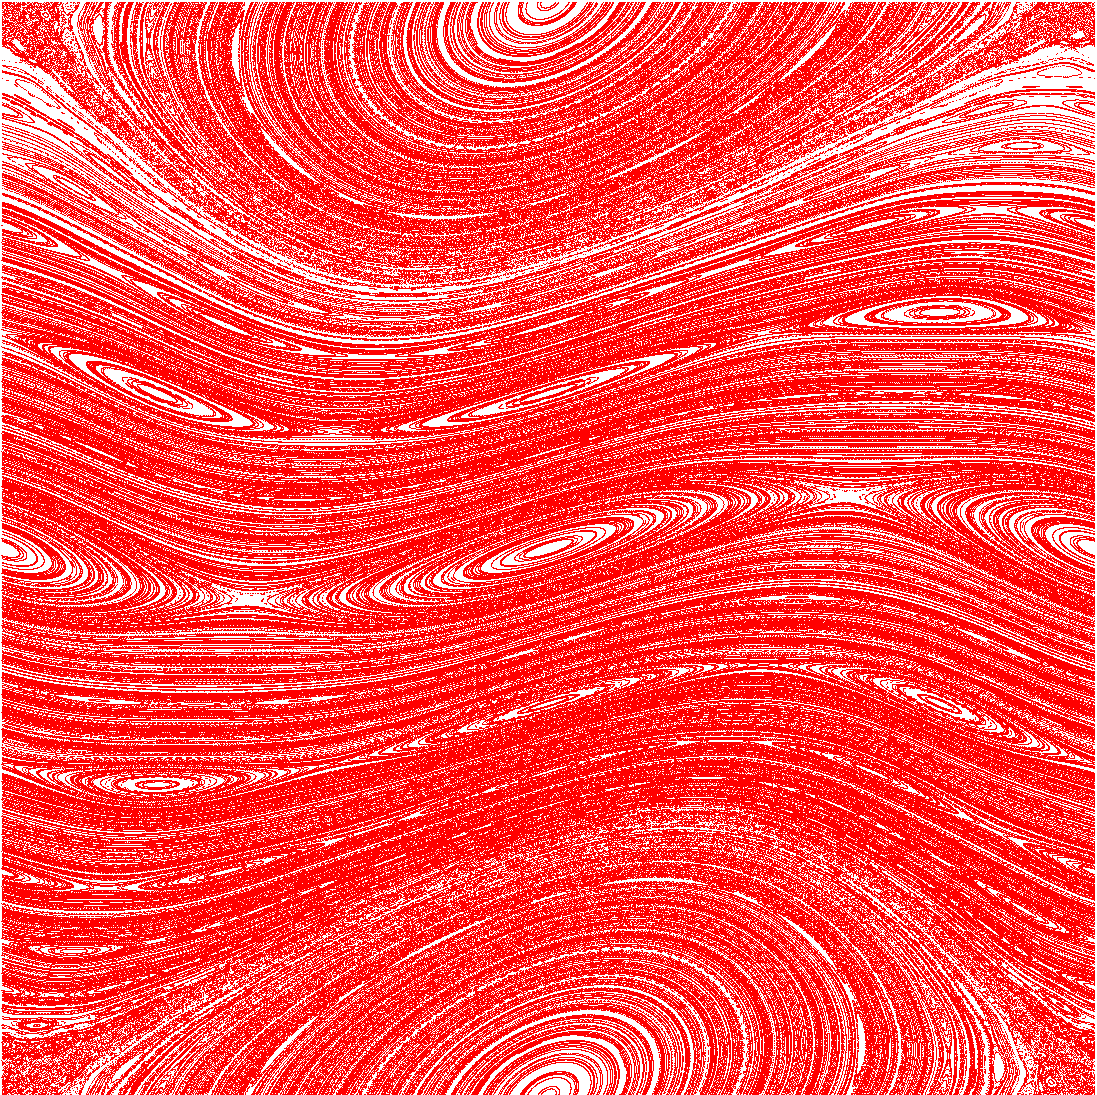
\includegraphics[scale=0.13,trim=0cm 0cm 0cm 0cm]{ch1_litrev/k_0_6.png}
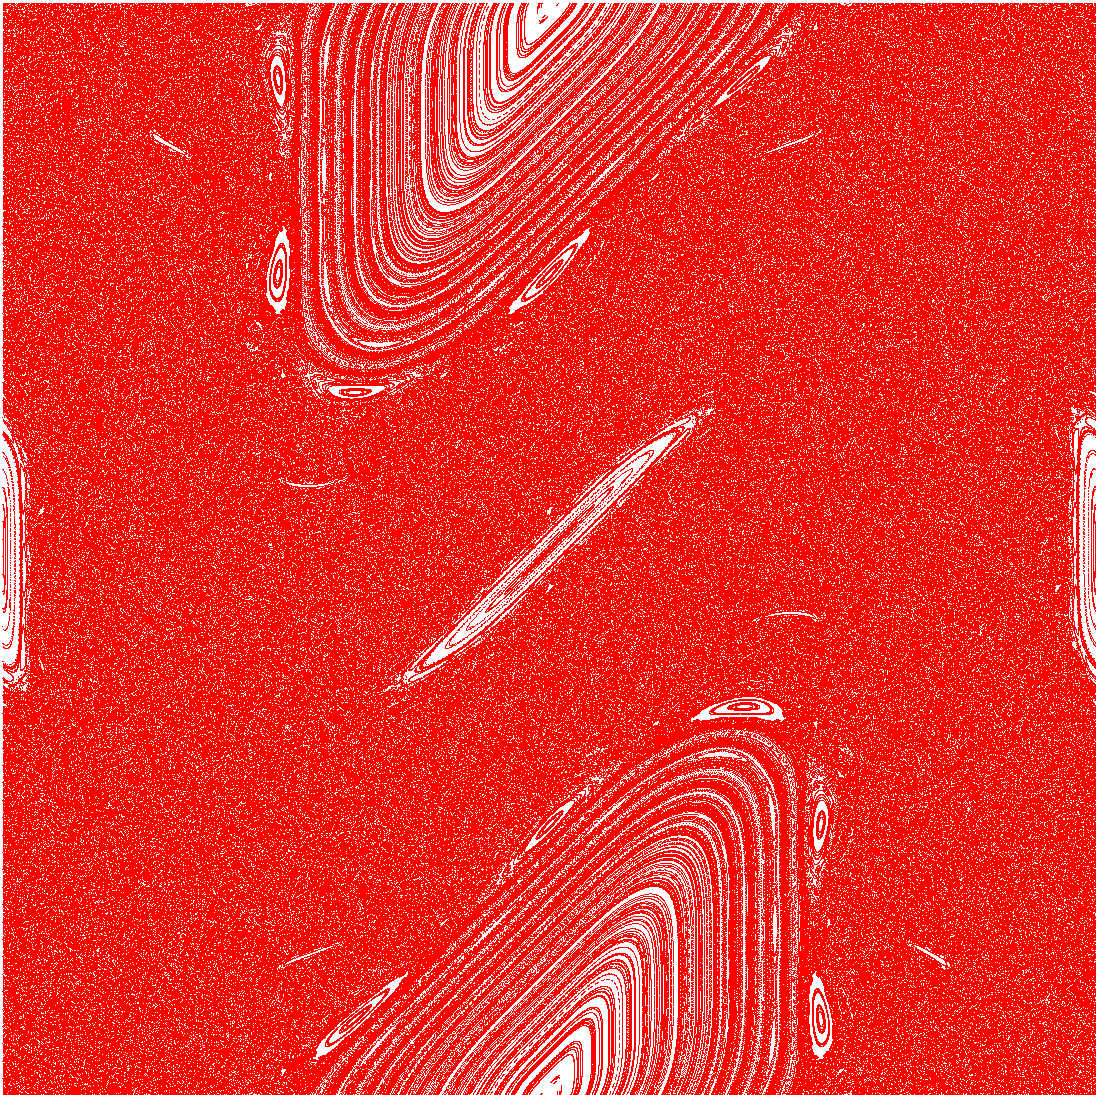
\includegraphics[scale=0.13,trim=0cm 0cm 0cm 0cm]{ch1_litrev/k_2_0.png}

\includegraphics[scale=0.13,trim=0cm 0cm 0cm 0cm]{ch1_litrev/k_12_0.png}
\caption{Images left to right represent phase space states of the classical kicked rotor using the standard map with increasing kicking strength, $K$. The left panel corresponds to $K=0.6$, still showing trajectories; the middle panel is for $K=2.0$, which shows chaos and 3 visible orbit regions; the right panel shows $K=12.0$ yielding a completely chaotic state.}
\label{fig:kickedrotor}
\end{figure}

One widely used model applied to understand such dynamics is that of the kicked rotor \cite{CT:Korsch_ajp_2008}. This model can be thought of as a particle rotating about a fixed point on a ring, receiving periodic kicks, the relative strength and sign of which depend upon the position on the ring. The variables in such a model are the momentum, $p$, which can take any value, and the angle, $\theta$, which is confined to values between 0 and 2$\pi$. The Hamiltonian describing such a system is given by
\begin{equation} \label{eqn:kickedrotor}
H = \frac{p^2}{2m} - K\cos(\theta)\displaystyle\sum_{n=-\infty}^{\infty}\delta(t-n\tau),
\end{equation}
where $K$ represents the kicking strength, and $\delta$ is the Dirac delta function, with $\tau$ being the kicking period. This type of system has been extensively used to understand both classical and quantum chaotic behaviour \cite{CT:Ulah_thesis_2012}. Examples for the trajectories for differing kicking strengths, $K$, are given in Fig. \ref{fig:kickedrotor}. It is easy to see that low kicking strengths give closed orbits, whilst an increase in kicking strength allows the system to enter a globally chaotic regime. The images in the chaotic regime demonstrate the area-filling property of the Poincar\'e section in phase--space.

A related system offering similar behaviour is the delta kicked harmonic oscillator, which modifies the Hamiltonian defined by Eq. \eqref{eqn:kickedrotor}, to include an additional harmonic potential. The resulting Hamiltonian is
\begin{equation}\label{eqn:deltaharmosc}
H = \frac{p^2}{2m} + \frac{m\omega^2 x^2}{2} - K\cos(kx)\displaystyle\sum_{n=-\infty}^{\infty}\delta(t-n\tau),
\end{equation}
where $\omega$ is the frequency of the harmonic potential, and $k=2\pi/\lambda$ is the wavenumber of the periodic potential.  This model can be thought of as a classical particle in a harmonic potential, oscillating and receiving periodic kicks with the strength and sign dependent upon the position within the potential. Gardiner \cite[chap. 4]{THS:Gardiner_2000} discusses this model, and the resulting chaotic behaviour for the classical case and for the quantum case. Variation of the kicking strength and period leads to a variety of interesting dynamics, and the onset of chaos can be observed as the kicking strength increases.

\subsection{Chaos in quantum systems}
The statements characterising chaos given in Section \ref{ss:chaotic} are applicable to classical systems only. One significant difference is that the sensitivity to initial conditions is no longer given due to the unitary nature of the quantum operators \cite{CT:Schack_pre_1996,CT:Gardiner_pra_2000}. The connection between classical chaotic behaviour and quantum mechanics, therefore, remains to be understood as the correspondence principle, given by Bohr, states that quantum dynamics has to reproduce classical dynamics in certain limits. However, classically chaotic systems do not show a quantum counterpart. The hypersensitivity to initial conditions does not appear in quantum systems, and quasiperiodic quantum systems can have a fully chaotic classical equivalent system \cite{CT:Jensen_nat_1992}. As such, the term ``quantum chaos'' has come to refer to
quantum systems which can be described by a Hamiltonian exhibiting chaos in a classical setting. The quantum delta kicked harmonic oscillator, previously described for classical systems, has been studied for its ability to generate chaotic dynamics in works given by Daly \cite{THS:Daly_1994}, Gardiner \cite{THS:Gardiner_2000}, and Kells \textit{et al}. \cite{CT:Kells_pre_2004}. Given the requirement of non-integrability to observe chaotic dynamics, it is worth noting that in the limit where the Schr\"{o}dinger equation is valid the system can be integrable due to its linear nature \cite{THS:Gardiner_2000}. The quantum delta-kicked harmonic oscillator dynamics can be examined by replacing the classical conjugate variables, $(x,p)$, of the Hamiltonian Eq. \eqref{eqn:deltaharmosc}, with their quantum operators, $(\hat{x},\hat{p})$, as
\begin{equation}\label{eqn:hamiltonian_qkick}
\hat{H} = \frac{\hat{p}^2}{2m} + \frac{m\omega^2 \hat{x}^2}{2} - K\cos(k\hat{x})\displaystyle\sum_{n=-\infty}^{\infty}\delta(t-n\tau).
\end{equation}
The dynamics in such a quantum system can be examined using similar tools as the ones presented for classical systems, such as phase-space visualisation. Obtaining a phase-space representation of the wavefunction is, however, not as straightforward as in the classical case. A common method for this involves calculating the Wigner quasiprobability function from the wavefunction.

Experimentally realisable systems that can exhibit such behaviour have recently become accessible, with the delta kicked rotor having been implemented in an optical and condensate system \cite{CT:Ullah_epjd_2012,CT:Lemos_natcomm_2012}. Such systems are, however, still rare. The extension of the above Hamiltonian to non-linear systems described by the Gross--Pitaevskii equation, rather than the linear Schr\"{o}dinger equation, opens up the possibility of observing interesting dynamics. Given that the area of quantum chaos is not as developed as that of classical chaos, the literature is not as well formulated, and tends to be more qualitative than quantitative, barring a few works. The use of Floquet theory is required to fully understand how to analyse periodic quantum chaotic systems, as it is a widely used method applied to describe the quantum behaviour \cite{CT:McCaw_thesis_2005}. Mapping a system onto the Hamiltonian as, for example, the one given by Eq. \eqref{eqn:hamiltonian_qkick}, would provide a way to realise a system that can yield observable chaotic behaviour. For this reason, the proposal given in Section \ref{sec:prelim} will discuss using this Hamiltonian as an integral part of my PhD thesis research.
 % Import your chapters here
        %\section{Thesis proposal}\label{sec:prelim}

\subsection{Project definition}
%I shall begin by restating many of the points covered throughout this literature review: The realisation of condensates was was first given in 1995, following prediction nearly 60 years previously. The behaviour of such systems saw much interest, with theoretical and experimental work seeing a significant rise since this date. One of the properties of condensates, the superfluid nature, received a large degree of attention, with many investigating the nature of quantised vorticity. Approaching the fast rotation limit allows these vortices to enter a crystalline lattice state, analogous to the Abrikosov lattice seen with type-II superconductors subjected to a static magnetic field. This mean-field quantum Hall regime remains predictable using the Gross--Pitaevskii equation, as it is still a weakly correlated state for a range of values beneath the fast-rotation limit. The use of optical lattices with condensates allows for the creation of strongly correlated states, giving a transition between Mott insulator and superfluid regimes by varying lattice intensity. Studies combining vortex lattices and optical lattices have shown transition from Abrikosov to pinned lattice state. Given the fluid superfluid nature of condensates it is possible to study chaos in the quantum regime. The kicked harmonic oscillator lends itself as an ideal model to attempt an understanding of chaos in quantum systems, and has been demonstrated as such.
As part of my PhD I intend to investigate the dynamical behaviour of Bose--Einstein condensates within the fast-rotation limit. With the rotation frequency approaching the trapping frequency of the condensate, the appearance of an Abrikosov (triangular) lattice of vortices in the condensate is expected. This is similar to the type of behaviour observed in type-II superconductors subjected to an applied magnetic field \cite{QM:Abrikosov_jpcs_1957}. With the condensate ground-state having an Abrikosov lattice of vortices, the goal will be to investigate quantum dynamical behaviour in this mean-field quantum Hall regime, with an investigation into chaotic dynamics. This will be carried out by treating the system as a delta-kicked quantum oscillator, where a periodically pulsed optical lattice, whose structure is matched to that of the vortex lattice, is doing the kicking. The plan is to treat the vortex as an effective particle through which the (potentially chaotic) dynamical behaviour may be observed. The Hamiltonian of this system can be mapped to that of the delta-kicked harmonic oscillator Hamiltonian, and will allow for a means to describe the resulting dynamics using an analytical  approach.
%The delta kicking shall be from an intense Gaussian laser field, applied to the vortex position at timescales shorter than the condensate dynamics. However, dealing with a single vortex and single narrow laser is possible, more experimentally realisable, and useful information may be obtained from the use of a large collection of vortices, such as the Abrikosov lattice. The subjecting laser field shall thus be given as that of an optical lattice, with structure matching that of the vortex lattice.

Due to the complex nature of this proposed system, a significant degree of computation will be required. Following on from the methods given in Section \ref{sec:numerics}, one way to perform the large computations required are through use of graphics processing units (GPU). I have previously worked on developing an application for the numerical solution of a fully three-dimensional Schr\"{o}dinger equation in waveguides using GPUs \cite{AO:Morgan_ORiordan_pra_2013}, and I have used this as the basis for the study proposed. I have further modified the developed code to deal with the non-linearity arising from the Gross--Pitaesvkii equation \eqref{eqn:gpe_rotation}, and to account for angular momentum. The resulting code was published under an open-source LGPLv2 license, and named ``GPUE'' \cite{NUM:gpue}. Generalisation of this code will allow more complex quantum systems to be examined, and so far has been shown to achieve results in substantially less time than competing implementations.

%For a thorough understanding of the numerically obtained results, more complex analytics will be considered and applied. For this the Wigner quasi-probability function will be calculated, to allow observation of the phase-space dynamics of the system. I will also apply Floquet theory to this periodic system, which will allow the derivation of analytical results in certain limits. 
%Once the code to determine the ground-state under large rotation is developed, the preparation of a vortex lattice with any specified number of vortices is expected to be numerically possible. Such a system may then be pulsed via briefly applied external potentials. Considering the use of a triangular optical lattice, wherein the lattice spacing is equivalent to the inter-vortex spacing of the condensate, a 1:1 mapping of the optical lattice to the vortex lattice can be achieved within a certain condensate radius. The goal of my project is to create a system in which behaviour akin to that of the delta-kicked quantum oscillator can be observed and to study the potentially chaotic dynamics. Treating the vortex as an effective particle, and the optical lattice potential as a delta perturbation in time, it may be possible to observe signatures of chaos for topological excitations. %Quantification of quantum chaos in experimentally realisable systems, such as superfluid Helium, is a challenging feat \cite{CT:Kobayashi_pra_2007}. The use of dilute condensates instead of superfluid Helium offers much greater ease in observing phase and density, and as such these systems may offer more insight into, and showcasing of the dynamics that can be expected to occur.

To effectively study this system, it will be necessary to obtain a thorough understanding of both classical and quantum chaos for 
Hamiltonian systems. Properties of the system will be analysed, with phase-space methods, such as calculating the Wigner function, which will provide information about the system dynamics \cite{CT:Gardiner_pra_2000}. It will be necessary to calculate the Wigner function for each variation of the condensate system parameters, and further indepth studies using Floquet analysis will be necessary for effective characterization of the observed behaviours \cite{CT:chu_physrep_2004,CT:McCaw_thesis_2005,CT:Gardiner_thesis_2000,CT:Kells_pre_2004}.

\subsection{Overall aims}
For successful completion of this project the following goals are outlined.
\begin{itemize}
	\item Generate a large, stable vortex lattice using a Bose--Einstein condensate within the MFQH regime.\vspace{-1em}
	\item Generate dynamical simulations of BECs using a periodically pulsed optical lattice matched to vortex lattice.\vspace{-1em}
	\item Track the motion of individual vortices in position space, and characterise dynamical behaviour observed.\vspace{-1em}
	\item Analyse the behaviour of the system in phase-space using the Wigner function of the resulting dynamics.\vspace{-1em}
	\item Apply Floquet theory to the system, and infer information about the observed behaviour from the results.
\end{itemize}
Experiments to observe chaotic behaviour in the quantum regime are rare, and the realisation of this type of system should allow for the first of its kind to observe chaos in a system of well-ordered topological excitations. Given recent experimental progress in the area of trapping, cooling, rotating and controlling Bose--Einstein condensates, the proposed system should be realisable with currently available experimental techniques.
The required techniques for theoretically performing this body of work will be described below.

\subsection{Methods and techniques}
\subsubsection{Creating a vortex with phase imprinting}
As a precursor to this proposal, I have performed preliminary work during my time in the Busch unit to investigate the behaviour of condensates with differing numbers of
vortices, and subjected to a short external pulse. Initially, the behaviour of a condensate with a low number of vortices (0,1,2) was examined. 
Numerical integration of the two dimensional Gross--Pitaevskii equation in imaginary time in the co-rotating frame allowed for the
determination of the ground-state in the absence of the perturbation. A predefined winding number, corresponding to the number of vortices required, was applied by multiplication of an appropriate phase with an initial Gaussian guess for the wavefunction guess, and evolved in imaginary time. After that, the resulting numerical ground-state solution was perturbed by kicking it with an additional Gaussian phase pattern, representing a laser pulse (kick), and he system was evolved in real time. A Gaussian phase is
known to give rise to breathing modes in the condensate \cite{BEC:Kimura_pra_2002}, as the velocity of the condensate atoms is given by the 
gradient of its phase. With a kick of large amplitude, the atoms with sufficiently steep phase gradient will move at a greater velocity than those at the
edges or the centre of the Gaussian pulse. As a result, the faster moving atoms will overtake those in the slower moving regions, and due to the
coherent nature of the condensate, matter-wave intereference fringes were observed. From this observation, it is clear that the condensate
under these conditions behaves as an interferometer. With the presence of more than a single Gaussian pulse more complex interference 
patterns can develop and any inhomogeneities in the trapping potential will give rise to a non-symmetric fringe pattern, which may in turn be used to determine the quality of the trap, or the topology of nearby structures. Example results are shown in Fig. \ref{FIG:bec_fringe}.
\begin{figure}[tb]
\begin{center}
	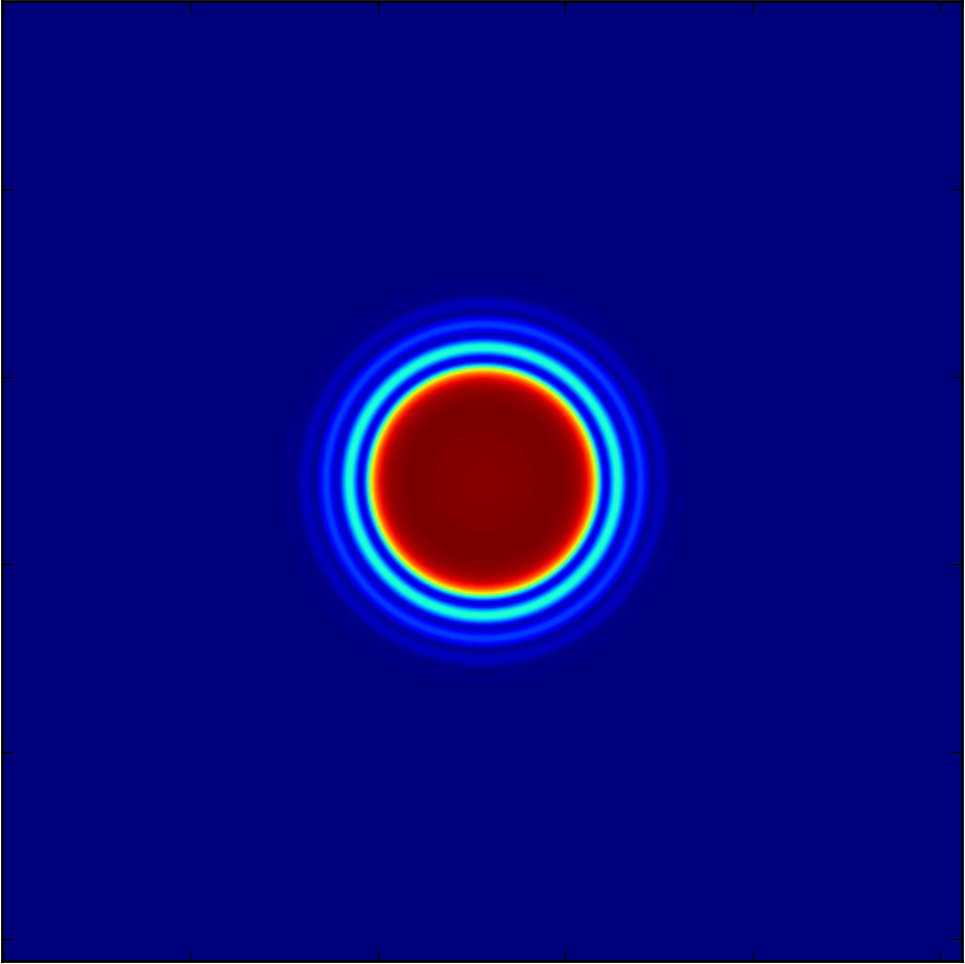
\includegraphics[trim=10cm 10cm 10cm 10cm, clip, scale=0.25,width=3cm]{ch1_litrev/symmetric_guassian_no_vortex_expansion.png}\vspace{0.1em}
	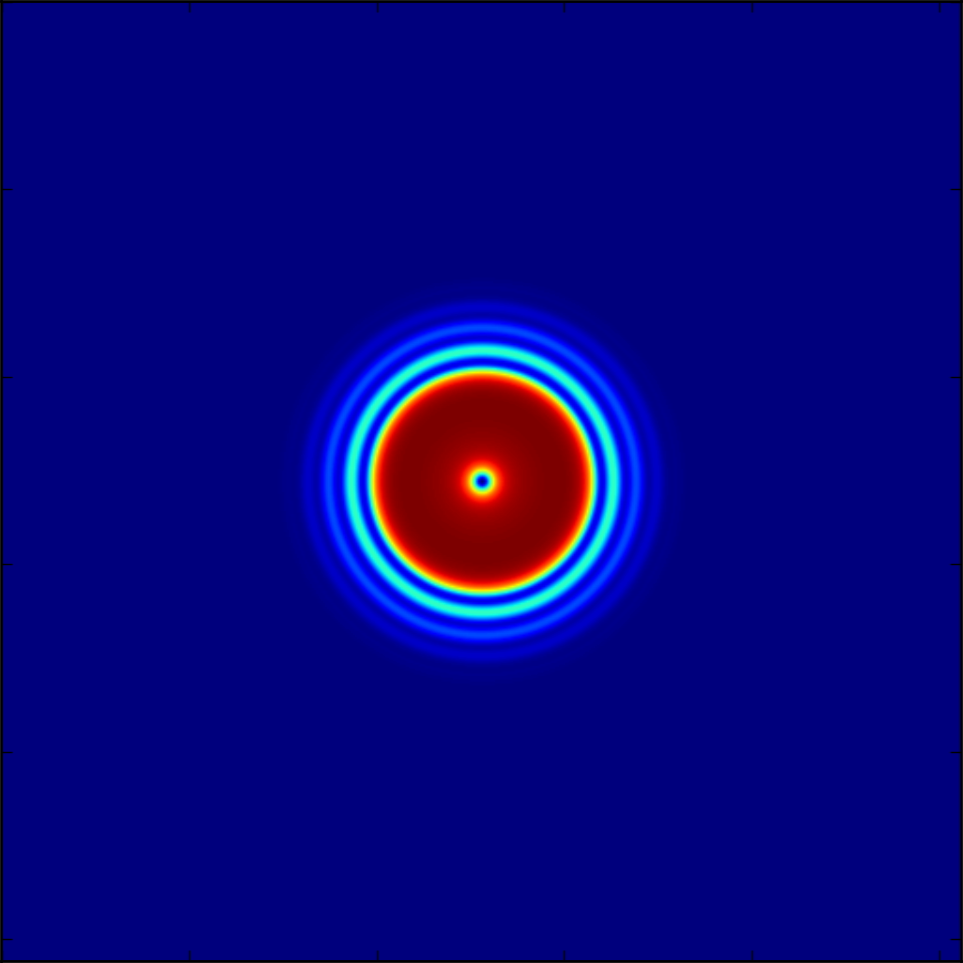
\includegraphics[trim=10cm 10cm 10cm 10cm, clip, scale=0.25,width=3cm]{ch1_litrev/symmetric_gaussian_centre_1vortex_fringe_1stexpansion.png}
	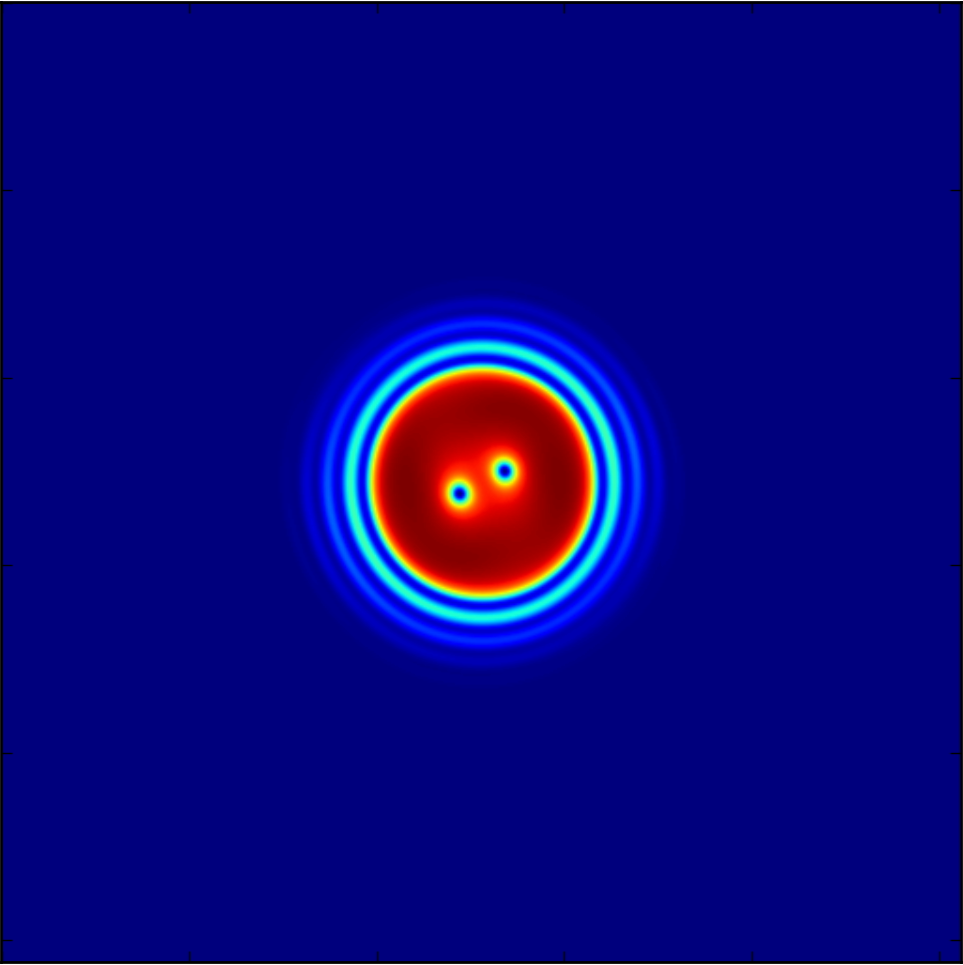
\includegraphics[trim=10cm 10cm 10cm 10cm, clip, scale=0.25,width=3cm]{ch1_litrev/rotating_2vortex_gaussian_centre_1stexpansion.png}
	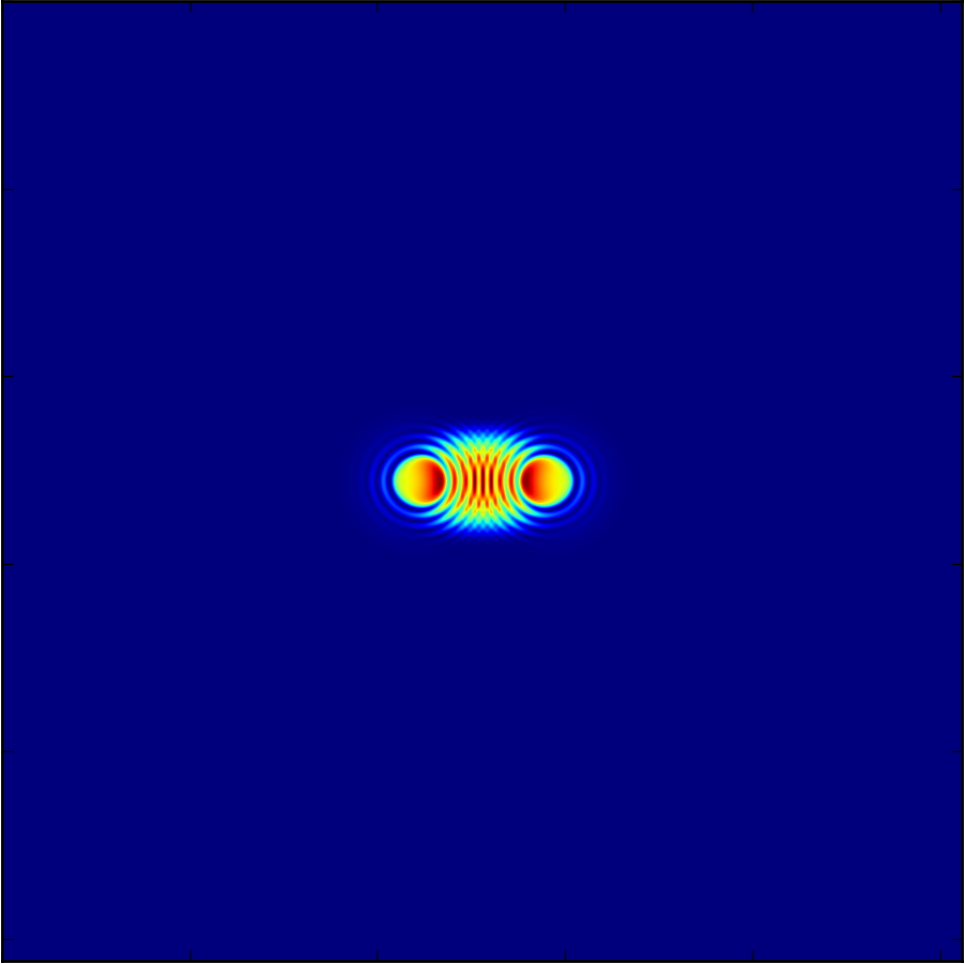
\includegraphics[trim=12cm 12cm 12cm 12cm, clip, scale=0.25,width=3cm,height=3cm]{ch1_litrev/assymetric_0vortex_gaussian_left_right_higher_power.png}
	
	
	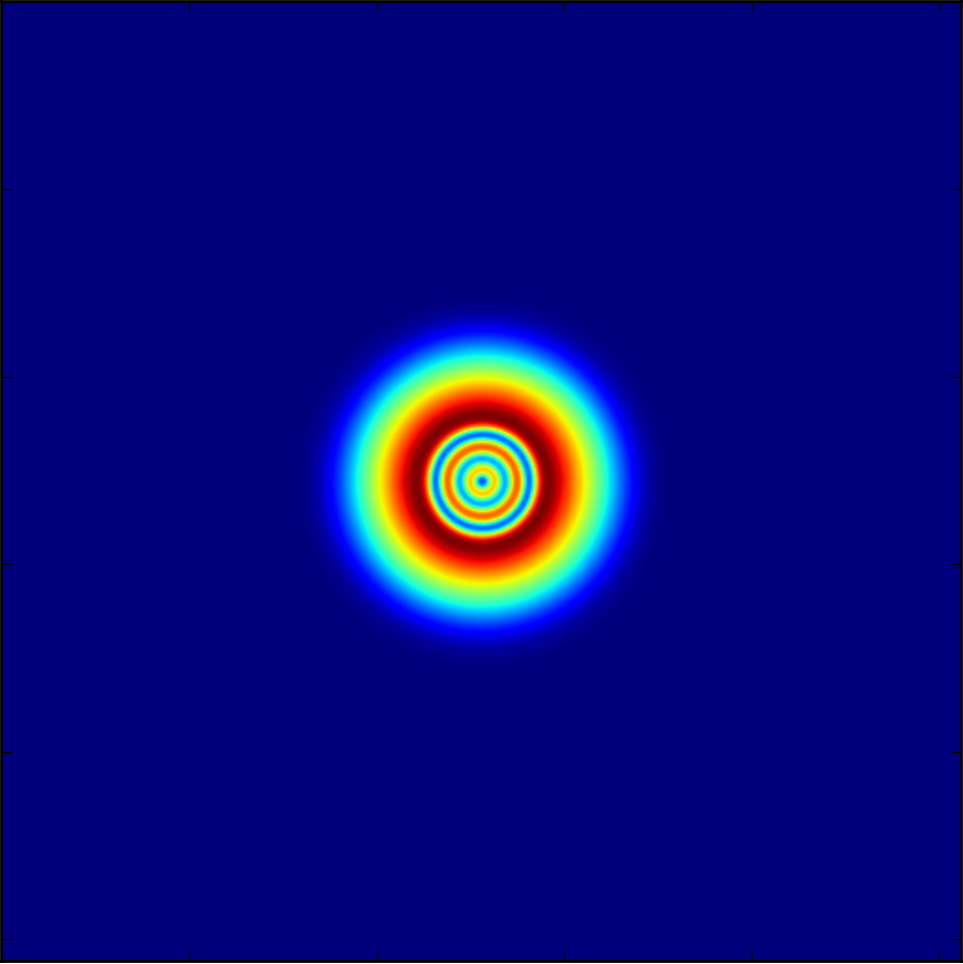
\includegraphics[trim=10.1cm 10cm 10.1cm 10cm, clip, scale=0.25,width=3cm]{ch1_litrev/symmetric_guassian_no_vortex_contraction.png}
	\includegraphics[trim=10.1cm 10cm 10.1cm 10cm, clip, scale=0.25,width=3cm]{ch1_litrev/symmetric_gaussian_centre_1vortex_fringe_1stcontraction.png}
	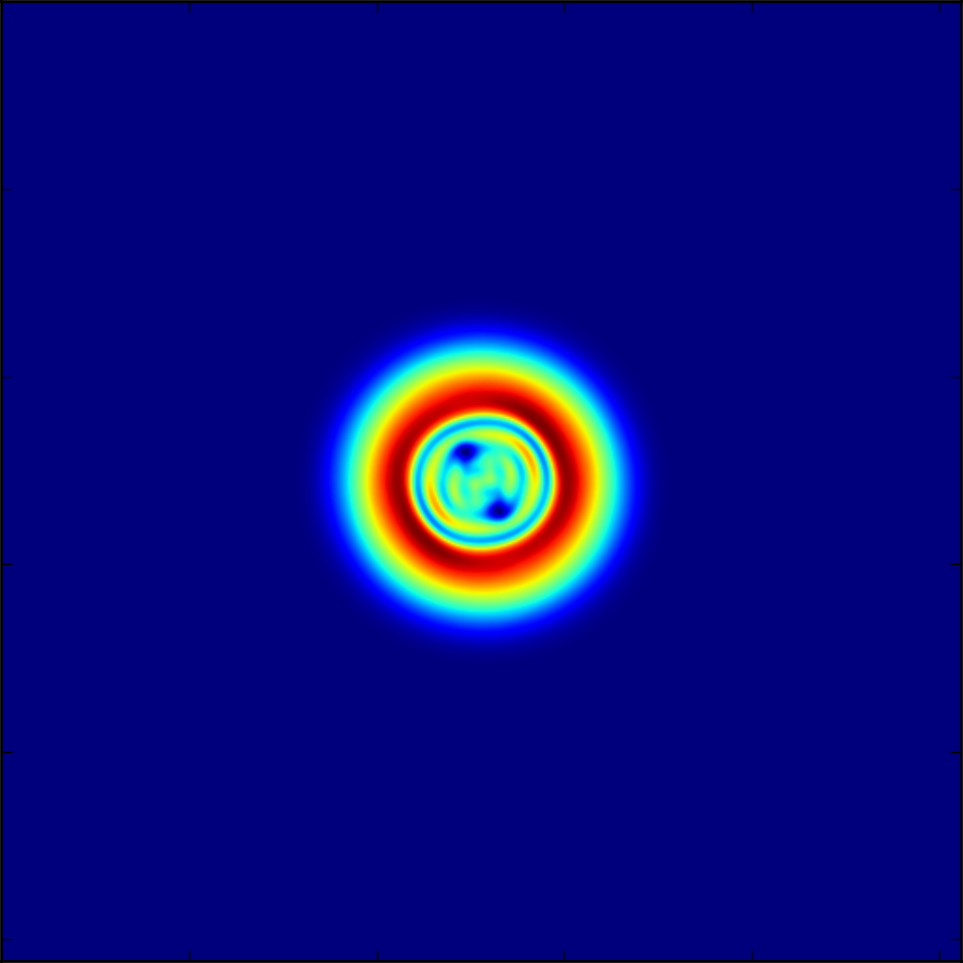
\includegraphics[trim=10.1cm 10cm 10.1cm 10cm, clip, scale=0.25,width=3cm]{ch1_litrev/rotating_2vortex_gaussian_centre_1stcontraction.png}
	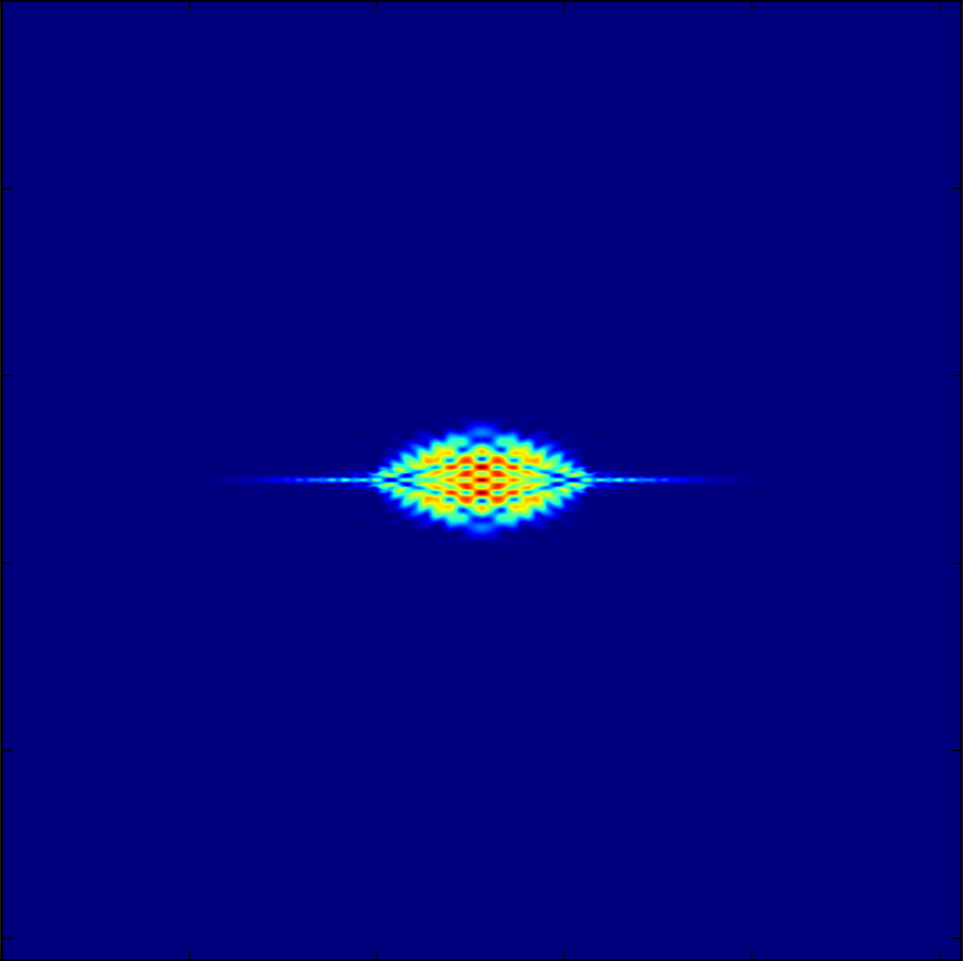
\includegraphics[trim=12cm 12cm 12cm 12cm, clip, scale=0.25,width=3cm,height=3cm]{ch1_litrev/asymetric_novortex_dual_gaussian.png}
	%\includegraphics[trim=10.1cm 10cm 10.1cm 10cm, clip, scale=0.25,width=3cm]{images/symmetric_gaussian_centre_1vortex_fringe_1stcontraction.png}
\end{center}\vspace*{0pt}\caption{Sample results of BECs with varying number of vortices subjected to different phase imprinted patterns. Images are paired top and bottom, at different stages of evolution. From left to right the examined systems are: (i) harmonically trapped condensate with no vortex plus a Gaussian phase in centre; (ii) harmonically trapped condensate with a single vortex plus a Gaussian phase in centre; (iii) harmonically trapped condensate with two vortices plus a Gaussian phase in centre; (iv) anharmonically trapped condensate with no vortex plus two Gaussian phase patterns on opposite sides of condensate\vspace*{-10pt}}\label{FIG:bec_fringe}
\end{figure}

\subsubsection{Creating a vortex lattice}
At low values of the rotation ($0 \leq \Omega \leq 0.49\omega_{\perp}$) the condensate can support a small number of vortices, which when evolved
in imaginary time will form a uniform structure. Increasing the rotation frequency further ($0.5\omega_{\perp} \leq \Omega \leq 0.89\omega_{\perp}$) allows the condensate to support a much larger number of vortices, which can arrange themselves into a lattice pattern. At values approaching the limiting frequency the vortices should order into a large Abrikosov lattice pattern, similar to what
is observed in type-II superconductors. Starting with a large winding number for the phase imprint pattern, the resulting initial guess is evolved in imaginary time, and values approaching the fast rotation limit were chosen. Figure \ref{fig:close_to_abrikosov} shows an example of the condensate under fast rotation, assuming an initial winding of the order 100.
 \begin{figure}[tb]
 \centering
 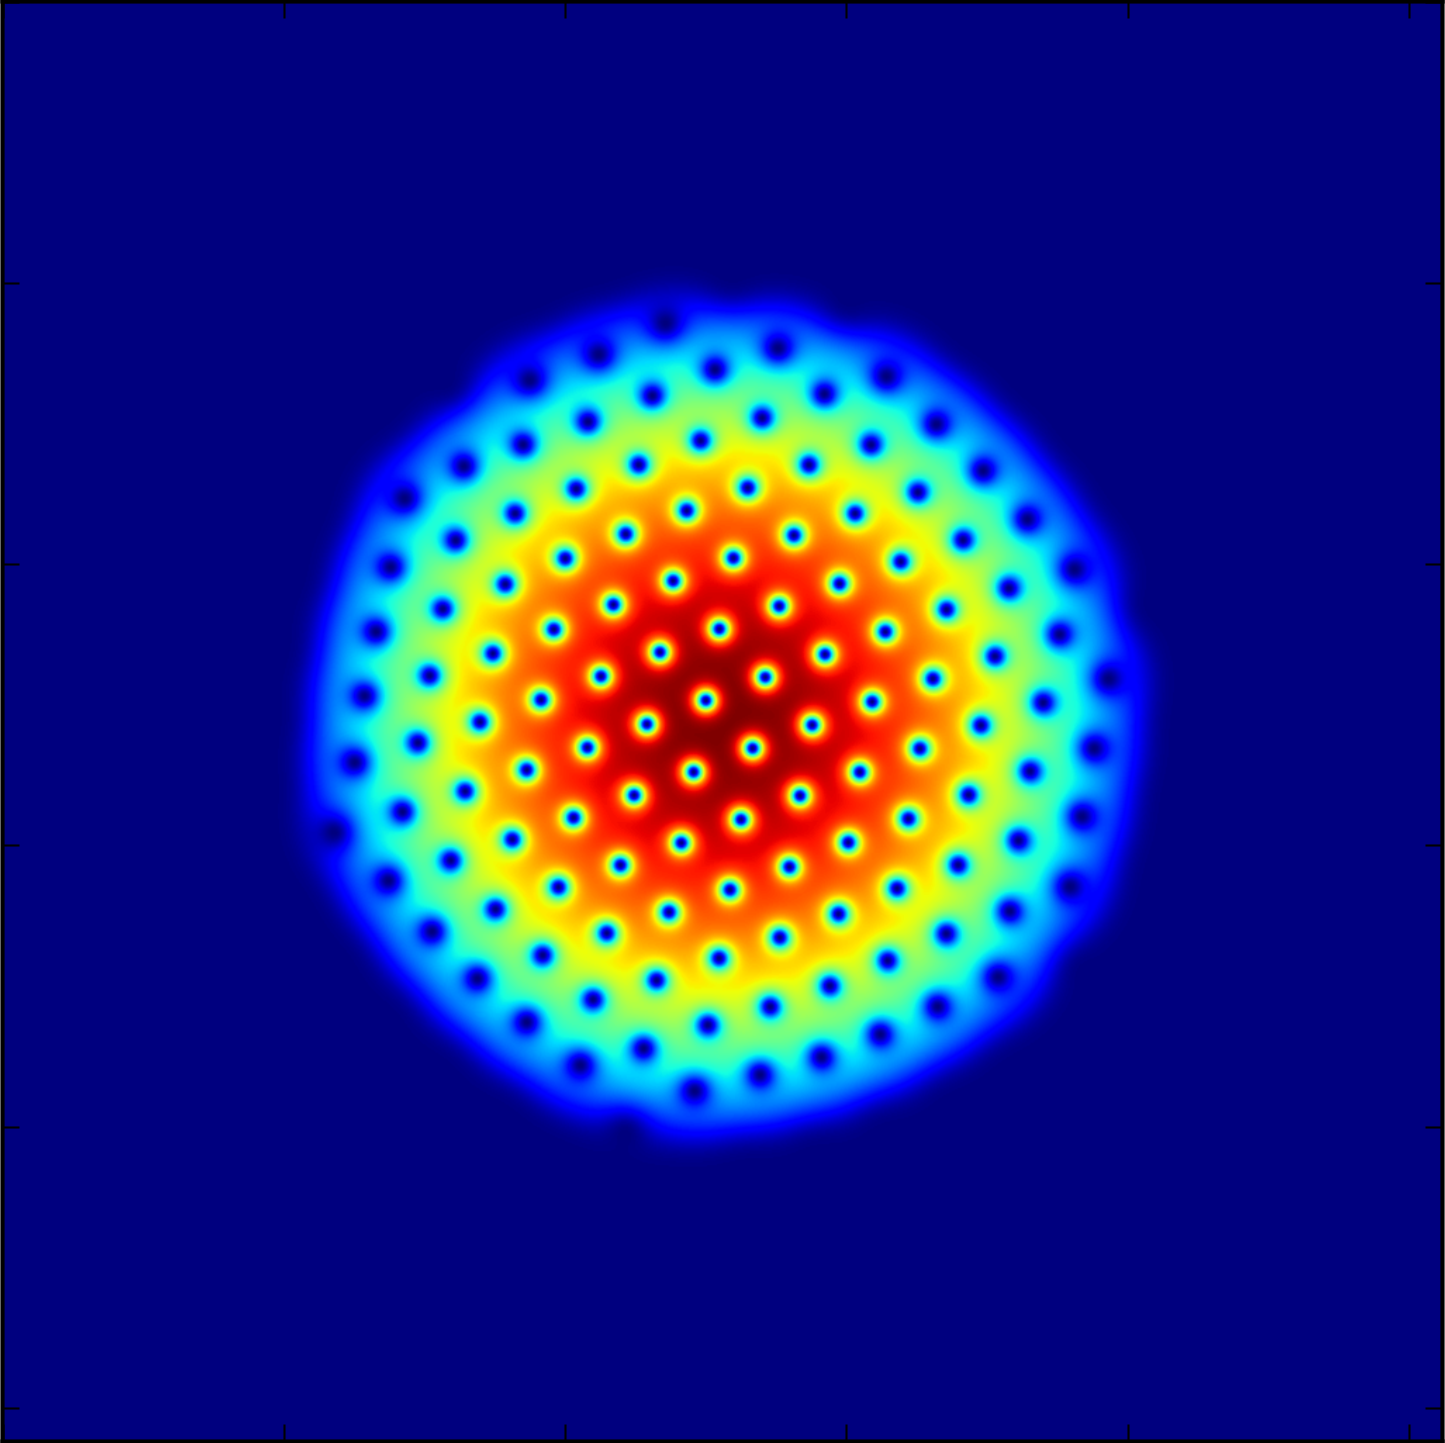
\includegraphics[scale=0.085]{ch1_litrev/wfc_19900000.png}
  \includegraphics[scale=0.085]{ch1_litrev/phi_19900000.png}
  \caption{Images show the ground-state of a condensate rotating at a frequency of $\Omega=0.9\omega_{\perp}$. Even though the Abrikosov lattice is clearly visible, a number of imperfections can be seen in the vortex alignment. Left image shows density, right image shows the phase.}
  %, evaluated at a timestep of $2\times 10^{-6}$ over a grid of $2^{10}\times 2^{10}$
  \label{fig:close_to_abrikosov}
 \end{figure}
To simulate this type of system careful consideration of the angular momentum term in the Hamiltonian must be taken. Initial results have been obtained through use of the GPUE codes that I have developed. However,  the implemented algorithm fails to botain a stable vortex lattice at large rotational frequencies, and so will require an alternative treatment of the system to generate the required state.

\subsubsection{Triangular optical lattice pattern}
For the optical lattice potential, three retroreflected laser fields are considered, giving rise to plane-waves oriented at 0, $\pi/3$ and $2\pi/3$. The resulting fields are defined as 
\begin{equation}\label{eqn:lattice_potential_tri}
V_{opt} = V_0\left[\cos^2\left(k\frac{x-\sqrt{3}y}{2} \right) + \cos^2\left(k\frac{x+\sqrt{3}y}{2} \right) +\cos^2\left(ky\right)\right],
\end{equation}
where $V_0$ is the amplitude of the optical lattice, and $k$ is the wavevector, given by $k=2\pi/\lambda$. A sample resulting optical lattice potential is shown in Fig. \ref{fig:optical_lattice}. The optical wavelength and position can be precisely controlled, even though it is an experimentally challenging task. Given the fine control over condensate parameters, matching the optical lattice to the vortex lattice structure is expected to be experimentally realisable, albeit with cutting edge techniques \cite{Vtx:Tung_prl_2006}.
\begin{figure}
\centering
	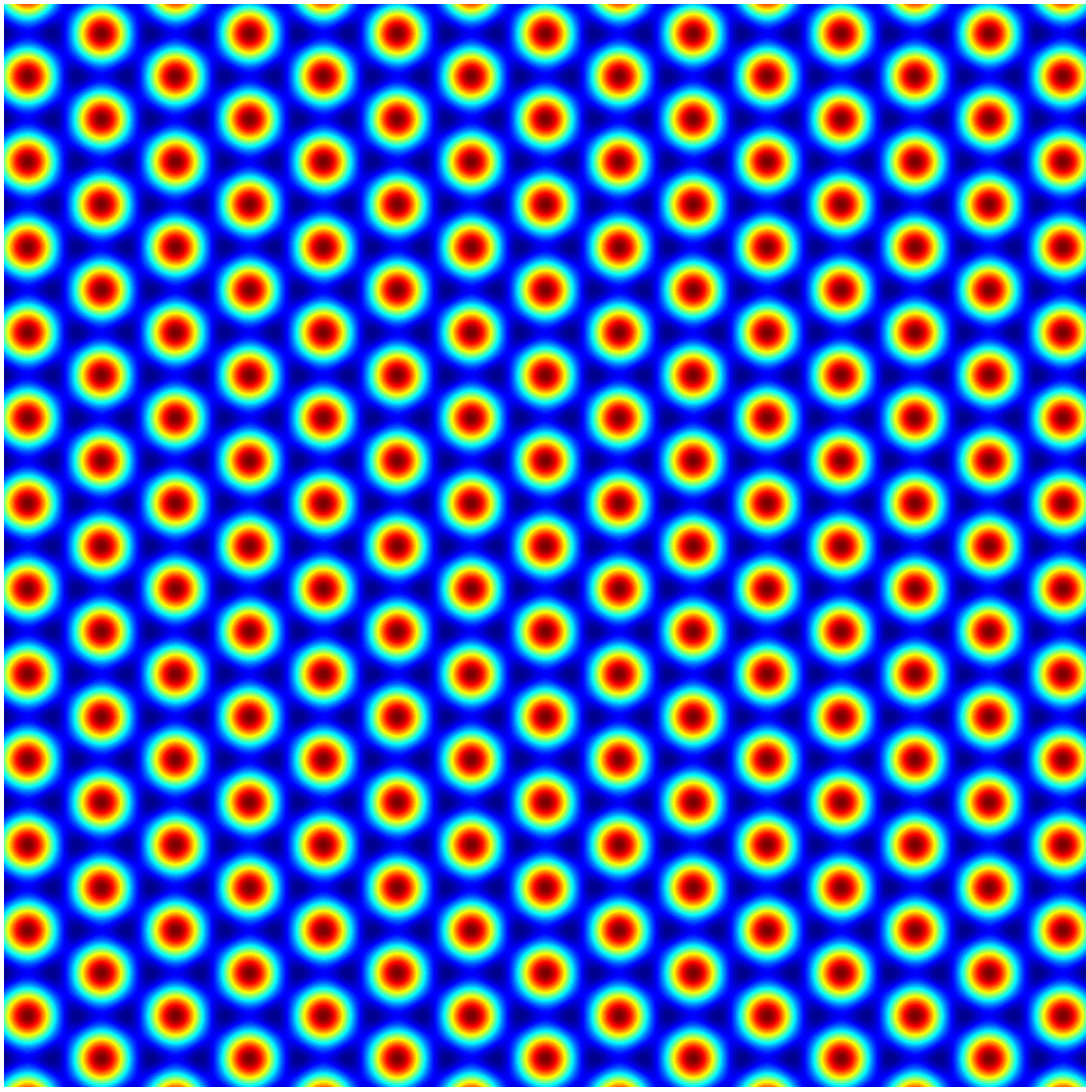
\includegraphics[scale=0.2]{ch1_litrev/opt_latt_g.png}
	\caption{The above image shows a triangular optical lattice potential pattern. This pattern will be adjusted to match the Abrikosov lattice pattern of the condensate in the fast-rotation limit.}\label{fig:optical_lattice}
\end{figure}
To use this optical lattice to generate the expected dynamics in the simulation it will be applied during the real-time evolution. This can be allowed by summing with the trapping potential for an instantaneous pulse of timescale equal to the time-step, or can be applied directly to the condensate phase.

\subsubsection{Delta kicked harmonic oscillator}
Using the Abrikosov lattice pattern with the triangular optical lattice potential we can map this system to the delta-kicked harmonic oscillator, presented in Section \ref{sec:chaos}. In the fast rotation limit, with an Abrikosov lattice pattern of vortices, the lattice undergoes a solid-body rotation. Given that the Abrikosov lattice is a triangular lattice pattern, the system has six-fold rotational symmetry, corresponding with a rotation of $\pi/3$ radians. Thus, a kick applied after a rotation through multiples of this angle will provide a periodic pulsing. The time to rotate through this angle will give the required period, $\tau$, of the system. The amplitude of the optical lattice pattern
will yield the kicking strength, $K$. It is expected that after a yet undetermined number of initial kicks the vortices will start interacting and move from an Abrikosov geometry. After this, all vortices will feel subsequent kicks with a strength dependent upon distance from the maxima and minima of the optical lattice, and should yield some chaotic dynamics. The chaotic dynamics of the system will be investigated by observing the motion of the vortices after a variable total number of kicks, choice of kicking period, lattice size, kicking strength, and a range of interaction strengths for the condensate. Further dynamical behaviour may be determined by calculating the Wigner distribution of the resulting wave-function, and also by analytical analysis using a Floquet theory approach.

\subsection{Significance of proposed work}
The extension between classical and quantum systems remains to be understood. At the classical--quantum limit, the observation of chaos offers a way to gain some insight into processes that may occur. Currently there have been no studies of quantum chaos in systems of topological excitations. Undertaken this project would be the first into investigating such behaviour, and as a result many interesting new physics may be observed. Characterisation of the chaotic behaviour observed in this type of system also will allow for comparative works between the classical and quantum cases. This is a newly developing area of investigation, and the use of condensate use investigating chaotic behaviour has seen few experimental realisations to date. The outlined set-up would allow for a highly controllable system to be subjected to a periodic perturbation relatively easily, mapping it well to the kicked harmonic oscillator. The resulting numerical routines developed should allow for a variety of physical phenomena to be investigated in much shorter timescales compared to currently available methods.

An extension of the work proposed in the project can go in many related directions. One possibility would be to study the transition from the mean-field regime to the strongly correlated (e.g. Mott insulator) regime. The Gross--Pitaevskii theory will no
longer be applicable in this regime, requiring a strict quantum mechanical treatment of bosons. However, it may be possible to formulate some
results for low atom numbers and low vortex numbers in reasonable timescales, again employing GPU computing.  Other possible areas of interest could be the behaviour of such condensates in an open setting, the study of finite temperature effects, differences arising from the dimensionality of the system, the effect of dipolar interactions in the condensate in the fast rotation limit with and without an applied optical potential, multicomponent condensates, and even coherent transport of the condensate in the fast rotation limit.
Another approach to the system discussed above is that of considering interacting charged particles. This can be done by considering each vortex in the lattice as a particle with unit charge, and the application of the delta kicking should lead to the same chaotic behaviour.

\subsection{Caveats}
As mentioned previously, all attempts to generate Abrikosov lattice states have been met with some difficulty. The previously
 used Fourier split-operator method \cite{Num:Bauke_cpc_2011} with Strang-splitting for improved numerical precision \cite{Num:Sanchez_parcomp_2008}, utilised in all previous work appears ill-suited for this system. What has been observed is the inability to effectively find a groundstate of the system
 under fast rotation, approaching the trapping-frequency limit. Some success has been achieved by running a long (several days) simulation (see Fig. \ref{fig:close_to_abrikosov}). However, such long simulation limit the progress which may be achieved. Given the numerical precision required to effectively resolve energies in these systems, new numerical methods must be investigated. One potential way to achieve simulations of condensates in the MFQH regime numerically is through use of the newly defined methods, such as those given by Bao \textit{et al}. and Ming \textit{et al} \cite{Num:Bao_siam_2013,Num:Ming_jcp_2014}. They have reported successful demonstration of numerical codes to investigate rotating condensate behaviour, without the associated difficulties in dealing with the angular momentum operator. It is not yet clear as to whether such methods are applicable to the MFQH regime, as the authors have not demonstrated more than tens of vortices.
 % Import your chapters here
\fi

%%%%%%%%%%%%%%%%%%%%%%%%%%%%%%%%%%%%%%
\newif\ifnumerics
\numericstrue
\ifnumerics
    \chapter{Numerics}
        \section{Fourier split-operator method}\label{sec:numerics}
For many of the works described previously, it is necessary to apply numerical techniques to obtain solutions. As the Gross--Pitaevskii
equation, given in Eq. \eqref{eqn:gpe}, is used in the majority of the literature cited, we will consider it as the basis for the following discussion. The Gross--Pitaevskii equation is a second order non-linear partial differential equation, and so very few exact solutions exist; the problem must often be tackled by a numerical approach. Though there are many ways to solve such a system numerically, (such as Crank-Nicholson, Trotter-Suzuki), the method I have chosen is the pseudospectral Fourier split-operator \cite{Num:Bauke_cpc_2011}.

If we consider a unitary evolution operator of the form
\begin{equation}\label{eqn:1}
\Psi(\mathbf{x},t+\tau) = \exp\left[ -\frac{iH\tau}{\hbar}\right]\Psi(\mathbf{x},t),
\end{equation}
where $H$ is the Hamiltonian, composed of momentum, potential, non-linear interaction, and rotation terms defined in Eq. \eqref{eqn:gpe}, we can solve for the wavefunction, and its resulting dynamics over a specified time-scale. However, due to error propagation resulting from numerical integration, it is instructive to employ methods that allow for the highest precision while providing results in useful timescales. To allow for this, care must be taken udring the implementation of such integration methods.  If we take the Hamiltonian, $H$, in terms of its components as a combination of position and momentum space functions we obtain
\begin{equation}\label{eqn:2}
{H} = {H}_{\textbf{r}} + {H}_{\textbf{k}} + {H}_{\textbf{L}},
\end{equation}
where we first neglect the angular momentum operator, ${H}_{\textbf{L}}$, and consider only the two other non-commuting parts ${H}_{\textbf{r}}$, containing the position operator, and ${H}_{\textbf{k}}$, containing the momentum operator. This way we can reduce the error in the numerical integration scheme by using 2nd order Strang-splitting as
\begin{equation}\label{eqn:3}
\exp\left[ -\frac{ i\left(\hat{H}_{\textbf{r}} + \hat{H}_{\textbf{k}}\right)\tau}{\hbar} \right] = \exp\left[- \frac{i\hat{H}_{\textbf{r}}\tau}{2\hbar} \right]\exp\left[-\frac{i\hat{H}_{\textbf{k}}\tau}{\hbar}\right]\exp\left[ -\frac{i\hat{H}_{\textbf{r}}\tau}{2\hbar}\right] + \mathcal{O}\left(\tau^2\right).
\end{equation}
The respective functions can be mapped to the Gross--Pitaevskii equations position, and momentum terms as
\begin{equation}
\hat{H}_{\textbf{r}} = V(\bar{x}) + g\vert\Psi(\bar{x},t)\vert^2\; \hspace{5em} \hat{H}_{\textbf{k}} = \frac{-\hbar^2}{2m}\nabla^2.
\end{equation}
%\hat{H}_{\textbf{L}} = \Omega L,
Following Bauke \textit{et al}. \cite{Num:Bauke_cpc_2011}, we can numerically solve this differential equation as
\begin{equation}
\Psi\left(\textbf{r},t+\tau\right) = \left[\hat{U}_{\mathbf{r}}\left(t+\frac{\tau}{2}\right) \mathscr{F}^{-1} \left[ \hat{U}_{\mathbf{k}}(t+\tau) \mathscr{F} \left[ \hat{U}_{\mathbf{r}}\left(t+\frac{\tau}{2}\right) \Psi\left(\mathbf{r},t\right) \right] \right] \right]  \\ + \mathcal{O}\left(\tau^3\right),
\end{equation}
where $\hat{U}_{r}=e^{-i\hat{H}_{r}(t)\tau/\hbar}$ is the time evolution operator in real space, $\hat{U}_{k}=e^{-i\hat{H}_{p}(t)\tau/\hbar}$ in momentum space,  $\mathscr{F}$ and $\mathscr{F}^{-1}$ are the forward and inverse Fourier transform respectively.

\begin{figure}
    \centering
    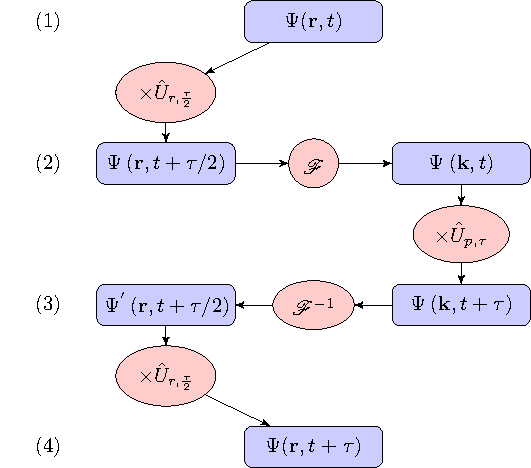
\includegraphics[]{./ch3_numerics/splitop}
    \caption{A single pass through the Fourier split-operator method.}
    \label{fig:num_splitop}
\end{figure}

%%% TO BE MOVED IN WITH PHASE ENGINEERING
Following \cite{BK:Pitaevskii_Stringari_2003} and taking the Madelung transform of the wavefunction given by Eq. \eqref{eqn:madelung}, the phase of the condensate may be specified as
\begin{equation}
\theta = \theta_c + \theta_i,
\end{equation}
where $\theta_c$ is the unperturbed condensate phase, and $\theta_i$ is the phase pattern to be imprinted. Thus, upon solving for the initial condensate phase, an additional phase pattern can be imprinted at any time by multiplying the wavefunction by the intended phase pattern. This is in line with the phase imprinting method, as previously introduced by Dobrek \textit{et al}. \cite{Vtx:Dobrek_pra_1999}. The underlying theory of the Fourier split-operator method for the Gross--Pitaevskii equation is given by Javanainen \textit{et al}. \cite{BEC:Javanainen_jphysa_2006}, showing how the choice of non-linearity and operator splitting affects the outcome of the method. The authors arrive at the conclusion that treating the non-linearity and potential terms together with the most current wavefunction definition yields results with an error magnitude that matches those obtained in the Schr\"{o}dinger Fourier split-operator case, indicating its applicability to this type of problem.
%%% TO BE MOVED IN WITH PHASE ENGINEERING

 \subsection{Time evolution}

We can write the wavefunction of a quantum system as a linear superposition of states as
\begin{equation}
     |\Psi \rangle = \displaystyle\sum\limits_{n} C_n |\Psi_n \rangle,
\end{equation}
where $| \Psi_n \rangle$ are a set of basis states for the system, with complex coefficients $C_n$. We next assume a unitary evolution operator of the form
\begin{equation}
    \mathscr{U}(t,t_0) = \exp\left(\frac{-i\mathcal{H}(t-t_0)}{\hbar}\right),
\end{equation}
where $\mathcal{H}$ is the Hamiltonian of the system. To time evolve our system from some time $t_0$ to a final time $t$ we apply the evolution operator to the wavefunction, giving
\begin{equation}
    \mathscr{U}(t,t_0)|\Psi \rangle = \displaystyle\sum\limits_{n} C_n \exp\left(\frac{-i{E_n}(t-t_0)}{\hbar}\right)|\Psi_n \rangle,
\end{equation}
where I have replaced the Hamiltonian operator with the energy eigenvalue of the $n$-th state. It follows from here that each state evolves at a different rate, proportional to its given eigenenergy. Higher energy states will oscillate faster than those of lower energy states. However, to make accurate predictions it is often necessary to deal with a single quantum state, such as the lowest lying state.

To create the initial state for the desired evolution the ground-state of the Hamiltonian must be determined as a first step. This can be achieved by evolving the system in imaginary time, causing all higher energy terms in an initial guess for the condensate wavefunction to decay to zero. This leaves the lowest energy state, which is the ground-state of the system. Taking the evolution operator, we apply a Wick rotation, rotating the time component through $\pi/2$ into the imaginary plane, as $t \rightarrow -it$. Applying this new evolution operator to the wavefunction gives
\begin{equation}
        \mathscr{U^{'}}(t,t_0)|\Psi \rangle = \displaystyle\sum\limits_{n} C_n \exp\left(\frac{-{E_n}(t-t_0)}{\hbar}\right)|\Psi_n \rangle.
\end{equation}
I have removed the complex term in the operator, which now takes the form of an exponentially decaying operator. When applied to the wavefunction all higher energy terms will decay at a rate faster than lower energy components. This process also causes a loss of probability density, and so the wavefunction must be renormalised after application. Through repeated application of this operator, and a renormalisation afterwards, the quantum system can converge to the groundstate. To begin, however, we must assume an intial guess for the wavefunction, which has some finite overlap with the lowest lying state.

As effective as this approach may be, the convergence to the lowest lying energy state becomes less effective as the computation approaches the expected value \cite{Vtx:Danaila_pra_2005}. Although many such methods exist, one that is well suited for this task is the previously discussed Fourier split-operator method. Due to the way the algorithm operates, it is essential to have a large and finely sampled grid in order to resolve both position and momentum of the wavefunction. A minimum grid-size on the order of $2^8$ in 2D for both $X$ and $Y$ dimensions is required, provided we are interested in trivial condensate dynamics.

Given that in the presence of large values of angular momentum, the condensate wavefunction will accomodate many vortices. To ensure a well ordered lattice, it is insufficient to numerically solve the GPE at the required rotation rate. Assuming an initial Gaussian guess, the large number of vortices will enter the condensate from the edge and compete for lattice sites to form the expected Abrikosov pattern. Thus, to overcome this issue, following the groundstate of the condensate with a ramp of the rotation rate is often necessary. This is essentially adiabatic evolution during imaginary time, and for all required rotation rates of the condensate we get a vortex lattice ground-state.

An implementation of this method is a straight-forward process using MATLAB, and has been performed for the purpose of this study. However, due to the large computational overhead required to time-evolve such a system, the procedure takes a long time to simulate the system at the required degree of precision. Therefore, it is necessary to further develop the methods used, and to improve the implementation of this algorithm to leverage the recent advances in computational acceleration.

\section{Angular momentum operators using FSO method}
The Fourier split-operator method described earlier works well in handing cases where the operators live in position or momentum space respectively. However, the angular momentum operators are essentially a combination of both spaces as we deal with each basis respectively. Take, for example, the angular momentum operator along the $z$-axis, given by $L_z = xp_y - yp_x$. To apply $L_z$ it is essential that the wavefunction along each direction be in the correct space, given the mixed dependencies. Thus, to apply this operator we must Fourier transform along a single dimension, multiply by the $k$-space operator, take the inverse, multiply by the $r$-space operator, and then perform this operation along the other dimension, summing the results.

 This mixed phase approach accrues an error not encountered using methods solely in position or momentum space. The error can be determined by checking the commutativity of the respective components of the angular momentum operator as

 \begin{subequations}
 \begin{align}
 	L_1 = [x p_y,-y p_x] &= [x p_y,-y] p_x  -  y[x p_y,p_x], \\
 				   &= -[-y,x p_y] p_x + y [p_x, x p_y], \\
 				   &= -\left( {\cancelto{0}{[-y,x]}} p_y + x [-y,p_y] \right) p_x + y \left( [p_x,x] p_y + x {\cancelto{0}{[p_x,p_y]}} \right), \\
 				   &= -x {\cancelto{i\hbar}{[-y, p_y]}} p_x + y {\cancelto{-i\hbar}{[p_x,x]}} p_y, \\
 				   &= -i\hbar \left(x p_x + y p_y \right).
 \end{align}
\end{subequations}

 The complex error term can be seen as, in the case of the implemented evolution, allowing the angular momentum operator to change from imaginary time to real-time, and vice-versa in each respective case. To overcome this, we simply swap the application order of the operator components, between even and odd steps during the evolution. Starting with the alternate order we obtain a value of $L_2 = [-y p_x, x p_y] = i\hbar \left(x p_x + y p_y \right)$. Since we are applying this phase to the condensate we can overcome the error of one term by the application of the other, as
 \begin{equation}
 \exp{i L_1}\exp{i L_2} = 1.
 \end{equation}

 Although alternating will provide a cancellation of this error, it can be assumed that for large timesteps the error will have a non-insignificant contribution to the overall dynamics, as the wavefunction evolves from timestep to timestep. Thus, for this method to remain accurate we can perform the previous decomposition for third-order, or use as is for a second-order accurate scheme.

\subsection{Resolution considerations}
As the Fourier split-operator method does not take into account resolution in strictly position space, but momentum space, care must be taken to chose numerical grids. The reciprocal relationship between position and momentum space is known as \begin{equation}
    k_{\text{max}} = \frac{2\pi}{x_{\text{min}}},
\end{equation}
which follows an uncertainty relation; better resolution in one space, yields worse in the other. Thus, to allow for a condensate to be simulated effectively in both spaces, it must fit within the grid on which it is defined, and resolve to half the size of the smallest structure. It is easy to estimate a radius for the position space wavefunction, following the Thomas-Fermi limit. It is also rather easy to know that for a non-rotating condensate the wavefunction should occupy the lowest lying mode ($\mathbf{k}=0$), and those close to it, assuming a harmonic trap. Rotating the condensate, however, has the effect of expanding the wavefunction in position space due to centrifugal forces. Additionally, the momentum space wavefunction expands and occupies a larger space. With the addition of vortices to the system, there are now small scale structures to resolve, including the resolution of the wavefunction phase. Complex plane branch-cuts must be resolvable to ensure the correct behaviour of vortices. This leads to a difficult-to-simulate system; we have a growing position space, as well as momentum space, wavefunction simultaneously.

One such way of ensuring we can accurately resolve the system is to define a sufficient smallest length-scale on one such grid (say position). With this, we can maintain a constant resolution in position space, whilst furthering momentum space resolution by increasing the number of samples of our grid. By ensuring the position grid remains defined with the same lowest increment, it is possible to increase resolution in the reciprocal space. Computationally, this is costly, but is quite effective when using compute accelerators (GPUs), which will be discussed later. %For the purpose of the work carried out herein, unless otherwise specified the simulations were resolved on a grid of $2^{10}\times 2^{10}$ elements, with spatial extent of the condensate $R\approx 700~\mu$m, and reciprocal space extent $K \approx 5\times10^{8}$ m$^{-1}$.

 \section{Vortex tracking}
 To efficiently follow the vortex dynamics, some robust algorithm is needed to track their positions. One could track regions where the density drops to zero. However, this gives very little information on the topological excitation, and may mistake density dips such as phonos for the presence of such excitations. One of the most effective ways is to locate the $\pm 2\pi$ charge in the wavefunction phase, which is a signature of quantum vortices. We can assume that around a $2\times 2$ subgrid, the phase rotates from $-\pi$ to $+\pi$ in the presence of a vortex located on the subgrid. After an initial pass to determine the vortex locations closest the nearest grid element, a least-squares fit is performed to more accurately determine the vortex core position. With this, we can accurately the determine the motion of the vortices with high precision.

 To track the vortices during the evolution, the creation of an initial list of vortices is performed, with each given a unique identifier. Assuming the vortex cores can travel a limited distance (some multiple of the grid resolution) between time steps, we can say at subsequent times which vortex has moved to the newly found positions.

 This is performed through representing vortices as a graph, each with an assigned unique identifier, associated location, phase winding and on/off flag. Edges are created between vortices that are separated by at most double the healing length (?lattice constant). A finite boundary is chosen to examine only vortices at the center, which can cause vortices to appear and disappear on the boundary. Thus, any vortex which appears without association to an initial vortex, or any vortex that leaves the boundary, is switched off and remains so for all analysis.

        \section{Parallel computing}

As the dimensionality of a problem increases, so often too does the time required for performing simulations. One method for accelerating numerical solutions involves the use of multiple compute cores on a central processing unit (CPU) operating independently on different data elements in unison. This form of parallel computation can be achieved through the use of the OpenMP (Open Multi-Processing) application programming interface (API), which defines how a program may parallelise certain elements of code. It allows the developer to fully utilise the power of a multicore processor. However, the limit on how much performance can be gained by this method is set by the number of compute cores available to the system, as well as the limited support offered by compilers. It should also be noted that \textsc{MATLAB} has inherent support for such programming paradigms, and fully abstracts the implementation from the developer. In this instance writing a program from scratch in C/C++/Python/etc. for such a means of parallelisation may not be very beneficial due to the cost of diminishing returns. Results would likely be obtained much faster from simply using a multicore supported package, provided one includes the time to write, as well as simulate. However, this is not always the case, given that the size of problems can often require more cores than available on a single machine.

Another widely used programming paradigm that gets around this CPU core limitation is that of MPI (message passing interface). Where OpenMP allows a user to utilise all available processing cores on a single system, MPI allows the use of an (almost) unlimited number of networked computer systems operating in parallel together, each known as a node. This is the method generally preferred in programs written for compute clusters, where a large number of nodes are available to use. It is the preferable choice for distributed computing applications, with the best performance gains given if there is minimal dependence between data. A bottleneck may occur if data spread over multiple nodes is required for an operation, requiring continual transmission of data between individual nodes. At current data rates this would be limited to bus speeds (assuming an Infiniband optical connection) on the order of tens of gigabytes per second. Compared to a local calculation requiring little to no transfers, the memory bandwidth (data quantity transferred between RAM and CPU per second) can be as high as 60 gigabytes per second \cite{DAT:Intel_xeon}. It is important to note that transfers should be minimised to avoid bottlenecks, but transfers are often necessary to make use of the large number of processing cores. Therefore, to give a significant performance benefit, a large number of cores, a high memory bandwidth, a high-speed interconnect between cores (nodes), as well as sufficient space to store the problem in memory are required. This is a tall order.

One possible means of achieving high performance is through the use of graphics processing units (GPUs). GPUs are signal processing devices, and have been highly developed over the past 20 years to offload much of the computation required to display images from the central processing unit (CPU). As a result, GPUs have been given the task of performing operations necessary to update a large number of pixels in a short amount of time, as well as complex 3D mathematics for image rendering. This has been achieved through giving the GPUs a large number of specialised compute cores for floating-point arithmetic, effectively operating in parallel. With the advent of general purpose GPU (GPGPU) computing, the ability to exploit these cores for the purpose of numerical computation has become possible. If a problem can be mapped effectively to the hardware of a GPU, it can reduce the overall compute time required for evaluating results, as well as reducing overall power usage. For the previous generation flagship industry standard GPUs used in computational acceleration (Nvidia M2090) the memory bandwidth for the device global memory (equivalent of RAM) is given as 288 gigabytes per second, with upwards of thousands of cores on demand, yielding a theoretical total of $1.41\times10^{12}$ floating-point operations per second (FLOPS), following the formula
\begin{equation}
    \text{FLOPS} = \text{cores}\times\text{clock frequency}\times\text{operations per clock cycle}.
\end{equation}

A comparison to this are Intel Xeon CPU throughput values, which at best yield approximately $10^{11}$ FLOPS. As can be seen, performance of an order of magnitude can be gained by using a GPU for calculations, over high-performance (Xeon) CPUs. This has been shown to allow for effective implementation of the previously mentioned Fourier split-operator method \cite{Num:Bauke_cpc_2011}. We have also shown that it yields performance exceeding that of CPUs for a modest choice of GPU \cite{AO:Morgan_pra_2013}, of which I will discuss in detail in a later section.

\subsection{Parallel operations}\label{subsec:par_op}
\label{sub:Parallel operations}
For a calculation to fully utilise all available throughput of a parallel-capable
compute device, it is essential to break down the problem into easily parallelised sub-problems, which can be easily achieved if data and required operations are uncoupled (\textit{embarrassingly parallel}). Considering summation as an example, imagine we have a large vector of floating point values that are to be summed together. The traditional way to solve this would be to iteratively add values to an accumulator, and return the final value at the end as the sum. This simple algorithm is $\mathcal{O}(n)$ complexity in time, as we iterate through each element at a time. Given that summation is associative, we easily parallelise this operation. By dividing our vector amongst a number of available processing cores recursively, we can reduce the computation to $\mathcal{O}(\log{} n)$ in time (see Fig.~\ref{fig:prefixsum}). This algorithm can give a significant benefit when a large number of summations are performed, such as for wavefunction normalisation, and can reduce the accumulated error resulting from floating point addition from $\mathcal{O}(n)$ to $\mathcal{O}(\log{} n)$~\cite{NUM:Higham_siam_1993}.

\begin{figure}
    \centering
    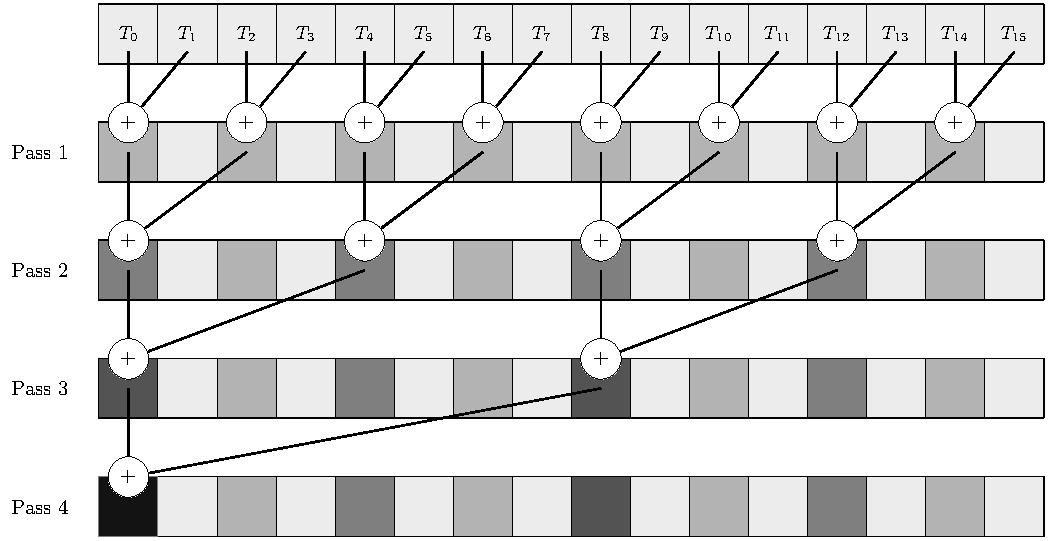
\includegraphics[width=0.75\textwidth]{./ch3_numerics/CUDA/prefixsum.pdf}
    \caption{A simplified parallel summation algorithm. After each pass the number of elements to sum is halved, leading to a $\mathcal{O}(\log{} n)$ complexity in time. Since we require only the total sum, this algorithm choses to read the value at $T_0$ at the end of the run.}
    \label{fig:prefixsum}
\end{figure}

Another typical algorithm following this is the Hadamard product (element-wise multiplication) of two vectors or matrices. Although in parallel the number of operations and complexity remains the same, the advantage comes from the lack of interdependence between elements. The multiplications can be carried out asynchronously, allowing all freely available cores to work continuously until every element pair is multiplied.


Mapping the above problems onto GPU devices requires an understanding of some of the architecture and hierarchies of the programming model. I will next introduce this model, and discuss some optimal uses of the available memory and structures.


\section{CUDA programming model}\label{sec:cuda_prog}
Although many models exist for multicore programming, for both CPU and GPU with OpenCL and OpenACC being two such examples, I will concentrate on Nvidia's CUDA \cite{NUM:Nickolls_cuda_2008}. CUDA is a mature programming model and API for Nvidia GPUs, and has been well-received for high-performance parallel computing. CUDA operates on a single instruction multiple thread (SIMT) architecture, wherein a single operation is mapped to multiple compute threads independently operating on individual units of data. Writing a program using CUDA C/C++ is very similar to standard C/C++ programming, albeit with some minor differences to account for control of GPU compute threads. CUDA manages calculations in a hierarchical structure with differing levels of fine-grained control over these threads. At the finest grained level ($T$) we have compute threads which operate directly on a single datum from memory. The maximum number of threads which can run simultaneously on the device in a single compute unit are known as a \textit{warp}. Threads are grouped into blocks ($\mathbf{B}$), which is the next hierarchical level, which will optimally contain multiples of the maximum warp number for the device (32 elements is the standard warp size for Nvidia architecture).

At the coarsest level, the blocks are grouped together into a grid ($\mathbf{G}$), which encompasses the entire problem space. Hardware limits are specified limiting the upper-values of how many elements can appear in these units, and thus the hierarchy exists to allow for fine-grained control on memory usage, and hence performance optimisation on calculations. For a given problem it is necessary to find a mapping from data values in memory to execution threads. To ensure optimal use of GPU cores, the number of threads worked on simultaneously can be (for current hardware) up to 1024 threads per block, though keeping this value divisible by the warp size is recommended to allow exact mapping to device cores. Optimal values can be found for balancing data computation and transfers, giving, depending on system size, necessary values for block size, as well as grid size. The dimensions of each hierarchical layer are independent of one another, and may be up to 3, with a hardware dependent limit only imposed on the maximum number of elements. Figure~\ref{fig:gpu_threads} gives a sample layout for a system of 2D threads, 2D blocks, and a single grid.

\begin{figure}[tb]
    \centering
    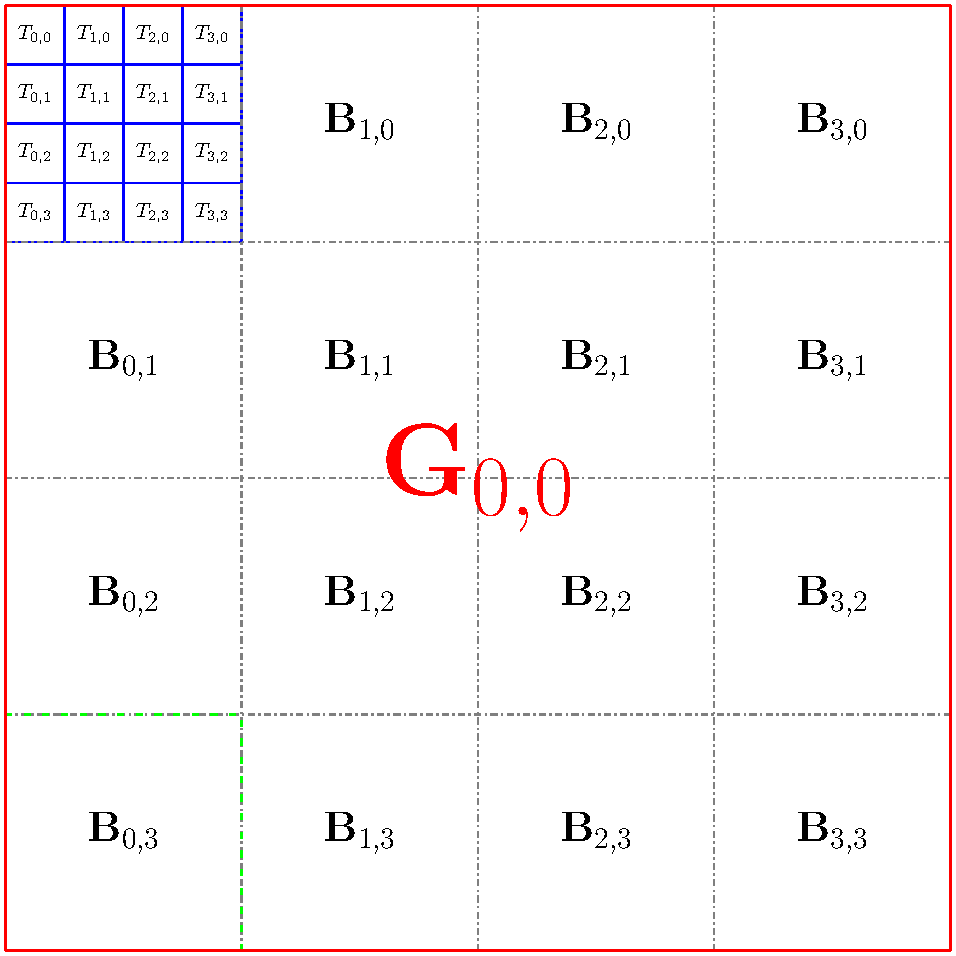
\includegraphics[width=0.6\textwidth]{./ch3_numerics/CUDA/gputhreads.pdf}
    \caption{A sample CUDA data hierarchy model. Each thread ($T_{x,y}$) has use of private memory, which offers the highest performance overall, though does not allow transfer to other threads. Data within a block ($\mathbf{B_{x,y}}$)can be treated as adjacent and accessible to all other elements in the block using {shared memory}, and is next highest in terms of performance. Transfers between blocks require the use of {global memory}, which is slowest overall. Internally all data is stored and indexed lexicographically within the grid ($\mathbf{G}_{x,y}$).}
    \label{fig:gpu_threads}
\end{figure}

It is necessary to be aware of the different aspects of managing the GPU memory. Unlike programming for a CPU-based system, GPUs require explicit control of several different types of memory. Nvidia's CUDA programming model defines these different physical memories into \textit{global}, \textit{constant}, \textit{shared} and \textit{private}. Global memory is analogous to random access memory (RAM) on a CPU-based system, and is the location where we primarily store data for computation on the GPU. This memory block is accessible (readable and writeable) to all threads in the computation. This is also the slowest memory on the GPU, with bandwidths of approximately $10^{11}$ bytes per second. Constantly reading and writing to global memory can hinder the performance of a computation. For memory that is statically defined at the start of a program and will only be read thereafter, the constant memory can be used. This is a special area of memory that can be used to store constants and other values that are often read during a computation. Once set, these values cannot be modified. The next memory level is shared memory, which is block accessible only i.e. threads within the same block have access. This allows threads to exchange information with close neighbours, and is the preferred method of inter-thread communication. Although higher performance than global, the size of shared memory is much smaller. An ideal use case is the parallel summation example given in Sec.~\ref{subsec:par_op}. Performing this algorithm requires the copying of data from global to shared memory, performing the calculations, then copying the results back. Lastly, private memory which maps directly to device cache, is thread-accessible only i.e. each thread has access only to its own private values. This memory can be used for local variables defined in a function (known as a \textit{kernel} for GPUs). Private memory has the highest performance, but the smallest available size. If possible, copying variables from global memory into private memory, performing all operations on private, then saving back to global can yield the highest performance, as global memory (slow) is read from and written to once each.

Limiting transfers between the CPU/RAM to the GPU/global memory are of high importance, as the slowest line of communication is the PCI-Express bus, connecting the GPU to the host system ($\approx 16 $ GB/s max). Eliminating unnecessary communication will almost certainly allow for a gain in performance. Mapping a problem to the GPU requires parallelising the calculation and removing transfers where applicable. For maximum performance, a sample model of performing a GPU calculation is:
\begin{enumerate}
    \item Define all variables and data on the host system.
    \item Identify the optimal mapping onto the GPU thread execution model.
    \item Send the data from RAM to the GPU global memory.
    \item Perform computation, with necessary elements copied to shared/private memory.
    \item Return final output of computation to host system when completed.
\end{enumerate}

Although idealised and highly simplified, close adherence to such a model should yield significant performance gains compared to multicore CPU-based computation. An important point with memory access in GPUs is that to ensure optimal performance all access should be assumed to be in-order and adjacent. As an example, though the parallel sum method discussed in Sec.~\ref{subsec:par_op} is superior to an iterative summation, it is not an optimal example for GPU architectures \cite{BK:Cuda_book}. With a small improvement, this can be highly optimised, as highlighted by Fig.~\ref{fig:prefixsum2}. In this case, the memory access is carried out in strided linear chunks, and by ensuring that all memory accesses are performed this way as much as possible an overall higher degree of performance can be achieved \cite{BK:Cuda_book}. As GPUs operate on blocks of memory simultaneously, minimising the amount of misaligned memory accesses can optimise the access performance. In this instance, these structures can be packed efficiently together and ensure a large number of copies are performed optimally, with coalesced memory access.

While the details are often abstracted by the internal workings of the device, an awareness of this can prove useful. If we assume the number of data elements to be summed is larger than the available number of threads, this routine can perform several passes before the threads become sub-optimally used, as in the previous case. In this way, the summation ensures that the available threads are working mostly optimally.

\begin{figure}
    \centering
    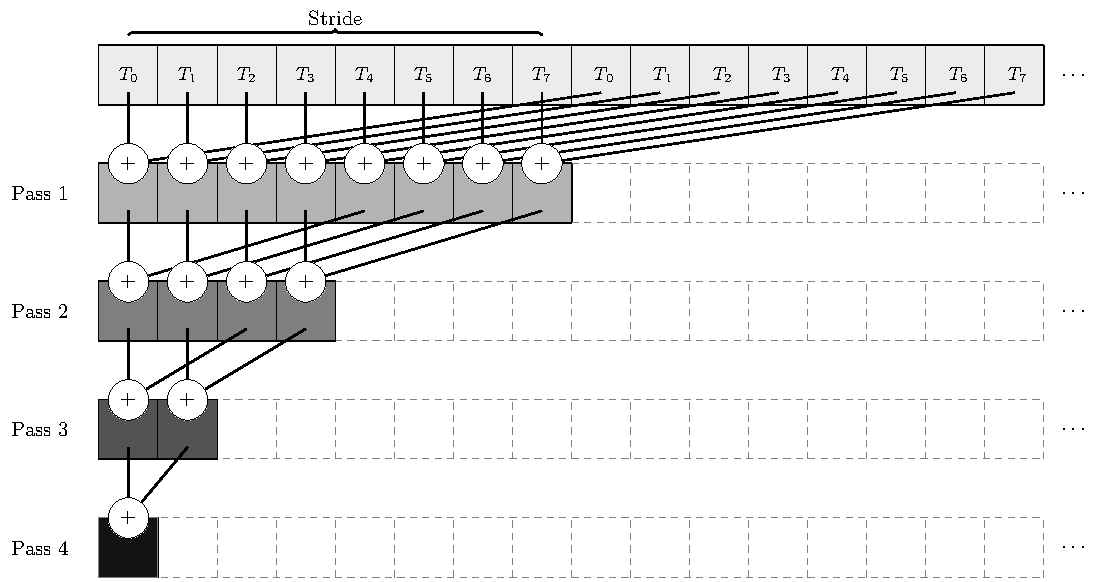
\includegraphics[width=0.75\textwidth]{./ch3_numerics/CUDA/prefixsum_2.pdf}
    \caption{An optimised parallel summation, which allows for strided memory access. By halving the size of the stride and block size at every increment the number of evaluations carried out simultaneously will better utilise the available GPU cores.}
    \label{fig:prefixsum2}
\end{figure}

Given that GPUs are first and foremost image processing devices, their ability to perform Fourier transforms rapidly is a well developed strength. Due to the large number of available cores, fast Fourier transforms (FFTs) can be significantly faster on a GPU than performing the same operation on many CPUs \cite{AO:Morgan_pra_2013}. The CUFFT library allows for a seamless way to take advantage of this performance increase using GPUs. Next, I will discuss an example of GPU-enabled simulations for an experimentally realistic problem making use of the GPU to perform the necessary operations discussed in Sec.~\ref{sec:timeev},\ref{sec:fso}, and offer some realistic performance measurements.

%\section{3D STIRAP using GPU}
%For performance metrics, I will discuss the use of a GPU-enabled Schr\"odinger equation integrator developed by myself, comparing the results to a multi-core MPI enabled version by T. Morgan and N. Crowley. We solved the Schr\"odinger equation for a fully three-dimensional potential, demonstrating its accuracy and improved performance compared to standard HPC methods.

        \section{GPU-enabled parallel Schr\"odinger simulations}
\label{sec:3D Stirap parallel Schr\"odinger simulations}
For performance metrics, I will discuss the use of a GPU-enabled Schr\"odinger equation integrator developed by myself, based on and compared with the results to a multi-core MPI enabled version by T. Morgan and N. Crowley. We solved the Schr\"odinger equation for a fully three-dimensional potential, demonstrating its effectiveness and improved performance compared to standard HPC methods.

The problem we examined was that of a realistic system for coherent atomic control. Controlling the centre-of-mass movement of atoms between adjacent trapping potentials via adiabatic techniques, collectively known as \textit{spatial adiabatic passage} (SAP), has recently become a popular topic of investigation [cite review]. The STIRAP process [cite] is a widely studied and used optical technique for controlled state transfer. Herein I describe the motivation, physical system, and the numerical implementation for solution of this problem.

\subsection{Spatial adiabatic passage}

Significant work and progress has been made for control of the internal degrees of freedom of atoms. External degrees of freedom are, however, only recently being made realisable. The use of adiabatic techniques such as the SAP family of methods are very promising tools for high fidelity state generation and transfer. One such technique from this family is known as {\textit matter-wave STIRAP}[cite], which is an analogous technique to that of STIRAP in optical systems. This technique can be used for high fidelity atomic centre-of-mass control \cite{Eckert:04}, and can be used to transfer atomic population between trapping potentials due to its highly robust to variation in the system parameters. The use of this technique has recently become experimentally accessible [private communication with S.~Taei from group of Y.~Takahashi], although many other accessible systems have been proposed \cite{Eckert:06,Morgan:11,Kohler:13,Morgan:13}.

If we initially consider two separated harmonic potentials (traps), with groundstates given by $| L \rangle$ and $| R \rangle$, a reduction of the distance between the traps will increase the coupling, and hence tunneling rate, between them. This is modeled with the two-level Hamiltonian as
\begin{equation}
    H = -\hbar
    \begin{pmatrix}
        0 & \Omega_{LR} \\
        \Omega_{RL} & \Delta
    \end{pmatrix}
\end{equation}
where $\Omega_{LR} = \Omega_{RL}$ are the couplings between states, and $\Delta$ is the detuning of state $| R \rangle$, relative to $| L \rangle$. Assuming an atom initially localised in $| L \rangle$, and with an increase in coupling strength between the levels, the localised atom will tunnel from $| L \rangle$ to $| R \rangle $. However, this processes is difficult to control, as Rabi oscillations introduce an explicit time-dependence and cause the atomic population to continuously transfer between both traps. This will require precise timing and control to ensure a fully robust transfer of population. Thus, a double-well potential is a difficult system in which to realise coherent control.

A more robust method, using three adjacent harmonic traps and the aforementioned matter-wave STIRAP process, improves upon the double-well system. For this SAP technique, we model the adjacent trapping potentials as coupled by their nearest neighbour solely. For three such potentials, $L,M,R$, on resonance,  this is given by the Hamiltonian
\begin{equation}\label{eqn:sap_ham}
    H = -\frac{\hbar}{2}
    \begin{pmatrix}
        0 & \Omega_{LM} & 0 \\
        \Omega_{LM} & 0 & \Omega_{MR} \\
        0 & \Omega_{MR} & 0
    \end{pmatrix},
\end{equation}
where $\Omega_{LM},~\Omega_{MR}$ describe the coupling between left-middle and middle-right potentials respectively. Diagonalising this Hamiltonian gives three distinctive eigenstates, however only one is of interest here. For the $\lambda=0$ eigenstate of this Hamiltonian, known as the \textit{dark state}, the dependence on the middle potential vanishes, with the state given by
\begin{equation}
 | 0 \rangle = \cos\ \Theta| L \rangle - \sin \Theta | R \rangle
\end{equation}
where $\Theta=J_{MR}/J_{LM}$ is the mixing angle. From the adiabatic theorem of quantum mechanics, it is known that if an eigenstate has its Hamiltonian perturbed slowly enough, then we can follow its evolution ensuring that it always remains in an eigenstate of the Hamiltonian. Thus, by preparing the system in state $| L \rangle$, and varying $\Theta$ slowly, we can shift the population from the leftmost harmonic potential to the rightmost, without populating the center.

\begin{figure}
    \centering
    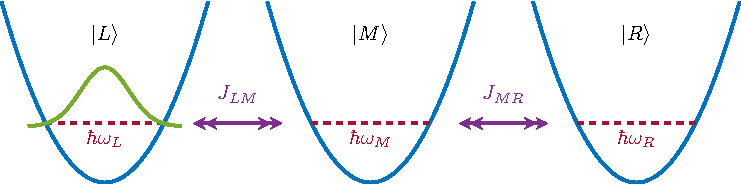
\includegraphics[width=0.75\textwidth]{./ch3_numerics/3potentials}
    \caption{Three trapping potential model for matter-wave STIRAP. The atom (green) is initially localised in the leftmost potential, $|L\rangle$, with the couplings between adjacent traps controlled by varying the distance dependent parameters $J_{LM},J_{MR}$.}
    \label{fig:ch3_stirap}
\end{figure}

This technique makes use of tunneling, with the rate of transfer between trapping potentials controlled by the respective spatial separation, and is demonstrated by Fig.~\ref{fig:ch3_stirap}. Typically, the method would be performed with time-dependent potentials. However, a static potential variant can be considered using parallel atomic waveguides, wherein the separation varies as a function of distance along the parallel axis. If we consider an atom that travels along such a waveguide, the coupling and hence tunneling rates seen by the atom in the waveguide are altered as the atom propagates. Such work has been discussed and considered in a realistic system for two spatial dimensions \cite{OSullivan:10}. Although a two dimensional model will be effective at describing much of the relevant dynamics, the lack of $z$-dimension ensures the effects stemming from dispersion, curvature of the waveguides and the absence of any such eigenstates along $z$ reduce the realism of such a model.



Thus, the goal of this project was to develop a realistic system for controlled movement of atoms with high fidelity amongst trapping potentials. The atomic population transfer between traps is controlled by the tunneling rate, through variation of the spatial separation between adjacent traps. It is instructive to note the counter-intuitive change of couplings between these potentials. For an atom initially located in the left potential, we increase $J_{MR}$ for the empty middle and right traps, before reducing again and increasing $J_{LM}$ for the left and middle. This is in direct contrast with a direct tunneling scheme, for which we directly increase the coupling between the populated left and empty middle, followed by middle and right. However, the direct scheme can be seen as two distinct combinations of the double-well case, and so carries the same time-dependent Rabi-oscillations. Comparing both methods will be instructive in discussing the advantages of the SAP routine over direct tunneling. %I will first discuss the physical model of this system.


\subsection{Physical model}

As discussed previously, to fully understand the dynamics of such a system we must investigate the fully three-dimensional model. One method of creating the required potential landscape is through the use of atom chips \cite{Bartenstein_ieee_2000}[cite Atoms and Wires: Toward Atom Chips]. These systems consist of micro-fabricated current-carrying wires, and can be used to create a variety of trapping potential shapes. With the application of current a magnetic field is created around individual wires, of which has a minima at the wire core. By applying an additional field orthogonal to the direction of current, this minima can be raised to a location above the wire surface, and can behave as a trapping potential for atoms, with an additional field applied to prevent Majorana losses in the trap. Spatial and temporal adjustments of the potentials are possible, with a fine degree of control. These have been used extensively in recent years for trapping potentials [cite], and as atomic manipulators [cite].

For this work, the system was modeled as three adjacent wires on the atom-chip surface. By applying current and the appropriate magnetic fields to these wires, magnetic minima would be created to act as atomic waveguides. To avoid dispersion, and ensure the atom moved along the waveguide, a harmonic oscillator potential was also added along the parallel axis. The process of simulating the system involved localising the atom by a barrier at one end of the $|L\rangle$ potential, with the system evolved in imaginary time to find the groundstate. After finding the the groundstate, the barrier was removed, and the atom was allowed to propagate along the length of the waveguide. The populations in each waveguide could be tracked and calculated at each step of the process, with the final populations taken as the atom approached the end of the harmonic oscillator. The fidelity of the process could then be calculated by comparing the initial $| L \rangle$ and final $|R \rangle$ populations, as well as any intermediary $| M \rangle$ populations. Thus, to fully examine all such dynamics of the system, it is essential to investigate a fully three-dimensional model, which can take into account non-idealised real-world parameters.

Given that fully three-dimensional simulations of the Schr\"odinger equation are numerically expensive, the use of GPU computing methods are an ideal candidate for accelerating the simulation \cite{Bauke:11}. I will now discuss the resulting data and metadata of the simulations.



%%


\subsection{GPU computing performance}

%As fully three-dimensional simulations of the Schrodinger equation are challenging numerically, the use of GPU computing is an effective way to overcome many of the barriers. Whereas traditional computers perform computations using the central processing unit (CPU), GPU computing allows some of the work to be offloaded to the graphics processor.
As discussed in Section \ref{gpu section}, one example where GPGPU computing offer large performance gains are fast Fourier transformations (FFTs), with the Fourier split operator method being an ideal candidate for GPU systems \cite{Bauke:11}. The body of work for implementing this algorithm was using C, CUDA and Nvidia's CUFFT libraries for the Fourier transforms, whereas the MPI-enabled code similarly, was implemented using C.

To demonstrate the performance offered by GPU computing we compared it to using FFTW with MPI, a well used parallel programming paradigm and library. The message passing interface (MPI) implementation allows the code to be run across multiple machines, benefiting from the parallelism which may be offered by a supercomputing cluster. Although MPI-enabled FFTW is fast and supports extremely large grid sizes, it requires cluster access of a significant size to be a viable option. The MPI work on this project was carried out on the ICHEC system Stoney over the period 2011 to 2012, with all performance metrics data calculated therefrom.



Due to the hardware limited memory on the GPU, and that the dynamics along the $x-z$ plane were of most importance, the grid-size of the simulations were scaled as $256\times 64\times1024$ ($x\times y\times z$). Of next importance was the timestep of the simulation.  To ensure minimal loss in precision, the timestep of the simulations were chosen as $\Delta t = 1\times 10^{-6}$ s. For the GPU simulations, the test system was an Intel Core i7 2600K CPU at stock frequency, 8GB DDR3 memory operating at 1600 MHz, 7200 RPM HDD, Nvidia GeForce GTX 580 with 3GB of onboard memory running at 783 MHz GPU core frequency, 1566 MHz shader processor frequency, and 2010 MHz memory frequency. For all simulations the desktop was running Ubuntu 11.10 64-bit operating system and all calculations were performed in double precision (64-bit floating point) where applicable.

Table \ref{tbl:timing} shows the approximate timings for the completion of runs on GPU and CPU. Not only does GPU computing offer a 6-fold improvement over a single CPU, it also allows us to achieve a performance level which is comparable to an 8-node 8-core (64 cores) core MPI enabled CPU calculation. For a modest choice of GPU this offers substantial performance gains.

\begin{table}[tb]
  \begin{center}
    \begin{tabular}{|c||c|c|c|}
      \hline
      Device & Num. Devices & Timing  & Rel. Improvement \\ \hline
      CPU (MPI) & 8 & $\sim$6 Hr & 1.0$\times$ \\
      & 16 & $\sim$4 Hr & 1.5$\times$ \\
      & 32 & $\sim$1.5 Hr & 4.0$\times$ \\
      & 64 & $\sim$1 Hr & 6.0$\times$ \\ \hline
      GPU & 1 & $\sim$1 Hr & 6.0$\times$ \\ \hline
    \end{tabular}
  \end{center}
   \caption{The approximate times taken to simulate the propagation of an atom through our atom chip system on both GPU and CPU.}
   \label{tbl:timing}
\end{table}



\subsection{3D Simulations}
\label{sec:Results}

Given the large parameter space over which this system could be optimised, many simulations were required to determine optimal system behaviour. Making use of eight Nvidia M2090 GPUs available at OIST, terabytes of numerical results were generated in a relatively short time. The simulations assumed a single $^{6}$Li atom localised in the left waveguide. Its transversal wavefunction was determined numerically, with the assumption of a longitudinal Gaussian profile of similar width. The atom was then allowed to propagate along the waveguide potential, with the tunneling region at the centre of the chip.

The simulations allowed the verification of the addition of the magnetic fields at the center of the atomchips, which in turn drives the central potential out of resonance with the outer two. By adjusting the current in the central wire, such that the magnetic minima was in resonance only within the tunneling region allowed the matter-wave STIRAP process to work as expected. The resulting potentials for equal and optimal currents are given by Fig.~\ref{fig:equaloptcurrent}, showing a slice along $x-z$ and $x-y$ planes for both cases.

The populations for both the direct tunneling case, and matter-wave STIRAP processes are shown in Fig.~\ref{mwsVsDT}, with the wavefunction probablity density in the tunneling region given in Fig.~\ref{mwsVsDT}. The direct tuneling case can be seen to show large Rabi oscillations across the potentials, with the MWS process showing a much cleaner transfer, with minimal occupation of the central potential.

\begin{figure}[tb]
    \centering
  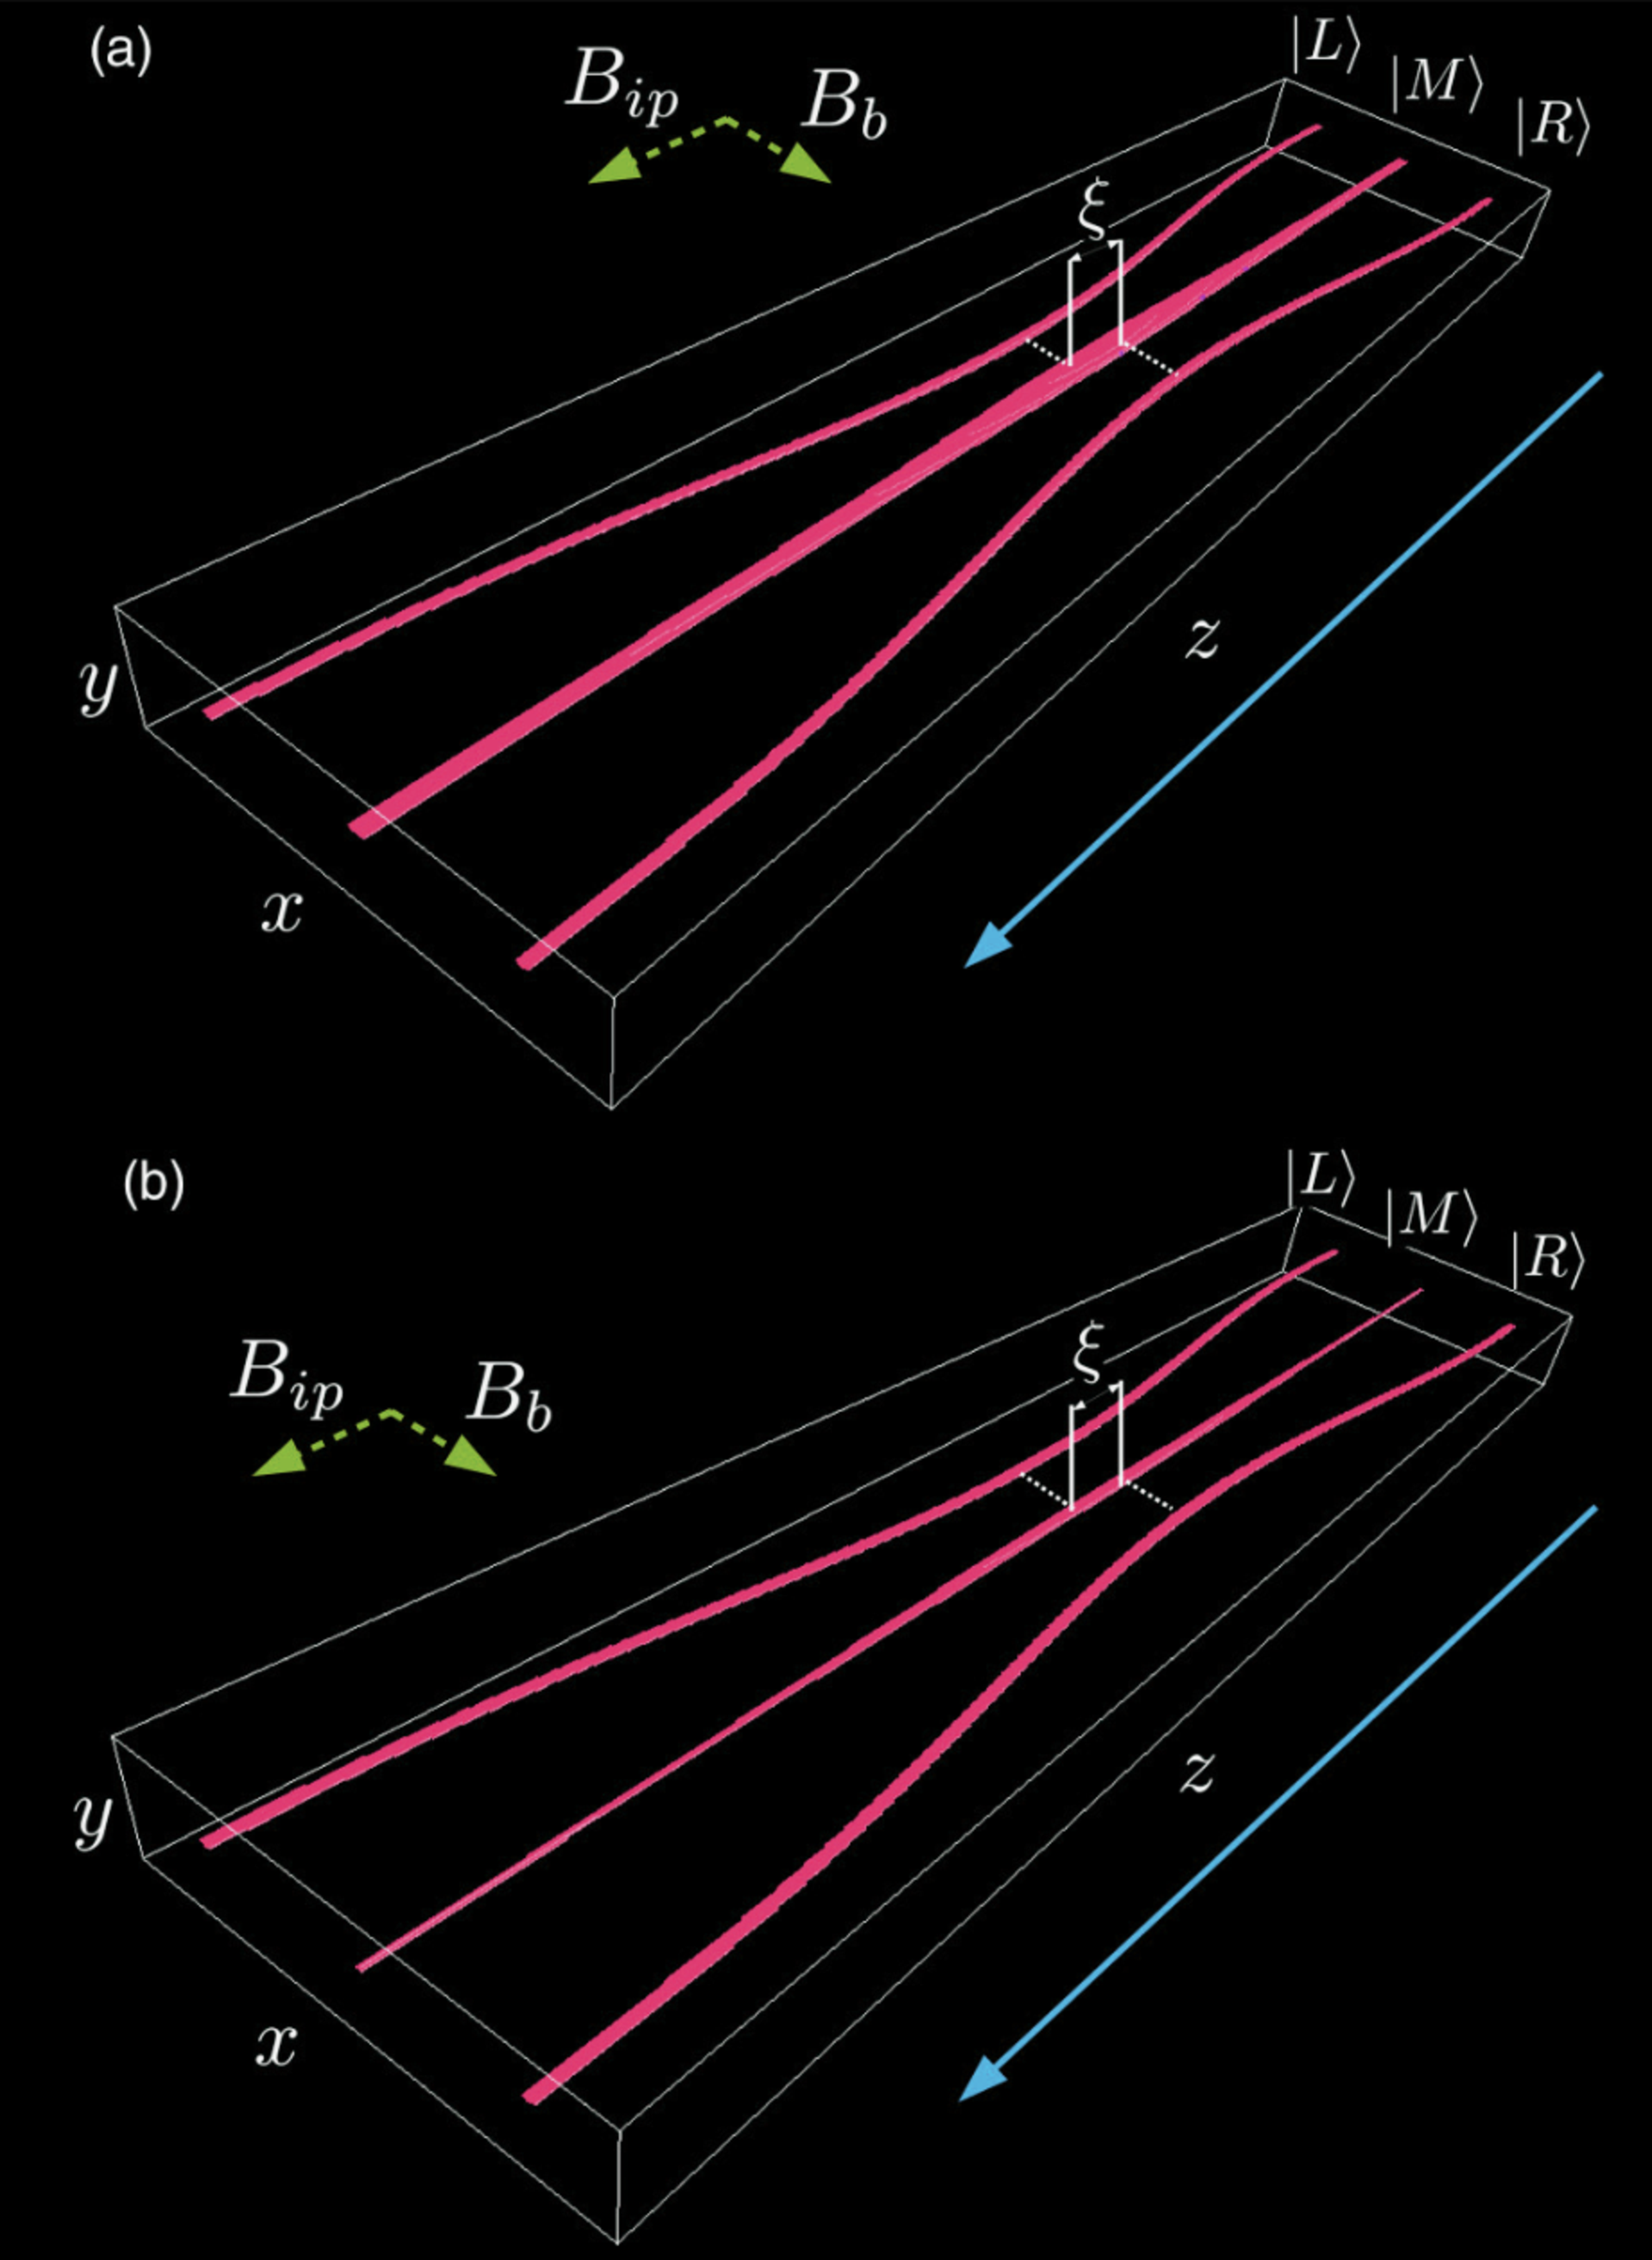
\includegraphics[width=0.85\textwidth]{ch3_numerics/3dpot.pdf}
  \caption{3d}
  \label{fig:Populations}
\end{figure}

\begin{figure}[tb]
    \centering
  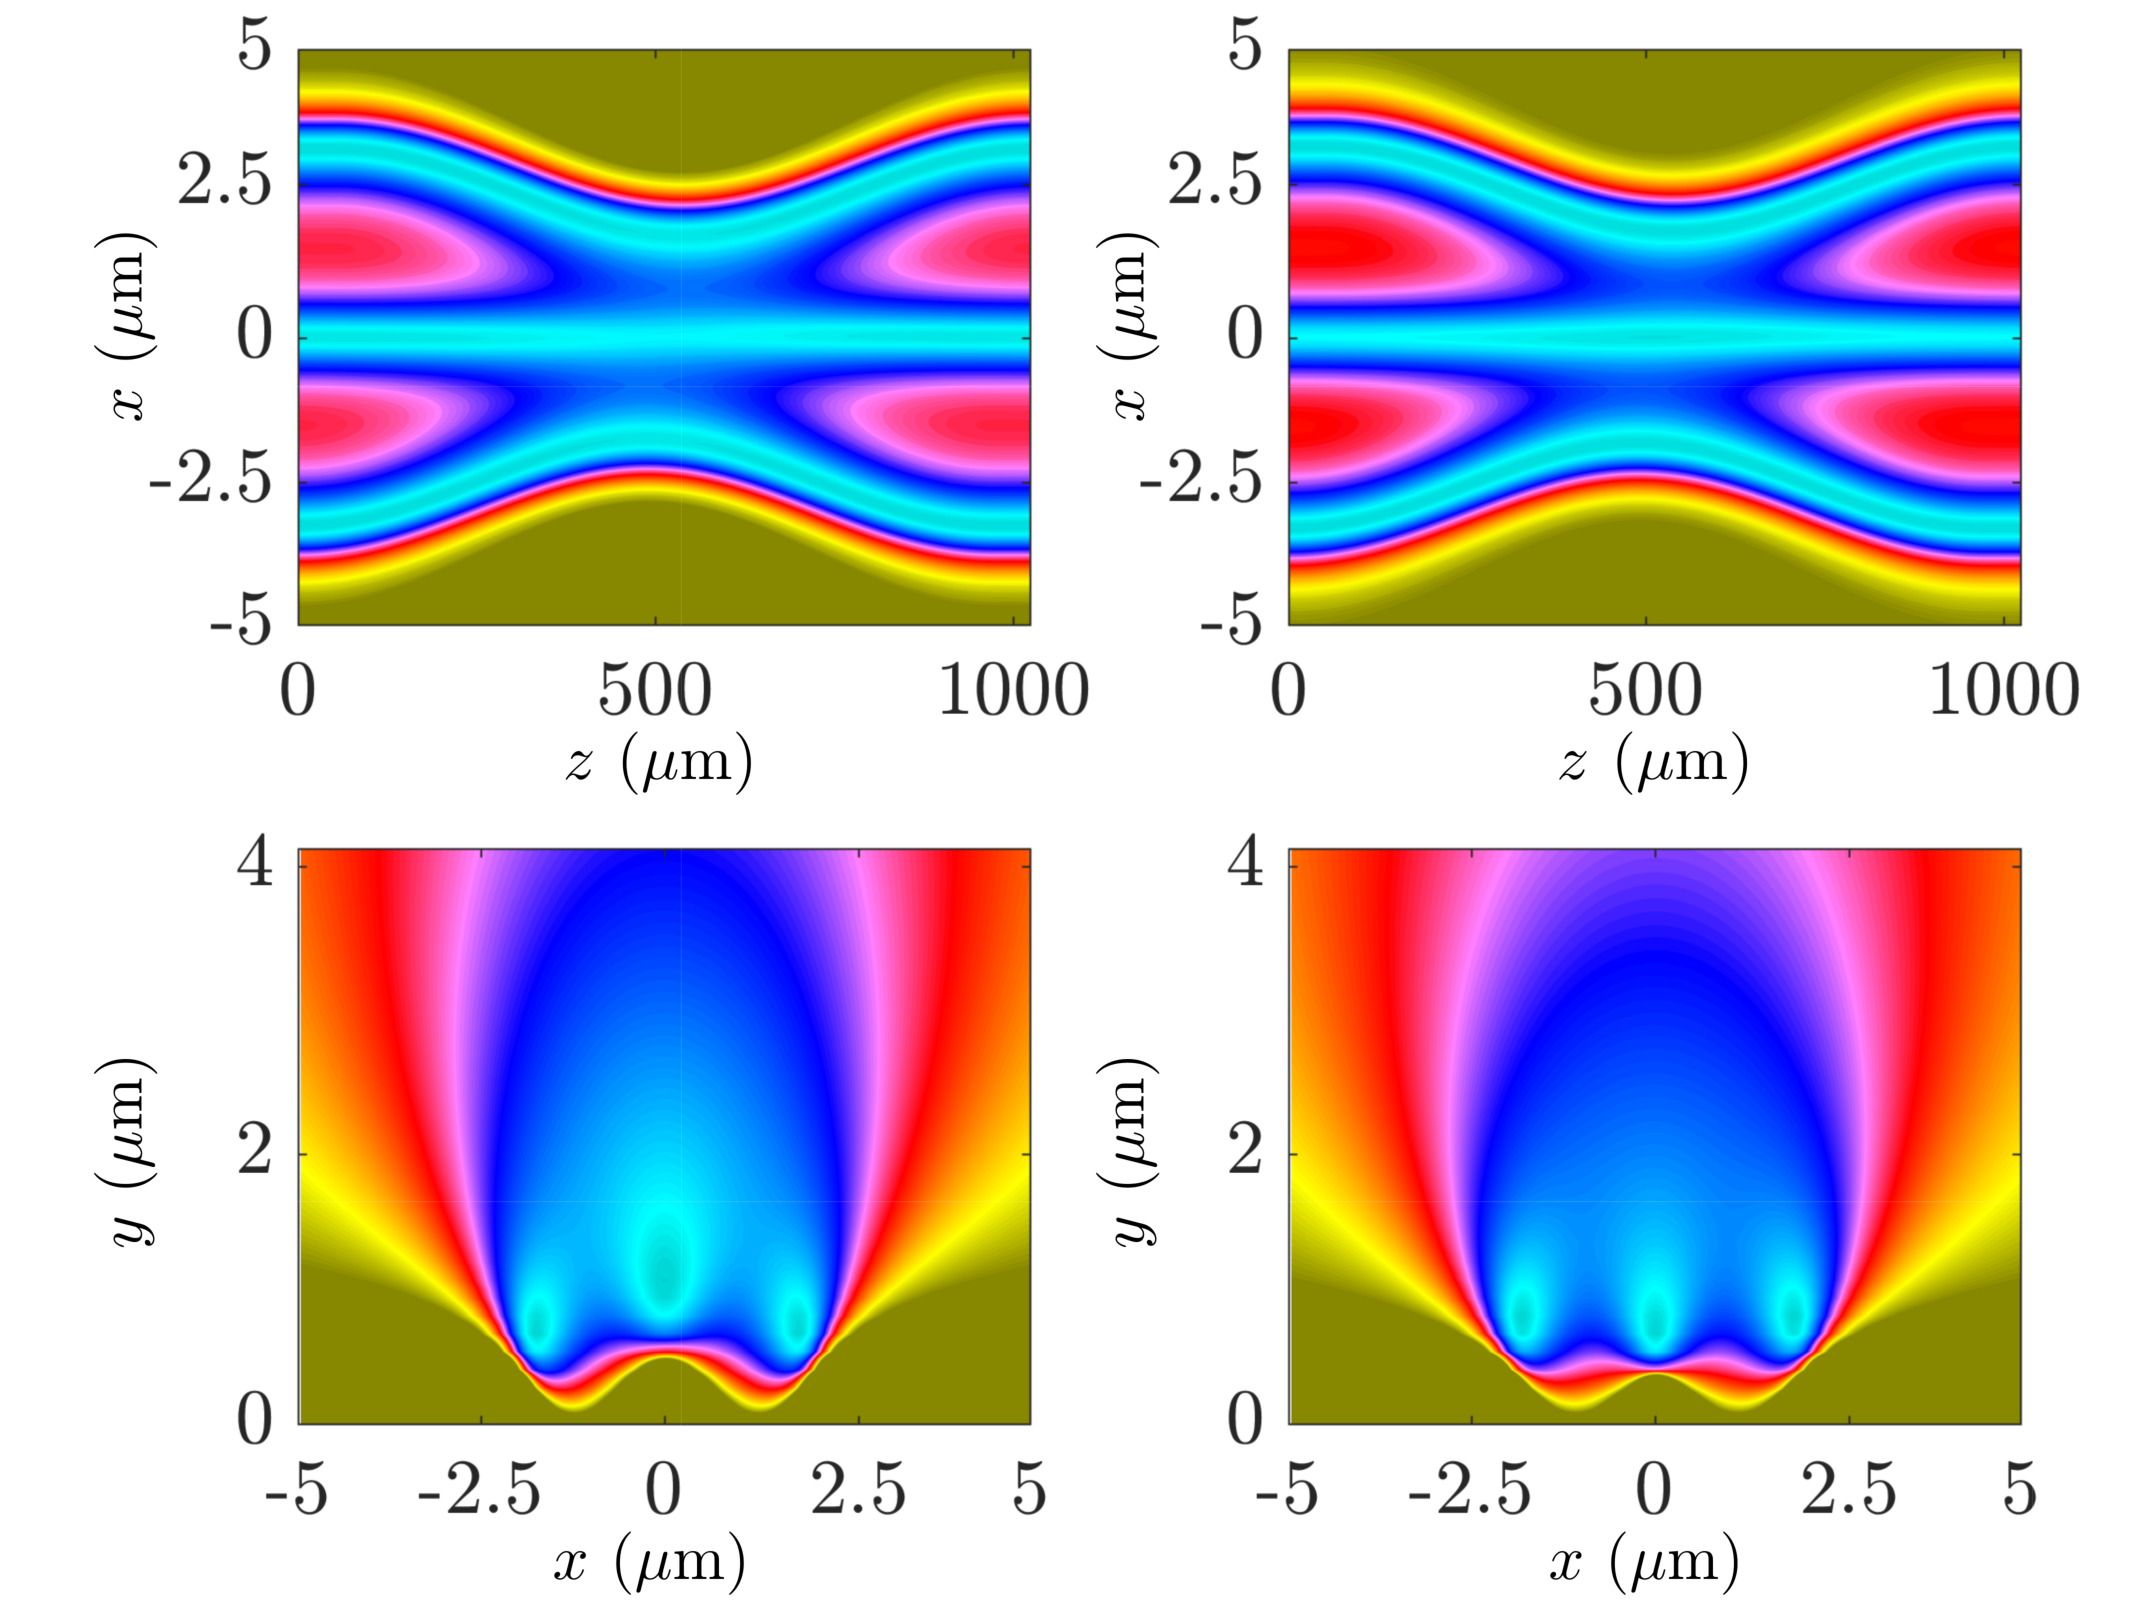
\includegraphics[width=0.85\textwidth]{ch3_numerics/potentials2.pdf}
  \caption{(Color online) The population in the left (blue dashed line), middle (green dot-dash line) and right (red solid line) waveguides as a function of time for (a) the counter-intuitive waveguide arrangement and (b) for intuitive, direct tunnelling one. The current in the middle wire is reduced to $I_M=0.07 A$.}
  \label{fig:Populations}
\end{figure}

\begin{figure}[tb]
    \centering
  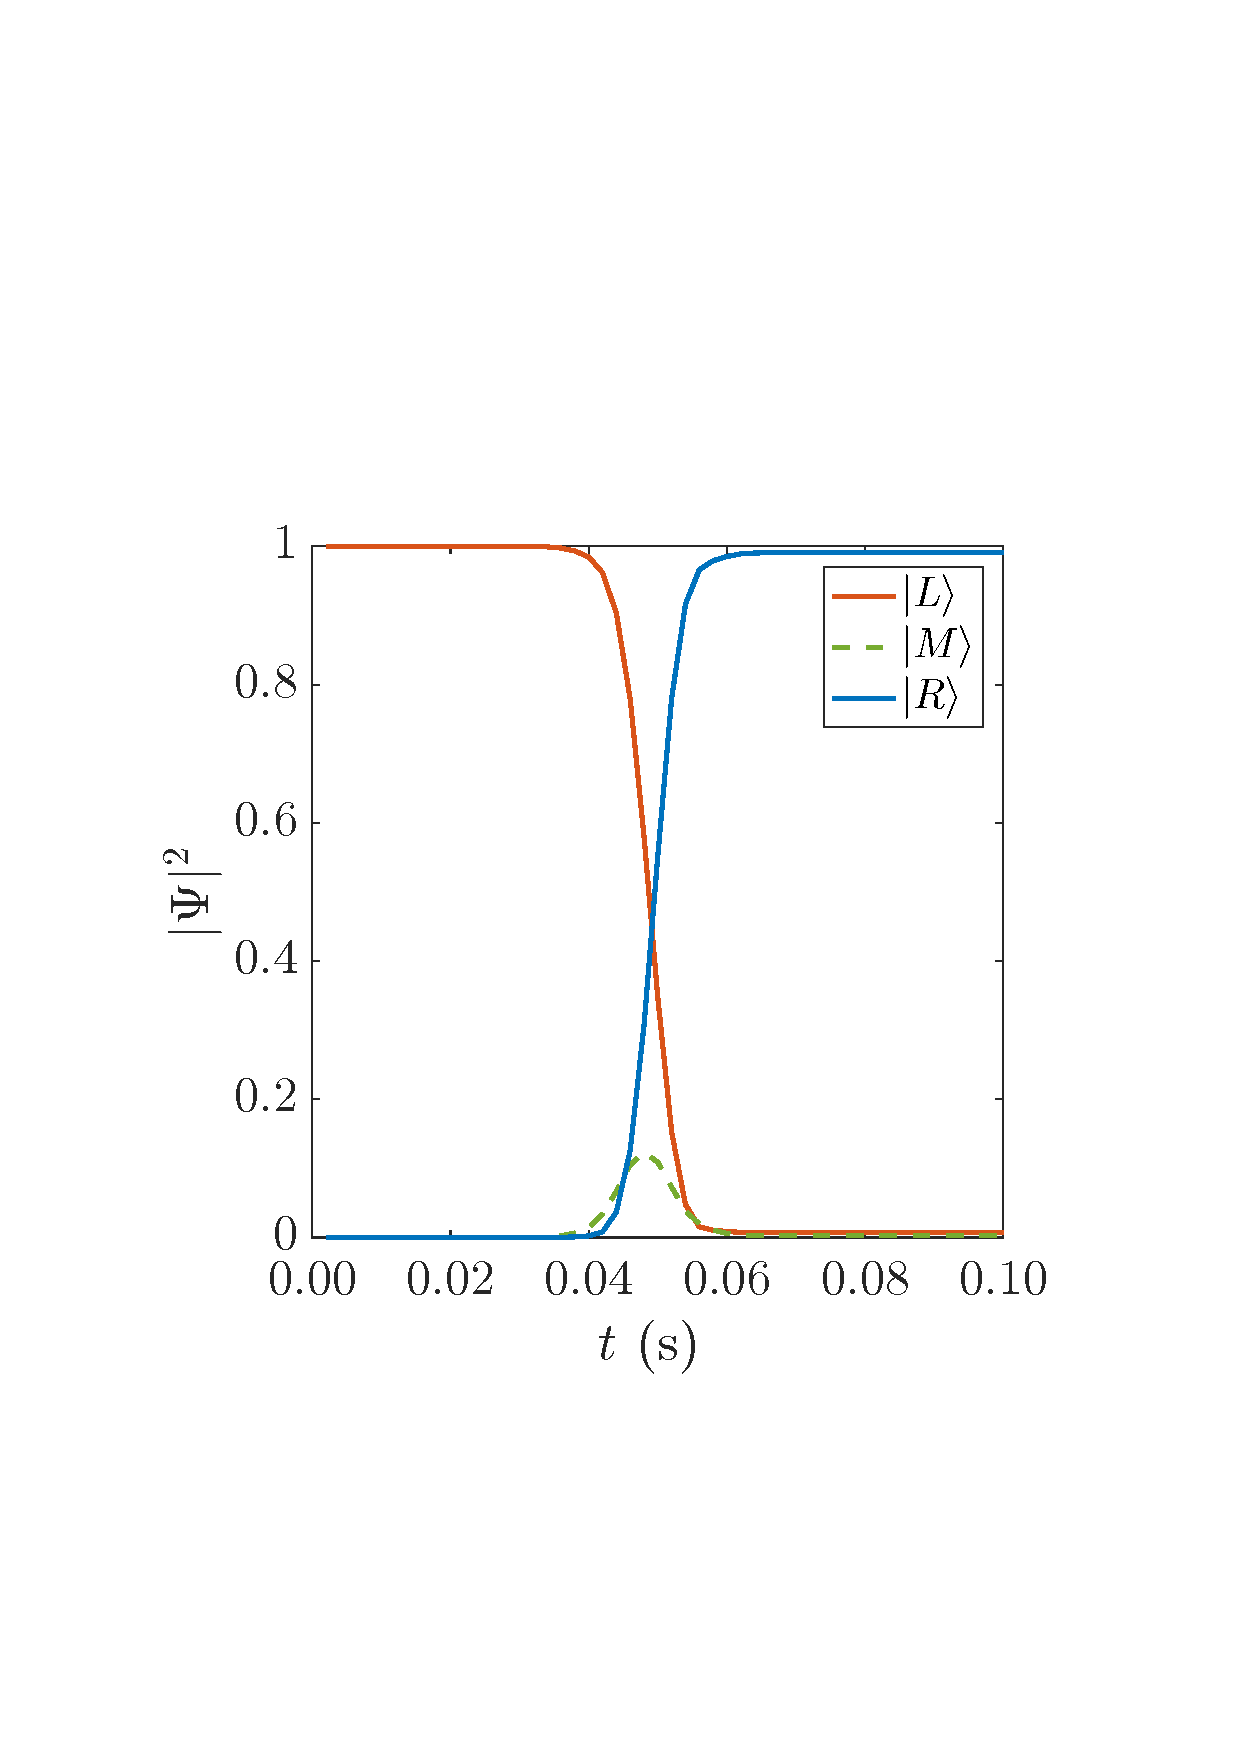
\includegraphics[width=0.47\textwidth]{ch3_numerics/STIRAP_CINT_POP}
  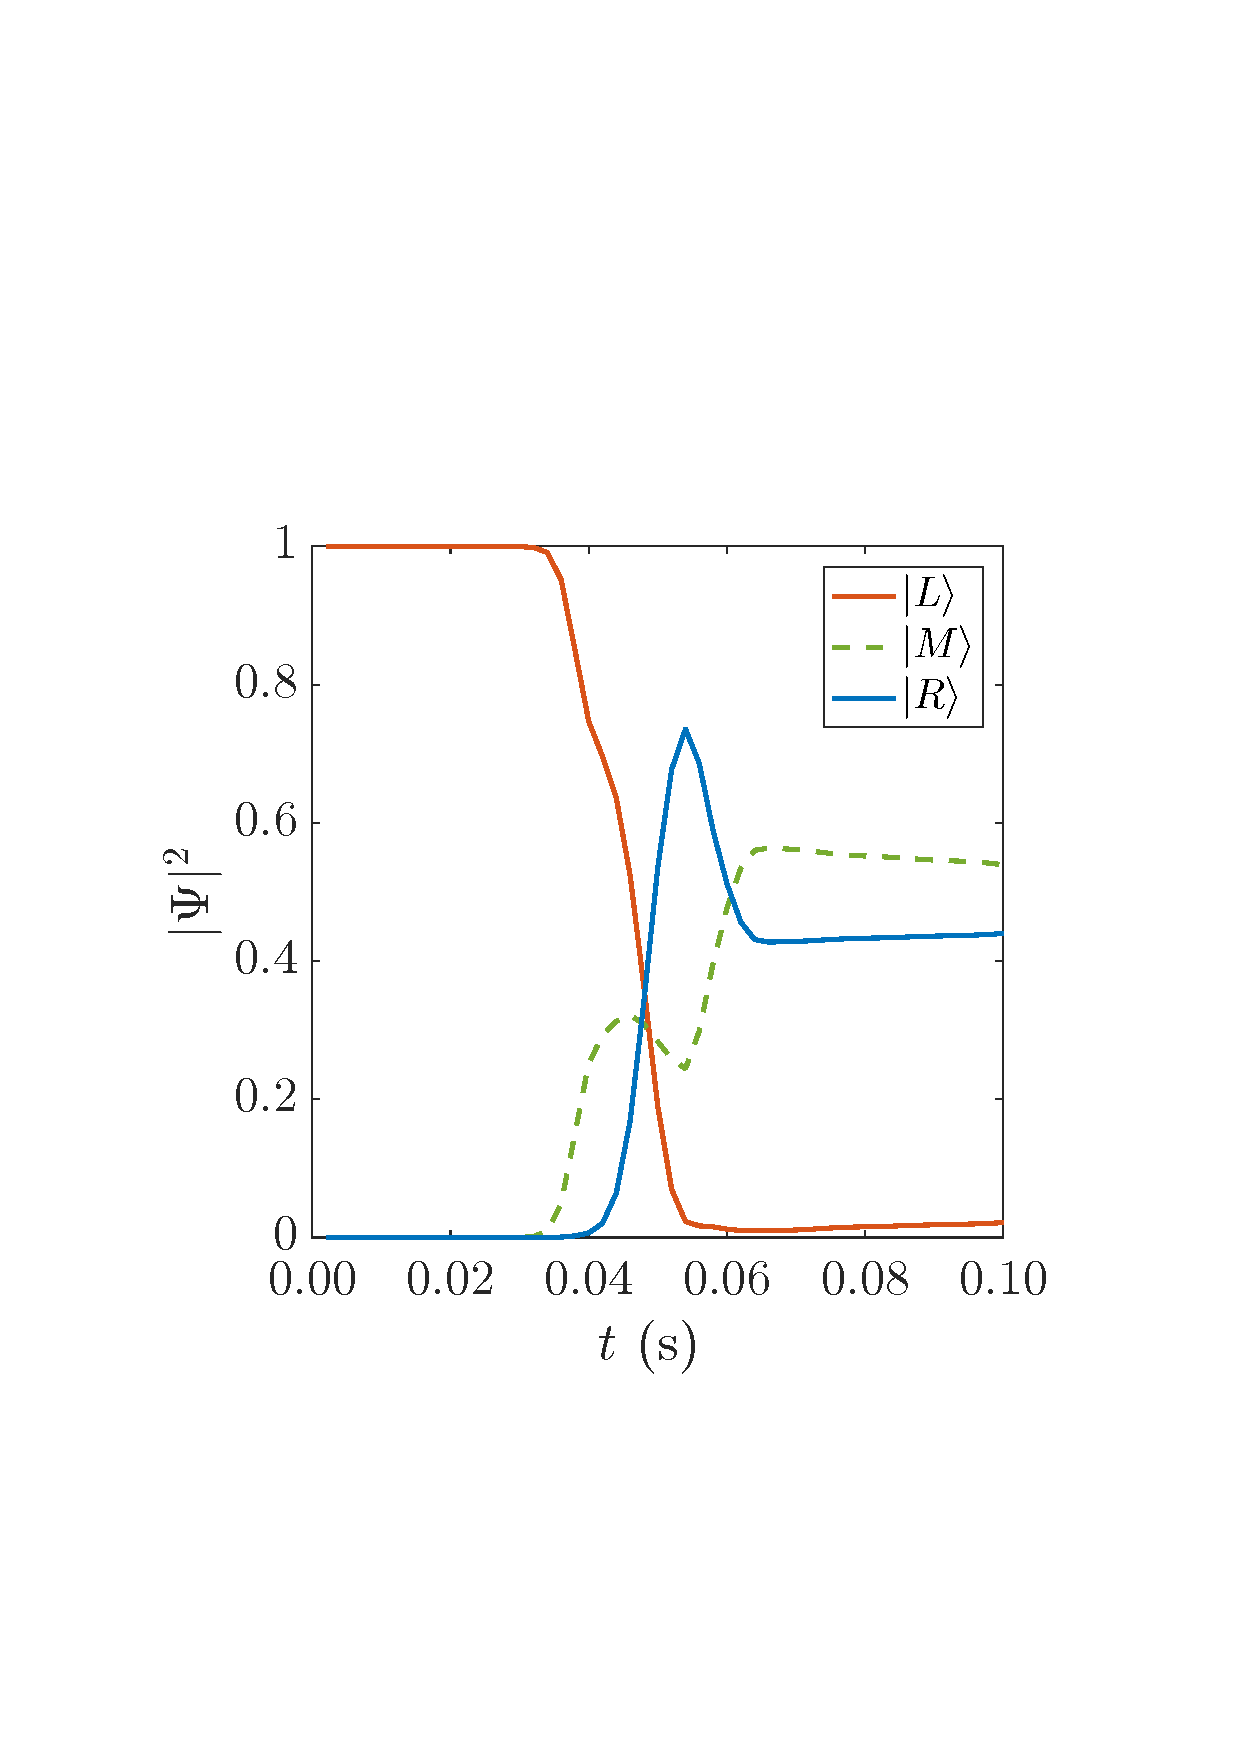
\includegraphics[width=0.47\textwidth]{ch3_numerics/STIRAP_INT_POP}
  \caption{pop}
  \label{fig:Populations}
\end{figure}

\begin{figure}[tb]
    \centering
  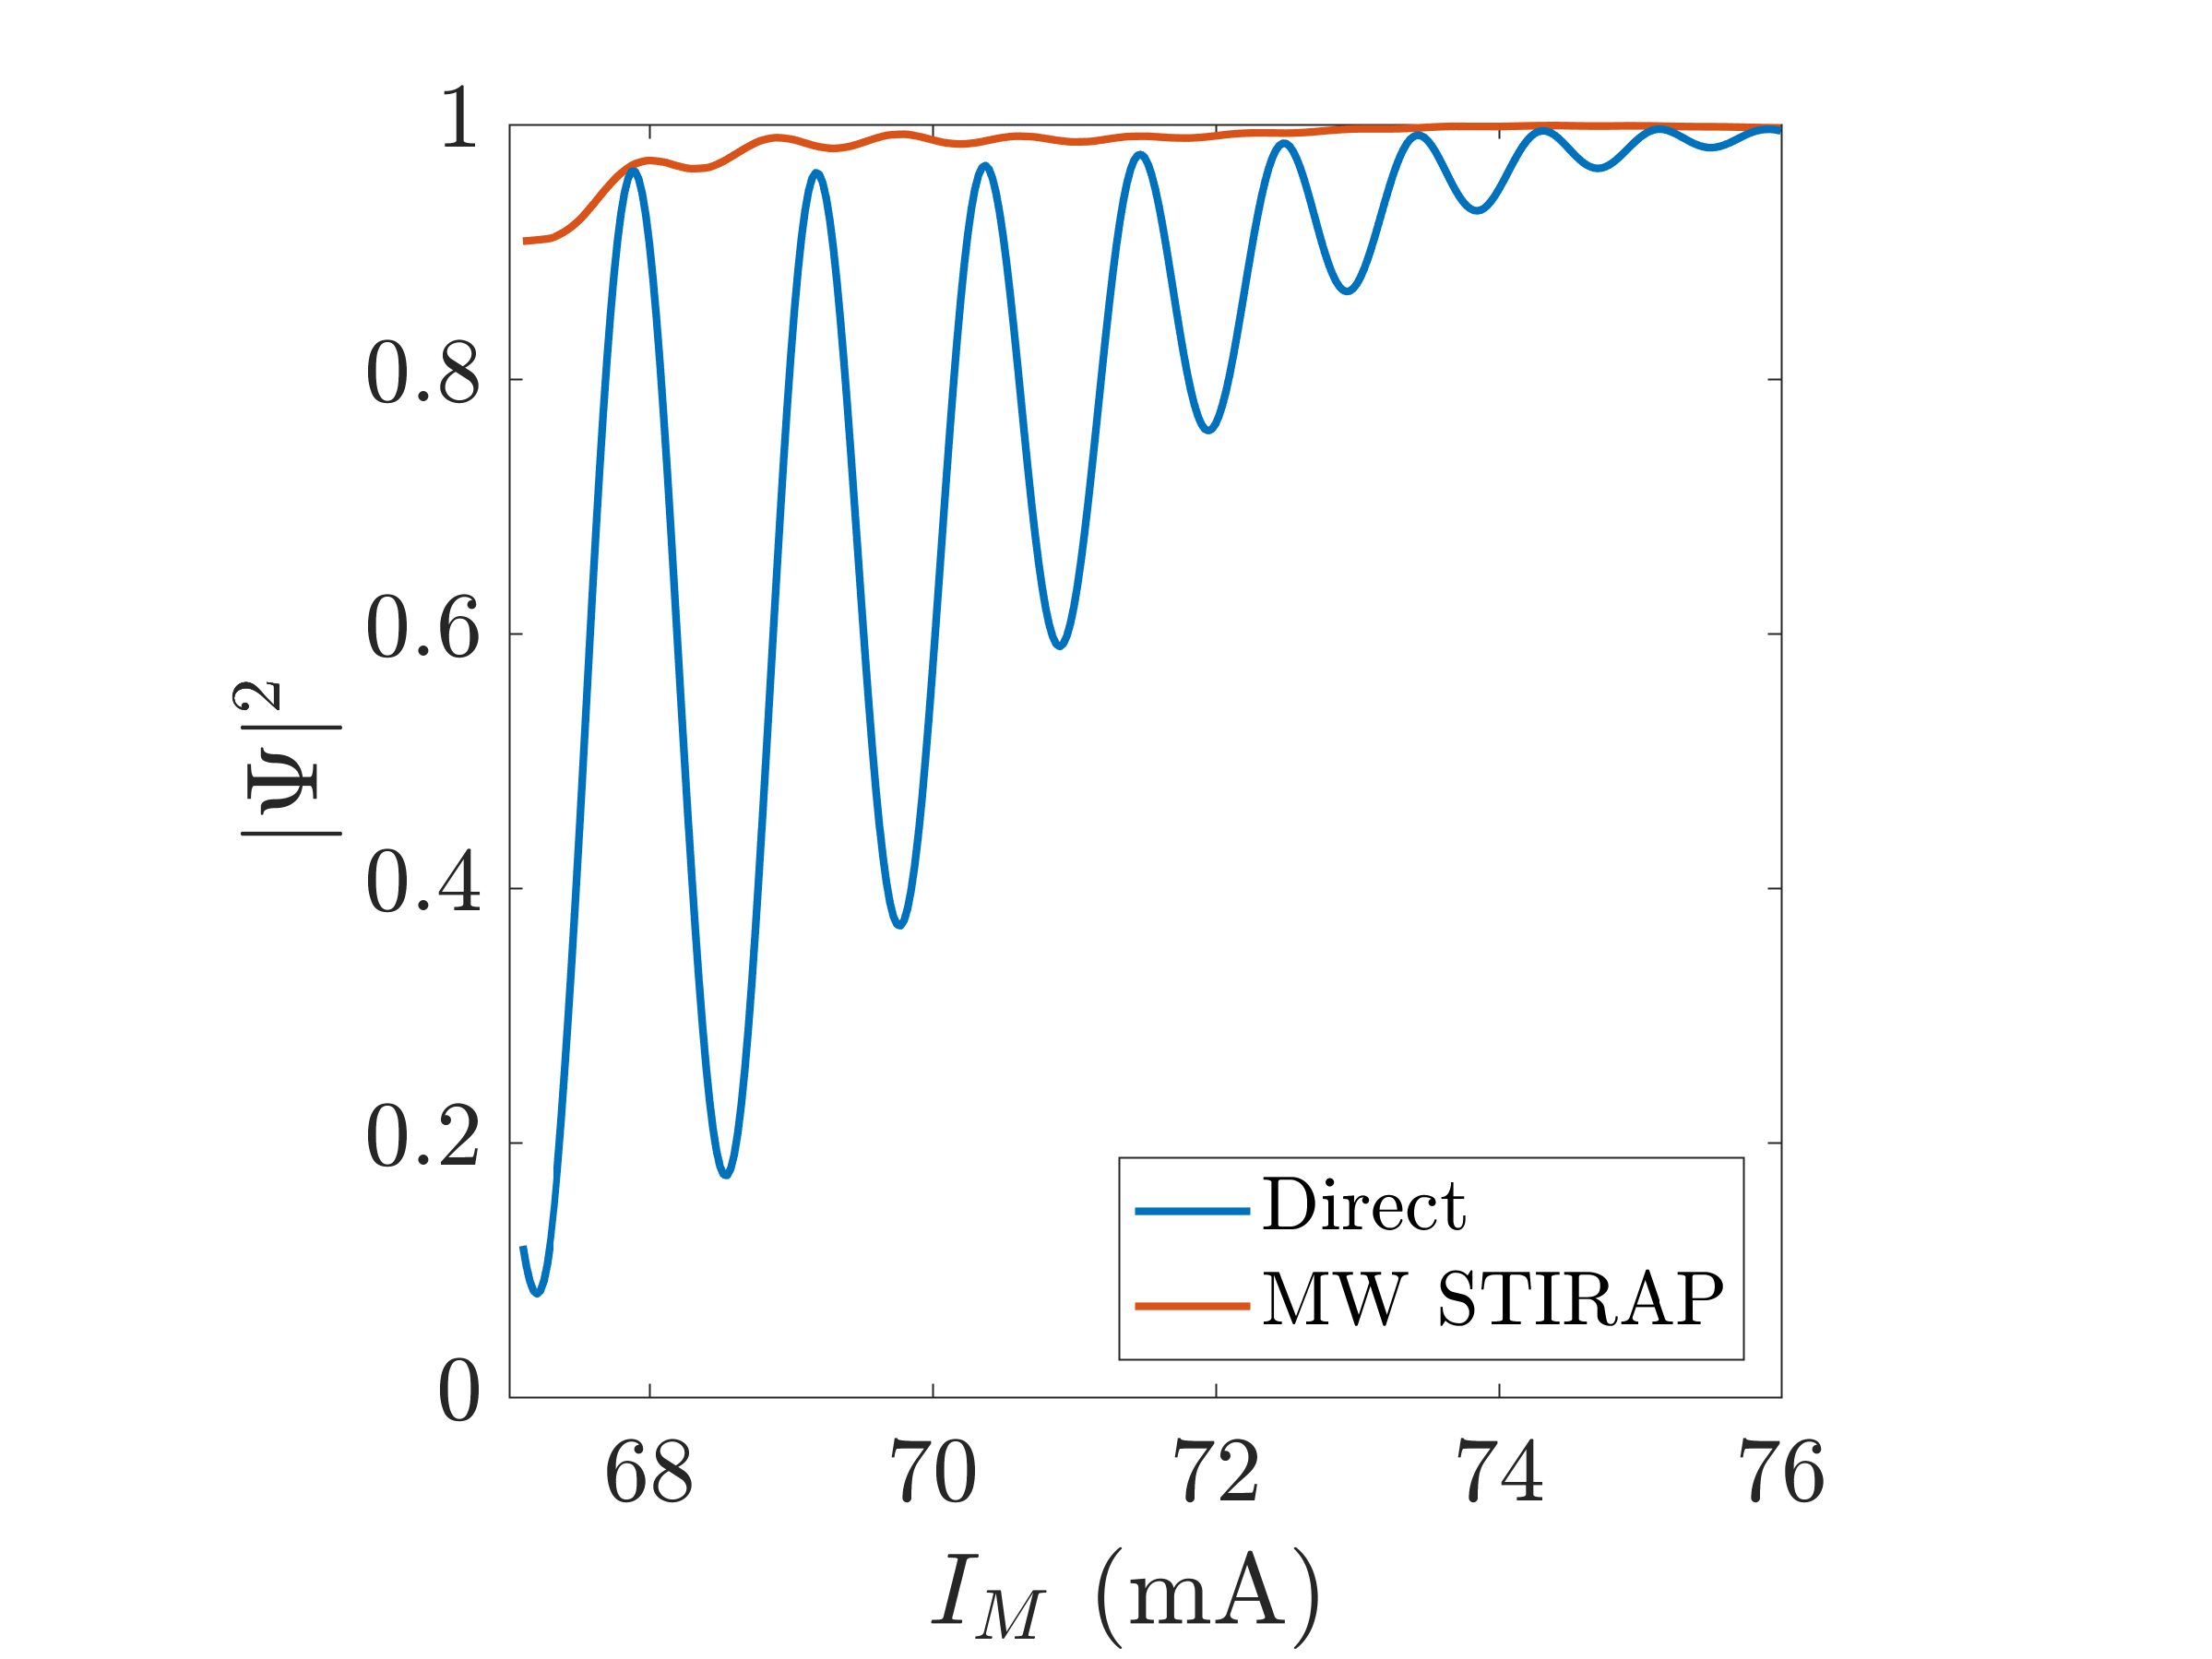
\includegraphics[width=0.85\textwidth]{ch3_numerics/DIRVSMWSTIRAP.png}
  \caption{pop}
  \label{fig:Populations}
\end{figure}

        \section{GPUE: GPU Gross--Pitaevskii equation solver}

Given the effectiveness of GPU computing in completing the simulation of a linear Sch\"odinger equation system, I next applied the newly-developed techniques to simulating Bose--Einstein condensates, which formed the bulk of work during my thesis. The body of work developed for this new project has been realeased as the software tool ``GPUE'', available at \url{https://github.com/mlxd/gpue}. Performance metrics of this code was carried out by Peter Wittek, ICFO, Barcelona [cite website]. The comparison was performed with GPUE, the Trotter-Suzuki package developed by Wittek \textit{et al}, and the mature GPELab software suite for MATLAB [url]. The sample results taken for time evolution are given by Fig.~\ref{fig:gpuevsts}. GPUE and GPU-enabled TS clearly beat MATLAB, and CPU performance by a significant margin. Although TS is a more generalised suite for computing, the GPU computation does not yet allow for states with angular momentum, and so GPUE is currently the optimal choice for two dimensional rotating condensate systems out of the examined software suites.

\begin{figure}[htb]
    \centering
    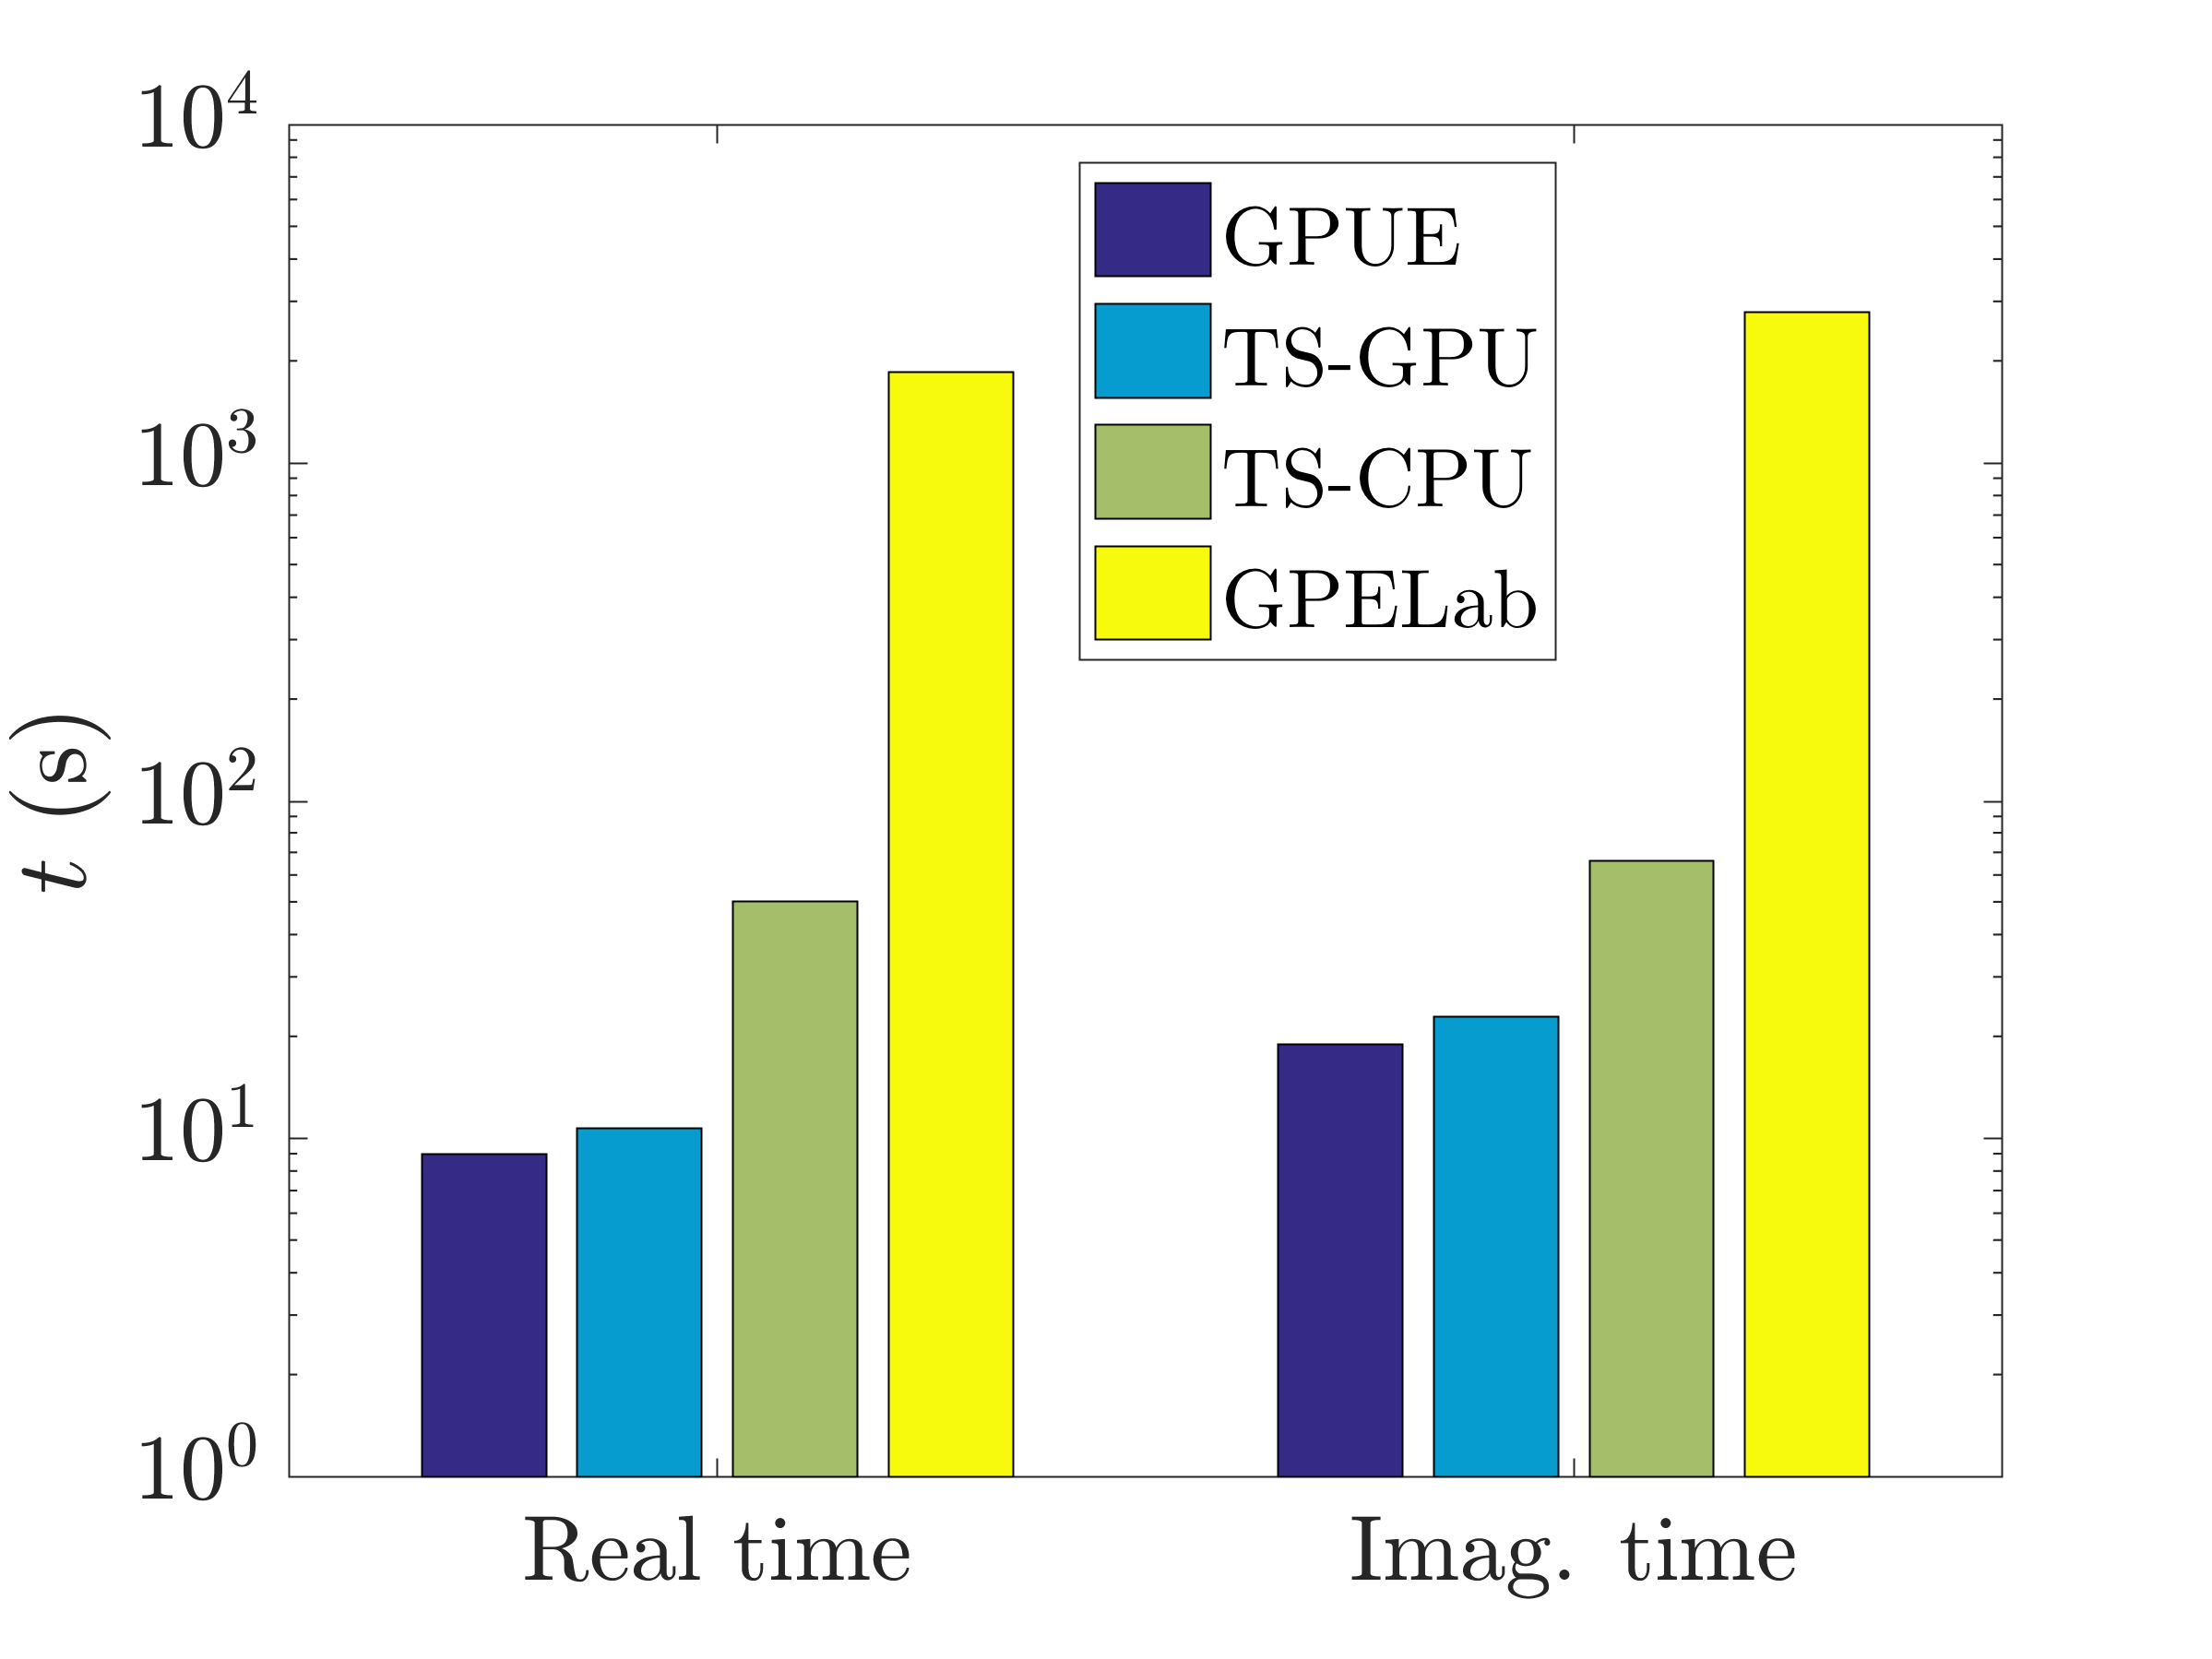
\includegraphics[width=0.7\textwidth,]{ch3_numerics/GPUEvsTS.png}
    \caption{Performance comparison of GPUE and other GPE simulation packages. Data adapted from [wittek url].}
    \label{fig:gpuevsts}
\end{figure}

A simplified sequence and state diagram combination is given in Fig.~\ref{gpue_seq} which describes the operating process for GPUE.

\begin{figure}[h]
    \centering
        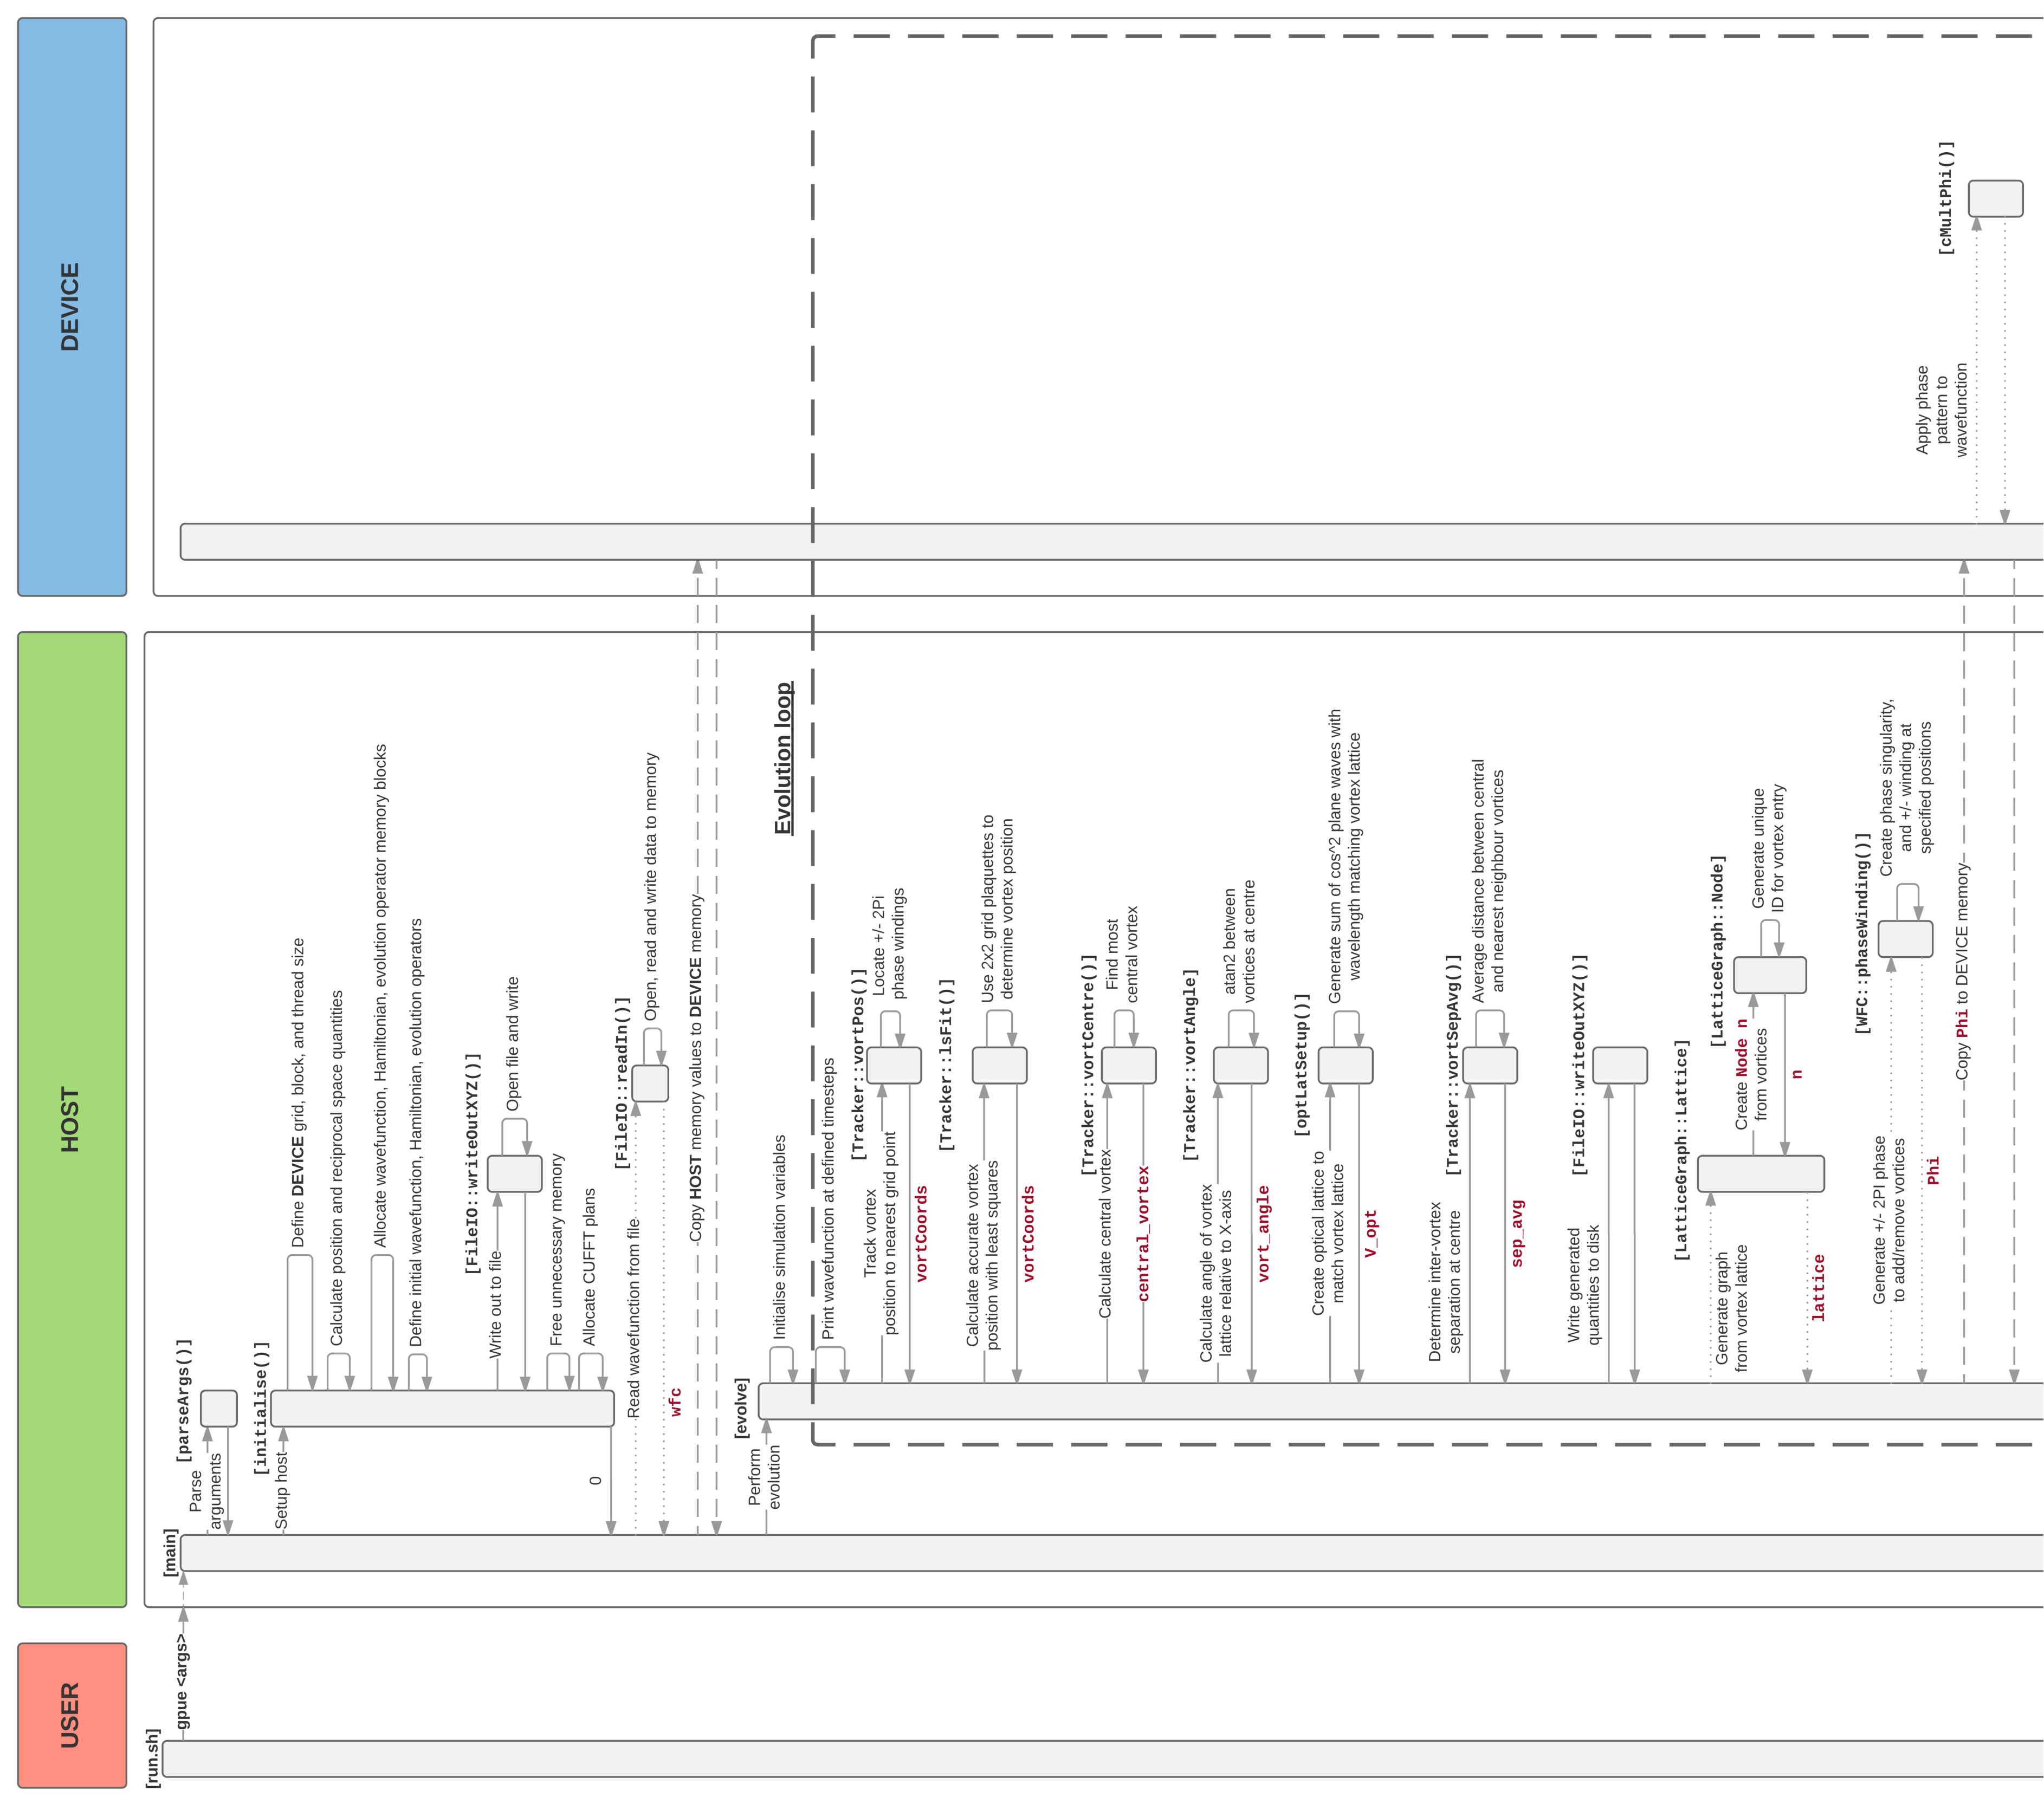
\includegraphics[height=\textwidth,angle=270]{ch3_numerics/GPUE_Seq1}
    \caption{Simplified combined sequence and state diagram for GPUE operation (1 of 2).}
    \label{fig:gpue_seq}
\end{figure}
\begin{figure}[h]
    \centering
        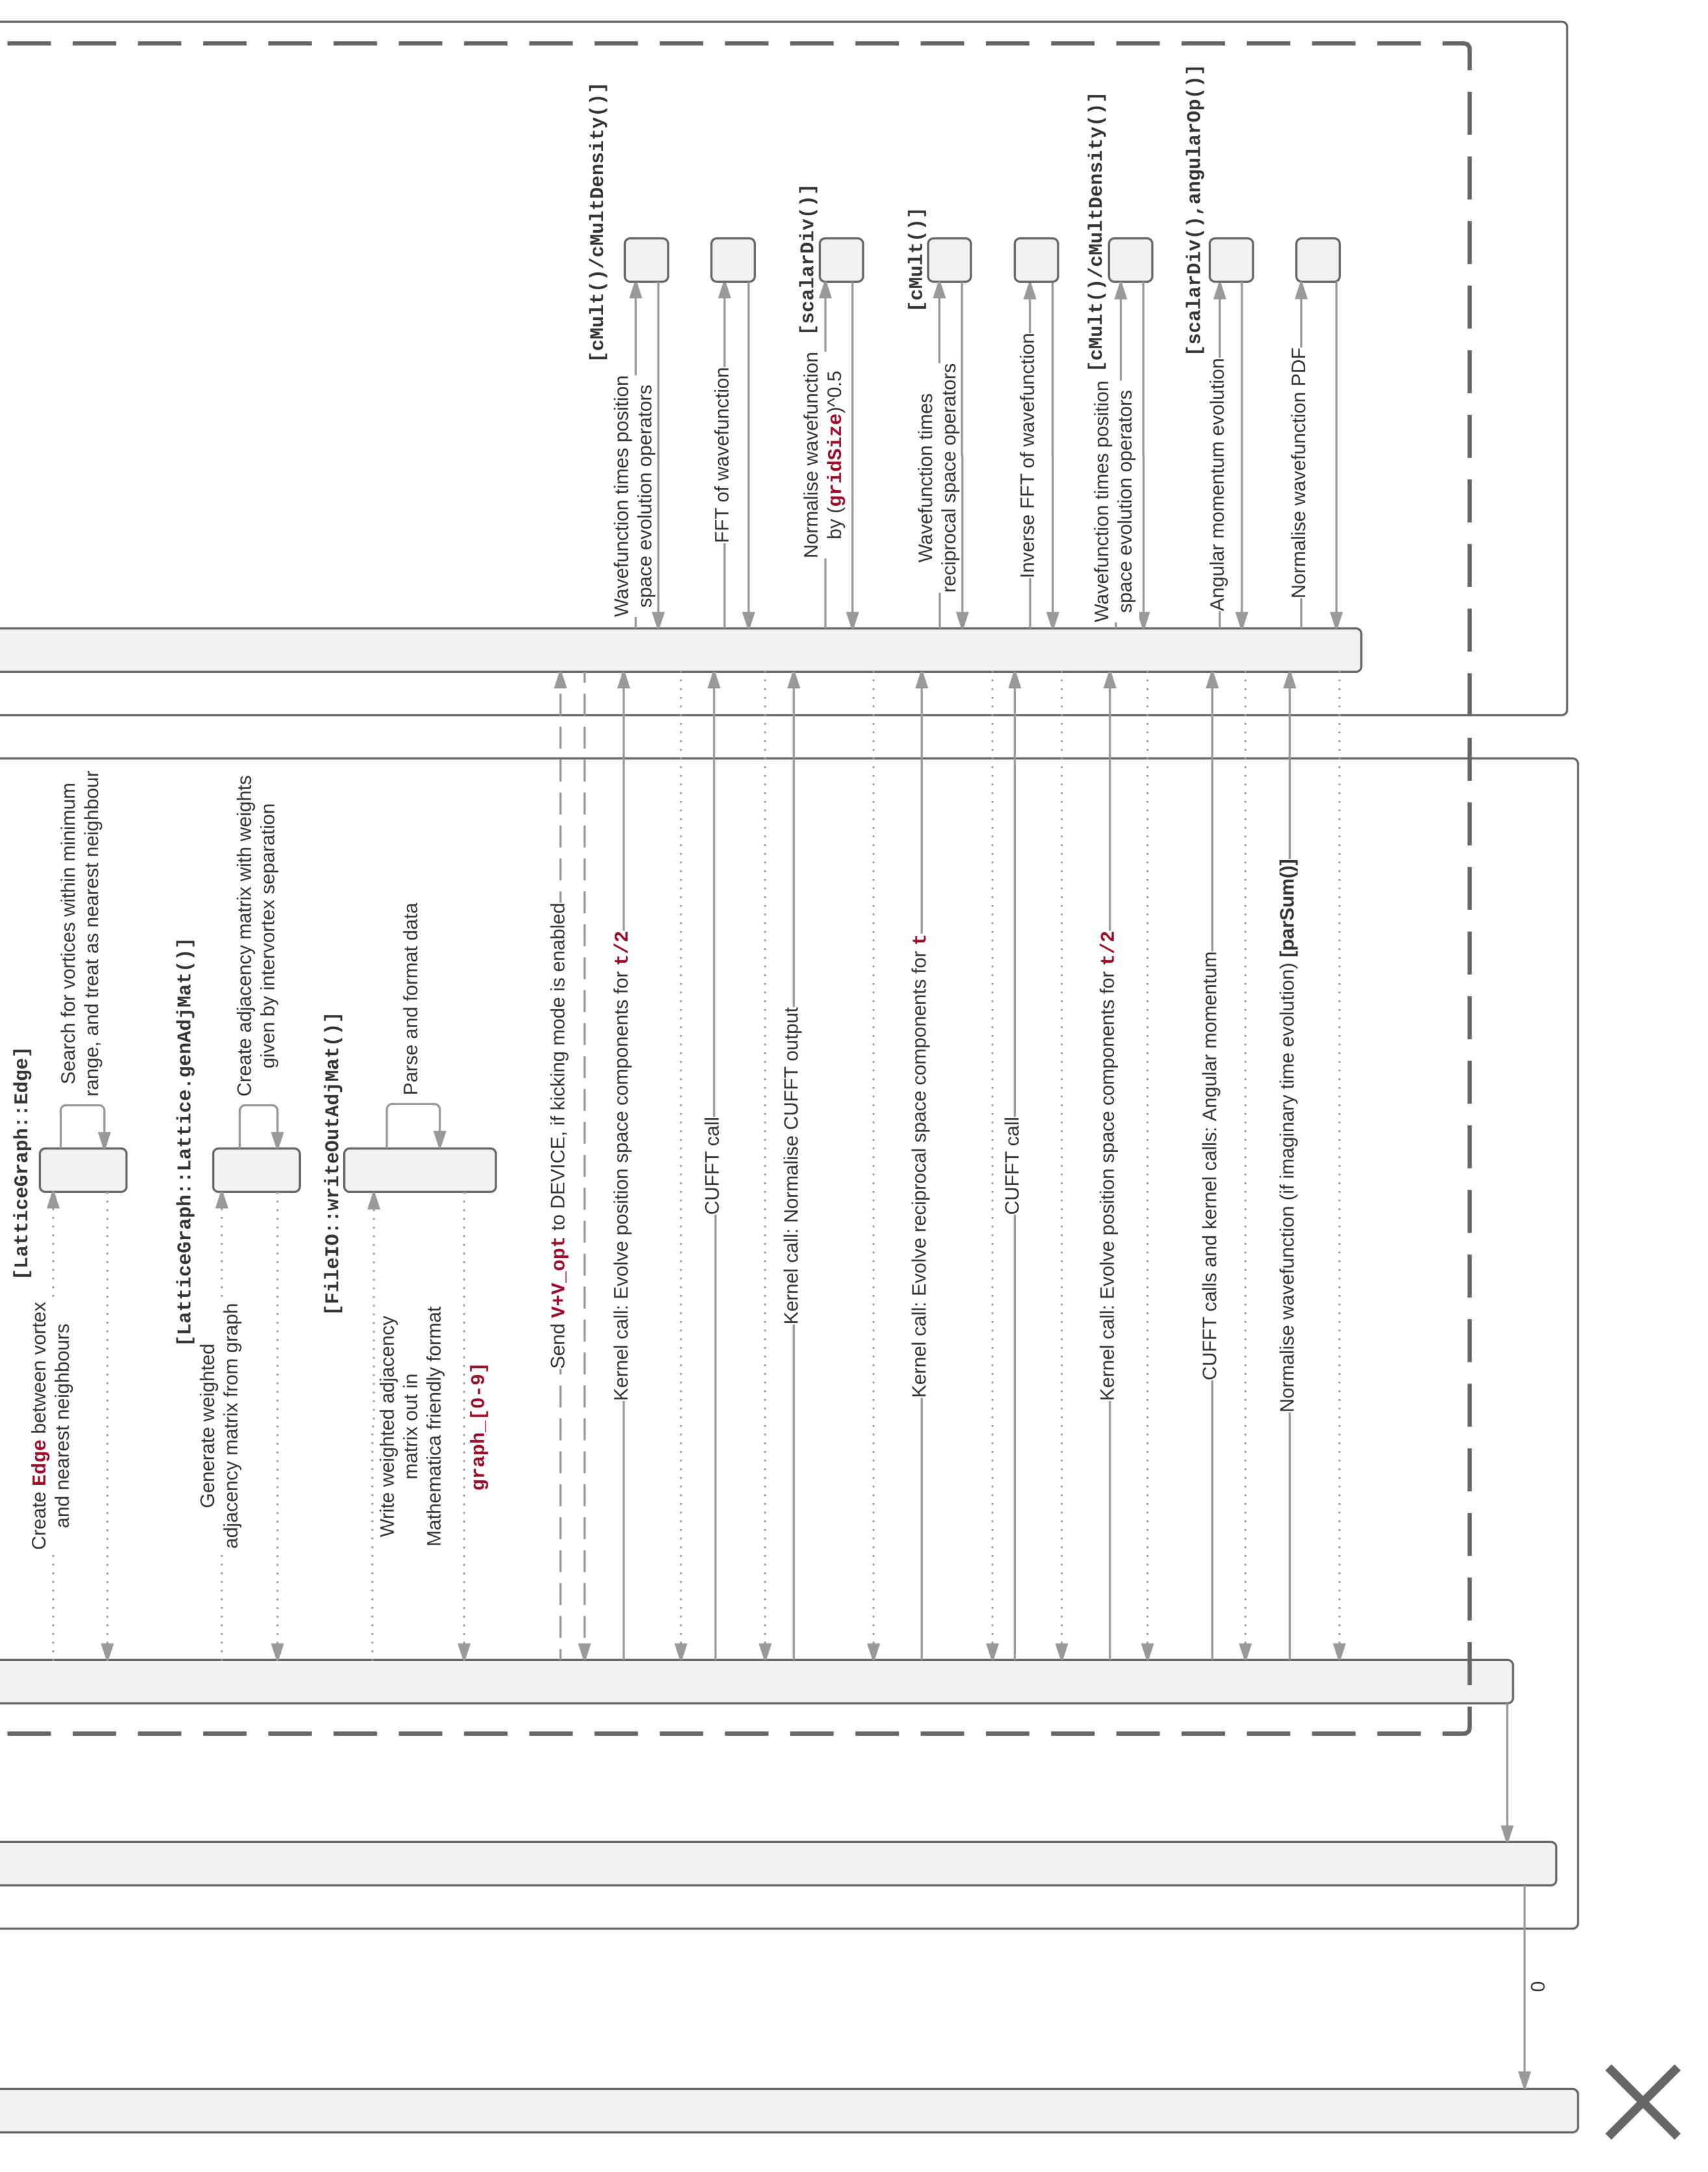
\includegraphics[height=\textwidth,angle=270]{ch3_numerics/GPUE_Seq2}
    \caption{Simplified combined sequence and state diagram for GPUE operation (2 of 2).}
    \label{fig:gpue_seq}
\end{figure}

\subsection{Angular momentum operators using Fourier split-operator (FSO) method}
In the presence of large values of angular momentum, the condensate wavefunction will accommodate many vortices. To ensure a well ordered lattice, it is insufficient to numerically solve the GPE at the required rotation rate. Assuming an initial Gaussian guess, the large number of vortices will enter the condensate from the edge and compete for lattice sites to form the expected Abrikosov pattern. Given the finite resolution and highly degenerate nature of the Abrikosov vortex lattice, it can take a significantly long time to reach and ordered state close to the transverse trapping frequency [Physical
Review Letters, 88(18):180403, (2002)]. Thus, to overcome this issue, I chose to follow the groundstate of the condensate with a ramp of the rotation rate. This is essentially adiabatic evolution during imaginary time, and for all required rotation rates of the condensate we get a vortex lattice ground-state. To allow for this we must examine the behaviour of the angular momentum operators within the FSO algorithm.

The FSO method described earlier works well in handling cases where the operators live in position or momentum space respectively. However, the angular momentum operators are essentially a combination of both spaces. Taking the angular momentum operator along the $z$-axis, $L_z = xp_y - yp_x$, to apply it to the wavefunction requires each basis elements be in the correct space, given the mixed dependencies. For applying this operator we must Fourier transform along a single dimension, multiply by the respective $\mathbf{k}$-space component, take the inverse, multiply by the respective $\mathbf{r}$-space component, and then perform this operation along the other dimensions, summing the results.

This approach accrues an error not encountered using methods solely in position or momentum space. The error can be determined by checking the commutativity of the respective components of the angular momentum operator as

 \begin{subequations}
 \begin{align}
 	\alpha_1 = [x p_y,-y p_x] &= [x p_y,-y] p_x  -  y[x p_y,p_x], \\
 				   &= -[-y,x p_y] p_x + y [p_x, x p_y], \\
 				   &= -\left( {\cancelto{0}{[-y,x]}} p_y + x [-y,p_y] \right) p_x + y \left( [p_x,x] p_y + x {\cancelto{0}{[p_x,p_y]}} \right), \\
 				   &= -x {\cancelto{i\hbar}{[-y, p_y]}} p_x + y {\cancelto{-i\hbar}{[p_x,x]}} p_y, \\
 				   &= -i\hbar \left(x p_x + y p_y \right).
 \end{align}
\end{subequations}

 The complex error term can be seen as, in the case of the implemented evolution, allowing the angular momentum operator to change from imaginary time to real-time, and vice-versa in each respective case. To overcome this, we simply swap the application order of the operator components, between even and odd steps during the evolution. Starting with the alternate order we obtain a value of $\alpha_2 = [-y p_x, x p_y] = i\hbar \left(x p_x + y p_y \right)$. Since we are applying these operators to the condensate we can overcome the error of one term by the application of the other, as
 \begin{equation}
 \exp{i \alpha_1}\exp{i \alpha_2} = 1.
 \end{equation}

 Although alternating will provide a cancellation of this error, it can be assumed that for large timesteps the error will have a non-insignificant contribution to the overall dynamics, as the wavefunction evolves from timestep to timestep. Thus, for this method to remain accurate we can perform the previous decomposition for a second-order accurate scheme.

 A sample wavefunction at a rotation of $\Omega = 0.995\omega_x$ is given by Fig.~\ref{fig:showingoff} showing the density and phase at a resolution of $2^{11}\times 2^{11}$. Although aliasing may be apparent in the phase, this is more likely due to the limited resolution of the computer monitor (printer).

 \begin{figure}
     \centering
     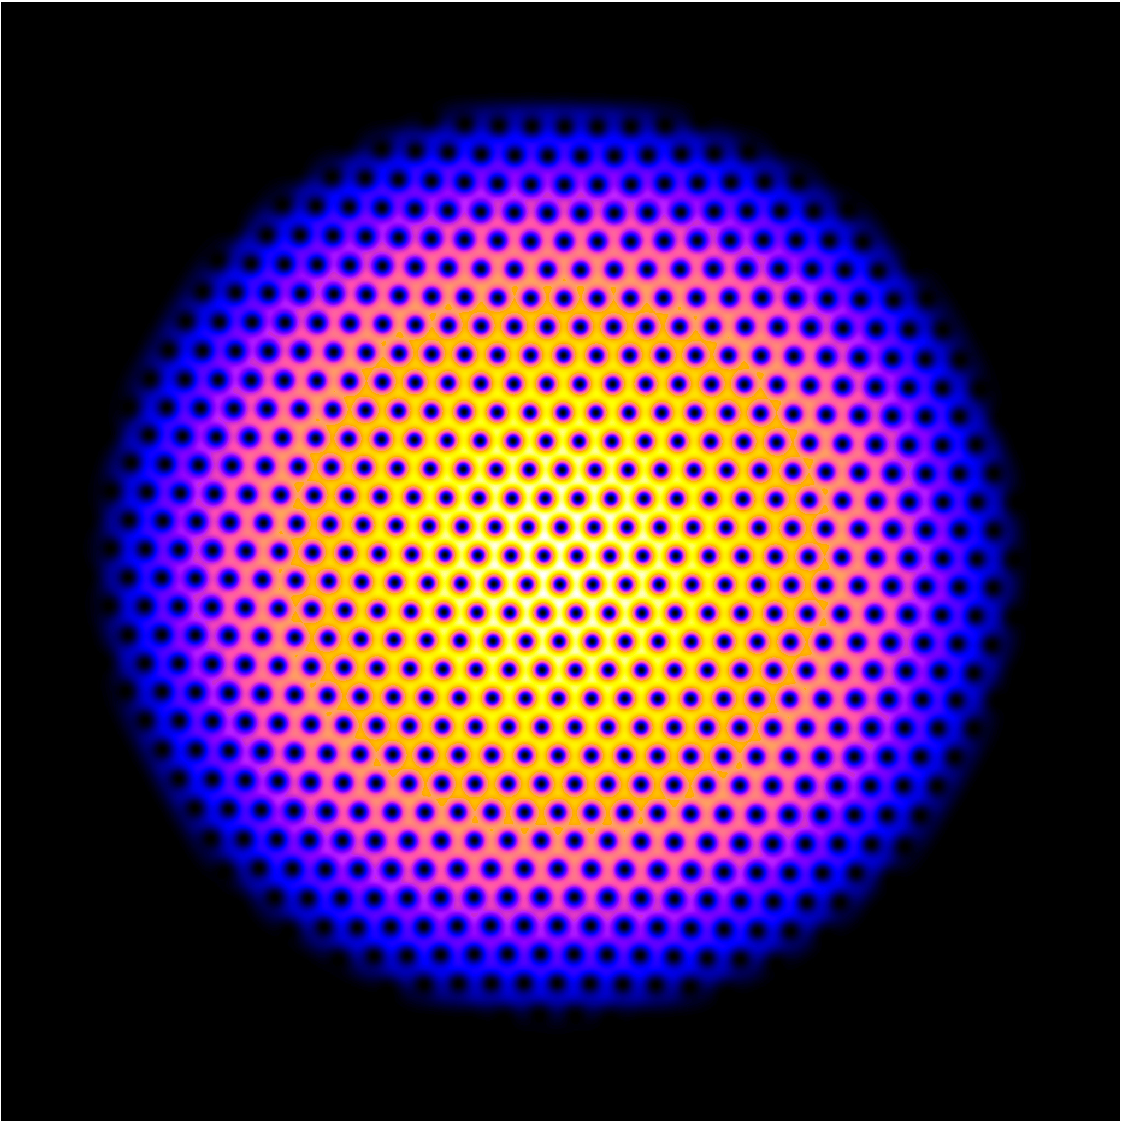
\includegraphics[width=0.45\textwidth,]{ch3_numerics/Rho_995}
     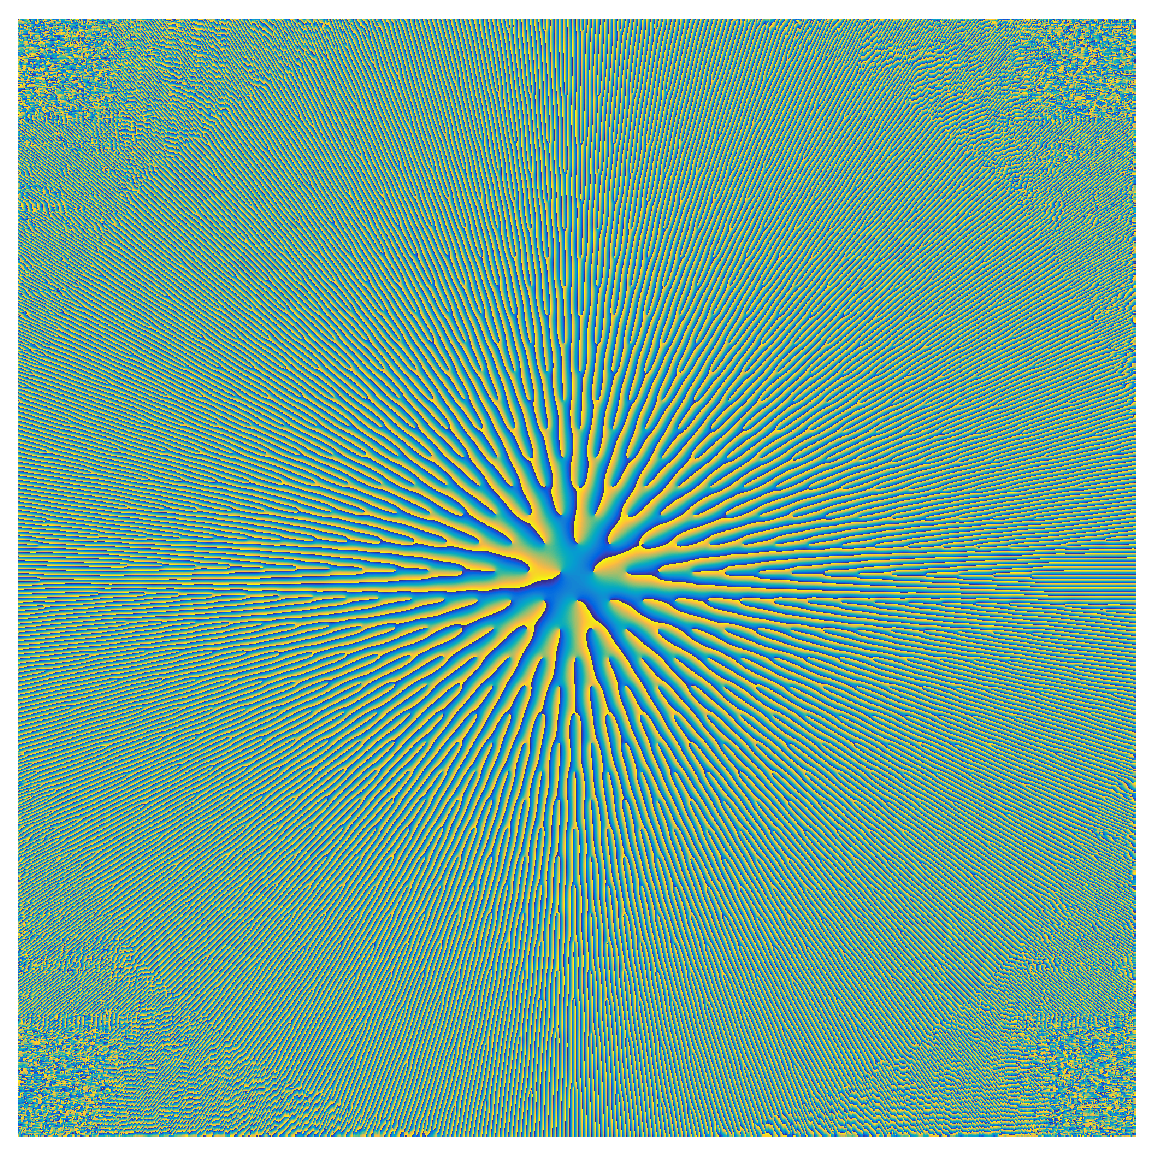
\includegraphics[width=0.45\textwidth,]{ch3_numerics/phi_995}
     \caption{Condensate density (L) and phase (R) at a rotation rate of $\Omega=0.995\omega_x$ for a $2^{11}\times 2^{11}$ grid showing approximately 600 vortices in the visible density regions.}
     \label{fig:showingoff}
 \end{figure}

 \subsection{Vortex tracking}
 To efficiently follow the vortex dynamics, some robust algorithm is needed to track their positions. One could track regions where the density drops to zero. However, this gives very little information on the topological excitation, and may mistake density dips such as phonons for the presence of such excitations. One of the most effective ways is to locate the $\pm 2\pi$ charge in the wavefunction phase, which is a signature of quantum vortices. We can assume that around a $2\times 2$ subgrid, the phase rotates from $-\pi$ to $+\pi$ in the presence of a vortex located on the subgrid. After an initial pass to determine the vortex locations closest the nearest grid element, a least-squares fit is performed to more accurately determine the vortex core position.

 Linear least squares is used generally for an overdetermined linear system $\mathbf{A}\mathbf{r} = \mathbf{b}$, where unique solutions are unlikely to exist. Thus, for a solution, we seek the best fit plane that minimises the error, of the form

 \begin{equation}
 S(\mathbf{r}) = \displaystyle\sum |b_i - \displaystyle\sum A_{ij} r_j |^2
 \end{equation}
 where $S$ is the objective function to be minimised, following $\mathbf{b} = \argmin S(\mathbf{r})$. The solution of this minimisation problem is given by
 \begin{subequations}
\begin{align}
    \mathbf{A} ^{T}\mathbf{A} \mathbf{r} &= \mathbf{A} ^{T}\mathbf{b}, \\
    \mathbf{r} &= (\mathbf{A}^{T}\mathbf{A})^{-1}\mathbf{A}^{T}\mathbf{b}.
\end{align}
\end{subequations}
For this the best-fit plane is sought of the form
$a_0 c + \displaystyle\sum\limits_{i}^{m} a_i r_i = f(\mathbf{r})$
which for a two-dimensional system, $\mathbf{r} = \{x,y\}$, is given by the matrix,
\begin{equation}
    \mathbf{A} = \left(
    \begin{array}{ccc}
        0 & 0 & 1 \\
        0 & 1 & 1 \\
        1 & 0 & 1 \\
        1 & 1 & 1
    \end{array}\right).
\end{equation}
The above matrix is composed of all possible planes that can fit over a square $2\times 2$ grid plaquette,
and
\begin{equation}
    \mathbf{b} = \left(
    \begin{array}{cccc}
        \Psi(x_0,y_0) & \Psi(x_0,y_1) & \Psi(x_1,y_0) & \Psi(x_1,y_1)
    \end{array} \right)^{T},
\end{equation}
are the wavefunction values around the sampled $2\times 2$ grid.
Upon evaluating the vector $\mathbf{r}$ above, one can obtain the best fit plane  solution as
\begin{equation}\left(
    \begin{array}{c}
        x \\
        y \\
        c
    \end{array}\right)
    = \left(
    \begin{array}{c}
        0.5( -\Psi(x_0,y_0) + \Psi(x_0,y_1) - \Psi(x_1,y_0) + \Psi(x_1,y_1) ) \\
        0.5( -\Psi(x_0,y_0) - \Psi(x_0,y_1) + \Psi(x_1,y_0) + \Psi(x_1,y_1) ) \\
        3\Psi(x_0,y_0) + \Psi(x_0,y_1) - \Psi(x_1,y_0) - \Psi(x_1,y_1) )
    \end{array}\right).
\end{equation}

The goal is to find where both the real and imaginary components cross through zero, and thus we seek a solution of the form $x + y = -c$. Rearranging the above equations as
\begin{equation}\left(
    \begin{array}{cc}
        \Re(x) & \Re(y) \\
        \Im(x) & \Im(y) \\
    \end{array}\right)
    \left(
    \begin{array}{c}
        \delta x \\
        \delta y
    \end{array}\right)
    =
    \left(
    \begin{array}{c}
        \Re(c)
        \Im(c)
    \end{array}\right).
\end{equation}
and again solving the linear system by inverting the left-hand matrix and multiplying across allows one to seek the corrections to the vortex position, $\delta \mathbf{r} = \{\delta x, \delta y \}$.

 With this, we can accurately determine the motion of the vortices with high precision. To track the vortices during the evolution, the creation of an initial list of vortices is performed, with each given a unique identifier. Assuming the vortex cores can travel a limited distance (some multiple of the grid resolution) between time steps, we can say at subsequent times which vortex has moved to the newly found positions.

 This is performed through representing vortices as a graph, each with an assigned unique identifier, associated location, phase winding and on/off flag. Edges are created between vortices that are separated by at most root-two the average of the inter-vortex spacings. A finite boundary is chosen to examine only vortices at the center, which can cause vortices to appear and disappear on the boundary. Thus, any vortex which appears without association to an initial vortex, or any vortex that leaves the boundary, is switched off and remains so for all analysis.

        \section{Numerical implementation of the Bogoliubov-de Gennes equations (Appendix?)}
In section \ref{bogo deriv}, I have shown the BdG equations, which are used to examine the stability of a state in BECs. To solve the Bogoliubov equations numerically requires searching for the solution to a generalised non-Hermitian eigenvalue problem. Thus, the system must be formally specified in matrix form. The derivative operators of $H_0$ are specified using second-order central differences, represented by
\begin{equation}
    \partial^2_i = \frac{U_{i+1,j} + U_{i-1,j} - 2U_{i,j}}{h^2}
\end{equation}
where $i$ is the respective dimension for the derivative, and $h$ is the step size. In matrix form, this becomes
\begin{equation}
    \mathbf{B} =
    \begin{bmatrix}
            -2      &   1    &    0   &  \cdots   &  \cdots   &  \cdots   & 0 \\
            1       &   -2   &    1   &           &           &     &  \vdots \\
            0       &    1   &   -2   & \ddots    &           &     &  \vdots \\
            \vdots  &        & \ddots & \ddots    & {\ddots}  &     &  \vdots \\
            \vdots  &        &        & \ddots    &    -2     &  1  &       0 \\
            \vdots  &        &        &           &     1     & -2  &       1 \\
            0       & \cdots & \cdots & \cdots    &     0     &  1  &      -2 \\
        \end{bmatrix}.
\end{equation}
where the number of rows and columns equal the number of elements along the dimension to be differentiated. To construct a multidimensional version, we take a Kronecker sum of the matrix $B$ along each respective dimension of the system. This can be represented as
\begin{equation}
    \mathbf{B}_{i,j} = \mathbf{B}_i \oplus \mathbf{B}_j = \mathbf{B}_i \otimes \mathbf{I}_j + \mathbf{I}_i \otimes \mathbf{B}_j
\end{equation}
were $i,j$ are the indices of the respective dimensions, and $\mathbf{I}$ is the identity equal in size to dimensions $i,j$. With this operation, we can obtain a block diagonal matrix that represents the laplacian operator as

\begin{equation}
    \nabla^2=
    \begin{bmatrix}
        \mathbf{B}    & \mathbf{I} &      0      &  \cdots      &      0       \\
        \mathbf{I}    & \mathbf{B} &  \ddots     &              &  \vdots      \\
        0             & \ddots     &  \ddots     &  \ddots      &      0       \\
        \vdots        &            &  \ddots     &  \ddots      &  \mathbf{I}  \\
        0             & \cdots     &      0      &  \mathbf{I}  &  \mathbf{B}
    \end{bmatrix}.
\end{equation}

Similarly, the angular momentum operator $L_z = i\hbar(x\partial_y + y\partial_x$ can be defined in terms of first derivative matrices. The non-derivative operators require a reshaping into lexicographical indexing ($N$-d to 1-D), and will sit along the diagonal. As these systems have many more 0's than elements, it makes sense to store them in a sparse matrix format. Given the proposed system is not Hermitian, a generalised eigenvalue solver is required. For the sake of simplicity, these systems can be solved in MATLAB, using \textit{eigs}, which makes use of the Arnoldi (non-Hermitian) or Lanczos (Hermitian) algorithm for finding the specified number of eigenvectors and values.

        \section{Angular momentum operators using Fourier split-operator method}

Given that in the presence of large values of angular momentum, the condensate wavefunction will accommodate many vortices. To ensure a well ordered lattice, it is insufficient to numerically solve the GPE at the required rotation rate. Assuming an initial Gaussian guess, the large number of vortices will enter the condensate from the edge and compete for lattice sites to form the expected Abrikosov pattern. Thus, to overcome this issue, following the groundstate of the condensate with a ramp of the rotation rate is often necessary. This is essentially adiabatic evolution during imaginary time, and for all required rotation rates of the condensate we get a vortex lattice ground-state. To allow for this we must examine the behaviour of the angular momentum operators within the FSO algorithm.

The Fourier split-operator method described earlier works well in handling cases where the operators live in position or momentum space respectively. However, the angular momentum operators are essentially a combination of both spaces. Taking the angular momentum operator along the $z$-axis, $L_z = xp_y - yp_x$, and applying it to the wavefunction requires each basis elements be in the correct space, given the mixed dependencies. Thus, to apply this operator we must Fourier transform along a single dimension, multiply by the $\mathbf{k}$-space operator, take the inverse, multiply by the $\mathbf{r}$-space operator, and then perform this operation along the other dimension, summing the results.

 This mixed phase approach accrues an error not encountered using methods solely in position or momentum space. The error can be determined by checking the commutativity of the respective components of the angular momentum operator as

 \begin{subequations}
 \begin{align}
 	L_1 = [x p_y,-y p_x] &= [x p_y,-y] p_x  -  y[x p_y,p_x], \\
 				   &= -[-y,x p_y] p_x + y [p_x, x p_y], \\
 				   &= -\left( {\cancelto{0}{[-y,x]}} p_y + x [-y,p_y] \right) p_x + y \left( [p_x,x] p_y + x {\cancelto{0}{[p_x,p_y]}} \right), \\
 				   &= -x {\cancelto{i\hbar}{[-y, p_y]}} p_x + y {\cancelto{-i\hbar}{[p_x,x]}} p_y, \\
 				   &= -i\hbar \left(x p_x + y p_y \right).
 \end{align}
\end{subequations}

 The complex error term can be seen as, in the case of the implemented evolution, allowing the angular momentum operator to change from imaginary time to real-time, and vice-versa in each respective case. To overcome this, we simply swap the application order of the operator components, between even and odd steps during the evolution. Starting with the alternate order we obtain a value of $L_2 = [-y p_x, x p_y] = i\hbar \left(x p_x + y p_y \right)$. Since we are applying this phase to the condensate we can overcome the error of one term by the application of the other, as
 \begin{equation}
 \exp{i L_1}\exp{i L_2} = 1.
 \end{equation}

 Although alternating will provide a cancellation of this error, it can be assumed that for large timesteps the error will have a non-insignificant contribution to the overall dynamics, as the wavefunction evolves from timestep to timestep. Thus, for this method to remain accurate we can perform the previous decomposition for a second-order accurate scheme.

 \section{Vortex tracking}
 To efficiently follow the vortex dynamics, some robust algorithm is needed to track their positions. One could track regions where the density drops to zero. However, this gives very little information on the topological excitation, and may mistake density dips such as phonons for the presence of such excitations. One of the most effective ways is to locate the $\pm 2\pi$ charge in the wavefunction phase, which is a signature of quantum vortices. We can assume that around a $2\times 2$ subgrid, the phase rotates from $-\pi$ to $+\pi$ in the presence of a vortex located on the subgrid. After an initial pass to determine the vortex locations closest the nearest grid element, a least-squares fit is performed to more accurately determine the vortex core position.


 Linear least squares is used generally for an overdetermined linear system $\mathbf{A}\mathbf{x} = \mathbf{b}$, where unique solutions are unlikely to exist. Thus, for a solution, we seek the best fit plane that minimises the error, of the form

 \begin{equation}
 S(\mathbf{x}) = \displaystyle\sum |b_i - \displaystyle\sum A_{ij} x_j |^2
 \end{equation}
 where $S$ is the objective function to be minimised, following $\mathbf{b} = \argmin S(\mathbf{x})$. The solution of this minimisation problem is given by
 \begin{subequations}
\begin{align}
    \mathbf{A} ^{T}\mathbf{A} \mathbf{x} &= \mathbf{A} ^{T}\mathbf{b} \\
    \mathbf{x} &= (\mathbf{A}^{T}\mathbf{A})^{-1}\mathbf{A}^{T}\mathbf{b}
\end{align}
\end{subequations}
and assuming a plane of the form $x + y + c = f(x,y)$,
\begin{equation}
    \mathbf{A} = \left(
    \begin{array}{ccc}
        0 & 0 & 1 \\
        0 & 1 & 1 \\
        1 & 0 & 1 \\
        1 & 1 & 1
    \end{array}\right),
\end{equation}
and
\begin{equation}
    \mathbf{b} = \left(
    \begin{array}{cccc}
        \Psi(x_0,y_0) & \Psi(x_0,y_1) & \Psi(x_1,y_0) & \Psi(x_1,y_1)
    \end{array} \right)^{T},
\end{equation}
are the wavefunction values around the sampled $2\times 2$ grid.
Upon evaluating the vector $\mathbf{x}$ above, one can obtain the best fit plane  solution as
\begin{equation}\left(
    \begin{array}{c}
        x \\
        y \\
        c
    \end{array}\right)
    = \left(
    \begin{array}{c}
        0.5( -\Psi(x_0,y_0) + \Psi(x_0,y_1) - \Psi(x_1,y_0) + \Psi(x_1,y_1) ) \\
        0.5( -\Psi(x_0,y_0) - \Psi(x_0,y_1) + \Psi(x_1,y_0) + \Psi(x_1,y_1) ) \\
        3\Psi(x_0,y_0) + \Psi(x_0,y_1) - \Psi(x_1,y_0) - \Psi(x_1,y_1) )
    \end{array}\right).
\end{equation}

The goal is to find where both the real and imaginary components cross through zero, and thus we seek a solution of the form $x + y = -c$. Arranging the above equations into matrix form as
\begin{equation}\left(
    \begin{array}{cc}
        \Re(x) & \Re(y) \\
        \Im(x) & \Im(y) \\
    \end{array}\right)
    \left(
    \begin{array}{c}
        \delta x \\
        \delta y
    \end{array}\right)
    =
    \left(
    \begin{array}{c}
        \Re(c)
        \Im(c)
    \end{array}\right).
\end{equation}
and again solving the linear system by inverting the left-hand matrix and multiplying across allows one to seek the corrections to the vortex position, $\delta \mathbf{r} = \{\delta x, \delta y \}$.


 With this, we can accurately determine the motion of the vortices with high precision. To track the vortices during the evolution, the creation of an initial list of vortices is performed, with each given a unique identifier. Assuming the vortex cores can travel a limited distance (some multiple of the grid resolution) between time steps, we can say at subsequent times which vortex has moved to the newly found positions.

 This is performed through representing vortices as a graph, each with an assigned unique identifier, associated location, phase winding and on/off flag. Edges are created between vortices that are separated by at most root-two the average of the inter-vortex spacings. A finite boundary is chosen to examine only vortices at the center, which can cause vortices to appear and disappear on the boundary. Thus, any vortex which appears without association to an initial vortex, or any vortex that leaves the boundary, is switched off and remains so for all analysis.


    %%\section{Error analysis}
%ignore?

\fi
%%%%%%%%%%%%%%%%%%%%%%%%%%%%%%%%%%%%%%
\newif\ifvtxdyn
\vtxdyntrue
\ifvtxdyn
    \chapter{Bose-Einstein condensate dynamics}
        %\chapter{Bose--Einstein condensate dynamics}
\section{Condensate dynamics}
With the background theory outlined in Sections~\ref{sec:superfluid,sec:coldatoms}, I will now discuss manipulations and dynamics of the condensate. Due to phase coherence over all atoms, we can say that any perturbation to the condensate phase will (given sufficient time), have some affect on all condensed atoms. Direct manipulation of the phase is interesting as the condensate phase encapsulates all quantum behaviour of the system. Secondly, given the phase term is, following Eq.~\ref{eqn:madelung}, modifiable to any arbitrary values (within the range $\pm \pi$).

Also, with the condensate velocity determined by Eq.~\ref{eqn:velocity}, it is possible, upon engineering of the condensate phase, to control the atomic velocity. This opens an interesting set of possibilities as control of the phase, and hence velocity, allows for development of a wide range of quantum states and dynamics.



\section{Rapidly rotating vortex lattice}
Given the need for a well ordered vortex lattice it is instructive to discuss the generation of such a system. I assume an initial wavefunction guess of a two-dimensional gaussian having some finite overlap with the groundstate of the system in the absence of angular rotation. Following an imaginary time-evolution like what was outlined in Sec.~\ref{sec:numerics}, the groundstate of the condensate is found.



\section{Phase imprinting and manipulation}
Writing the wavefunction in the standard Madelung transform form, alongside a phase imprint term $\phi$ is given as
\begin{equation}
    \Psi(\mathbf{r},t) = |\Psi(\mathbf{r},t)|e^{\text{i}(\theta(\mathbf{r},t) + \phi(\mathbf{r}))}.
\end{equation}


%%% TO BE MOVED IN WITH PHASE ENGINEERING
Following \cite{BK:Pitaevskii_Stringari_2003} and taking the Madelung transform of the wavefunction given by Eq. \eqref{eqn:madelung}, the phase of the condensate may be specified as
\begin{equation}
\theta = \theta_c + \theta_i,
\end{equation}
where $\theta_c$ is the unperturbed condensate phase, and $\theta_i$ is the phase pattern to be imprinted. Thus, upon solving for the initial condensate phase, an additional phase pattern can be imprinted at any time by multiplying the wavefunction by the intended phase pattern. This is in line with the phase imprinting method, as previously introduced by Dobrek \textit{et al}. \cite{Vtx:Dobrek_pra_1999}.
%%% TO BE MOVED IN WITH PHASE ENGINEERING



\subsection{Gaussian phase}

\subsubsection{One dimensional}

\subsubsection{Two dimensional}



\section{Few vortex states}
As discussed in Section~\ref{sec:superfluid}, the discovery and manipulation of quantum vortices remains an active area of research.







Given that the energy of a vortex-carrying condensate scales as $E\propto l^2$, as $L_z \propto l$, any increase in the angular momentum causes a squared increase in the energy. Thus, for energetic favorability, the system prefers to maintain singly-charged vortices. To generate a vortex in the condensate costs energy,

Wi

\section{Quantum vortex dynamics}



\section{Vortex lattice states}
    \begin{equation}
        E(\Psi) = \int \Psi^{*} H_{\text GP} -\Omega L_z \Psi
    \end{equation}

    \fi
%%%%%%%%%%%%%%%%%%%%%%%%%%%%%%%%%%%%%%
\newif\ifmoire
\moiretrue
\ifmoire
    \chapter{Moir\'e superlattice structures}
        %\section{Delta-kick dynamics}
\section{Introduction}

As mentioned in Sec.~\ref{sec:vortlatt}, the use of optical lattice potentials is ubiquitous in the field of ultracold atoms. Given their perfect periodic structure, it is interesting to examine the effect these lattices have on already periodic structures. For a rapidly rotating condensate, the density will feature a large periodic Abrikosov lattice having $6$-fold triangular symmetry. The use of optical lattices on vortex lattices has previously been shown to allow for pinning of the vortex cores to the lattice maxima \cite{OL:Reijnders_prl_2004,Vtx:Tung_prl_2006}. Assuming blue detuned laser fields, the lattice maxima will drive atoms away, and make it favourable for vortex cores to sit in these positions. The observation of a transition between lattice geometries can be observed in these cases. This is, however, experimentally challenging as the optical lattice must rotate with the vortex lattice and match its rotation rate. Nevertheless, the creation of a rotating quasi two-dimensional optical lattice was achieved in~\cite{Vtx:Tung_prl_2006}, where the authors used a rotating mask with the holes placed in such a way as to allow for the required optical diffraction patterns. However, the system suffered from difficulties arising from the inclusion of a mechanically rotating stage, as well as the heating effects due to the presence of the always-on optical lattice. As the vortex lattice has 6-fold rotational symmetry, after rotating by
$\Omega_{k}=6\Omega=2\pi\times 6$ Hz the system has returned to its initial orientation. It is therefore intriguing to see if the need for a rotating optical potential can be replaced by a periodically flashed optical lattice. Here, we will take the first and investigate the effect of a single application of an optical lattice to the vortex lattice.

 For short application times, the potential will kick the wavefunction, and can be seen as leaving a phase imprint with minimal immediate density change. As discussed in Sec.~\ref{ss:pert_opt_latt}, the effect of the kick can then be observed in the ensuing dynamics. Interestingly, one can observe the appearance of moir\'e interference patterns in the condensate density, while the positions of the vortex cores are only minimally affected. We will begin by discussing the model, and present the explanation of the resulting interference pattern. Next, we will show that it stems from the interference between the different $\mathbf{k}$-vectors, with signatures of the effect being visible in the condensate's kinetic energy spectrum. Finally, we will discuss the uses of this effect as a microscope for observing the presence of vortex lattices without time-of-flight.

As already discussed in detail above, given the large number of vortices in the condensate density, as well as the lowered density resulting from large centrifugal forces, the vortex cores become large and form a highly periodic triangular lattice. The non-orthogonal lattice vectors are given in position space by $\mathbf{a}_1 = a_v[1,0]$ and $\mathbf{a}_2 = a_v[-1/2, \sqrt{3}/2]$, where $a_v$ is the distance between vortex cores. The lattice ``constant'' is truly only constant in areas of near uniform density. Thus, due to the inhomogeneous wavefunction density, the vortices near the edges are separated by a much greater distance than those at the centre. For the analysis we have therefore chosen to ignore all vortices near the condensate edge. The momentum space ($\mathbf{k}$-space) lattice vectors are reciprocal to the given $\mathbf{r}$-space vectors, and given by $\mathbf{b}_1 = 4\pi/(\sqrt{3}a_v)[\sqrt{3}/2,1/2]$ and $\mathbf{b}_2 = (4\pi/(\sqrt{3}a_v))[0,1]$.
%[!!!!check for consistency!!!!]

\section{Model}

Using an optical potential one can create a perturbation in the condensate density by switching it on for a brief period of time. Such a {\it kick} must occur only for a time much shorter than the rotation period of the vortex lattice, of angular rotation frequency $\Omega = 0.995\omega_\perp$, so that the effect is limited to a phase imprinting and not to a direct change in the density distribution. For the work carried out herein, the duration of the kick is $\tau_{\text{kick}}=10^{-5}$~s, which is fast compared to the classical rotation period of the 6-fold symmetric lattice of $T_{6} \approx 166 $ ms. This ensures that the vortex lattice is essentially stationary during the kick. To examine the effect that periodicity plays on the system, the optical potential was chosen to match the geometry of the Abrikosov vortex lattice, with the angle of relative alignment $\theta_\Delta$ given as a free parameter. The optical potential was modeled as the sum of counter-propagating laser beams, as
\begin{equation}
    V_{\text{opt}} = V_0\displaystyle\sum_{j}\cos^2 \left[ \textbf{k}_{j}\cdot\textbf{r} \right],
\end{equation}
where $V_0$ is the optical lattice potential amplitude, and $j=\lbrace 0,1,2,\ldots \rbrace$ is the index of each respective laser with a differing $\mathbf{k}$-space wave-vector. By careful choice of the wave-vectors $\textbf{k}_{j}$ the density modulation given by the vortices is matched to the optical potential. This is achieved using the reciprocal lattice vectors defined by the vortex lattice, $\mathbf{b}_{1,2}$, and an additional third wave-vector, $\mathbf{k}_3 = 4\pi/(\sqrt{3}a_o)\{\sqrt{3}/2,-1/2\}$. For the resulting optical potential, we define the lattice sites as the maxima of intensity. These, which are in turn matched with the condensate density minima of the vortex lattice.


As the vortex lattice constant in a rapidly rotating atomic BEC is large, optical lattices with wavelengths on the order of tens of microns are necessary \cite{BEC:Fallani_optexp_2005, AO:Williams_optexp_2008}. By ensuring a short kick with an amplitude on the order of $10^{-2} \mu $, with $\mu$ as the BEC's chemical potential, the result of the kick is an imprinted phase on the wavefunction \cite{Vtx:Dobrek_pra_1999}. As an example, following a single kick the vortex lattice phase can be observed to be modified, with localised phase gradients at the optical lattice maxima, as seen in Fig.~\ref{fig:Phase_diff_after_kick}. These localised gradients lead to the development of a flow originating from each optical lattice potential maxima location, and in turn create well-defined interference patterns resulting from phonons created by the kick. In the presence of a vortex lattice with a periodic core arrangement, this creates moir\'e superlattice structures \cite{SS:Murata_acsn_2010} in the density of the condensate. This type of pattern has been observed in many solid-state systems, such as graphene on hexagonal boron nitride~\cite{SS:Yankowitz_natphys_2012}, though it is static in such cases. In this system, the structures are dynamical, and revive at well defined intervals.

\begin{figure}
    \centering
    \includegraphics[width=0.95\textwidth]{ch5_kickit/Phase_diff_after_kick}
    \caption[Phase modulation following a kick.]{The condensate phase for the vortex lattice following a kick (left) and without the background lattice phase at $t=0$ (right). The phase modulation through the optical lattice kick is clearly visible.}
    \label{fig:Phase_diff_after_kick}
\end{figure}


%%%Spectral
\iffalse
To study these resulting structures, we have performed a spectral decomposition of the kinetic energy of the condesate~\cite{CT:Nore_prl_1997,CT:Nore_pof_1997,CT:Bradley_prx_2012}. For this the wavefunction is first written in amplitude (density) $\rho(\mathbf{r},t)$ and phase $S(\mathbf{r},t)$ form via a Madelung transform as given by \eqref{eqn:madelung}.
\iffalse
as
$
		\Psi(\mathbf{r},t) = \sqrt{\rho(\mathbf{r},t)}\exp{\left[\mathrm{i}S(\mathbf{r},t)\right]}.
$
\fi
Making use of the Gross--Pitaevskii energy functional \eqref{eqn:gpe_functional}, and substituting in the above form gives
\begin{equation}
    E_{\text{kqp}} = \int d\mathbf{r} \left( \frac{\hbar^2}{2m}| \nabla\sqrt{\rho(\mathbf{r},t)} |^2  + \frac{m}{2}|\sqrt{\rho(\mathbf{r},t)}\mathbf{v}(\mathbf{r},t) |^2\right).
\end{equation}
One can decompose this into the quantum pressure (first) and kinetic energy (second) terms. The kinetic energy term can seen as a density-weighted velocity field, $\mathbf{u}(\mathbf{r},t) = \sqrt{\rho(\mathbf{r},t)}\mathbf{v}(\mathbf{r},t)$. This can be further decomposed into the sum of compressible and incompressible terms,
\begin{equation}\label{eqn:kin_en}
    \mathbf{u(r},t) = \mathbf{u}^c(\mathbf{r},t) + \mathbf{u}^i(\mathbf{r},t),
\end{equation}
where $\mathbf{u}^c, \mathbf{u}^i$ are the compressible and incompressible terms respectively. This can be solved for both terms by performing a Helmholtz decomposition on the resulting field separating terms that are longitudinal ($\mathbf{u}^c$) and transverse ($\mathbf{u}^i$) with
\begin{subequations}\label{eqn:kinterms}
\begin{align}
    \nabla \times \mathbf{u}^c(\mathbf{r},t) = 0, \\
    \nabla \cdot \mathbf{u}^i(\mathbf{r},t) = 0.\\
\end{align}
\end{subequations}
By introducing the vector potential, $\mathbf{A}$, and scalar potential, $B$, such that
\begin{subequations}
\begin{align}
    \mathbf{u}^c = \nabla B, \\
    \mathbf{u}^i = \nabla \times \mathbf{A} \\
\end{align}
\end{subequations}
we can rewrite Eq.~\eqref{eqn:kin_en} as
\begin{align}
    \nabla \times \mathbf{u}(\mathbf{r},t) = -\nabla^2 \mathbf{A}, \\
    \nabla \cdot \mathbf{u}(\mathbf{r},t) = \nabla^2 {B}. \\
\end{align}

To solve the above equation we begin by solving for $B$ by performing a spectral decomposition as
\begin{equation}
    B = \displaystyle\sum\limits_{j} \frac{k_j}{|\mathbf{k}|^2}\mathscr{F}[\mathbf{u}],
\end{equation}
where $k_j$ is the $j$-th component in $\mathbf{k}$ space, and $\mathscr{F}$ is the Fourier transform. The resulting solution for $\mathbf{u}^c$ is given by
\begin{equation}
    \mathscr{F}[\mathbf{u}_i^c] = \displaystyle\sum\limits_{j} \frac{k_i k_j}{|\mathbf{k}|^2} \mathscr{F}[\mathbf{u}],
\end{equation}
which after taking note of Eq.~\eqref{eqn:kin_en} gives
\begin{align}
    \mathscr{F}[\mathbf{u}_i^i] &= \mathscr{F}[\mathbf{u}_i] - \mathscr{F}[\mathbf{u}_i^c]. \\
    &= \displaystyle\sum\limits_{j}\left(\delta_{i,j} - \frac{k_ik_j}{|\mathbf{k}|^2}\right)\mathscr{F}[\mathbf{u}_i].
\end{align}

This decomposition separates the energy contribution from phonons and vortex cores, represented by compressible and incompressible terms respectively~\cite{CT:Horng_pra_2009}. By averaging over binned shells in $\mathbf{k}$-space, the kinetic energy spectra, $E^{c,i}(k)$, are calculated as~\cite{CT:Bradley_prx_2012}
\begin{equation}
	E^{c,i}(k) = \frac{mk}{2}\sum\limits_{j\in\mathbf{r}} \int\limits_{0}^{2\pi}d\phi_k \frac{ |\mathcal{U}_j^{c,i}(\mathbf{k},t) |^2}{s_k},
\end{equation}
where
\begin{equation}
	\mathcal{U}_j^{c,i}(\mathbf{k},t) = \int d^2 \mathbf{r} e^{-i(\mathbf{k}\cdot\mathbf{r})} u_j^{c,i}(\mathbf{r},t).
\end{equation}
The terms $u_j^{c,i}(\mathbf{r},t)$ represent the position-space density-weighted velocity components in the specified shell, where $\phi_k$ is the polar angle, and $s_k$ is the number of values in the chosen shell.
\fi

For state-of-the-art analysis of condensates, one of the most widely used methods to understand the effects of the kinetic energy is to perform a spectral decomposition via the method explained in Sec.~\ref{sec:kinspec}. This separates the contributions from vortices and phonons in the kinetic energy, and is analogous to methods used in classical fluid systems. For vortices, in both liquid helium and atomic Bose--Einstein condensates, this decomposition allows one to characterise the onset of quantum turbulence, and is used extensively in the literature \cite{VTX:Kobayashi_prl_2005,VTX:Tsubota_jphys_2009,CT:Bradley_prx_2012,VTX:White_jphys_2014,VTX:Skaugen_pre_2016}, to mention but a few. %In these instances, comparisons are made between the resulting incompressible (vortex) kinetic energy terms and the classical turbulence Kolmogorov kinetic energy scaling law \cite{BK:Frisch_1995} $E(k) \propto k^{-5/3}$ for three-dimensional systems, or with an additional scaling region of $k^{-3}$ in two-dimensions. Experimental verification of this scaling law has been examined through numerical recreation of the experimental conditions, and has shown good agreement with the theory \cite{VTX:Neely_prl_2013}.

However, Reeves {\it et} al. \cite{VTX:Reeves_pra_2014} have recently discussed how the kinetic energy spectral decomposition as presented in Sec.~\ref{sec:kinspec} does not truly represent the kinetic energy of the system, as the spectral terms are not additive in $\mathbf{k}$-space. The classical interpretation is described as being ``\textit{obtained by applying the general correspondence between a two-point correlation function and its associated
power spectrum to the velocity field}'', as stated by the authors. They propose a quantum version of the above description, which involves including the condensate phase, alongside the density weighted velocity field, as $\mathbf{u}(\mathbf{r},t) = \sqrt{\rho(\mathbf{r},t)}\mathbf{v}(\mathbf{r},t)\exp\left(\textrm{i}S(\mathbf{r},t)\right)$. The resulting kinetic spectra then accurately describes the true spectrum of the condensate. For an examination of the vortex lattice, it is instructive to investigate the effectiveness of both approaches. For the vortex lattice system as described previously, an example of the kinetic energy spectra is given in Fig.~\ref{fig:ek_clvqu} for both the classical (left) and quantum (right) methods. For the classical spectrum, highly periodic structures are observed which appear at wavenumbers corresponding to the distances between vortices, which is not present in the quantum spectrum. Though the quantum spectrum may more accurately represent the kinetic energy of the condensate system, the periodic structure observed in the classical case are lost. As the periodicity is an important characteristic of the vortex lattice, the use of the classical kinetic energy spectral decomposition gives more information useful to this work, and will be used in the following sections.

 %The resulting magnitudes of the compressible (middle) and incompressible (bottom) energies are given here also. For the classical spectrum, the appearance of highly periodic structures are observed which appear at wavenumbers corresponding to the distances between vortices, which is not present in the quantum spectrum.

%For the magnitudes of the energy spectra, while it appears that the classical and quantum versions have simply been swapped between left and right positions for the magnitudes (middle and bottom), this is not the case. As the incompressible energy should be defined only on a vortex core, the magnitudes for the quantum version offer what appears to be a better expectation of the energy profile, with the phonons (compressible) defined elsewhere in the density. The reason for these differences is not clear at this time, as the exclusion of the quantum phase clearly creates a large disparity between the two methods.


\begin{figure}
    \centering
    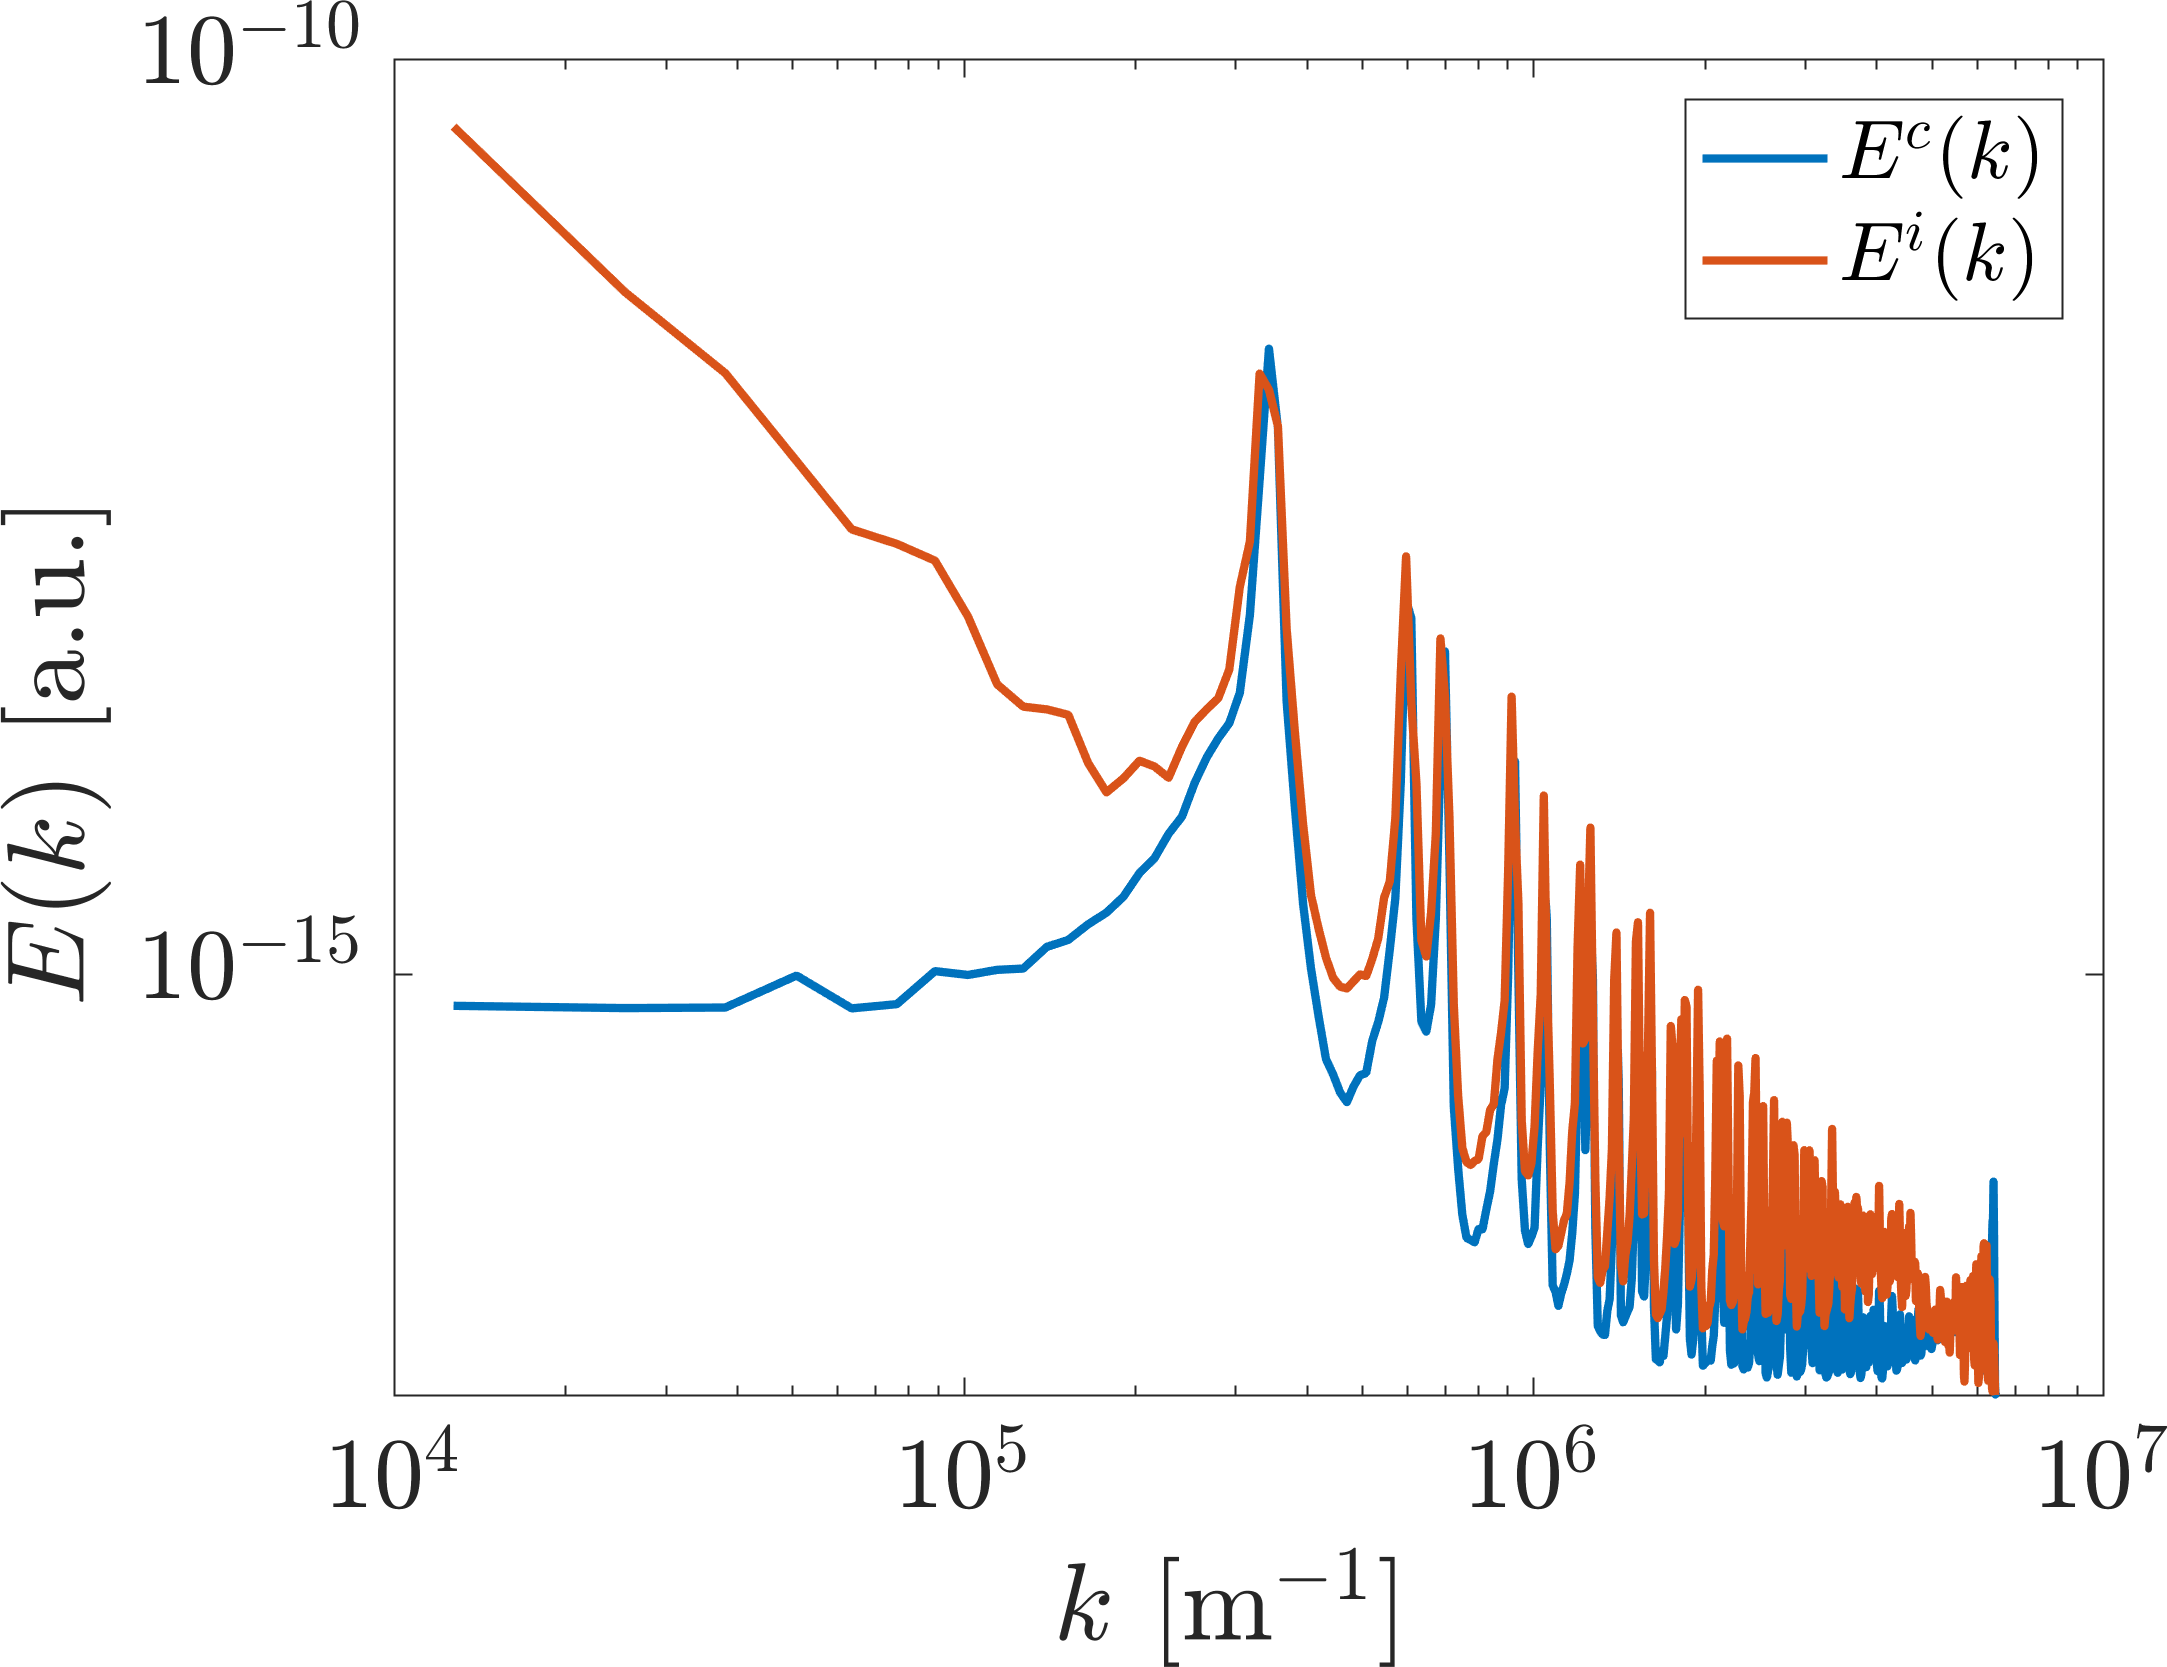
\includegraphics[width=0.45\textwidth,trim=0 0 0 0,clip=true]{ch5_kickit/Ek_classical/VTXLATT_Ek.png}
    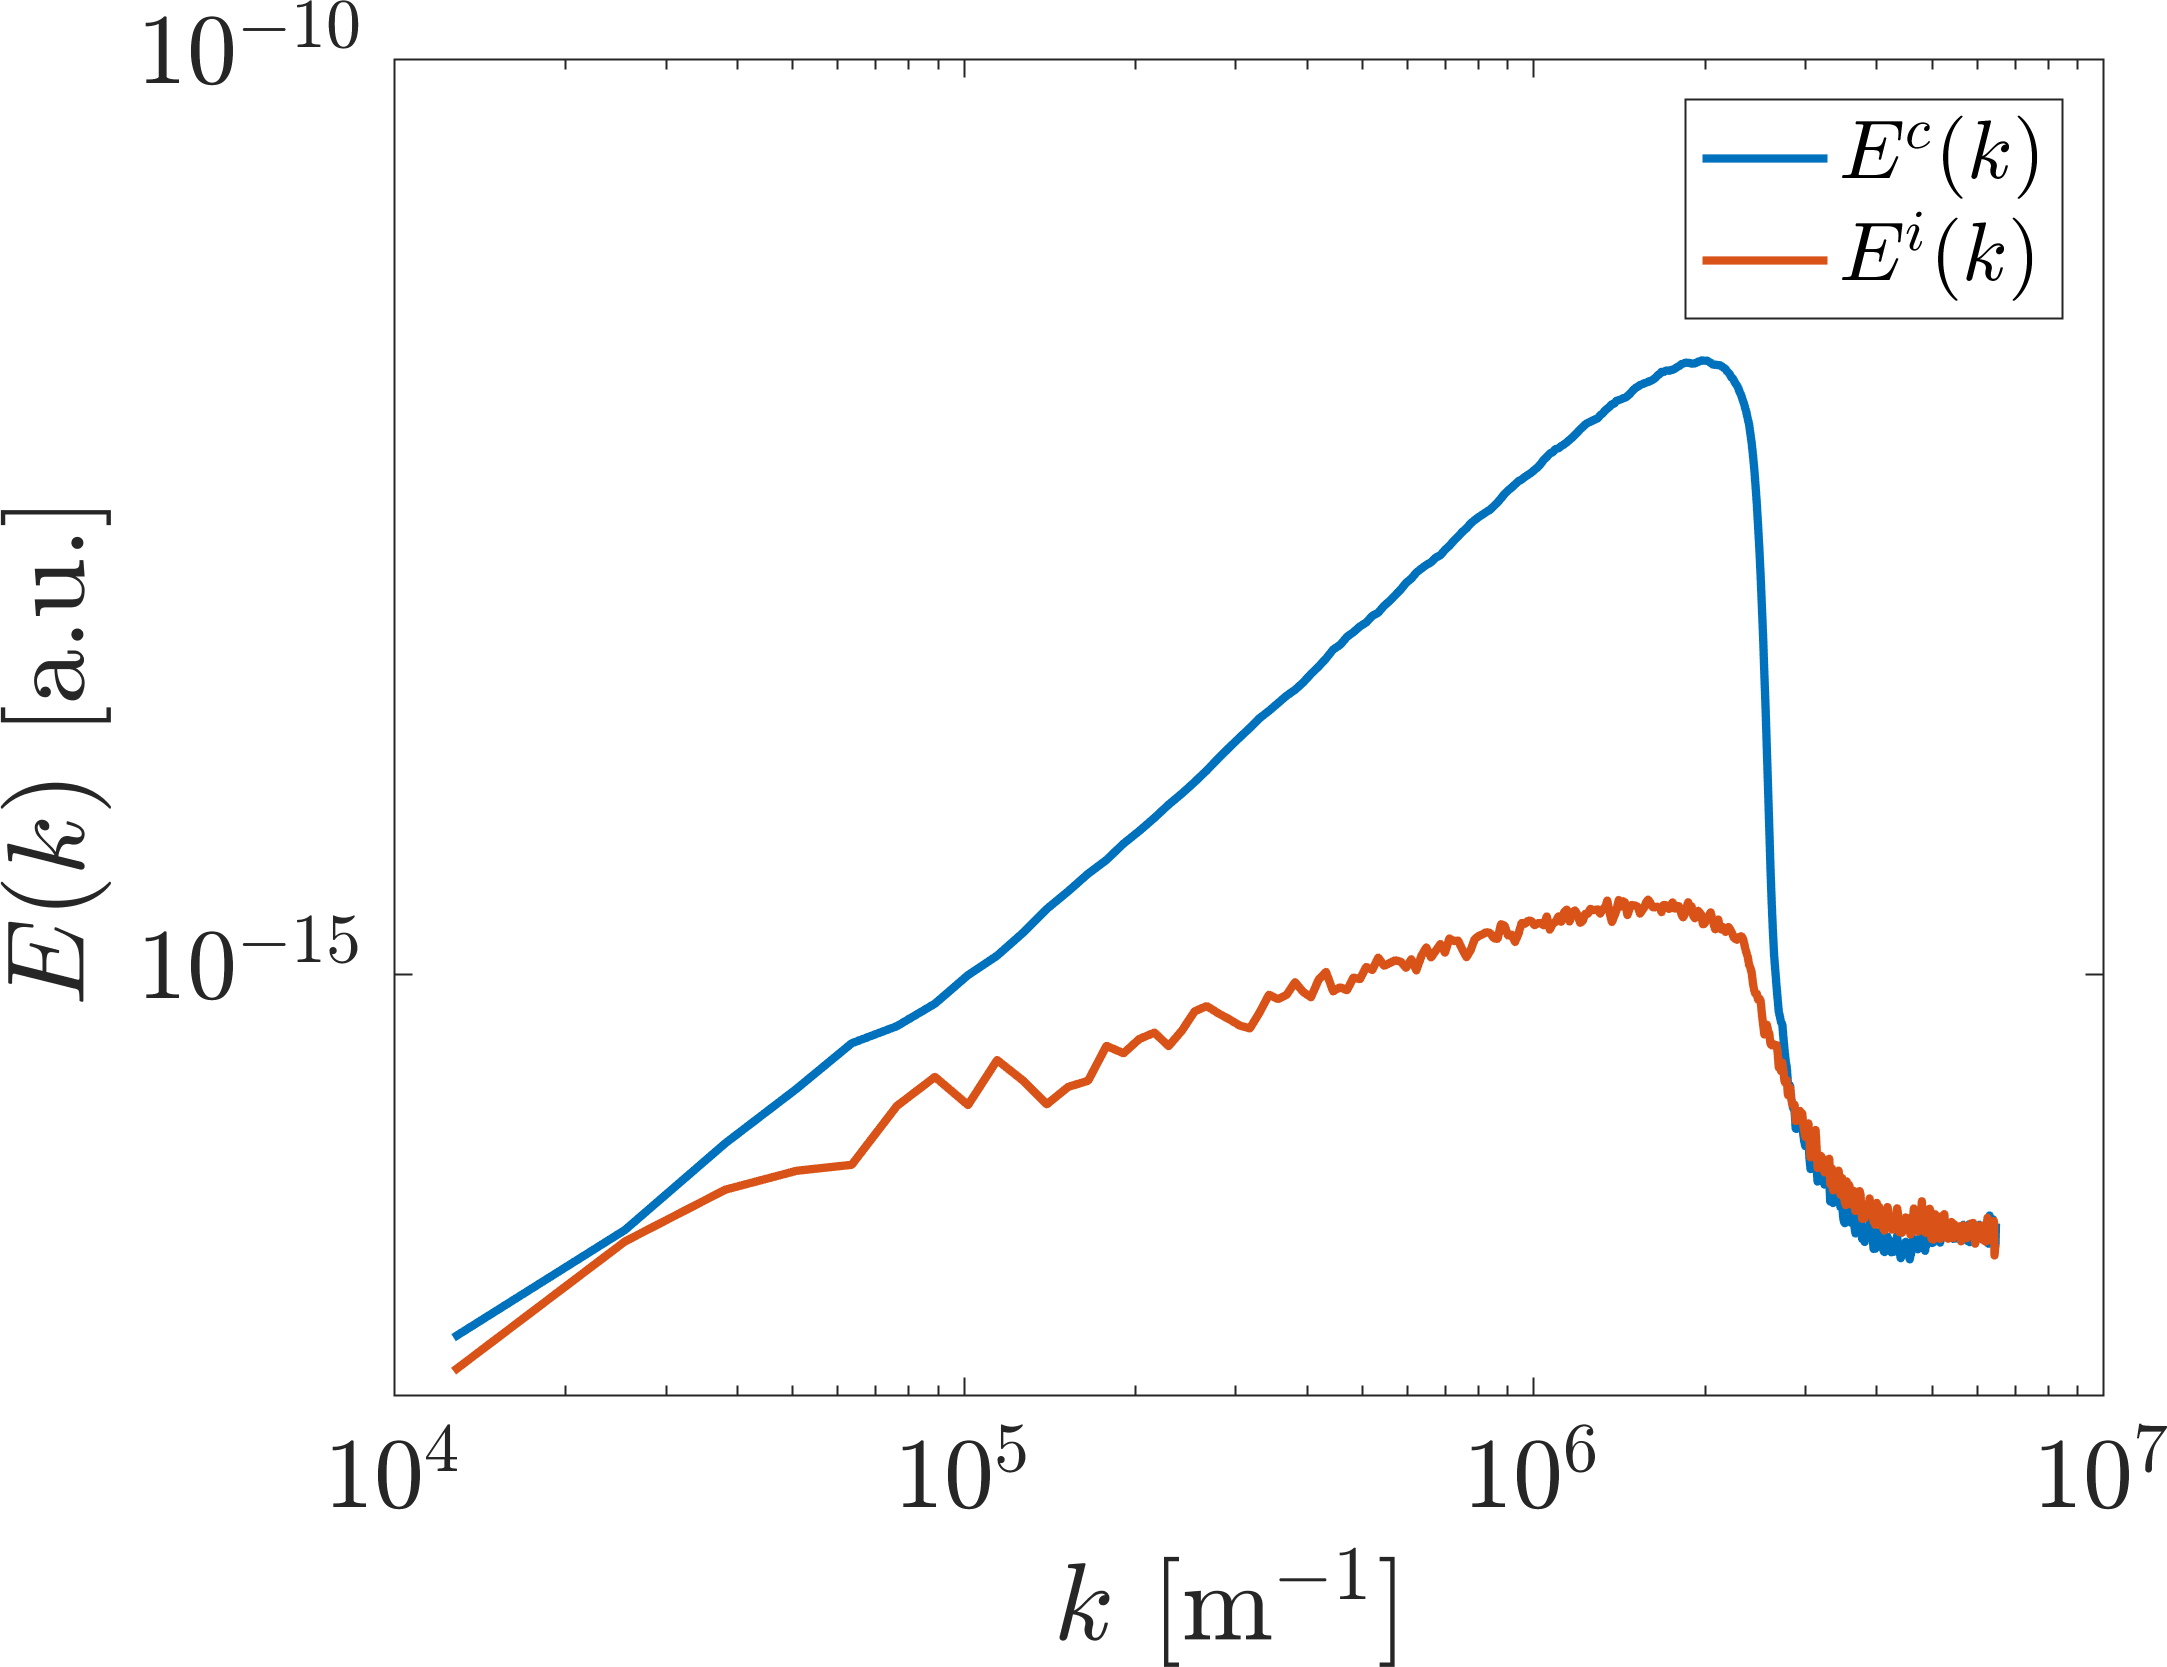
\includegraphics[width=0.45\textwidth,trim=0 0 0 0]{ch5_kickit/Ek_quantum/VTXLATT_Ek.png}
\iffalse
    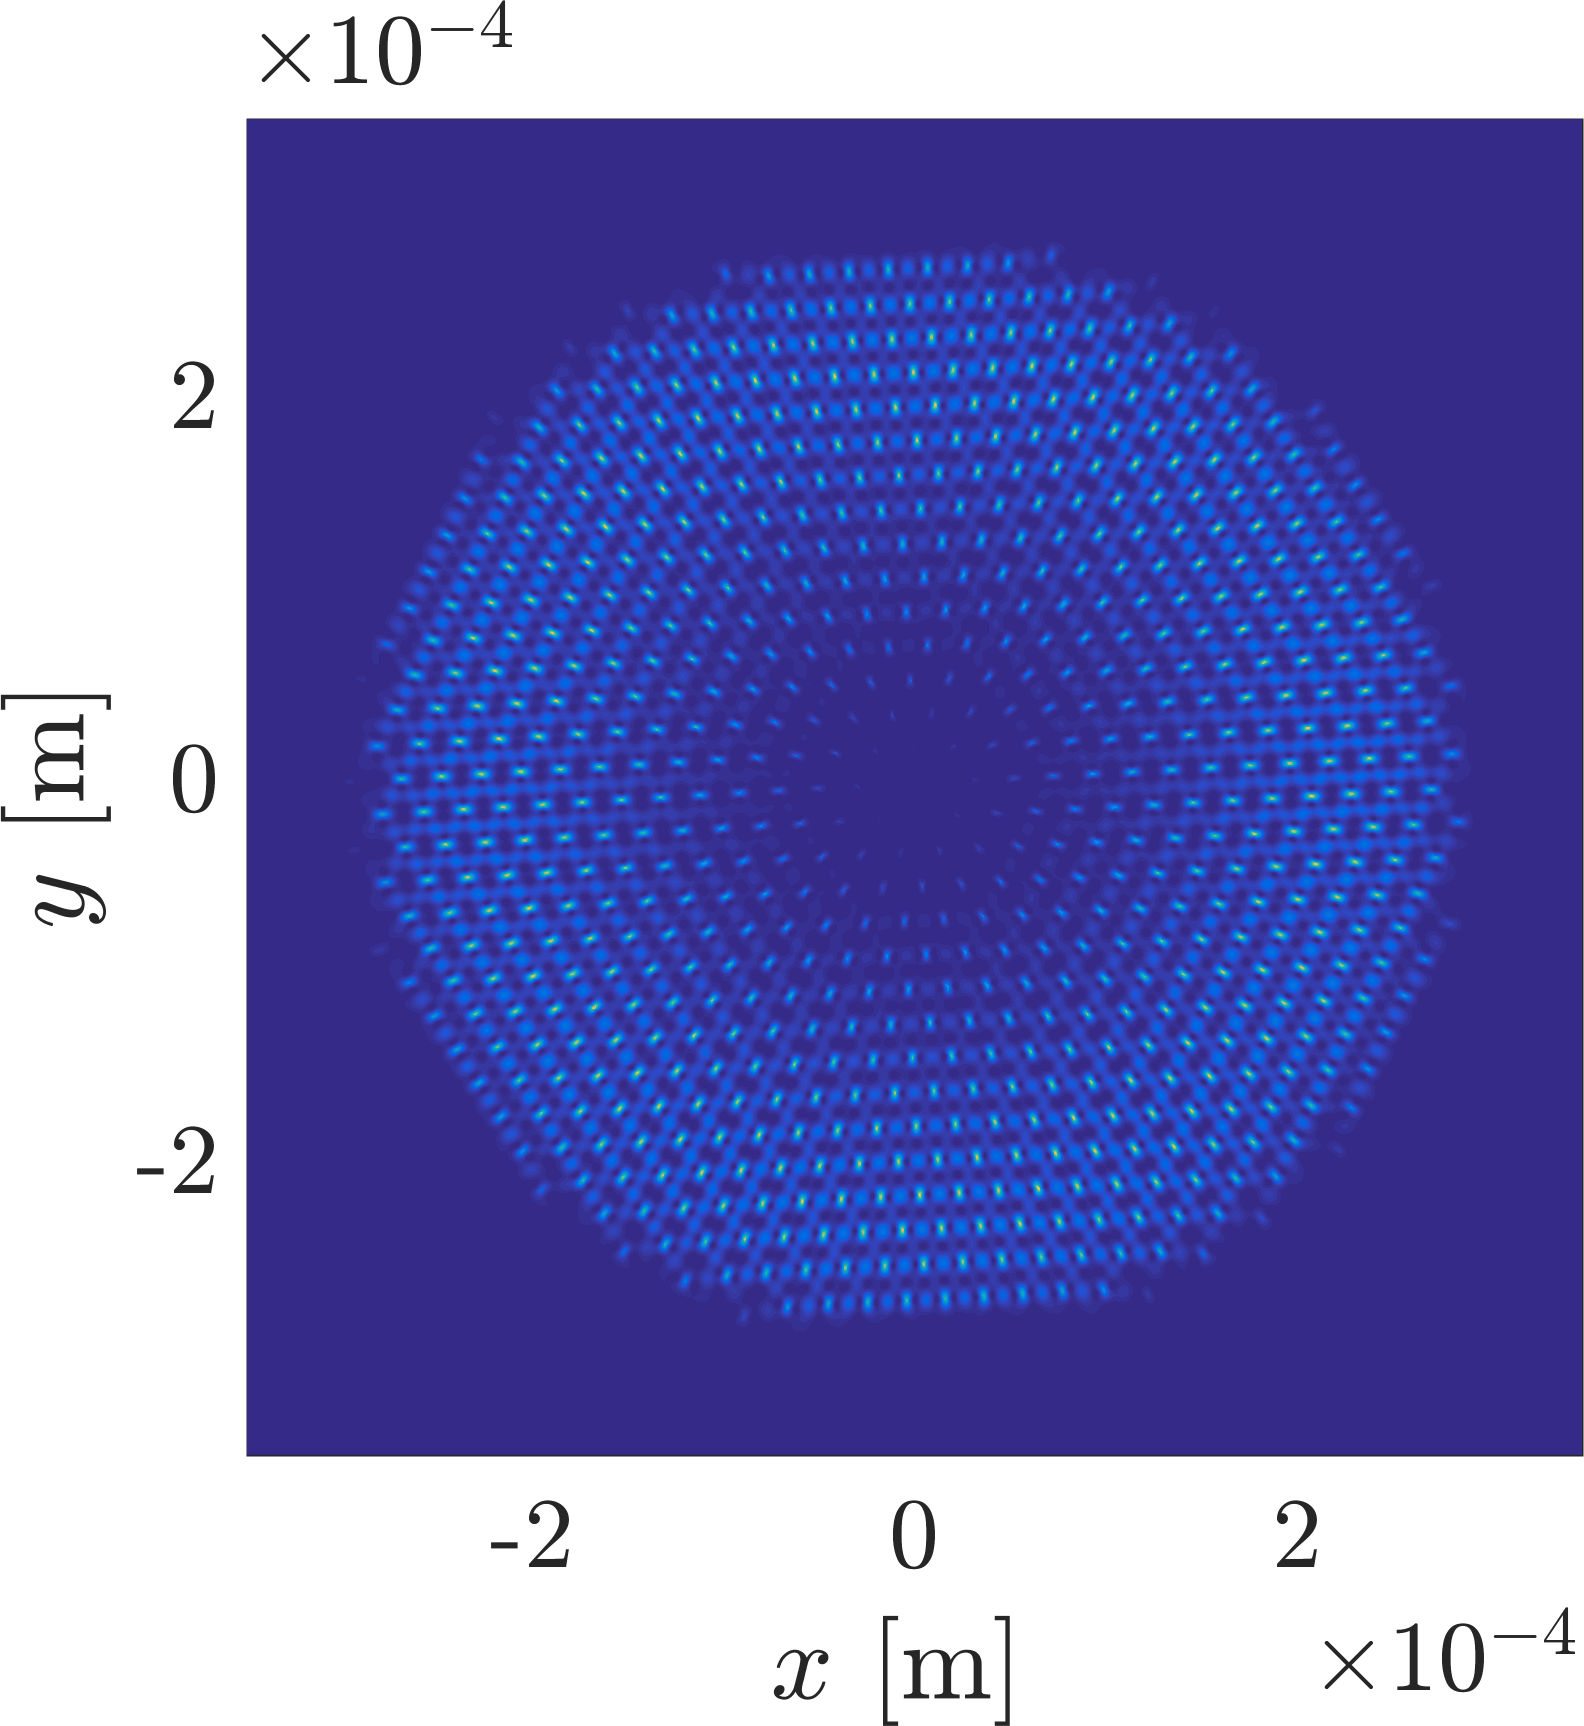
\includegraphics[width=0.45\textwidth,trim=0 0 0 0,clip=true]{ch5_kickit/Ek_classical/VTXLATT_Comp.png}
    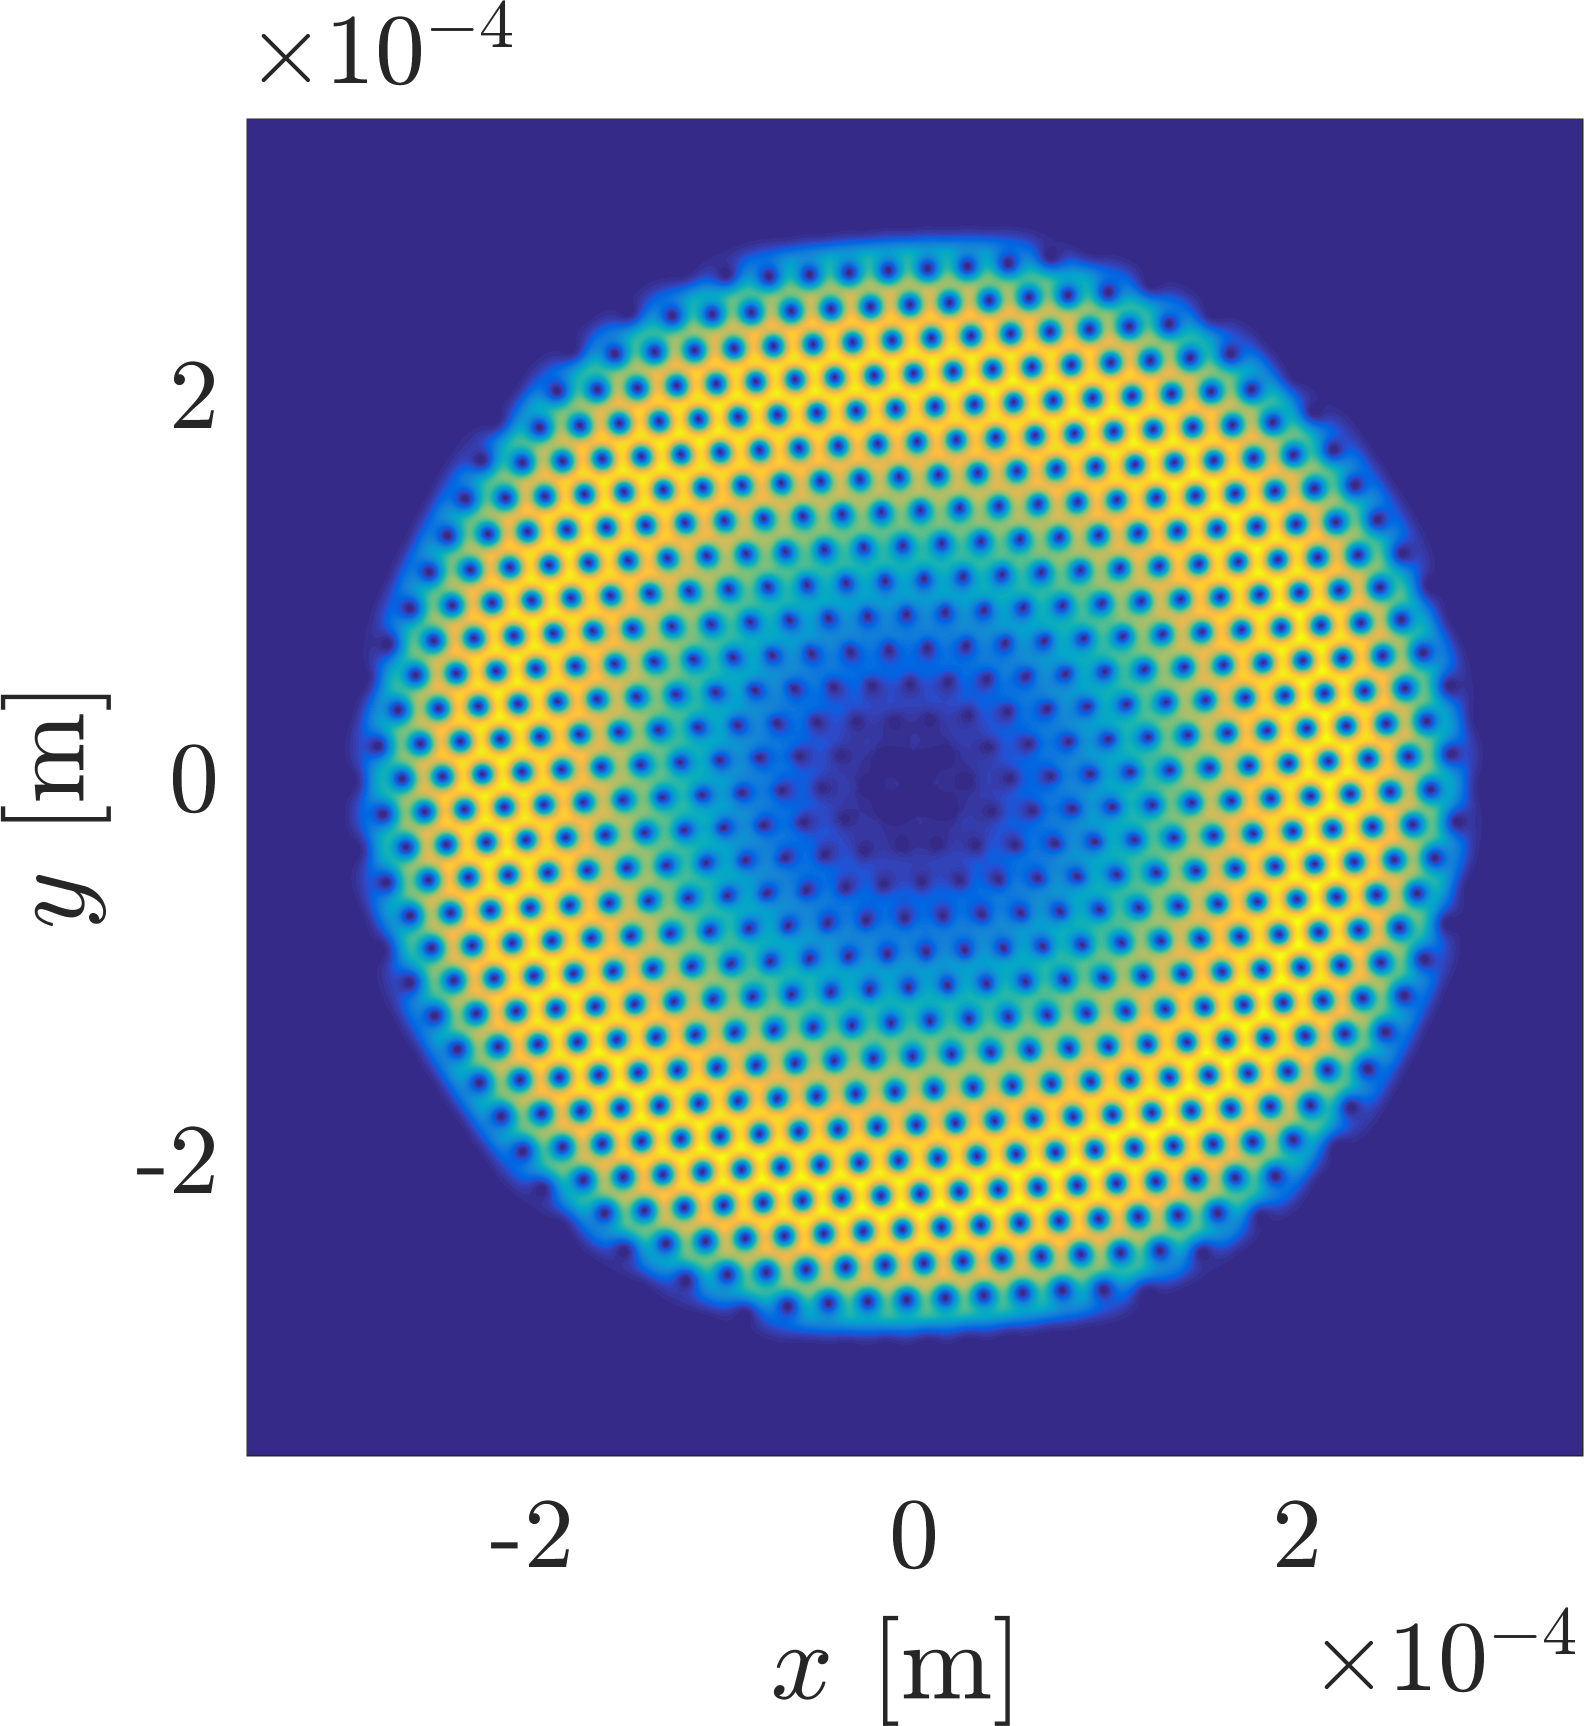
\includegraphics[width=0.45\textwidth,trim=0 0 0 0]{ch5_kickit/Ek_quantum/VTXLATT_Comp.png}

    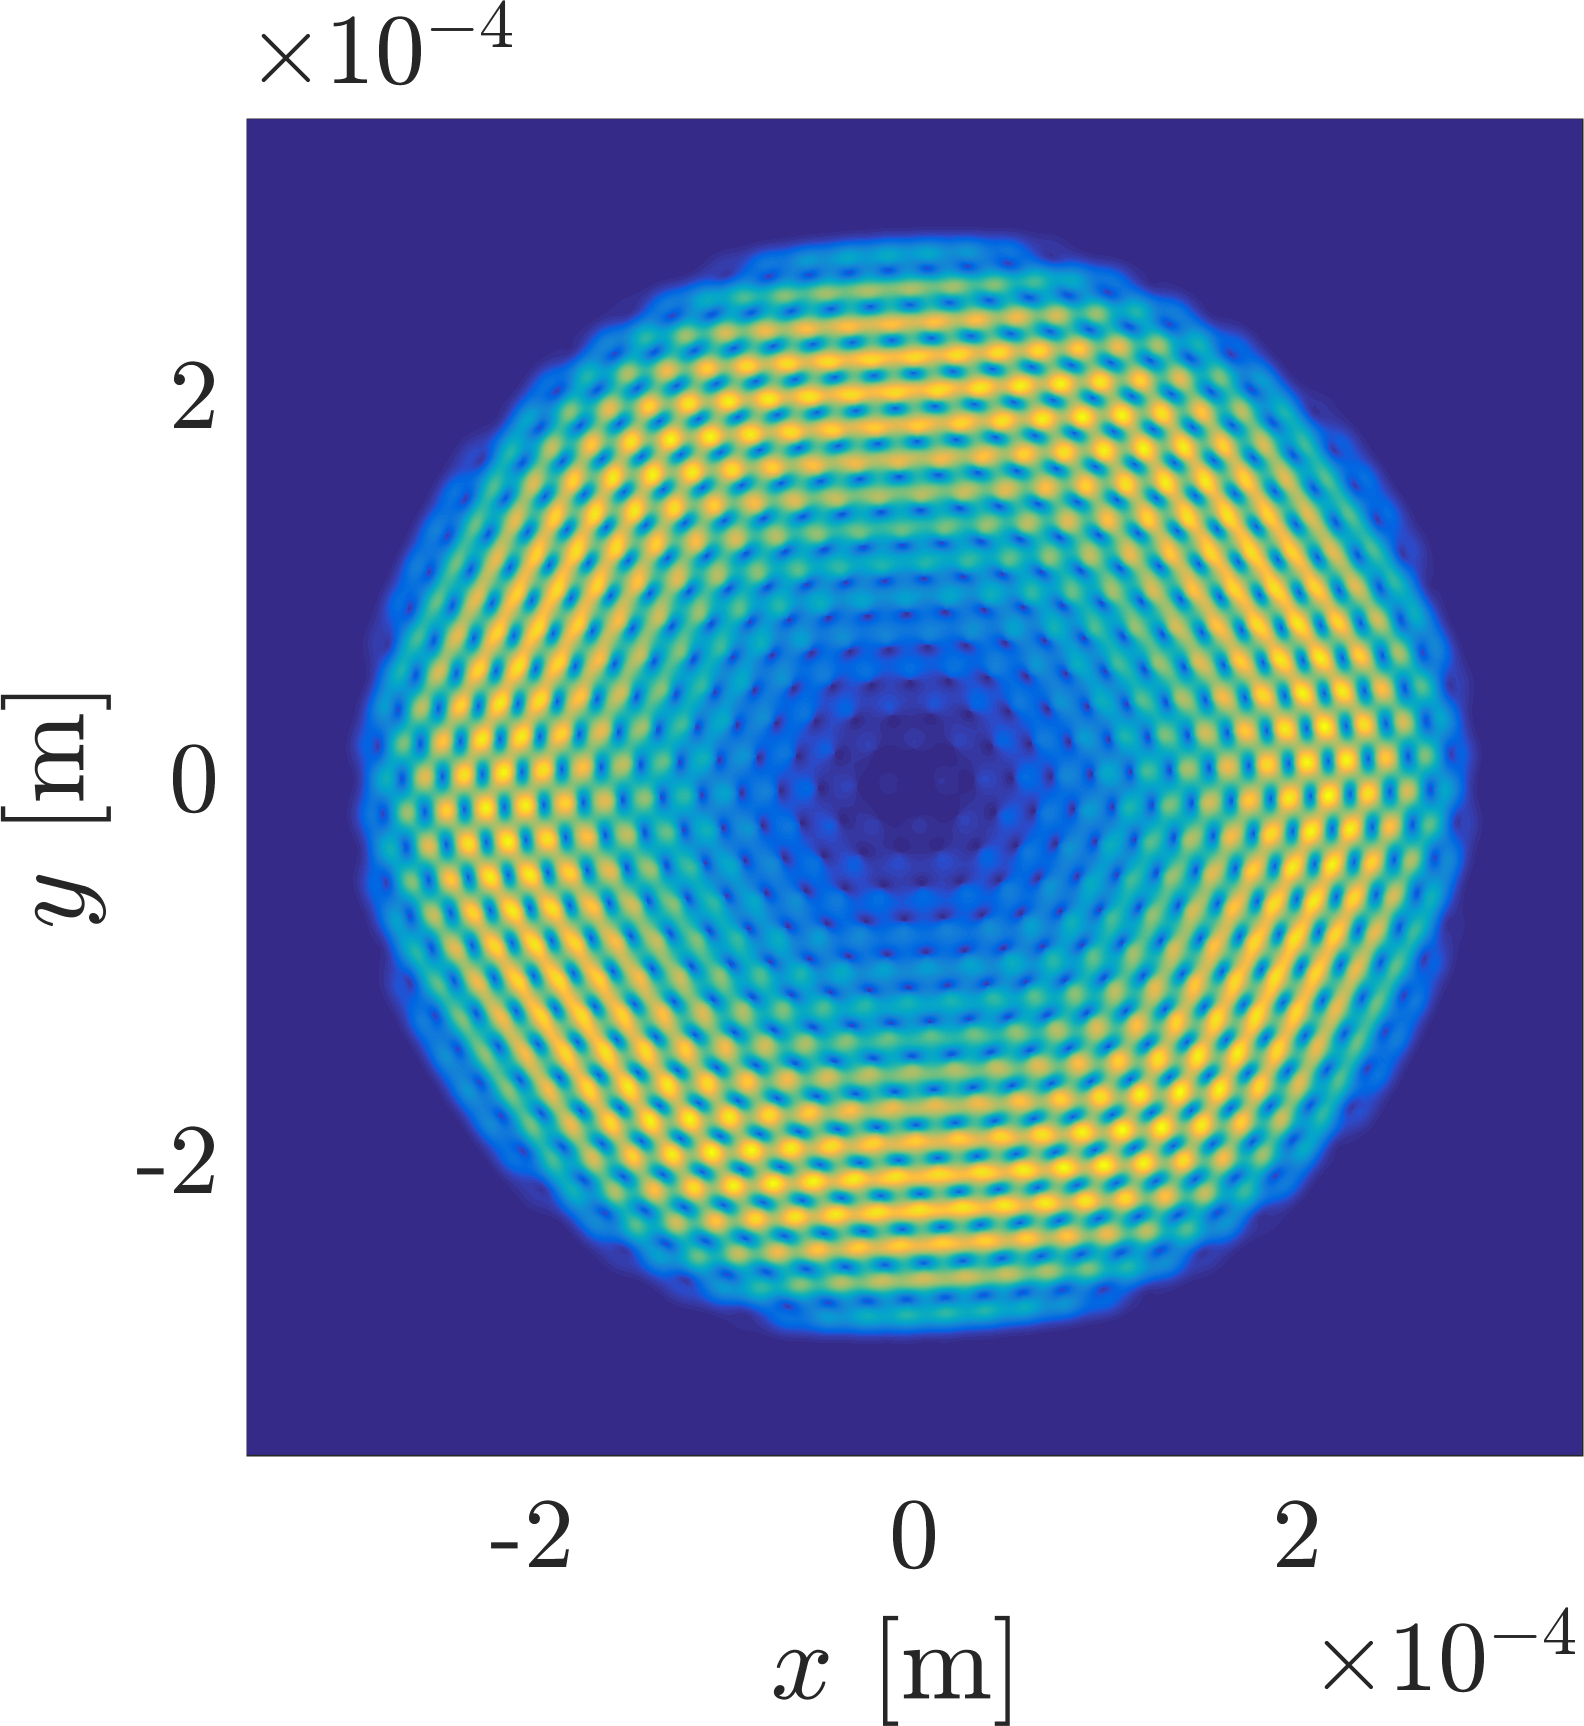
\includegraphics[width=0.45\textwidth,trim=0 0 0 0,clip=true]{ch5_kickit/Ek_classical/VTXLATT_Incomp.png}
    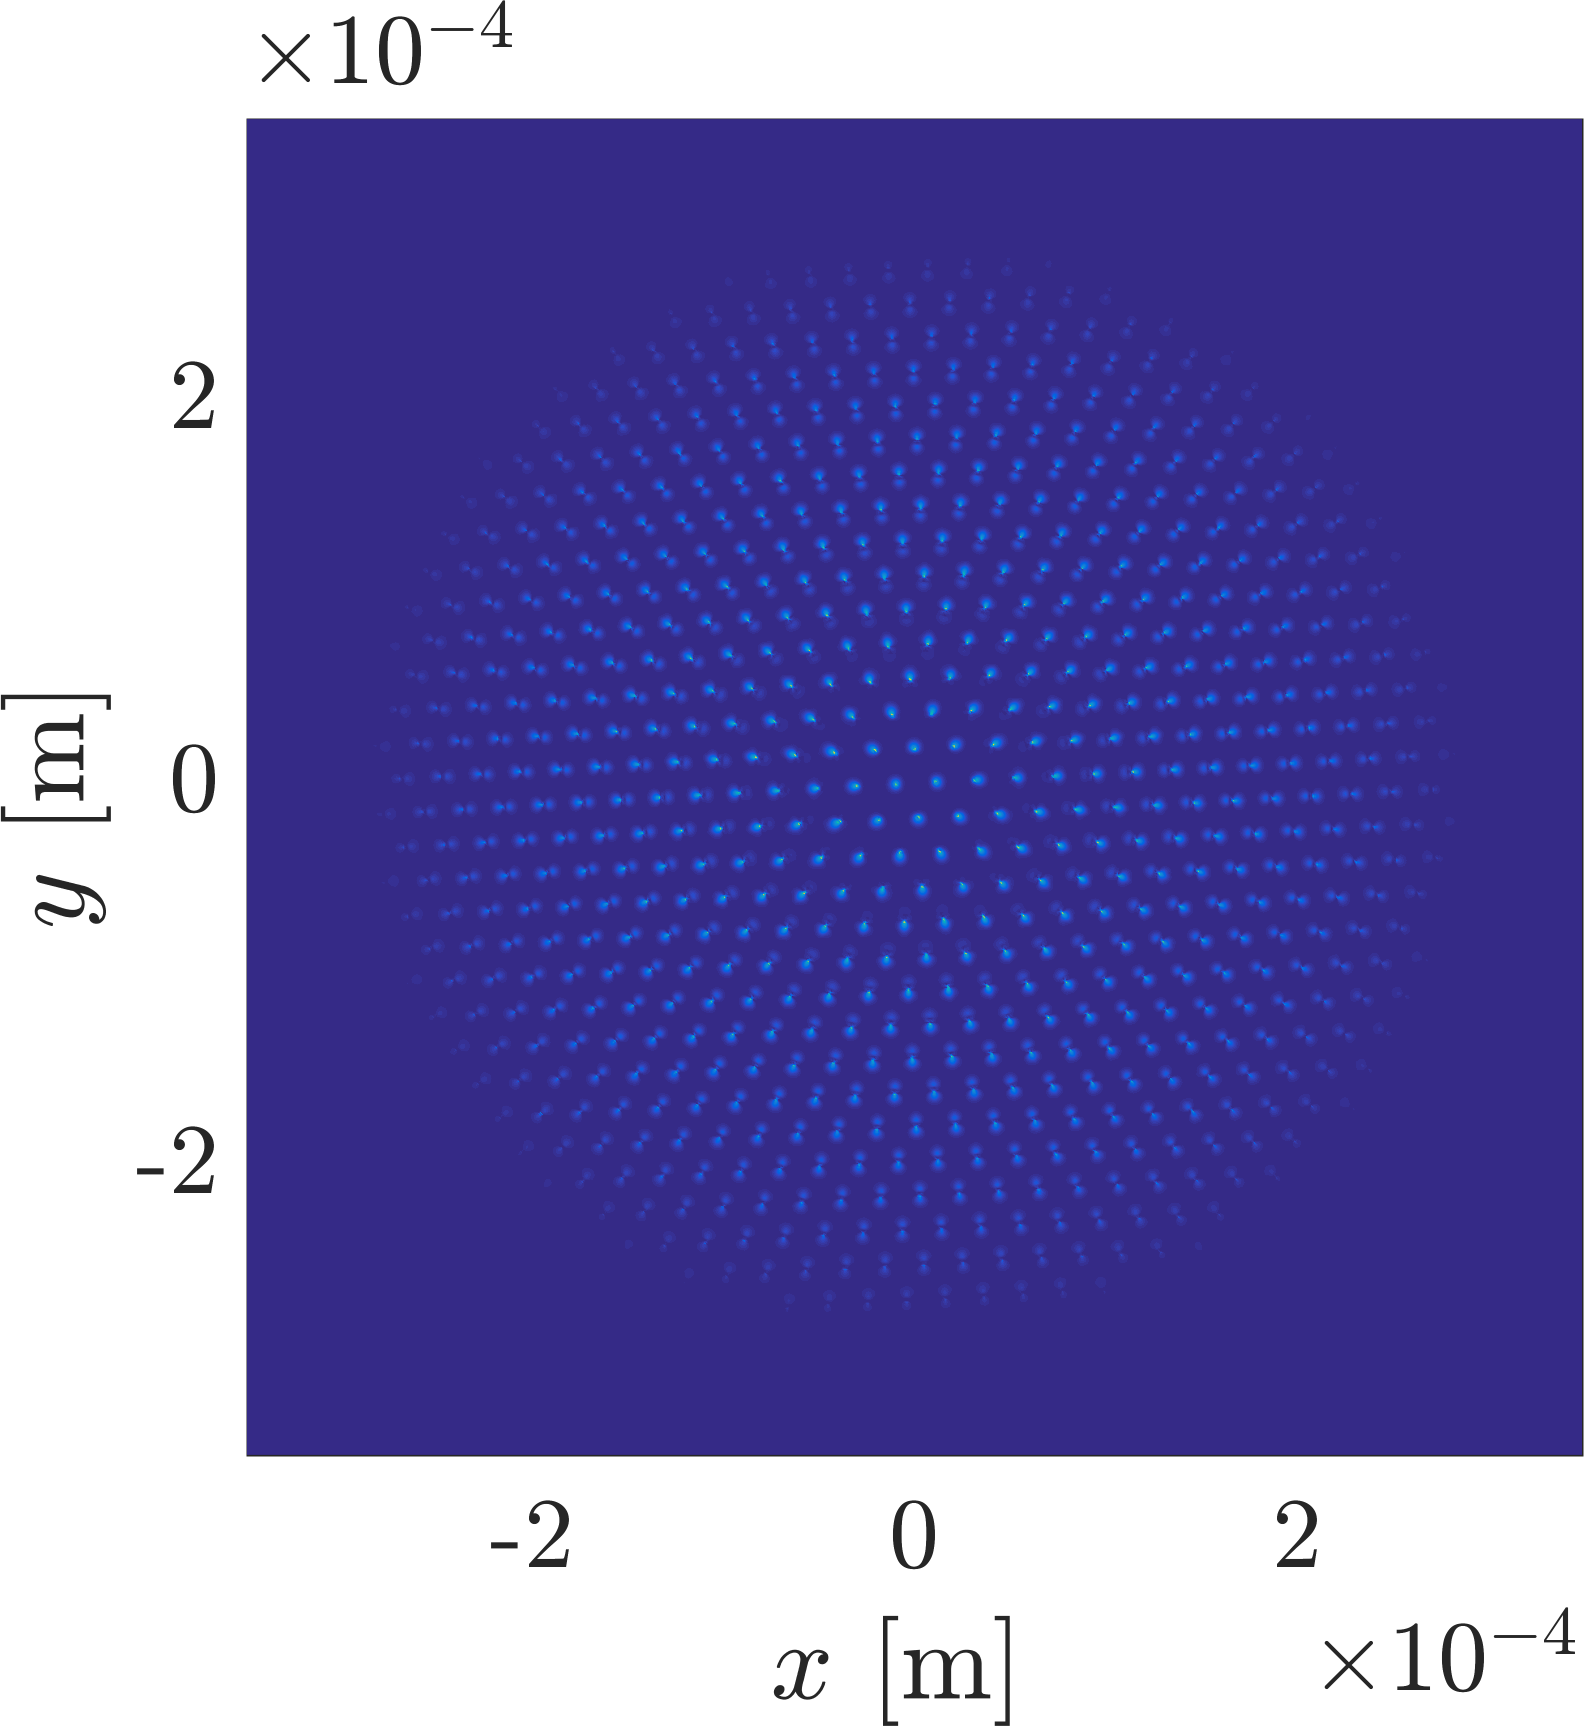
\includegraphics[width=0.45\textwidth,trim=0 0 0 0]{ch5_kickit/Ek_quantum/VTXLATT_Incomp.png}

    \caption[Kinetic energy spectra with and without quantum phase.]{The kinetic energy spectra (top row), compressible (middle row), and incompressible energies (bottom row), comparing the classical (left) and the quantum version (right). The inclusion of the phase term eliminates the peaks from the compressible energy, yet yields a more accurate representation of the magnitude of both energies (see text).}
\fi
\caption[Kinetic energy spectra with and without quantum phase.]{The kinetic energy spectra comparing the classical (left) and the quantum version (right).}
\label{fig:ek_clvqu}
\end{figure}


\section{Delta-kick dynamics}\label{sec:kickvl}
\subsection{Non-rotating condensate}
To fully characterise the effect kicking has on a rapidly rotating BEC carrying a vortex lattice it is instructive to first understand the dynamics following a kick in the absence of a vortex lattice. For an accurate comparison we need to take into account that in the absence of rotation no centrifugal forces appear, and we therefore adjust the trapping frequency of the non-rotating condensate such that the background densities match that of the rotating condensate. This is achieved from Eq.~\ref{eqn:vector_potential_gpe} by assuming the centrifugal term competing against the harmonic oscillator frequency  as $V_{\text{opt}} = 1/2m(\omega^2_\perp - \Omega^2)
{r}^2$, where $\Omega=0.995\omega_\perp$ is the value chosen for the rapidly rotating case, as given by Eq.~\eqref{eqn:vector_potential_gpe}.

For a stationary (non-kicked) condensate the kinetic energy spectrum will remain constant during time-evolution, with a kick leading to the appearance of new, time varying components. To observe this we numerically evolve the system by setting $V(\mathbf{r},t) = V_{\text{ext}}(\mathbf{r}) + V_{\text{opt}}(\mathbf{r},t)$, where the time dependent optical potential is only active for $\tau=10^{-5}$~s of the simulation time. As discussed earlier, this short kicking duration is sufficient to allow a phase imprint onto the condensate wavefunction, without any change in the density on the timescales of the kick itself. Next, we examine the compressible and incompressible kinetic energy spectrum following the kick (see Fig.~\ref{fig:ekc_eki_novtx}). Unsurprisingly, the spectrum is dominated by a peak corresponding to the wave-number associated with the optical potential at $k=4\pi/(\sqrt{3}a_o)$ (indicated by the dashed line), and several smaller ones corresponding to higher harmonics of $n$-th next nearest neighbour components of the lattice. This makes sense as the nearest neighbour lattice spacings should be the dominant structure with higher order spacings dropping in intensity due to the finite system size. As no rotation is added by the imparted phonon modes, the incompressible energy is an order of magnitude smaller compared to the compressible energy. Although the incompressible energy should technically be zero for a condensate with no vortices, given the difference in magnitudes this can be taken as a numerical issue, and can be assumed as zero. Following from this we will therefore restrict the analysis to the compressible part of the spectrum.

\begin{figure}
    %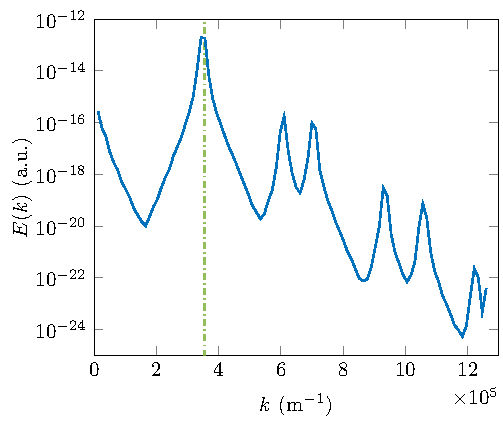
\includegraphics[width=0.48\textwidth]{ch5_kickit/fig2}
    \centering
    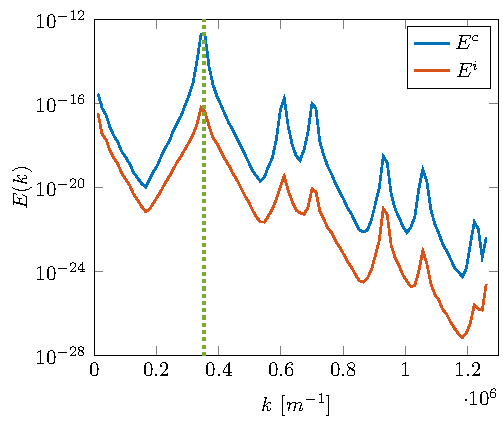
\includegraphics[width=0.55\textwidth]{ch5_kickit/EKcEKi_kick_dt2}
    \caption[Compressible and incompressible energy spectra of a non-rotating condensate directly following a kick.]{Compressible and incompressible energy spectra of a non-rotating condensate directly following a kick. A peak at $k=4\pi/(\sqrt{3}a_o)$ can be seen, which corresponds to the lattice spacing, $a_o$ (indicated by the dashed line), and the smaller, higher energy peaks can be attributed to higher harmonics between nearest and next-nearest neighbours. The incompressible spectrum is much smaller than the compressible spectrum, and thus is neglected for all further analysis.}
    \label{fig:ekc_eki_novtx}
\end{figure}


The evolution of the nearest neighbour peak in the compressible kinetic energy spectrum during the first 250 ms after the kick is shown in Fig.~\ref{fig:novtx_p5k}(a). It initially oscillates in and out of existence and eventually disperses over a wide range of wave-numbers. Snapshots of the density evolution are given in Fig.~\ref{fig:novtx_p5k}(b), which clearly show that the oscillations correspond to the existence of a transient lattice pattern with several revivals, having the same underlying structure as the optical potential. In fact, the lattice pattern is best formed whenever the main peak in the kinetic energy spectrum goes to zero, i.e.~when the imprinted kinetic energy has been converted into density modulations. The period of the oscillations can be related to the speed of sound given by
\begin{equation}
c(\textbf{r},t) = \sqrt{\frac{\rho (\textbf{r},t) g}{m}},
\end{equation}
divided by the lattice constant, and therefore the appearance of the lattice can be attributed to phonon interference.

\begin{figure}
    \centering

	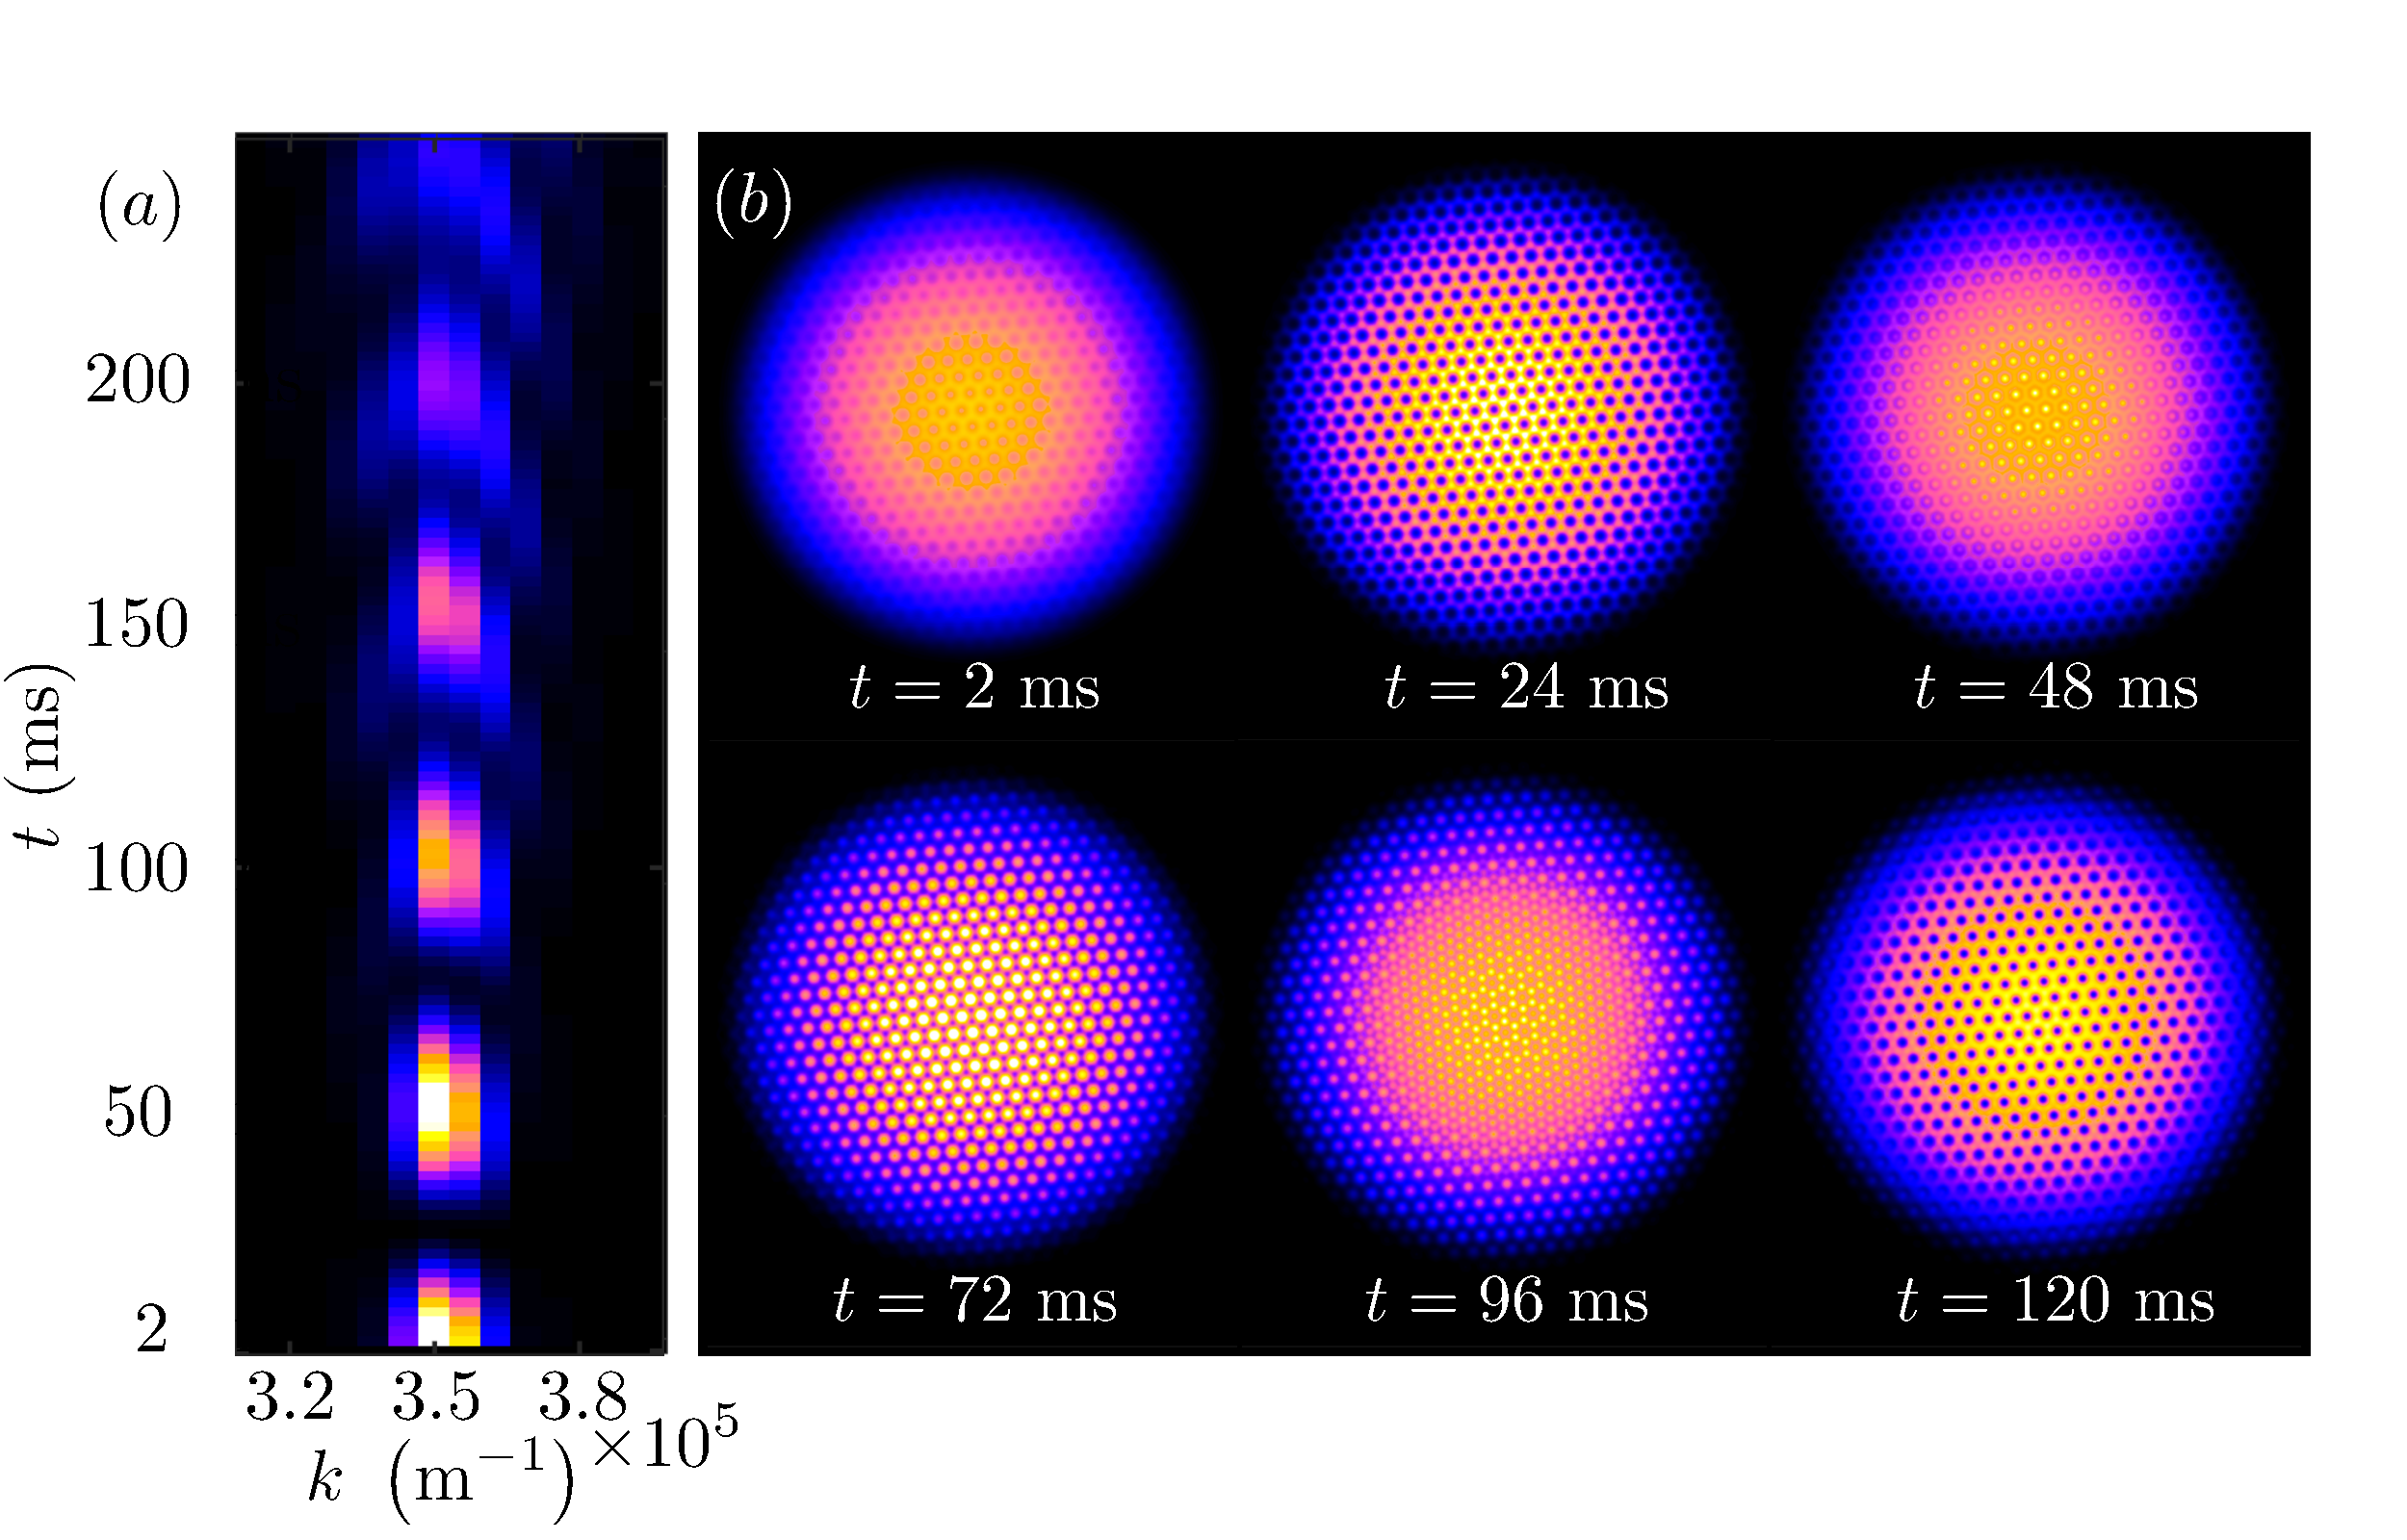
\includegraphics[width=0.80\textwidth]{ch5_kickit/fig3}
	\caption[Effect of kicking on non-rotating condensate.]{(a) Main peak of the compressible kinetic energy spectrum for a kicking strength of $V_0 \approx 1.35\times10^{-2}\mu$. It can be seen to revive, and eventually disperse over a wide range of wave-numbers.  (b) Condensate densities at several times during the evolution. A pattern matching the optical potential can be observed to appear and disappear several times over the course of the evolution.}
	\label{fig:novtx_p5k}
\end{figure}


%######################################################%#################################################################################%############################################################################################################
\subsection{Rapidly rotating condensate}

    Kicking a condensate carrying an Abrikosov vortex lattice with the above optical lattice gives an additional parameter, $\theta_\Delta$, which describes the orientation of the imprinted phonon lattice angle relative to the vortex lattice. For simplicity, it is assumed that the vortex and optical potential lattices have the same lattice constant, $a_v=a_o=a$ (see below for a discussion of the incommensurate case), which means that symmetry allows for a restriction of the angle to $\theta_\Delta\in[0,\pi/3]$. In the following it can be seen that adjusting $\theta_\Delta$ leads to the appearance of different, transient super-structures in the condensate density.

    If $\theta_\Delta=0$ (see Fig.~\ref{fig:moire_density}(a)) the kicking imparts kinetic energy at wave-numbers that are already well defined in the lattice. No significant change to the compressible kinetic energy spectrum is observed in this case, apart from small amplitude modulations on the well defined peaks.

	\begin{figure}
        \centering
			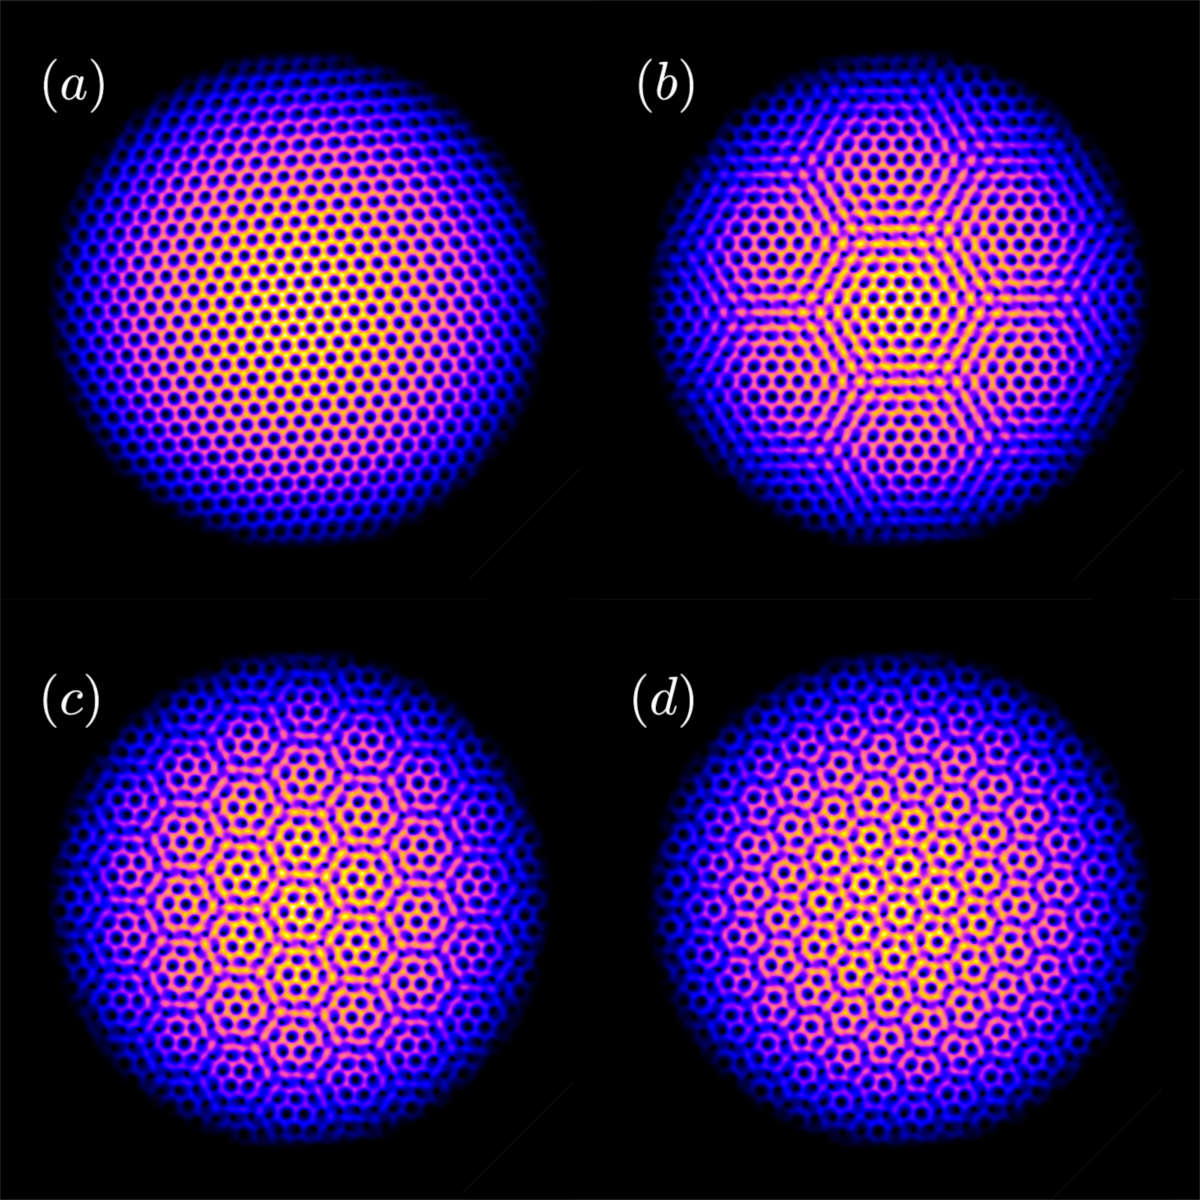
\includegraphics[width=0.55\textwidth]{ch5_kickit/fig4}
			\caption[Effect of kicking on condensate with a large vortex lattice.]{Condensate density at $t=1.4\times10^{-2}$ s for several optical lattice rotation angles. The cell size of the super-lattice structures can be seen to shrink as the angle is increased. The angles for the examples shown are $(a)~\theta_\Delta=0$, $(b)~\theta_\Delta=2\pi/45$, $(c)~\theta_\Delta=4\pi/45$, $(d)~\theta_\Delta=2\pi/15$. }
			\label{fig:moire_density}
		\end{figure}

    However, if the angle between both lattices is finite, and not an integer multiple of $\pi/3$, superlattice structures appear after a short time (see Fig.~\ref{fig:moire_density}(b)-(d)), which have a structure cell size that decreases for increasing values of $\theta_\Delta\in[0,\pi/6]$ and beyond which increases for larger values until the misalignment angle reaches the lattice symmetry point again at $\theta_\Delta=\pi/3$. These structures are transient, and several revivals can be observed before the condensate settles back into the vortex lattice structure with an increase in the background wave-number spread, as expected based on kicking the non-rotating condensate. An example of this for a fixed angle is shown in Fig.~\ref{fig:dtheta20_ev}.

	\begin{figure}
        \centering
		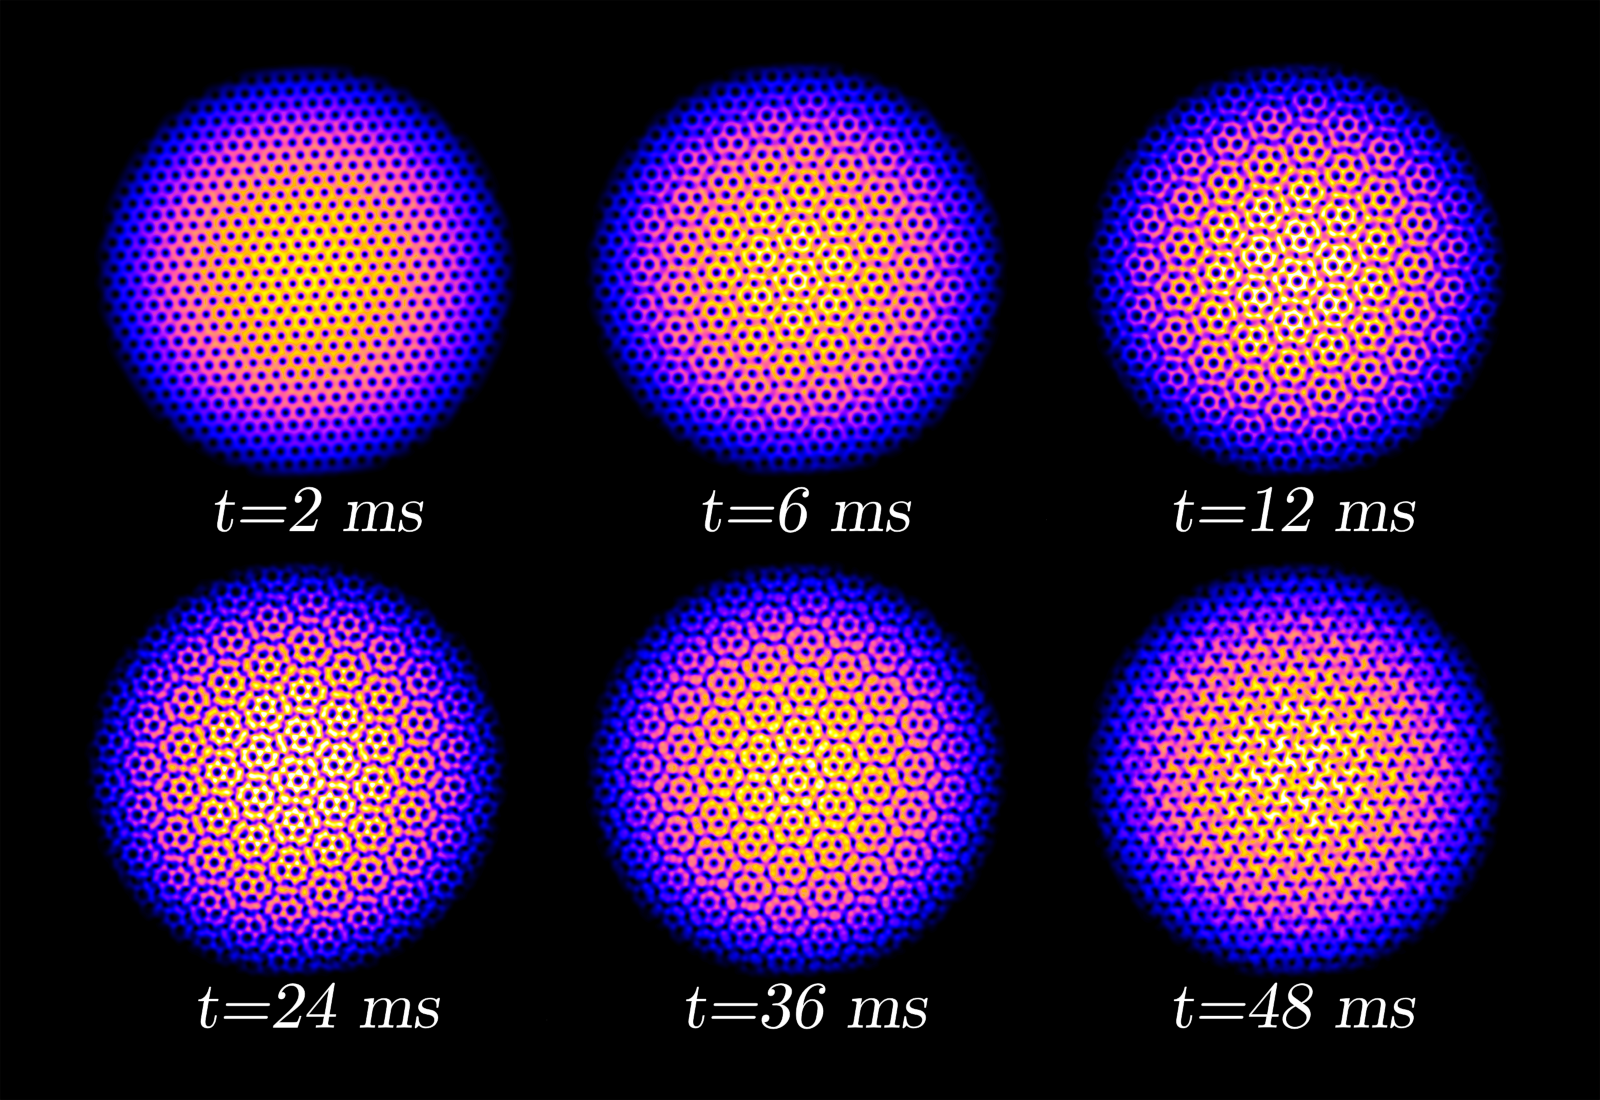
\includegraphics[width=0.55\textwidth]{ch5_kickit/fig5}
		\caption[Oscillation of moir\'e wavelength.]{Condensate density shows visible moir\'e structures upon receiving a kick with $\theta_\Delta=\pi/9$. The appearance and disappearance of a moir\'e structure with wavelength $\lambda_M \approx 2.9 a$ over a timescale of about $50$ ms can be seen.}
		\label{fig:dtheta20_ev}
	\end{figure}

    To explain the interference patterns observed for misaligning the optical and the vortex lattice, we employ moir\'e interference theory \cite{SS:Hermann_jpcm_2012}. Moir\'e patterns are known to appear when two periodic structures are overlaid while slightly misaligned to each other, and can be calculated from the reciprocal lattice vectors. In all generality, any choice of equidistantly separated reciprocal lattice vectors can be parameterised as
    	\begin{equation}
    		\mathbf{g}_{l} = g_0 \left[ \sin\left( \frac{2\pi l}{\upsilon}+\theta \right),\, \cos\left( \frac{2\pi l}{\upsilon} +\theta\right) \right],
    	\end{equation}
    where $\upsilon$ describes the rotational symmetry of the lattice, $l$ labels the vector direction on the unit circle, $\theta$ is the angle with respect to a chosen coordinate system and $g_0$ is the reciprocal lattice constant. For commensurate and triangular lattices we get $g_0=4\pi/(\sqrt{3}a)$, $\upsilon=6$ and the vector directions are $l=\left[0\dots\upsilon-1\right]$. As only the relative mis-alignement between the vortex and the phonon lattice matters, we choose $\theta=0$ for the vortex lattice and $\theta=\theta_\Delta$ for the optical potential alignment.
    All possible wavelengths that can appear in an interference pattern between two such lattices in position space are then given by
    	\begin{equation}
    		\lambda_{ll'} = \frac{\lambda_0}{|\mathbf{\mathbf{g}_{ll'}|}},
    		\label{eq:InterferenceVectors}
    	\end{equation}
    where
    $\mathbf{g}_{ll'}=\mathbf{g}_{l}^{\text{V}}-\mathbf{g}_{l'}^{\text{P}}$, and
    $\lambda_0 = 4\pi/\sqrt{3}$ for the commensurate triangular lattices. This yields 6 interfering wavevectors, and as a result 6 moir\'e wavelengths. Figure~\ref{fig:moire_higher} shows these resulting interferences in both position and reciprocal space, with colour indicating the corresponding wavenumber-wavelength. The band-like structure of the interferences have contact points at the angle of maximal and minimal alignment of the two lattices, $\theta_\Delta=(j\pi/3,j\pi/3)$ respectively. For a chosen rotation angle between these limiting values, we obtain several wavenumbers, and hence wavelengths. One can see from Fig.~\ref{fig:dtheta20_ev} for $\theta_\Delta = \pi/9$ that a pattern matching the longest wavelength, $\lambda_M= \max[\lambda_{ll'}] \approx 2.9 a$, appears around $t=24$~ms and is clearly the most visible one for the given angle. Shorter wavelengths, while are expected to be present, are hard to discern in this system, and therefore we will concentrate on the lowest wavenumber for the following analysis.

In $\mathbf{k}$-space the shortest $|\mathbf{g}_{ll^\prime}|$ corresponds to adjacent wave-vectors with the smallest $\theta_\Delta$ between them (see inset in Fig.~\ref{fig:moire_lambda_1}). Due to the symmetry of the lattices the most visible structures are therefore given by $\lambda_M=\lambda_{00}$ for $\theta_\Delta\in[0,\pi/6]$ and $\lambda_M=\lambda_{01}$ for $\theta_\Delta\in[\pi/6,\pi/3]$ (see inset of Fig.~\ref{fig:moire_lambda_1}).
While this symmetry assumption no longer holds strictly true after the system has been kicked, it is still fulfilled to a very good approximation during the initial dynamics. One can then obtain the wavelength of the dominating moir\'e structure as~\cite{BIO:Blair_jneur_2007,SS:Yankowitz_natphys_2012}
    	\begin{equation}
    		\lambda_M = \frac{a}{2\sin(\eta/2)},
    		\label{eqn:moire_size}
    	\end{equation}
    where $\eta=\min\{\theta_\Delta,\frac{\pi}{3} - \theta_\Delta \} $  (see Fig.~\ref{fig:moire_lambda_1}).
These super-structures become observable when the wavelength becomes smaller than the radius of the condensate, which for the chosen parameters is $\lambda_M \approx 11a$ and which corresponds to an angle $\theta_\Delta \approx \pi/36$.
One can see from Fig.~\ref{fig:moire_lambda_1} that once the relative angle is increased beyond this value the structure sizes shrink to a minimum value at the point of complete misalignment, $\theta_\Delta=\pi/6$, giving $\lambda_M\approx 1.93\,a$, and increase again up to the point of symmetry. Beyond this point the behaviour starts over, due to the symmetry of the lattice. Note that in principle the above procedure can be carried out for square or other optical lattice geometries.

\begin{figure}
    \centering
    %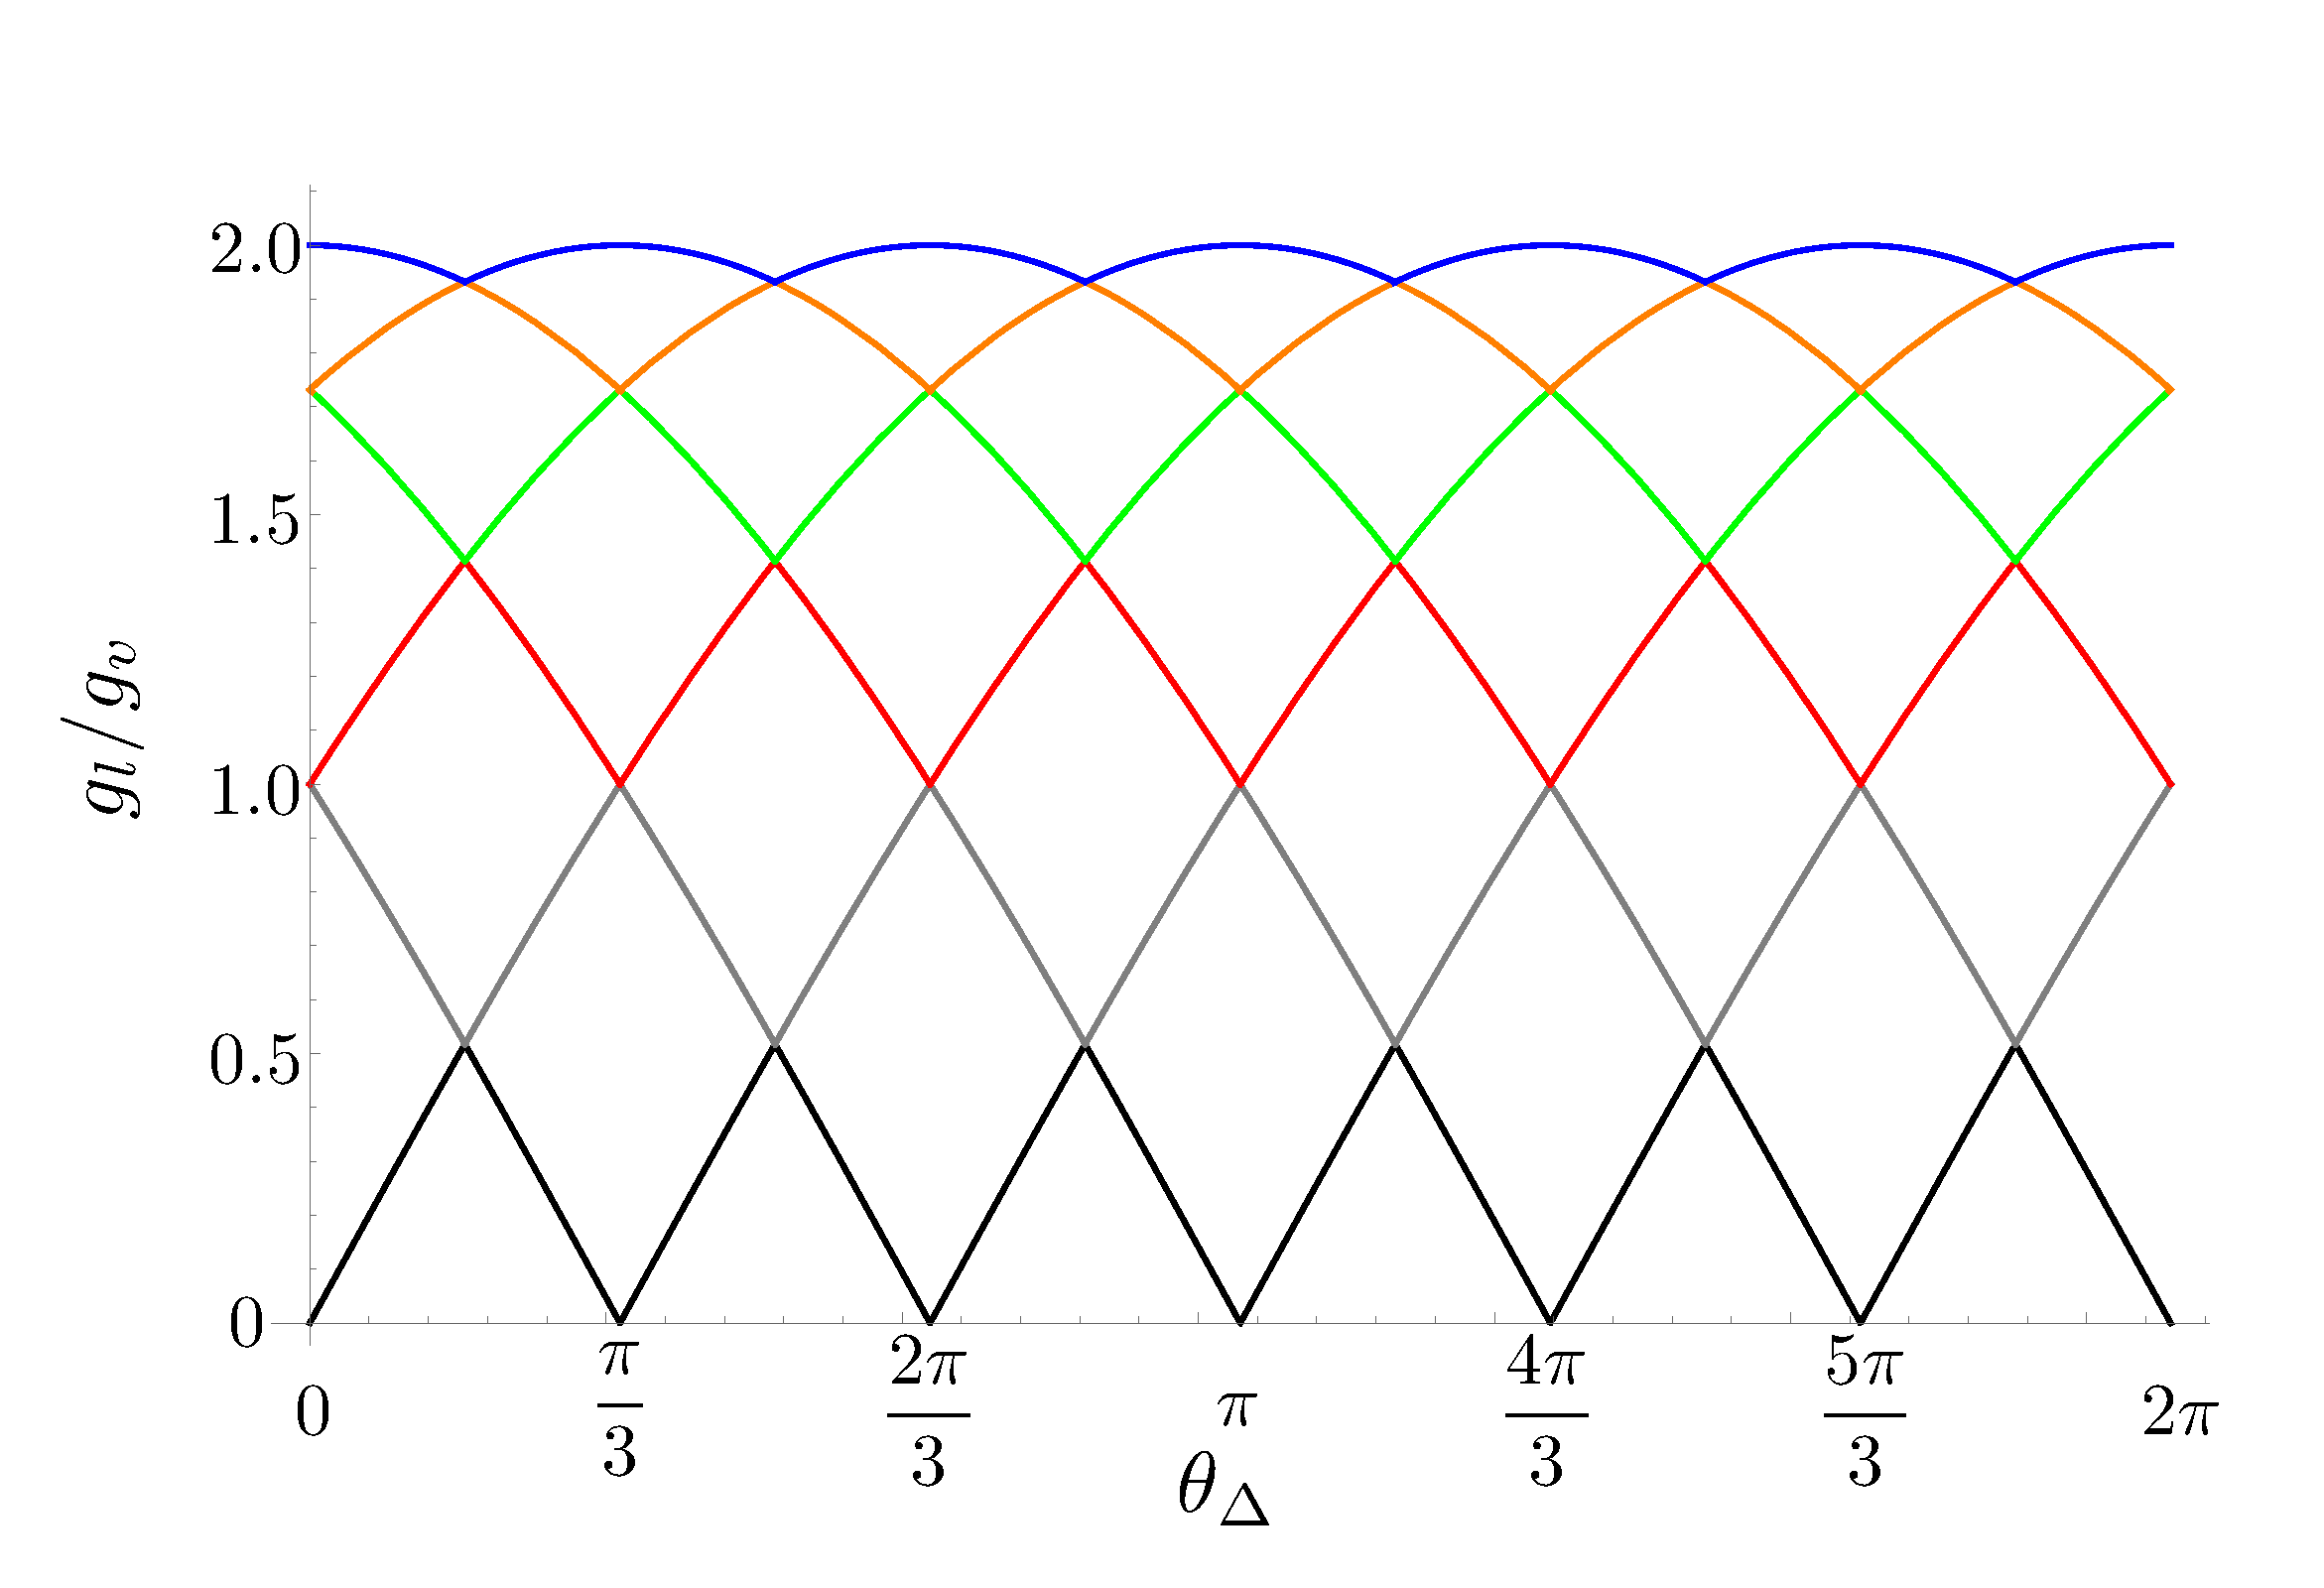
\includegraphics[width=0.48\textwidth,page=1]{ch5_kickit/Moire_lattice_BEC_HigherK_lambda}
    %\includegraphics[width=0.48\textwidth,page=2]{ch5_kickit/Moire_lattice_BEC_HigherK_lambda}
    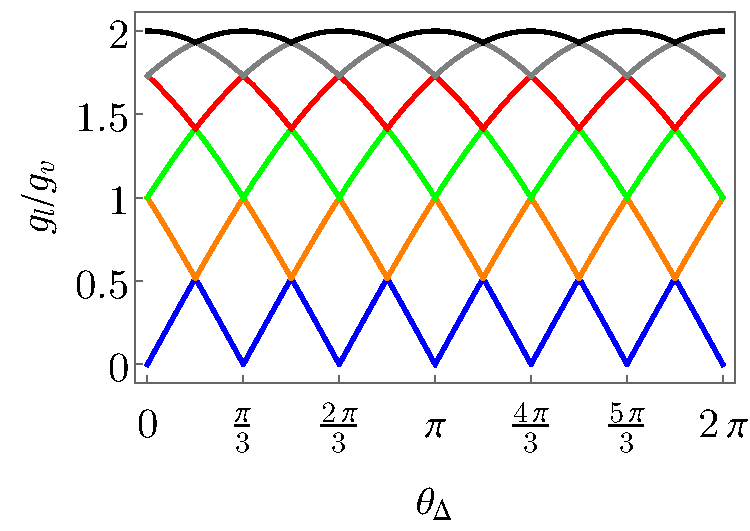
\includegraphics[width=0.48\textwidth]{ch5_kickit/HigherK_k}
    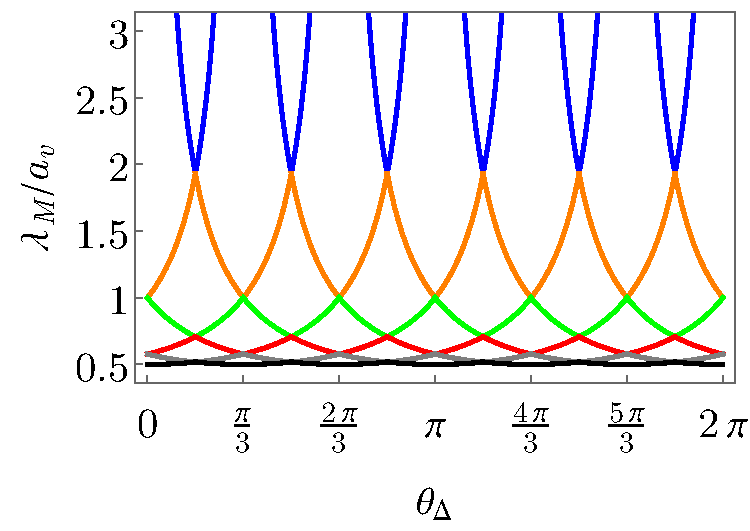
\includegraphics[width=0.48\textwidth]{ch5_kickit/HigherK_lambda}
    \caption[The moir\'e interference pattern in terms of wavenumbers.]{The moir\'e interference pattern in terms of wavenumbers (left) and corresponding wavelengths (right). The resulting wavenumber $g_l$ is normalised by the vortex lattice spacing in reciprocal space $g_v$, and the moir\'e wavelength $\lambda_M$ is normalised by the vortex spacing in position space $a_v$. The lowest lying band in reciprocal space is the main contributor to the visible moir\'e interference patterns, corresponding to the largest wavelength (both in blue). Higher orders are shown for the reciprocal and the corresponding position space, with the higher modes only visible between the beats of the lowest wave-number moir\'e interferences. Colours correspond between wavelengths and wavenumbers.}\label{fig:moire_higher}
\end{figure}

\begin{figure}
    \centering
	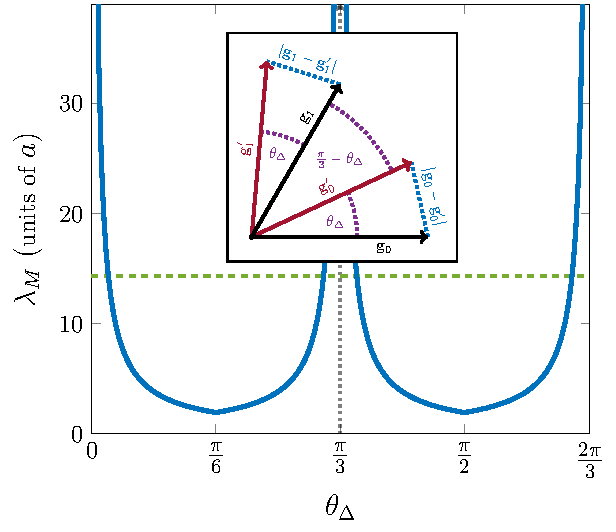
\includegraphics[width=0.55\textwidth]{ch5_kickit/fig6}
	\caption[Size of the resulting moir\'e super-structures as a function of the relative angle between the vortex and optical lattice.]{The dashed green line indicates the condensate radius. Inset: The different vectors in $\mathbf{k}$-space of the two lattices, with the optical lattice rotated by an angle $\theta_\Delta$. The $\mathbf{g}_{ll'} = |\mathbf{g}_l - \mathbf{g}_l'|$ vectors defining the dominant moir\'e wavelength are those for which the enclosed angle is smallest. }
	\label{fig:moire_lambda_1}
\end{figure}

    The appearance of the moir\'e vector in $\mathbf{k}$-space can be confirmed from the numerical simulations by looking at the compressible kinetic energy spectra which is given in Fig.~\ref{fig:dtheta_kspec}. Apart from the dominant peaks corresponding to the underlying triangular geometry of the Abrikosov lattice, which are independent of $\theta_\Delta$ (straight lines in Fig.~\ref{fig:dtheta_kspec}), a number of additional peaks appear. Their position is a function of the misalignment angle and the lowest wave-number that appears increases its value with increasing $\theta_\Delta$. This is consistent with the moir\'e model and the appearance of density structures of differing size. Furthermore, a symmetric repeat of this structure about the $\theta_\Delta=\pi/6$ point is also visible, which corresponds to the $\pi/3 - \theta_\Delta$ lattice vector component. The minimum wavelength observed agrees with the theoretically determined minimum value of $\lambda_M\approx 1.93\,a$ and all other values over the range of observed angles. Note that for the higher harmonics at larger wave-numbers similar behaviour exists and is also covered by the moir\'e model.

    To better observe the wavenumbers in the spectra, one can remove the background lattice spectrum. Corresponding to the system shown in Fig.~\ref{fig:dtheta_kspec_backg} this is given in Fig~\ref{fig:dtheta_kspec_backg}, with the peaks at $t=0$ removed. In this instance, lower interference patterns are more easily visualised, with a slight enhancement of higher orders. We can also observe the appearance of secondary interference patterns across low to high wavenumbers, though visibility quickly diminishes approaching higher wavenumbers. It should be noted that given sufficient time the higher order wave-numbers can influence the density dynamics, but the system remains dominated by the lowest wave-number. Due to coupling between adjacent modes in the system, all interference patterns become hard to discern after some time. As the condensate system is finite-sized a refocussing of the interference structures will eventually take place. However, the time-scales necessary to examine this were not investigated.

    %It is expected (but not investigated) that in the long time limit the interference patterns will eventually refocus and reappear. While the newly generated moir\'e interference patterns can also in turn create additional interferences with the background lattices, I will choose to ignore this effect for the reasons mentioned above regarding higher order wavenumbers.

	\begin{figure}
        \centering
		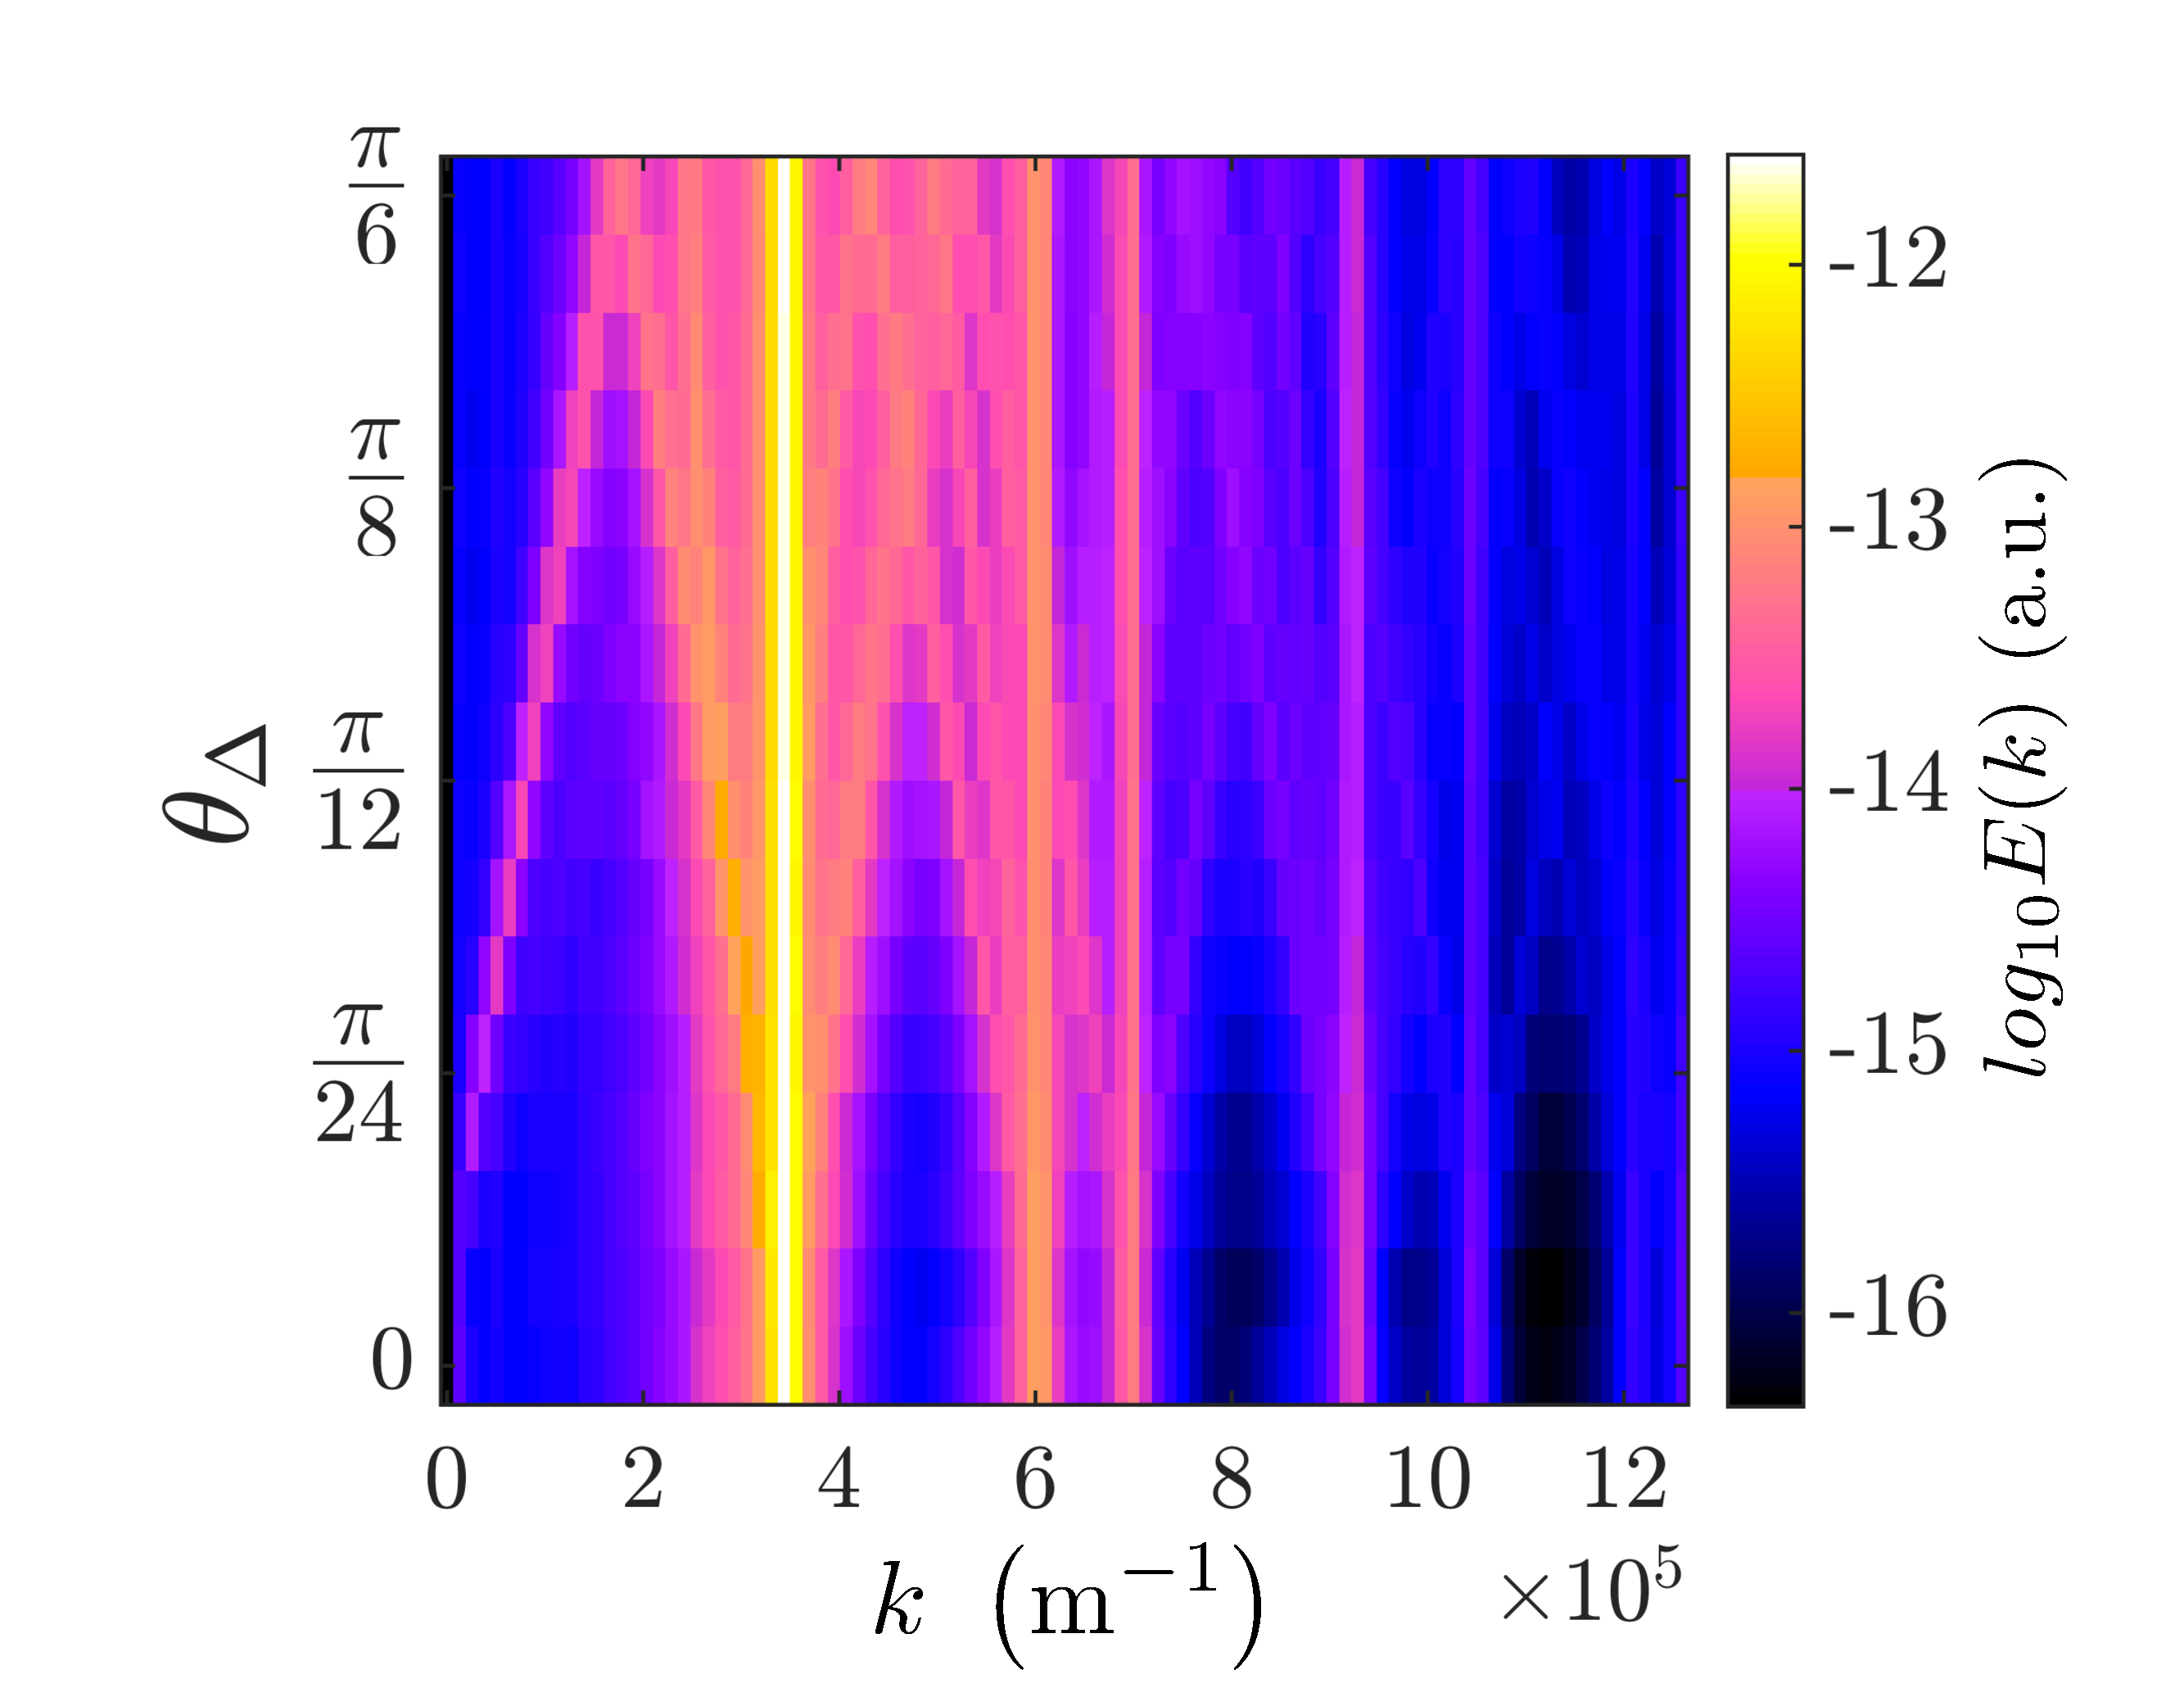
\includegraphics[width=0.65\textwidth]{ch5_kickit/fig7}
		\caption[Compressible kinetic energy spectrum as a function of $\theta_\Delta$.]{Compressible kinetic energy spectrum as a function of $\theta_\Delta$. All values are time-averaged over an interval $t=0$ s to $t=1$ s. The moir\'e peak corresponding to the lowest wave-number can be seen shifting to larger values for increasing angles and similar behavior is visible for the higher order components.}
		\label{fig:dtheta_kspec}
	\end{figure}
    \begin{figure}
        \centering
        \includegraphics[width=0.65\textwidth]{ch5_kickit/theta_sweep_diff}
        \caption[Compressible kinetic energy spectrum with the background structure removed.]{Compressible kinetic energy spectrum with the structures stemming from the static background removed. The effect of the moir\'e interference pattern for lower and higher modes is more clearly visible compared to Fig. \ref{fig:dtheta_kspec}.}
        \label{fig:dtheta_kspec_backg}
    \end{figure}

    In the following we will briefly discuss what happens for stronger kicking, or when the two lattices are non-commensurate. In the above the strength of the kicking pulse was chosen such that its perturbation only leads to a phase imprinting \cite{Vtx:Dobrek_pra_1999,BEC:Denschlag_science_2000}, with minimal change to the initial density. If one increases the kicking intensity the situation becomes quite different and one can see from Fig.~\ref{fig:kickp20k}$(a)$ that higher order wave-numbers become more strongly excited. This, in turn, leads to modulations of the condensate density at shorter wavelength and an example is shown in Figs.~\ref{fig:kickp20k}$(b)$-$(e)$, with the numerically calculated averaged spectra given in Fig.~\ref{fig:kick_compare_spec}. However, as for fully realistic experimental situations it is necessary to consider the heating of the condensate once the kicking becomes stronger, we restrict this investigation to low intensity pulses.

\begin{figure}
    \centering
	\includegraphics[width=0.75\textwidth]{ch5_kickit/fig8_2}
	\caption[Higher order modes induced by stronger kicking.]{(a) For a kicking strength of $V_0 = 5.4\times10^{-2}\mu$ for a non-rotating condensate higher order modes become non-negligible contributors to the compressible kinetic energy spectrum. This leads to the appearance of higher-order peaks which are visible in the condensate density. Close-ups of the density structures are shown for (b) 24 ms, (c) 36 ms, (d) 56 ms, and (e) 88 ms. Note that the larger structures in these plots are given by the optical lattice constant, $a_o$, which is set to the mean inter-vortex distance for the rapidly rotating condensate. In the presence of vortices this is anticipated to create many additional interferences.}
	\label{fig:kickp20k}
\end{figure}
\begin{figure}
    \centering
    \includegraphics[width=0.49\textwidth,page=1]{ch5_kickit/EKCEKI_novtx_power}
    \includegraphics[width=0.49\textwidth,page=2]{ch5_kickit/EKCEKI_novtx_power}
	\caption[Comparison of kinetic energy spectra for increased kicking strengths.]{For kicking pulses of $V_0 = (1.35,2.7,5.4)\times 10^{-2} \mu$ the kinetic energy spectra show a clear increase in higher order modes being excited for both compressible ($E_c$) and incompressible ($E_i$) cases with increased kicking strength.}\label{fig:kick_compare_spec}
\end{figure}

    A situation where the optical and the vortex lattice have different lattice constants can be imagined to appear naturally due to experimental uncertainties. Defining $a_o = a_v(1+\epsilon)$ the expression in Eq.~\eqref{eq:InterferenceVectors} can be calculated to be
    \begin{equation}
    	\lambda_M = \frac{a_v(1+\epsilon)}{\sqrt{2(1+\epsilon)(1-\cos\theta) + \epsilon^2}}
    	\label{eqn:moire_size_eps}
    \end{equation}
    which reduces to Eq.~\eqref{eqn:moire_size} for $\epsilon=0$. Evaluating this expression for $\epsilon = (-0.1,0,0.1)$ shows that the largest moir\'e wavelength changes slightly for small values of $\epsilon$, but it remains distinct enough from the higher order wavelengths to stay visible in the evolution (see Fig.~\ref{fig:epsilon}). This ensures that the system examined here is experimentally realistic. For large deviations of the lattice constant, the assumption of the largest moir\'e wavevector playing the dominant role is no longer valid, as many wavevectors approach comparable scales.

    \begin{figure}
        \centering
        \includegraphics[width=0.5\textwidth]{ch5_kickit/Moire_higherk_epsrange}
    	\caption[Moir\'e wavelengths for imperfect lattice alignment.]{Small deviations for $\epsilon$ gives minor changes to the induced moir\'e wavelength.}\label{fig:epsilon}
    \end{figure}


\section{Vortex dynamics following a kick}
While we have concentrated mostly on the phonon modes of the condensate density it is necessary to also examine the result of kicking on the vortex lattice. Fig.~\ref{fig:kickit_traj} shows the densities and trajectories in the co-rotating frame for a kick of $\theta_{\Delta}=\pi (1/60, 1/10)$. Some deviation from solid-body rotation is observed at the edge of the examined vortex region, but the central vortex regions show almost no variation from their ideal lattice positions.
\begin{figure}
    \centering
    \includegraphics[width=0.9\textwidth]{ch5_kickit/Trajectory_after_kick_theta0_15_3offset}
	\caption[Vortex densities and trajectories following a kick.]{The condensate densities are shown for times $t=(20,200)$ ms, and for $\theta_\Delta = ( 3^{\textrm{o}},18^{\textrm{o}})$ (top and bottom). The resulting trajectories of the vortices show minimal deviation from their initial lattice positions over 2 seconds of time evolution.}\label{fig:kickit_traj}
\end{figure}

Both cases demonstrate the same overall dynamics, with the vortex lattice showing extreme robustness against the phononic perturbances that build following a kick. The moir\'e superlattice forms on top of the existing condensate density.

\section{Conclusions and outlook}\label{sec:ch5_conc}
The purpose of the previous work was to investigate the effect of a kicked optical lattice potential with a well defined periodicity on a vortex lattice having its own periodic structure. As observed in the incompressible spectrum, kicking gave negligible effect to the vortex positions, with the lattice remaining well defined with near constant spacings, even in the long time limit. The optical lattice kicks solely modified the background density around the vortex cores. One could observe that the vortex lattice remains incredibly stable and strongly resilient to perturbations and modulations in density. Given the stability of the lattice, it can be expected that even for a finite number of kicks, the lattice will remain mostly unbroken. It can also be expected that heating effects would play a role in destabilising the condensate, and to determine any long-term realistic behavior from this system, including the treatment of a non-negligible thermal cloud contribution would be necessary.

The kinetic energy spectra provided a useful tool to investigate the order of the imparted wavenumbers following a kick, and were very closely matched with the results from moir\'e interference theory. The existence of this moir\'e interference effect has some nice consequences. It can, for example, be thought of as a tool to test the periodicity of a structure that is too small to resolve without time of flight. In general, this technique may be used on other types of periodic structures, for example crossed solitons in 2D condensates \cite{BEC:Morgan_soliton_2013}. As optical lattices can offer a large number of free parameters (lattice constant, amplitude, misalignment, geometry, \ldots), a full toolbox can be developed from this technique. This could potentially be used for probing condensate systems, applying well-defined structures onto stationary condensates, and for generating the aforementioned interferences in the presence of an underlying periodicity.

%As an extension of work on large Abrikosov lattices, some preliminary work in zig-zag and linear vortex crystals, in conjunction with A.~Barahmi and Th.~Busch, showed that without well defined periodic behaviour there is negligible observation of any peaks in the compressible energy spectrum. As such, there were no discernible moir\'e patterns in the density. It is expected that for such an effect to be useful highly periodic systems are required, with well defined wave-vectors. It remains an open question as to whether this can be used in a realistic experimental setting for such a purpose.

While in my thesis proposal the system discussed in this chapter was suggested to investigate delta-kicked chaotic dynamics, it became clear very quickly that the robustness of the vortex lattice with respect to realistic kicking strengths did not allow for significant vortex dynamics. Nevertheless, an investigation into periodic kicking is still an interesting (and numerically even more challenging) endeavor. As vortex lattices feature a well-defined rotation rate and 6-fold symmetry, the system rotates to a symmetric position every $\pi/3$. Providing a periodic kick at this rate, would therefore allow the lattice to always have the same alignment angle, at least for a number of kick repetitions.

\fi
%%%%%%%%%%%%%%%%%%%%%%%%%%%%%%%%%%%%%%
\newif\ifdefect
\defecttrue
\ifdefect
    \chapter{Defect engineering}
        %%%%%%%%%%%%%%%%%%%%PAPER
%%%%%%%%%%%%%%%%%%%%%%%%%%%%%%%%%%%%%%%%%%%%%%%%%%%%%%%%%%%%%%%%%%%%%%%%%%%%%%%%%%%%%%%%%%%%%%%%%%%%%%%%%%%%%%%%%%%%%%%%%%%%%%%%%%%%%%%%%%%%%
\subsection{Rapidly rotating BEC}
%%%%%%%%%%%%%%%%%%%%%%%%%%%%%%%%%%%%%%%%%%%%%%%%%%%%%%%%%%%%%%%%%%%%%%%%%%%%%%%%%%%%%%%%%%%%%%%%%%%%%%%%%%%%%%%%%%%%%%%%%%%%%%%%%%%%%%%%%%%%%
For this work, we numerically solve the Gross-Pitaevskii equation in two dimensions, assuming a strong confinement along the third axis.
This allows all dynamics to be restricted to the $xy$ plane, with vortices behaving as charged particles in a neutral background. In the
frame corotating with the condensate, this can be modeled as
\begin{equation}
	 i\hbar\partial_t \Psi\left(\mathbf{x},t\right) = \left[ -\frac{\hbar^2}{2m}\nabla^2 + V\left(\mathbf{x}\right) + g\vert \Psi\left(\mathbf{x},t\right) \vert^2 - \Omega L_z \right]\Psi\left(\mathbf{x},t\right)
\end{equation}
where $V\left(\mathbf{x}\right)$ is the trapping geometry, $\Omega$ is the trap rotation frequency, and $L_z$ is the angular momentum
operator along the $z$-direction. For the rapidly rotating case, the vortices form an ordered triangular lattice, that rotates equivalently
to a solid-body in the large number limit. Deviations from the solid-body rotation can be seen for trajectories in the limit of long times
(~10 s). This is very likely due to long-wavelength Tkachenko modes in the condensate, and following the analysis of [Baym, Tk modes of vtx latt in rr BEC]
has a frequency much longer than the lifetime of the system for our given rotation rate.
%However, due to the density inhomogeneities of a harmonically trapped condensate, and the likelihood of shearing this is (I think) expected.
The lattice is well ordered and behaved at timescales on the order of upto few seconds, as well as away from the condensate edges, and so we
will restrict our analysis therein.

As condensates are highly controllable in the lab (cite many papers), we consider the use of many common experimental techniques to engineer
specific states otherwise difficult in solid-state materials. One such set of systems are those of crystals with controllable defects, which
although (relatively) easily created classically (cite bead packing, etc), are difficult experimentally in quantum systems due to the sizes
of interatomic spacings. Here we propose the use of phase-imprinting (cite) as a means of achieving such defects in a Bose-Einstein
condensate. Through direct manipulation of the condensate phase, vortices may be added or removed from specific locations in the system.

%%%%%%%%%%%%%%%%%%%%%%%%%%%%%%%%%%%%%%%%%%%%%%%%%%%%%%%%%%%%%%%%%%%%%%%%%%%%%%%%%%%%%%%%%%%%%%%%%%%%%%%%%%%%%%%%%%%%%%%%%%%%%%%%%%%%%%%%%%%%%
\subsection{Order/disorder}
%%%%%%%%%%%%%%%%%%%%%%%%%%%%%%%%%%%%%%%%%%%%%%%%%%%%%%%%%%%%%%%%%%%%%%%%%%%%%%%%%%%%%%%%%%%%%%%%%%%%%%%%%%%%%%%%%%%%%%%%%%%%%%%%%%%%%%%%%%%%%
Given the localised defect disturbs the lattice after sufficiently long times, we can examine if the lattice moves from global ordered to
disordered following the addition or removal of another site over the course of time. For a two-dimensional material, KTHNY theory describes
the transitions from a solid crystalline to amorphous fluid phase, via an intermediate hexatic phase. This state is generally characterised
by the translational and orientational correlation functions long-ranged behaviour. As we have an inhomogeneous density profile, and thus
lattice outside a given radius, the use of translational correlations does not make much sense. Orientational correlations however, which
measure how the lattice aligns to a particular angle, should suffice when combined with the density structure factor,
$S = \int d\mathbf{r}e^{i\mathbf{k}\cdot\mathbf{r}}|\Psi|^2$. True crystalline behaviour is given by orientational constant values, with
power-law decay is expected for a hexatic phase, and exponential decay for an amorphous fluid (neglecting translational correlations).

%%%%%%%%%%%%%%%%%%%%%%%%%%%%%%%%%%%%%%%%%%%%%%%%%%%%%%%%%%%%%%%%%%%%%%%%%%%%%%%%%%%%%%%%%%%%%%%%%%%%%%%%%%%%%%%%%%%%%%%%%%%%%%%%%%%%%%%%%%%%%
\subsection{Phase imprinting defects}
%%%%%%%%%%%%%%%%%%%%%%%%%%%%%%%%%%%%%%%%%%%%%%%%%%%%%%%%%%%%%%%%%%%%%%%%%%%%%%%%%%%%%%%%%%%%%%%%%%%%%%%%%%%%%%%%%%%%%%%%%%%%%%%%%%%%%%%%%%%%%
Phase imprinting has been shown as an effective tool for the creation of vortices within a Bose-Einstein condensate (cite). The signature of
a quantum vortex is given by a phase singularity, around which the phase winds through $\pm 2\pi$, depending upon the direct of rotation.
Through the use of the phase imprinting method, we can eliminate a vortex from the lattice by applying the correct phase profile. To
eliminate a vortex from the lattice we need only to apply the opposite phase winding to that of the vortex to be eliminated. The
instantaneous application of a phase singularity to the condensate will create phonon modes in the density, as will the annihilation event.
Since the induced phonons have been shown to yield minimal impact on the vortex lattice structure <ref my paper>, we can safely
ignore their contribution. The removal of a vortex from the lattice introduces a vacancy to the system.


We model the vortex lattice as a graph, where each vortex represents a node, and edges are given by nearest neighbours at most separated by
a distance $a_v$, for a triangular lattice configuration, or $\sqrt{2}a_v$ for a square lattice (see Fig. \ref{fig:vtxdist}). The inclusion
of the square lattice distance is chosen so that upon removal, the vortices can reconfigure their arrangement locally, and may move from
triangular to square geometries. As they behave like Coulombic particles with a profile that falls off as $r^{-1}$ we can consider that any
interactions outside these distances to be negligible.

\subsubsection{Lattice vacancy}
%%%%%%%%%%%%%%%%%%%%%%%%%%%%%%%%%%%%%%%%%%%%%%%%%%%%%%%%%%%%%%%%%%%%%%%%%%%%%%%%%%%%%%%%%%%%%%%%%%%%%%%%%%%%%%%%%%%%%%%%%%%%%%%%%%%%%%%%%%%%%
The removal of a vortex from the vortex is thus expected to affect only the nearest neighbours by altering their velocity well, with the
overall angular momentum of the condensate decremented by a single quantum. The resulting vacancy, following a vortex removal, remains
localised to its respective position within the lattice for long times, regardless of initial placement (assuming not at edge)
(see Fig. \ref{fig:trajectory}). The
resulting stability of the nearest neighbours follows a decay of the honeycomb-like structure akin to that described by [statistical
topology of perturbed two-dimensional lattices]. Given enough time, this structure decays via one of the three possible means, creating a
locally disordered region with a grain boundary/disclination/dislocation? evident of the lattice change. However, even for long times, the
overall vortex lattice remains well structured, as evidenced by examining correlation functions of the vortex positions for both two-body,
and orientational correlations.

After the vortex removal, the system remains in a stable configuration, for a period on the order of 100+ ms (see Fig. \ref{fig:voronoi_area},
\ref{fig:voronoi_100ms}), after which the vortices begin to deviate from their lattice positions and attempt to fill the vacancy and balance
the inter-vortex forces. Removing vortices at different positions in the lattice shows similar behaviour, with the effect on the velocity profile and trajectories of other vortices being mostly localised around the removal site. Tracking the vortex distances traveled for different removal locations, and for a different number of removed vortices shows how much we disturb the underlying lattice (see \ref{fig:vtxdist}).

\subsubsection{Lattice overpopulation}
%%%%%%%%%%%%%%%%%%%%%%%%%%%%%%%%%%%%%%%%%%%%%%%%%%%%%%%%%%%%%%%%%%%%%%%%%%%%%%%%%%%%%%%%%%%%%%%%%%%%%%%%%%%%%%%%%%%%%%%%%%%%%%%%%%%%%%%%%%%%%
Similarly to removing a vortex from the lattice, we can also add one. By choosing a pre-existing vortex and adding a like-signed phase
winding, we can create multiply charged vortices in the condensate, where the vortex has a winding of $2\pi l$, with $l$ as the vortex
charge. Multiply charged vortices are usually unstable in condensates, as it is more energetically favourable to have two singly charged
vortices, than a single doubly charged vortex, as the energy increases with $l^2$. Thus, an $l$-charged vortex is expected to instead decay
into $l$ singly-charged vortices due to the presence of complex eigenmodes in the Bogoliubov spectrum \cite{VTX:Kawaguchi_pra_2004}.

Here we have taken our lattice of $l=1$ vortices, and given an additional charge to a single vortex to examine the decay process. However,
the presence of the lattice suppresses the decay process for long times (order of seconds) compared to that of in a condensate without vortex
lattice. The doubly charged vortex remains stable on the order of seconds even away from the lattice centre (though does decay eventually).
The additional velocity profile locally causes the nearest neighbouring vortices to rotate faster than the solid-body rotation rate of the
whole lattice, causing a local shearing of the lattice structure. As with the vacancies, the use of correlation functions allowed us to
examine the short and long-range order of the lattice.

Voronoi diagrams of the resulting lattice show a stable doubly charged vortex position, with show twisting of the lattice about this central
point.

\begin{figure}[tb]
	\includegraphics[width=0.49\textwidth]{imgs/DoubleCharge/add161/voronoi}
	\includegraphics[width=0.49\textwidth]{imgs/DoubleCharge/add161remove207/voronoi}
	\caption{(top) Doubly charged central vortex. Doubly charged vortex remains stable, and retains 6-fold
	symmetry of vortex lattice. (bottom) Doubly charged central vortex, and removal of nearby vortex. Doubly charged vortex remains stable, and forms 8-fold
	symmetry of vortex neighbours.}
	\label{fig:voronoi_double}
\end{figure}



%%%%%%%%%%%%%%%%%%%%%%%%%%%%%%%%%%%%%%%%%%%%%%%%%%%%%%%%%%%%%%%%%%%%%%%%%%%%%%%%%%%%%%%%%%%%%%%%%%%%%%%%%%%%%%%%%%%%%%%%%%%%%%%%%%%%%%%%%%%%%
\subsection{Things to note}
%%%%%%%%%%%%%%%%%%%%%%%%%%%%%%%%%%%%%%%%%%%%%%%%%%%%%%%%%%%%%%%%%%%%%%%%%%%%%%%%%%%%%%%%%%%%%%%%%%%%%%%%%%%%%%%%%%%%%%%%%%%%%%%%%%%%%%%%%%%%%

\begin{itemize}
\item Localised disturbances: introducing vacancy to lattice causes it to travel with lattice. Change in velocity profile only affects 6
nearest neighbours on moderate timescales.
\item Long range hexatic phase has short range translational order (exp drop off), but constant orientational order -> is this such a phase?
\end{itemize}

%%%%%%%%%%%%%%%%%%%%%%%%%%%%%%%%%%%%%%%%%%%%%%%%%%%%%%%%%%%%%%%%%%%%%%%%%%%%%%%%%%%%%%%%%%%%%%%%%%%%%%%%%%%%%%%%%%%%%%%%%%%%%%%%%%%%%%%%%%%%%
\subsection{Correlations}
%%%%%%%%%%%%%%%%%%%%%%%%%%%%%%%%%%%%%%%%%%%%%%%%%%%%%%%%%%%%%%%%%%%%%%%%%%%%%%%%%%%%%%%%%%%%%%%%%%%%%%%%%%%%%%%%%%%%%%%%%%%%%%%%%%%%%%%%%%%%%
According to KTHNY theory for a 2D material the transition from a solid crystal to liquid phase is mediated through an intermediary hexatic
phase. This phase is usually characterised by the translational and orientational correlation functions. Given the lack of translation order
in a harmonically trapped condensate, we restrict our analysis to the orientational correlation function, $g_6$ given by
\iffalse
\begin{equation}
	\begin{aligned}
		g_6(|\mathbf{r}_i - \mathbf{r}_j|) &= \\ \frac{1}{N(r)}\displaystyle\sum_{i}^{N(r)}\displaystyle\sum_{j}^{N(r)} & \left(\frac{1}{n_j}\displaystyle\sum_{k}^{n_j}\exp(6\mathrm{i}\theta_{jk}) \right)\left(\frac{1}{n_i}\displaystyle\sum_{l}^{n_i}\exp(6\mathrm{i}\theta_{il}) \right)^{*}
	\end{aligned}
\end{equation}
\fi
\begin{equation}
	g_6(r) = \frac{1}{N(r)}\displaystyle\sum\limits_{i,j}^{N(r)}\psi_6(\mathbf{r}_i)\psi_6^{*}(\mathbf{r}_j),
\end{equation}
with
\begin{equation}
	\psi_6(|\mathbf{r}_{i} - \mathbf{r}_{j}|) = \frac{1}{n_i}\displaystyle\sum\limits_j^{n_i}\exp(6\mathrm{i}(\theta_i - \theta_j)),
\end{equation}
where $\psi_6$ is the orientational order parameter, and $j$ is over the nearest neighbouring vortices.

According to [] the decay in correlations for both translational and orientational order give indication to the material phase. In a
two-dimensional material the positional order is expected to decay algebraically as a function of radius, differing from that of a
three-dimensional material, which tends to a constant value. Here we examine the orientational correlation function as a measure of the
order of a "vortex unit cell", consisting of the angle made by nearest neighbours to an individual vortex. For a perfectly ordered
triangular lattice this value will tend to 1. To maintain constant vortex areal density, we choose vortices defined at a radius of
$r=2\times 10^4$ m from the centre, which give an almost uniform lattice constant for our system parameters.

\begin{itemize}
\item Crystalline: $\lim\limits_{r\rightarrow \infty}\hat{g}_T(r) \neq 0$, $\lim\limits_{r\rightarrow \infty}\hat{g}_6(r) \neq 0$
\item Long-range hexatic: $\hat{g}_T(r) \approx _{r\rightarrow \infty} \exp(-r/\xi_T) $, $\lim\limits_{r\rightarrow \infty}\hat{g}_6(r) \neq 0$
\item Power-law hexatic: $\hat{g}_T(r) \approx _{r\rightarrow \infty} \exp(-r/\xi_T) $, $\hat{g}_6(r) \approx _{r\rightarrow \infty} 1/r^{\eta_6}$
\item Amorphous: $\hat{g}_T(r) \approx _{r\rightarrow \infty} \exp(-r/\xi_T) $, $\hat{g}_6(r) \approx _{r\rightarrow \infty} \exp(-r/\xi_6) $
\end{itemize}
Hat means normalised (see page 119 of order in two dim binary random arrays, Nelson et al.)


%%%%%%%%%%%%%%%%%%%%%%%%%%%%%%%%%%%%%%%%%%%%%%%%%%%%%%%%%%%%%%%%%%%%%%%%%%%%%%%%%%%%%%%%%%%%%%%%%%%%%%%%%%%%%%%%%%%%%%%%%%%%%%%%%%%%%%%%%%%%%
\subsection{Numerics and results}\label{sec:numerics}
%%%%%%%%%%%%%%%%%%%%%%%%%%%%%%%%%%%%%%%%%%%%%%%%%%%%%%%%%%%%%%%%%%%%%%%%%%%%%%%%%%%%%%%%%%%%%%%%%%%%%%%%%%%%%%%%%%%%%%%%%%%%%%%%%%%%%%%%%%%%%

Each vortex position was found by summing over adjacent grid sites, and looking for a $2\pi$ phase winding. This gave a vortex position
estimated to the numerical grid. A least-squares fit was performed to more accurately determine the vortex core. Vortices closest the centre
of the condensate were considered to ensure an almost uniform inter-vortex spacing, giving minimal deviation in lattice constant, $a_v$. Each
vortex was assigned a unique identifier (UID) to allow for it to be tracked individually over the course of the simulations, with the initial
configuration presented in the graph [ref graph]. By noting these UIDs, vortices can be individually selected for removal by applying the
global $2\pi$ phase winding in the opposing direction, centered on the core.

The trajectory plots show very small global effect on the core positions, with a disturbance localised in a region centered on the removed
core. By removing vortices in different locations on the condensate we see similar behaviour, with the trajectories modified in a region
around the removed vortex. The removal of two vortex adjacent cores can be seen to crate a greater disturbance, as expected, with the
trajectories of the surrounding vortices no longer following an almost circular path (more like hexagonal), but taking on other geometric
path shapes. For two nn vortices the path becomes an almost rhombic shape, with nnn forming an elongated hexagon (as to be expected). For 3
nn, the resulting trajectories follow a triangular pattern of the same orientation as the removed vortices. For the removal of an entire 7
vortex cell, the formed pattern is star shaped.

TODO:
Calculate incompressible kinetic energy spectrum for each case, and see if useful. RESULT: It wasn't.
Calculate $S(k) = |\Psi(k)|^2$ for condensate densities, not just vortex positions, for comparison. RESULT: looks strange, even in untouched
case. Arcs exist in all cases, but with interference lines.

The impact on the overall distances traveled by each vortex as a result of the dislocations is given in figure [some fig].

%\iffalse
\begin{figure}[tb]
	\includegraphics[width=0.48\textwidth]{imgs/mono}
	\caption{The oscillation of the mean-radius of the condensate after the addition of vortices (positive) or antivortices (negative) with
	different imprinted windings. The oscillation mode shows an exact match for a 2D non-rotating condensate of $2\omega_{\perp}$ for all cases.}
\end{figure}
%\fi

\begin{figure}[tb]
	\includegraphics[width=0.48\textwidth]{imgs/FFT_density_linear_cell}
	\caption{Density structure factor within 4*pi/(sqrt(3)*d0).}
\end{figure}

%\begin{figure}[h!]
%	\includegraphics[width=0.48\textwidth]{imgs/FFT_density}
%	\caption{Density structure factor.}
%\end{figure}

\begin{figure}[tb]
	\includegraphics[width=0.48\textwidth]{imgs/RDF_time_gp}
	\caption{Radial distribution function over time after removing vortex from lattice centre. }
\end{figure}


\begin{figure}[tb]
	\includegraphics[width=0.48\textwidth]{imgs/graph86}
	\caption{Condensates vortices treated as nodes in a graph. Edges are drawn between nearest neighbours.}
\end{figure}
%\fi
%%%%%%%%%%%%%%%%%%%%%%%%%%%%%%%%%%%%%%%%%%%%%%%%%%%%%%%%%%%%%%%%%%%%%%%%%%%%%%%%%%%%%%%%%%%%%%%%%%%%%%%%%%%%%%%%%%%%%%%%%%%%%%%%%%%%%%%%%%%%%
\section{Conclusions}\label{sec:conc}
%%%%%%%%%%%%%%%%%%%%%%%%%%%%%%%%%%%%%%%%%%%%%%%%%%%%%%%%%%%%%%%%%%%%%%%%%%%%%%%%%%%%%%%%%%%%%%%%%%%%%%%%%%%%%%%%%%%%%%%%%%%%%%%%%%%%%%%%%%%%%

The removal of a vortex from the lattice creates a stable vacancy site, which in the corotating frame, travels with the lattice for some time
before decaying into paired 5 and 7 nearest neighbour disclinations. These disclination pairs can be viewed as as an edge dislocation in the
lattice. The resulting grain boundary breaks the 6-fold symmetry of the triangular lattice. The removal of the single vortex also removes the
velocity profile associated with the vortex at that location. The local velocity near the vacancy will be less than the solid-body behaviour
of the lattice. This causes the nearest neighbour vortices to rotate slower than the condensate, locally creating a strain/shear? on the
lattice. Local competition to fill the vacancy ensures its long-lived stability. The removal of the central vortex creates a local honeycomb
lattice structure, which according to [stat top of 2d lattice] will decay (following perturbation) via three possible processes.

Increasing the charge of a vortex by applying the same signed phase winding to a vortex core creates a stable doubly charged vortex for long
times (seconds). This, like the stable vacancy, seems to be stable at any range of positions (but decays faster at outskirts). The additional
velocity field shears the lattice, with the resulting correlations showing long-range power-law behaviour. This is usually indicative of a
power-law hexatic phase. Given the lack of true translational order in a harmonically trapped vortex lattice, it remains more instructive to
investigate the static structure factor of the system. The hexatic phase is expected to show spreading of the Fourier peaks into arcs. Here,
though we see such spreading, it is not entirely arc-like, and does not match entirely with the expectations of a hexatic phase.



%%%%%%%%%%%%%%%%%%%%%%%%%%%%%%%%%%%%%%%%%%%%%%%%%%%%%%%%%%%%%%%%%%%%%%%%%%%%%%%%%%

        %%%%%%%%%%%%%%%%%%%%%%%%%%%%%%%%%%%%%%%%%%%%%%%%%%%%%%%%%%%%%%%%%%%%%%%%%%%%%%%%%%%%%%%%%%%%%%%%%%%%%%%%%%%%%%%%%%%%%%%%%%%%%%%%%%%%%%%%%%%%%
\section{Phase imprinting defects}\label{sec:phase}
%%%%%%%%%%%%%%%%%%%%%%%%%%%%%%%%%%%%%%%%%%%%%%%%%%%%%%%%%%%%%%%%%%%%%%%%%%%%%%%%%%%%%%%%%%%%%%%%%%%%%%%%%%%%%%%%%%%%%%%%%%%%%%%%%%%%%%%%%%%%%

Where previously I added an optical potential to the Hamiltonian for a short time during the evolution, here I directly engineer the wavefunction phase. For the previously chosen kicking strengths and timestep, the limiting values of the phase change are $\approx 0.2 < \phi < \approx 0.94$. This is determined by writing the phase as
\begin{equation}
    e^{i\phi} \mapsto \exp\left(-i\frac{V_{\textrm{opt}}dt}{\hbar}\right),
\end{equation}
and filling in for the defined simulation values. Thus, for a much stronger phase change a longer lasting pulse, or a greater amplitude are two possible contenders. However, as discussed previously, neither are suitable candidates in this system, given the lattice rotation, as well as the excitation of higher-order wavenumbers. With the use of direct phase imprinting we can realise arbitrary phase patterns on the condensate. Previously the vortex lattice was unaffected by the imprint; here I attempt to destroy the vortex lattice by directly engineering the opposite phase winding profile atop a lattice vortex. This has the distinct advantage of locally erasing a vortex and disordering the lattice. I will now discuss this method.

Phase imprinting is a technique that applies a spatially inhomogeneous optical potential across a condensate in such a way that the phase is modified to a desired form. As a consequence the density distribution will adjust itself and in ground state condensates dark solitons \cite{BEC:Denschlag_science_2000}, as well as vortices \cite{Vtx:Dobrek_pra_1999} have been created this way. For the latter the signature is given by a phase singularity, around which the phase winds through $\pm 2\pi$, depending upon the direction of rotation.

The phase imprinting method can also be used to annihilate a vortex from the lattice by applying a phase profile of opposite winding, removing the phase singularity.  This will leave the condensate with a density depletion at the prior location of the phase singularity. Without the singularity this depletion will fill in and excite phonon modes in the condensate during time evolution. This method will form the basis for which the further discussions and analysis are performed on the vortex carrying condensate.


%%%%%%%%%%%%%%%%%%%%%%%%%%%%%%%%%%%%%%%%%%%%%%%%%%%%%%%%%%%%%%%%%%%%%%%%%%%%%%%%%%%%%%%%%%%%%%%%%%%%%%%%%%%%%%%%%%%%%%%%%%%%%%%%%%%%%%%%%%%%%
\section{Model}\label{sec:model}
%%%%%%%%%%%%%%%%%%%%%%%%%%%%%%%%%%%%%%%%%%%%%%%%%%%%%%%%%%%%%%%%%%%%%%%%%%%%%%%%%%%%%%%%%%%%%%%%%%%%%%%%%%%%%%%%%%%%%%%%%%%%%%%%%%%%%%%%%%%%%

To investigate the evolution of a perturbed vortex lattice we numerically solve the Gross--Pitaevskii equation in two dimensions, assuming a strong confinement along the third axis. This allows to restrict the dynamics to the $x$--$y$ plane and focus fully on the Abrikosov lattice geometry. Experimental setups in lower dimensions are currently available \cite{BEC:Stock_lpl_2004,BEC:Seo_jkps_2014,BEC:Chomaz_natcom_2015} and in the frame co-rotating with the condensate, the non-linear mean field equation governing the BEC wave-function is given by
\begin{align}
i\hbar\partial_t \Psi(\mathbf{r},t) = \Big[&-\frac{\hbar^2}{2m}\nabla^2 + V\left(\mathbf{x}\right) \nonumber\\
&+ g\vert \Psi(\mathbf{r},t) \vert^2- \Omega L_z \Big]\Psi(\mathbf{r},t)
\end{align}
Here $V\left(\mathbf{x}\right)$ is the trapping geometry, $\Omega$ is the trap rotation frequency, and $L_z$ is the angular momentum operator along the $z$-direction. For the rapidly rotating case, the vortices form an ordered triangular lattice, that rotates equivalently to a solid-body in the large number limit. Simulating a large vortex lattice is a difficult numerical problem, due to the required grid size to resolve all aspects of the system both in position and momentum space. Thus, an advanced numerical technique is required to obtain solutions in a reasonable timescale. We have developed and made use of ``GPUE'' \cite{GPUEDOI}, an open-sourced, graphics processing unit (GPU) enabled Gross--Pitaevskii equation solver. This software allows for the solution of dynamical behaviours of linear and non-linear Schr\"odinger systems in significantly shorter times than alternative implementations \cite{AO:Morgan_pra_2013,Wittekblog_2016}.

%\subsection{Lattice order}

From the vortex lattice groundstate wavefunction we consider each individual vortex as an effective particle. As the unperturbed lattice is well ordered near the condensate center at timescales of up to several seconds we restrict our analysis therein. Given the coordinate locations for each individual vortex it is possible to calculate statistical quantities on the quality of the resulting lattice. Each vortex position was found by summing over adjacent grid sites, and looking for a $2\pi$ phase winding. This gave a vortex position estimated to the numerical grid. A least-squares fit was then performed to more accurately determine the vortex core to sub-grid resolution.

As we have an inhomogeneous density profile due to the harmonic confinement, and a system with a finite size, the use of translational correlations does not make much sense. Orientational correlations however, which measure how the lattice aligns along a particular angle may be useful. We calculate the orientational correlation function as
\begin{equation}
	g_6(r) = \frac{1}{N(r)}\displaystyle\sum\limits_{i,j}^{N(r)}\psi_6(\mathbf{r}_i)\psi_6^{*}(\mathbf{r}_j),
\end{equation}
with
\begin{equation}
	\psi_6(|\mathbf{r}_{i} - \mathbf{r}_{j}|) = \frac{1}{n_i}\displaystyle\sum\limits_j^{n_i}\exp(6\mathrm{i}(\theta_i - \theta_j)),
\end{equation}
where $\psi_6$ is the orientational order parameter, and $j$ is over the nearest neighbouring vortices.

We examine the orientational correlation function as a measure of the order of a ``vortex unit cell'', consisting of the angle made by nearest neighbours to an individual vortex. For a perfectly ordered triangular lattice this value will tend to 1. To maintain constant vortex areal density, we choose vortices defined at a radius of up to $r=2\times 10^{-4}$ m from the centre, which give an almost uniform lattice constant for our system parameters.

Additionally, we make use of the Delaunay triangulation of the vortex lattice to determine the occurrence of topological defects within the lattice. Delaunay triangulation generates a mesh from the vortex positions, wherein we examine the resulting triangulation for the appearance of non 6-fold connected vortices. When combined with other defects, such as a paired 5 and 7-fold connected vortex, these form dislocations in the crystal structure. These structures are countable, allowing us to directly determine the effect a perturbation has on the lattice.

\subsection{Few vortex dynamics}

To fully understand the effect of removing a vortex from the lattice system, let us first investigate the effects from removing the vorticity from a single vortex carrying condensate. Since the presence of vorticity requires the presence of a phase singularity, vortices possess the characteristic density depletion in their centre, which becomes unstable once the angular momentum is removed. The results of such a process can be seen in Fig.~\ref{fig:annihilation_1vtx}, and, as expected, the depletion of the condensate density fills in after the vortex phase is removed. An examination of the squared-radial expectation value, $\langle r^2 \rangle$, where $r^2 = x^2 + y^2$, shows that removing the vortex from the condensate excites a breathing mode, at the expected frequency of $2\omega_\perp$ for a two-dimensional system. The change in energy of the condensate is shown via the ratio of compressible (phonon) and incompressible (vortex) kinetic energy spectra given by Fig.~\ref{fig:kinspec}. As the vortex is annihilated we see a drop in the ratio of energies to favor a lower incompressible-to-compressible values for higher wavenumbers, resulting from the creation of a sound wave.

\begin{figure} \centering
    \includegraphics[width=0.55\textwidth]{ch6_phasegineer/imgs/NEWPICS/1vtx_remove1_centred2}
    \caption{The evolution of the condensate density and phase is shown for the initial state, and after 10 ms of evolution. The application of the phase creates sound waves which expand radially from the point of application. The line-plot shows the squared-radial expectation value which indicates the excitation of a breathing mode at $\omega_B = 2\omega_\perp$.}\label{fig:annihilation_1vtx}
\end{figure}

\begin{figure} \centering
    \includegraphics[width=0.55\textwidth]{ch6_phasegineer/tikz/EKt}
    \caption{The ratio of incompressible to compressible energies at times $t=0$ (solid) and $t=\tau$ (dashed), where $\tau=10$ ms. Initially the incompressible energy is greater than the compressible due to the presence of a vortex giving values greater than unity for all $k$. After application of the phase profile, the vortex is annihilated, with the energy released as phonons, indicated by a decrease in incompressible energy for higher $k$ values.}\label{fig:kinspec}
\end{figure}

\begin{figure} \centering
    \includegraphics[width=0.55\textwidth]{ch6_phasegineer/imgs/1vtx_remove1_uncentred}
    \caption{The condensate evolution following an uncentered phase imprint. For an imprint that is of the order of the healing length from centre to centre, the annihilation occurs during the evolution (a,b). However, beyond this distance, we create an antivortex which travels with the pre-existing vortex and circulates the condensate (c,d,e).}\label{fig:annihilation_1vtx_uncentred}
\end{figure}

While the above suggest that erasing vortices is a straightforward and controllable process, this assumption needs to be checked for the situation where the imprinted phase and the exiting phase are not perfectly centered on each other.
%In addition to the ideal situation of perfect erasing of a centered vortex as discussed above, an additional situation is of interest: what happens when the erasing phase is not centred on the phase singularity (see Fig.~\ref{fig:annihilation_1vtx_uncentred}).
%As one can see
This situation is shown in Fig.~\ref{fig:annihilation_1vtx_uncentred} and one finds that cases where the imprinted profile is sufficiently close to the core (i.e. within a healing length) the existing vortex gets erased as before. However, beyond this distance a separate anti-vortex gets created and the vortex-antivortex pair travel to the edge of the condensate system, and begin to circulate around, as expected. For a densely packed lattice of vortices, this is not expected to be problematic given the expected proximity to additional cores following an imprint. %It is also worth noting all other vortices in the lattice away from the singularity should see a constant shift in phase, and thus remain largely unaffected.

As we have examined single vortex condensates, it is instructive to investigate the effect removal has on a single vortex in a two-vortex condensate. For this in Fig.~\ref{fig:2k1} we show a simulation where one vortex is erased in a two vortex condensate. One can see that the other vortex is no longer stationary in the corotating frame due to the change of the velocity field. This can be attributed to the condensate experiencing a constant shift in energy, with the vorticity of the remaining vortex unaffected. We verify this evaluating the condensate energy functional,
\begin{align}
    E(\Psi) = \int d\mathbf{r} \biggl( \frac{\hbar^2}{2m}|\nabla\Psi|^2 &+  \frac{1}{2}m\omega_\perp^2r^2|\Psi|^2 \nonumber\\ + \frac{g|\Psi|^4}{2} &- i\hbar\Omega\Psi^{*}(x\partial_y - y\partial_x)\Psi \biggr)
\end{align}
 for single vortex, two vortex, and two-less-one vortex condensates. This gives an energy hierarchy as $E_1 < E_{2-1} < E_2$, as expected, where $E_{2-1}-E_1\approx1.5$ and $E_2-E_{2-1}\approx 0.5$ in units of $\hbar\Omega$.

Although we have globally affected the angular momentum of the system, the other vortex remains on the same trajectory as before. The loss of the velocity field does not seem to disturb the vortex behaviour, other than the lack of stationarity in the co-rotating frame.

\subsection{Lattice dynamics}

%%%%%%%%%%%%%%%%%%%%%%%%%%%%%%%%%%%%%%%%%%%%%%%%%%%%%%%%%%%%%%%%%%%%%%%%%%%%%%%%%%%%%%%%%%%%%%%%%%%%%%%%%%%%%%%%%%%%%%%%%%%%%%%%%%%%%%%%%%%%%
The removal of a single vortex from the vortex lattice is expected to affect only the nearest neighbours by altering their velocity profile, with the overall angular momentum of the condensate decremented by a single quantum. Since phonons have been shown to yield minimal impact on the vortex lattice structure \cite{VTX:oriordan_pra_2016}, we can safely ignore their contribution from the phase imprint and annihilation. To examine the vortex dynamics following the application of the phase profile, each individual vortex is tracked independently. We can observe the local effects of disturbing the lattice by examining trajectory plots and the Delaunay triangulation of the vortex lattice.

\begin{figure}
    \includegraphics[width=0.55\textwidth, trim=0mm 0 0 0]{ch6_phasegineer/imgs/g2d/varr_161/Trajectory}
    \caption{The trajectories of the vortices over 10 s following a removal at the center shows a clear vacancy that remains into long times. The trajectories show almost perfect solid-body rotation of the lattice, with the only notable deviations resulting from the vortices adjacent to the vacancy.}
    \label{fig:trajplot}
\end{figure}

We remove a vortex from the centre of the vortex lattice, with a trajectory plot of the lattice following this removal over 10 s of time evolution given by Fig.~\ref{fig:trajplot}. The center of the lattice maintains a long-lived vacancy (order of seconds), with the adjacent vortices rotating faster than the lattice due to the loss of local velocity field. The stability of the nearest neighbour honeycomb-like structure is long lived, before eventually decaying akin to that described by \cite{Vtx:Leipold_jsm_2016}, creating a locally disordered region. This stable vacancy was observed irrespective of initial vortex choice provided it is within the region of constant areal density, though less stable than central placement. The overall vortex lattice remains well structured after a removal, as evidenced by examining the orientational correlation function given by Fig.~\ref{fig:g6}. It is interesting to note that the long-ranged behaviour following a removal has a higher correlation than without.

\begin{figure} \centering
    \includegraphics[width=0.55\textwidth]{ch6_phasegineer/imgs/NEWPICS/g6_varr0_varr161}
    \caption{The orientational correlation function for the unperturbed (V0) and central vortex removed (V1) are given for $t={1,4,10}$ s (t,m,b).}\label{fig:g6}
\end{figure}

The Delaunay triangulation of the lattice upon removing a single vortex is given in Fig.~\ref{fig:deltri_1vtx}. A pair of 5 and 7-fold defects act as a lattice dislocation, where two such pairs can be seen to remain localised and persist for long times following a vortex removal. Removing vortices at different positions in the lattice shows similar behaviour, with a localisation of the disordered region not far from the site of removal. Paired appearances of 5 and 7-fold connected edges indicate the presence of a dislocation, and we can measure the disorder of the lattice by counting the presence of these such defects. While generally not all 5 and 7-fold defects are paired due to the presence of $n$-fold connected vortices, coincidental appearance of these is good indication of a lattice dislocation.

\begin{figure} \centering
    \includegraphics[width=0.55\textwidth]{./ch6_phasegineer/imgs/NEWPICS/Delaunay_varr161.pdf}
    \caption{Delaunay triangulation of vortex lattice after removing 1 vortex, viewed at $t=\{0.01,0.8,2,10\}$ s. A pair of 5-7 dislocations persists in the lattice into long times.}\label{fig:deltri_1vtx}
\end{figure}

As a perfect vortex imprint may be challenging experimentally, as discussed earlier, we examine the situation where an imprint is not directly centred on a lattice vortex. For an Abrikosov vortex lattice in a rapidly rotating condensate, the core size becomes comparable to the distance between cores, allowing a core to be hit much more easily. Fig.~\ref{fig:lattice_misalign} gives a time-averaged examination of the number of lattice defects following an imprint relative to a vortex and lattice vector. The resulting lattice disorder is almost always comparable in the long time limit for perfect and imperfect alignment, with the number of defects observed to be on average between 1 and 4.  We can see that within the vortex core we have on average between 1 and 2 defects created for both 5- (a) and 7-fold (b) connected vortices. At the cusp of the core, the imprint tends to create upwards of 3 to 4, which again tends back to the average of 2 beyond this region. The previously discussed issue with the imperfect alignment thus is no longer problematic as in the low vortex number scenario. We will concentrate on the perfect imprint in future discussions.

\begin{figure} \centering
    \includegraphics[width=0.55\textwidth]{ch6_phasegineer/imgs/NEWPICS/arc_def57.pdf}
    \caption{The time-averaged number of defects appearing over a range of imprint positions relative to a central vortex from $t=1\rightarrow$10 s, allowing 1 s of settling time. Both 5-fold (a) and 7-fold (b) defects are shown. A high coincidence is observed between their appearance, where a paired 5-7 defect indicates a lattice dislocation. Due to the presence of 4 and 8-fold defects additional counts can be observed when paired.} \label{fig:lattice_misalign}
\end{figure}

We can also examine the effect of removing more than one vortex from the lattice. Here we examine the case of removing two from a region away from the centre. Fig.~\ref{fig:traj_2vtx_edge} gives the trajectory plot of this, where we can again observe the localised vacancy and resulting defects in the lattice over 10 s of time. We track the number of edges formed between vortices, and plot this over time for 5, 6 and 7 nearest neighbours respectively ($N_x$), and we can observe such appearances as indicated by Fig.~\ref{fig:vtx_rem2_edge}. One can see that the behaviour is very similar to a singular imprint at the condensate centre.

\begin{figure} \centering
    \includegraphics[width=0.55\textwidth,trim=0mm 0 0 0]{ch6_phasegineer/imgs/NEWPICS/Trajectory2edge.png}
    \caption{Vortex trajectories over 10 s upon removal of two vortices at either sides of the lattice show localised vacancies for long times. The lattice largely remains ordered as observed with removing the central vortex.}\label{fig:traj_2vtx_edge}
\end{figure}

\begin{figure} \centering
    \includegraphics[width=0.55\textwidth]{ch6_phasegineer/imgs/NEWPICS/2edge_Defect57_t}
    \caption{The defect count taken from a Delaunay triangulation of the vortex lattice following the removal of 2 vortices on opposite sides. After a brief settling time, the lattice attains an almost constant defect count with between 2 and 4 vortices, depending upon time.}\label{fig:remove7_defect}
    \label{fig:vtx_rem2_edge}
\end{figure}

%%%%%%%%%%%%%%%%%%%%%%%%%%%%%%%%%%%%%%%%%%%%%%%%%%%%%%%%%%%%%%%%%%%%%%%%%%%%%%%%%%%%%%%%%%%%%%%%%%%%%%%%%%%%%%%%%%%%%%%%%%%%%%%%%%%%%%%%%%%%%
%\subsection{Vortex dynamics and lattice defects}\label{sec:numerics}
%%%%%%%%%%%%%%%%%%%%%%%%%%%%%%%%%%%%%%%%%%%%%%%%%%%%%%%%%%%%%%%%%%%%%%%%%%%%%%%%%%%%%%%%%%%%%%%%%%%%%%%%%%%%%%%%%%%%%%%%%%%%%%%%%%%%%%%%%%%%%

We can also use the phase imprinting as a means to create a varying degrees of disorder. By applying the appropriate $4\pi$ magnitude phase imprint we can replace a vortex with an antivortex at a required position. Given that the density depletion already exists, this simply flips the rotation of direction of the velocity field around the vortex. However, it is immediately obvious that such a situation is unstable, which can be observed by the onset of defects in Fig.~\ref{fig:varr161anti_defect}. One can observe an almost linear behaviour until approximately $t=1$ s, wherein the antivortex causes local disordering of the lattice, annihilates with a nearby vortex, and gives rise to the creation of a large number of 5-7 dislocations. Between $t=3$ and $t=4$ s we can observe the number of defects no longer growing, but instead fluctuate about a stable value.

\begin{figure} \centering
    \vspace{1cm}
    \includegraphics[width=0.55\textwidth]{ch6_phasegineer/imgs/NEWPICS/Defect57_varr161anti.pdf}
    \caption{The defect count taken from a Delaunay triangulation of the vortex lattice following an insertion of an antivortex. The number of defects increases largely as the local structure decays, and eventually gives rise to a constant-plus-fluctuations region of defect numbers.}\label{fig:varr161anti_defect}
\end{figure}

While we have shown that it is possible to create low and moderate numbers of long-lived 5-7 dislocations in an Abrikosov vortex lattice controllably, we can create a large amount of disorder in the lattice using these techniques also. We can choose to remove an entire 7 vortex triangular lattice cell from the condensate and observe the resulting effects on the remaining lattice. In this instance, the number of lattice defects rises considerably, and continues to rise until the simulation end, shown by Fig.~\ref{fig:remove7_defect}. In this case, the disordered regions occupy a large degree of the lattice, with the number of 6-fold connected vortices now dropping sharply.

\begin{figure} \centering
    %\vspace{1cm}
    \includegraphics[width=0.55\textwidth]{ch6_phasegineer/imgs/NEWPICS/Defect57_nuclear.pdf}
    \caption{The defect count taken from a Delaunay triangulation of the vortex lattice following the removal of 7 vortices. Defects can be seen to rise as a function of time.}\label{fig:remove7_defect}
\end{figure}

Comparing the orientational correlation function for removing 2, creating an antivortex, and removing 7 vortices shows a clear distinction in the lattice order (see Fig.~\ref{fig:g6_2edge_anti_nuclear}). A removal of 2 vortices at opposite sides of the condensate yields high correlations across all times and length scales, indicating a well ordered lattice. For creating an antivortex in the lattice the correlations are lower across length scales in the long time limit, but tend to the same long-ranged value as the previous case. We can interpret this as the presence of ordering of the lattice outside the regions of localised defects. Lastly, comparing the removal of 7 vortices, we see a singificant drop in correlations at all length scales and across both times. We can interpret this as a global disordering of the vortex lattice, as indicated by the large number of defects indicated earlier.

\begin{figure} \centering
    %\vspace{1cm}
    \includegraphics[width=0.55\textwidth]{ch6_phasegineer/imgs/NEWPICS/g6_2edge_anti_nuclear.pdf}
    \caption{The orientational correlation function is given for moderate ($t=4$ s, top) and long ($t=10$ s, bottom) times. Short range order is clearly distinct between all three cases, with long range comparable for both removing 2 non-central and creating an antivortex at moderate and long times. Removing 7 vortices significantly lowers correlations across all length scales, indicating a globally disordered lattice.}\label{fig:g6_2edge_anti_nuclear}
\end{figure}

%%%%%%%%%%%%%%%%%%%%%%%%%%%%%%%%%%%%%%%%%%%%%%%%%%%%%%%%%%%%%%%%%%%%%%%%%%%%%%%%%%%%%%%%%%%%%%%%%%%%%%%%%%%%%%%%%%%%%%%%%%%%%%%%%%%%%%%%%%%%%
\section{Conclusions}\label{sec:Conclusions}
%%%%%%%%%%%%%%%%%%%%%%%%%%%%%%%%%%%%%%%%%%%%%%%%%%%%%%%%%%%%%%%%%%%%%%%%%%%%%%%%%%%%%%%%%%%%%%%%%%%%%%%%%%%%%%%%%%%%%%%%%%%%%%%%%%%%%%%%%%%%%

The removal of a vortex from the lattice creates a stable vacancy site, which in the corotating frame, travels with the lattice for some time before decaying into paired 5 and 7 nearest neighbour disclinations. These disclination pairs can be viewed as as an edge dislocation in the lattice. The resulting grain boundary breaks the 6-fold symmetry of the triangular lattice. The removal of the single vortex also removes the velocity profile associated with the vortex at that location. The local velocity near the vacancy will be less than the solid-body behaviour of the lattice. This causes the nearest neighbour vortices to rotate slower than the condensate, locally creating a shear on the lattice. Local competition to fill the vacancy ensures its long-lived stability. Upon decay of the vortex honeycomb structure highly stable dislocations are created in the lattice that persist for long times.

These defects can be created controllably, by varying the degree to which we perturb the crystal structure, with moderate and large disordering observed for more disruptive lattice removals. Although we have shown this method is quite useful for generating controlled disorder in a lattice, what can be interesting is the use of such methods to examine turbulence in two-dimensional condensates. By introducing a large number of antivortices one may examine the transition from an ordered to disordered system. Comparisons can be made with KTHNY theory, and investigate the appearance of a hexatic phase during lattice melting. However, this remains beyond the scope of this current work.

\begin{figure}\centering
    \includegraphics[width=0.5\textwidth]{ch6_phasegineer/imgs/vtx_distance_travelled}
    \caption{The length of the vortex tails following a set of different perturbations are given and comapred for different metrics. As expected, the greater the disturbance, the further the length travelled by the resulting lattice.}\label{fig:vtx_dist_travelled}
\end{figure}

\begin{figure}\centering
    \includegraphics[width=0.5\textwidth]{ch6_phasegineer/imgs/mono}
    \caption{Monopole mode of the condensate following a different charged vortex imprint. A step-like increase or decrease in oscillation amplitude can be observed.}\label{fig:monopoles}
\end{figure}

\begin{figure}\centering
    \includegraphics[]{}
    \caption{}\label{}
\end{figure}

\begin{figure}\centering
    \includegraphics[]{}
    \caption{}\label{}
\end{figure}

\begin{figure}\centering
    \includegraphics[]{}
    \caption{}\label{}
\end{figure}

\begin{figure}\centering
    \includegraphics[]{}
    \caption{}\label{}
\end{figure}

\begin{figure}\centering
    \includegraphics[]{}
    \caption{}\label{}
\end{figure}


\fi
%%%%%%%%%%%%%%%%%%%%%%%%%%%%%%%%%%%%%%

% Unnumbered chapters (for example conclusion) - Comment if unnecessary
\newif\ifconc
\conctrue
\ifconc
    \chapter{Conclusion} % Title of the unnumbered chapter
        
\section{Conclusions}
In this thesis we have presented our work on the dynamical behaviour of non-equilibrium Bose--Einstein condensates, where we have examined the behaviour of vortex lattices subjected to two distinct perturbations. We began by modelling the condensate using the mean-field Gross--Pitaevskii equation. Using this formalism we then discussed the superfluid properties of the condensate, and concentrated primarily on states with vorticity in two-dimensions. We primarily discussed high rotation rates of the condensate, where the condensate attains a large number of singly charged vortices arranged in a triangular Abrikosov vortex lattice. We restricted ourself to a rotation rate of $\Omega = 0.995\omega_\perp$m, and sought a numerical solution of the system with $N\approx 10^{6}$ atoms of $^{87}$Rb.

We next introduced the algorithmic framework to numerically solve this system. For this we used the Fourier split-operator method, where we made use of imaginary time evolution to determine the vortex lattice groundstate, and real time evolution for all subsequent dynamics. The simulation of this system was computationally challenging due to the finely sampled numerical grid size required to resolve all features of the condensate in position and momentum space. To overcome this challenge, we introduced GPU computing methods. We considered the problem of coherent atomic transport, where we investigated a system using SAP methods with magnetic waveguides on atomchips. The performance gained from these advanced computational techniques through a fully three-dimensional simulation of the Schr\"odinger equation showed significant increase over a standard CPU implementation. The resulting GPU code was compared with a traditional MPI-enabled code, and showed equivalent performance to an 8-core 8-node cluster for the same parameters. This led to the development of a software suite for the numerical solution of the Gross--Pitaevskii equation titled ``GPUE'', which was found to outperform other suites for the same class of problems.

Using the developed suite, we performed a series of numerical simulations for stationary and rotating condensates with a low number of vortices. We showed the velocity fields of the condensates for low vortex numbers, as well as for the vortex lattice solution which demonstrated solid body rotation. We mentioned the necessary criteria for ensuring a well-ordered vortex lattice, and examined a condition were these criteria are unfulfilled. Following this, we next introduced two distinctive perturbation techniques. Through use of these we aimed to disturb the condensate and allow non-equilibrium dynamics to be observed. The first method was a kicked optical potential, which modified the condensate phase. By matching the structure and lattice constants of both the optical and vortex lattices, the kick allowed for the generation of transient, time-varying superlattice structures in the density. These superlattice structures were observed during the subsequent dynamical evolution following the kick. By varying the alignment angle of the optical lattice relative to the vortices, we showed that the wavelength of the structures could be changed. The change in the structures were explained using moir\'e interference theory, and arose from the interference between the reciprocal lattice vectors of both the optical and vortex lattices. The kicking perturbation showed how robust the vortex lattice was to density variations, with the phonons generated by the kick having little to no effect on the vortex positions.

As the robustness of the vortex lattice was demonstrated following the kicked potential, we next investigated methods to create controllable disorder in the vortex lattice. Through the use of direct phase imprinting of topological excitations (phase singularities), we demonstrated that this was possible. From the well ordered vortex lattice groundstate we annihilated or flipped the rotation direction of vortices at predefined positions in the lattice. As a vacancy was created in the vortex lattice following an annihilation, the remaining vortices attempted to redistribute and reorder to the most favourable position. Through extensive simulations, this was shown to create localised topological defects in the lattice, with the overall lattice still maintaining a large degree of order. Varying degrees of disorder were then created by removing additional vortices, or by flipping a vortex rotation profile. The use of Delaunay triangulation allowed us to easily identify the defect types, and largely showed the appearance of (5,7) topological lattice defects. By examining the orientational correlations of the lattice we observed that different imprints created varying degrees of lattice disordering. We then made use of Voronoi tessellations to allow local variations in lattice area and orientational correlations respectively to be identified following an annihilation, and demonstrated the effect the phase imprinting had on the vortex lattice on different timescales.

\section{Outlook}
Given the current state-of-the-art experimental control of condensate systems through use of SLMs, the perturbation methods discussed within this thesis are expected to be realisable. These perturbations represent two very useful techniques for quantum state control and engineering. For the kicked optical lattice, the creation of moir\'e interference patterns with wavelengths much greater than the lattice spacing opens the possibility for detecting vortices without time-of-flight expansion in a lattice. We consider this technique to be a unique method for examining the periodicity of a lattice system, where the evolving pattern can also potentially be observed through the \textit{in-situ} imaging techniques, as discussed in~\ref{sec:intro_super}. Further extensions of this work can involve investigating the periodicity of large-scale soliton trains in quasi-1D condensates.

Some preliminary work in small-scale zig-zag and linear vortex crystals was carried out in conjunction with A.~Barahmi and Th.~Busch. This showed that with little periodicity in the system there was negligible observation of any peaks in the compressible energy spectrum. As a result, there were no discernible moir\'e superlattice patterns in the condensate density. It is expected that for these structures to be observed that highly periodic systems with a well defined reciprocal lattice are required. For highly periodic systems which are difficult to visualise, the moir\'e interference technique can allow the underlying structure to be determined. However, if the system is disordered, the well defined peaks will become less visible, and possibly disappear entirely dependent upon the degree of disorder. As a result, this method could potentially allow for an examination of lattice disorder, and can form the basis of a future investigation.

The vortex annihilation/flipping through phase imprinting appears to be a very good candidate to create varying degrees of disorder in a vortex lattice system. The analysis methods discussed and used for this work could easily be applied to real experimental data. A potential use for this is for creating controllable routes towards quantum turbulence from a well-ordered system. While the examination presented focussed primarily on the use of phase profiles opposite to that of the lattice, the imprinting of like-signed vortices also remains an interesting choice. By forcing vortices into different locations in the lattice is potentially an additional method to create lattice dislocations and hence topological lattice defects. Potentially, one might consider erasing and adding vortices at different locations to both create and remove topological lattice defects. Potentially, one can imagine using this as a form of memory storage technique in quantum computing. The applicability of this method can potentially be examined in a future work.

Additionally, one can also create multi-charged vortices in the condensate. The effect of the surrounding lattice on the resulting multi-charged vortex would be an interesting problem. One might expect the $l$-charge vortex decay to be suppressed if the energy to move the surrounding lattice vortices is greater than the energy to maintain the $l$-charged vortex. This was briefly investigated by examining the Bogoliubov-de Gennes solutions of the imprinted vortex lattice system, with the aim of observing if the resulting modes are complex. The excitation modes were, however, not found due to the numerical complexity of the problem, and it remains an open question if this suppression exists. This will be investigated in a future work.


While we briefly mentioned the search for a KTHNY hexatic phase transition in this system, this will require further examination. Future work can include an investigation for the existence of this transition, and examine whether dislocation mediated melting can occur as a resulting of the phase imprinting techniques. Though we consider the framework developed and examined for all the above methods to be valid, the inclusion of a coupling to a thermal cloud and higher level condensate states would ensure that the investigated methods are truly physically realistic. For such finite temperature condensates, one might consider the use of the ZNG formalism~\cite{BK:Proukakis_finitetemp_2013}, or the number conserving approach for a non-equilibrium driven condensate~\cite{BEC:Billam_pra_2013}. An extension of the above works can examine this.

The use of GPU computing for simulating quantum dynamics is currently an under-utilised paradigm. The potential for a significant performance gain exists, given an effective mapping of a numerical algorithm to the GPU hardware. While the code developed and utilised for all the above simulations offers a clear performance advantage, it should be noted that further development and maintenance of such code can be challenging. Rapid changes to the CUDA programming models have introduced many new features to the standard which could potentially be used for solving more complex problems of both linear and nonlinear Schr\"odinger-type problems. An extension of the GPUE codebase to cover one and three dimensional Gross--Pitaevskii systems will allow for this suite to be as feature rich as the currently most capable suites available~\cite{NUM:Wittek_cpc_2013,NUM:GPElab_1}, whilst still holding the current edge in performance. Solutions using arbitrary gauge fields for these problems will also offer a distinctive advantage by allowing this software to become a very general solver suite for BEC problems.

The methods and works examined in this thesis offer interesting answers, questions and possibilities for the future of controllable quantum systems and technologies.
% Conclusion (unnumbered)
\fi
%----------------------------------------------------------------------------------------
%	APPENDICES
%----------------------------------------------------------------------------------------

\addtocontents{toc}{\vspace{2em}} % Add a gap in the Contents, for aesthetics
\appendix % Starts of appendices

\numberedchapter


\chapter{Appendices and Supplementary Data} \label{appA}

Unlike a journal article, no data or discussion may be presented separately as unpublished supplementary documents or data.  Appendices should be used instead for material that is tangentially relevant to the thesis but does not fit in the main narrative. If you need to refer to large volumes of data that cannot be printed (such as an annotated genome, or a simulation with moving images), lodge the data on an OIST repository or a public database and provide the URL of the dataset in the thesis.  

%\input{MainText/appendixB}
%\input{MainText/appendixC}

%----------------------------------------------------------------------------------------
%	BIBLIOGRAPHY
%----------------------------------------------------------------------------------------

\addtocontents{toc}{\vspace{2em}} % Add a gap in the Contents, for aesthetics
\unnumberedchapter{Bibliography} % Title of the unnumbered chapter
\bibliography{Preamble/MLXD_LIB} % The references information are stored in the file named "Thesis_bibliography.bib"


\end{document}
